% Options for packages loaded elsewhere
\PassOptionsToPackage{unicode}{hyperref}
\PassOptionsToPackage{hyphens}{url}
\PassOptionsToPackage{dvipsnames,svgnames,x11names}{xcolor}
%
\documentclass[
  letterpaper,
  DIV=11,
  numbers=noendperiod,
  oneside]{scrreprt}

\usepackage{amsmath,amssymb}
\usepackage{iftex}
\ifPDFTeX
  \usepackage[T1]{fontenc}
  \usepackage[utf8]{inputenc}
  \usepackage{textcomp} % provide euro and other symbols
\else % if luatex or xetex
  \usepackage{unicode-math}
  \defaultfontfeatures{Scale=MatchLowercase}
  \defaultfontfeatures[\rmfamily]{Ligatures=TeX,Scale=1}
\fi
\usepackage{lmodern}
\ifPDFTeX\else  
    % xetex/luatex font selection
\fi
% Use upquote if available, for straight quotes in verbatim environments
\IfFileExists{upquote.sty}{\usepackage{upquote}}{}
\IfFileExists{microtype.sty}{% use microtype if available
  \usepackage[]{microtype}
  \UseMicrotypeSet[protrusion]{basicmath} % disable protrusion for tt fonts
}{}
\makeatletter
\@ifundefined{KOMAClassName}{% if non-KOMA class
  \IfFileExists{parskip.sty}{%
    \usepackage{parskip}
  }{% else
    \setlength{\parindent}{0pt}
    \setlength{\parskip}{6pt plus 2pt minus 1pt}}
}{% if KOMA class
  \KOMAoptions{parskip=half}}
\makeatother
\usepackage{xcolor}
\usepackage[left=1in,marginparwidth=2.0666666666667in,textwidth=4.1333333333333in,marginparsep=0.3in]{geometry}
\setlength{\emergencystretch}{3em} % prevent overfull lines
\setcounter{secnumdepth}{5}
% Make \paragraph and \subparagraph free-standing
\makeatletter
\ifx\paragraph\undefined\else
  \let\oldparagraph\paragraph
  \renewcommand{\paragraph}{
    \@ifstar
      \xxxParagraphStar
      \xxxParagraphNoStar
  }
  \newcommand{\xxxParagraphStar}[1]{\oldparagraph*{#1}\mbox{}}
  \newcommand{\xxxParagraphNoStar}[1]{\oldparagraph{#1}\mbox{}}
\fi
\ifx\subparagraph\undefined\else
  \let\oldsubparagraph\subparagraph
  \renewcommand{\subparagraph}{
    \@ifstar
      \xxxSubParagraphStar
      \xxxSubParagraphNoStar
  }
  \newcommand{\xxxSubParagraphStar}[1]{\oldsubparagraph*{#1}\mbox{}}
  \newcommand{\xxxSubParagraphNoStar}[1]{\oldsubparagraph{#1}\mbox{}}
\fi
\makeatother

\usepackage{color}
\usepackage{fancyvrb}
\newcommand{\VerbBar}{|}
\newcommand{\VERB}{\Verb[commandchars=\\\{\}]}
\DefineVerbatimEnvironment{Highlighting}{Verbatim}{commandchars=\\\{\}}
% Add ',fontsize=\small' for more characters per line
\usepackage{framed}
\definecolor{shadecolor}{RGB}{241,243,245}
\newenvironment{Shaded}{\begin{snugshade}}{\end{snugshade}}
\newcommand{\AlertTok}[1]{\textcolor[rgb]{0.68,0.00,0.00}{#1}}
\newcommand{\AnnotationTok}[1]{\textcolor[rgb]{0.37,0.37,0.37}{#1}}
\newcommand{\AttributeTok}[1]{\textcolor[rgb]{0.40,0.45,0.13}{#1}}
\newcommand{\BaseNTok}[1]{\textcolor[rgb]{0.68,0.00,0.00}{#1}}
\newcommand{\BuiltInTok}[1]{\textcolor[rgb]{0.00,0.23,0.31}{#1}}
\newcommand{\CharTok}[1]{\textcolor[rgb]{0.13,0.47,0.30}{#1}}
\newcommand{\CommentTok}[1]{\textcolor[rgb]{0.37,0.37,0.37}{#1}}
\newcommand{\CommentVarTok}[1]{\textcolor[rgb]{0.37,0.37,0.37}{\textit{#1}}}
\newcommand{\ConstantTok}[1]{\textcolor[rgb]{0.56,0.35,0.01}{#1}}
\newcommand{\ControlFlowTok}[1]{\textcolor[rgb]{0.00,0.23,0.31}{\textbf{#1}}}
\newcommand{\DataTypeTok}[1]{\textcolor[rgb]{0.68,0.00,0.00}{#1}}
\newcommand{\DecValTok}[1]{\textcolor[rgb]{0.68,0.00,0.00}{#1}}
\newcommand{\DocumentationTok}[1]{\textcolor[rgb]{0.37,0.37,0.37}{\textit{#1}}}
\newcommand{\ErrorTok}[1]{\textcolor[rgb]{0.68,0.00,0.00}{#1}}
\newcommand{\ExtensionTok}[1]{\textcolor[rgb]{0.00,0.23,0.31}{#1}}
\newcommand{\FloatTok}[1]{\textcolor[rgb]{0.68,0.00,0.00}{#1}}
\newcommand{\FunctionTok}[1]{\textcolor[rgb]{0.28,0.35,0.67}{#1}}
\newcommand{\ImportTok}[1]{\textcolor[rgb]{0.00,0.46,0.62}{#1}}
\newcommand{\InformationTok}[1]{\textcolor[rgb]{0.37,0.37,0.37}{#1}}
\newcommand{\KeywordTok}[1]{\textcolor[rgb]{0.00,0.23,0.31}{\textbf{#1}}}
\newcommand{\NormalTok}[1]{\textcolor[rgb]{0.00,0.23,0.31}{#1}}
\newcommand{\OperatorTok}[1]{\textcolor[rgb]{0.37,0.37,0.37}{#1}}
\newcommand{\OtherTok}[1]{\textcolor[rgb]{0.00,0.23,0.31}{#1}}
\newcommand{\PreprocessorTok}[1]{\textcolor[rgb]{0.68,0.00,0.00}{#1}}
\newcommand{\RegionMarkerTok}[1]{\textcolor[rgb]{0.00,0.23,0.31}{#1}}
\newcommand{\SpecialCharTok}[1]{\textcolor[rgb]{0.37,0.37,0.37}{#1}}
\newcommand{\SpecialStringTok}[1]{\textcolor[rgb]{0.13,0.47,0.30}{#1}}
\newcommand{\StringTok}[1]{\textcolor[rgb]{0.13,0.47,0.30}{#1}}
\newcommand{\VariableTok}[1]{\textcolor[rgb]{0.07,0.07,0.07}{#1}}
\newcommand{\VerbatimStringTok}[1]{\textcolor[rgb]{0.13,0.47,0.30}{#1}}
\newcommand{\WarningTok}[1]{\textcolor[rgb]{0.37,0.37,0.37}{\textit{#1}}}

\providecommand{\tightlist}{%
  \setlength{\itemsep}{0pt}\setlength{\parskip}{0pt}}\usepackage{longtable,booktabs,array}
\usepackage{calc} % for calculating minipage widths
% Correct order of tables after \paragraph or \subparagraph
\usepackage{etoolbox}
\makeatletter
\patchcmd\longtable{\par}{\if@noskipsec\mbox{}\fi\par}{}{}
\makeatother
% Allow footnotes in longtable head/foot
\IfFileExists{footnotehyper.sty}{\usepackage{footnotehyper}}{\usepackage{footnote}}
\makesavenoteenv{longtable}
\usepackage{graphicx}
\makeatletter
\def\maxwidth{\ifdim\Gin@nat@width>\linewidth\linewidth\else\Gin@nat@width\fi}
\def\maxheight{\ifdim\Gin@nat@height>\textheight\textheight\else\Gin@nat@height\fi}
\makeatother
% Scale images if necessary, so that they will not overflow the page
% margins by default, and it is still possible to overwrite the defaults
% using explicit options in \includegraphics[width, height, ...]{}
\setkeys{Gin}{width=\maxwidth,height=\maxheight,keepaspectratio}
% Set default figure placement to htbp
\makeatletter
\def\fps@figure{htbp}
\makeatother
% definitions for citeproc citations
\NewDocumentCommand\citeproctext{}{}
\NewDocumentCommand\citeproc{mm}{%
  \begingroup\def\citeproctext{#2}\cite{#1}\endgroup}
\makeatletter
 % allow citations to break across lines
 \let\@cite@ofmt\@firstofone
 % avoid brackets around text for \cite:
 \def\@biblabel#1{}
 \def\@cite#1#2{{#1\if@tempswa , #2\fi}}
\makeatother
\newlength{\cslhangindent}
\setlength{\cslhangindent}{1.5em}
\newlength{\csllabelwidth}
\setlength{\csllabelwidth}{3em}
\newenvironment{CSLReferences}[2] % #1 hanging-indent, #2 entry-spacing
 {\begin{list}{}{%
  \setlength{\itemindent}{0pt}
  \setlength{\leftmargin}{0pt}
  \setlength{\parsep}{0pt}
  % turn on hanging indent if param 1 is 1
  \ifodd #1
   \setlength{\leftmargin}{\cslhangindent}
   \setlength{\itemindent}{-1\cslhangindent}
  \fi
  % set entry spacing
  \setlength{\itemsep}{#2\baselineskip}}}
 {\end{list}}
\usepackage{calc}
\newcommand{\CSLBlock}[1]{\hfill\break\parbox[t]{\linewidth}{\strut\ignorespaces#1\strut}}
\newcommand{\CSLLeftMargin}[1]{\parbox[t]{\csllabelwidth}{\strut#1\strut}}
\newcommand{\CSLRightInline}[1]{\parbox[t]{\linewidth - \csllabelwidth}{\strut#1\strut}}
\newcommand{\CSLIndent}[1]{\hspace{\cslhangindent}#1}

\usepackage{float}
\usepackage{tabularray}
\usepackage[normalem]{ulem}
\usepackage{graphicx}
\usepackage{rotating}
\UseTblrLibrary{booktabs}
\UseTblrLibrary{siunitx}
\NewTableCommand{\tinytableDefineColor}[3]{\definecolor{#1}{#2}{#3}}
\newcommand{\tinytableTabularrayUnderline}[1]{\underline{#1}}
\newcommand{\tinytableTabularrayStrikeout}[1]{\sout{#1}}
\usepackage{tabularray}
\usepackage[normalem]{ulem}
\usepackage{graphicx}
\UseTblrLibrary{booktabs}
\UseTblrLibrary{rotating}
\UseTblrLibrary{siunitx}
\NewTableCommand{\tinytableDefineColor}[3]{\definecolor{#1}{#2}{#3}}
\newcommand{\tinytableTabularrayUnderline}[1]{\underline{#1}}
\newcommand{\tinytableTabularrayStrikeout}[1]{\sout{#1}}
\usepackage{booktabs}
\usepackage{longtable}
\usepackage{array}
\usepackage{multirow}
\usepackage{wrapfig}
\usepackage{colortbl}
\usepackage{pdflscape}
\usepackage{tabu}
\usepackage{threeparttable}
\usepackage{threeparttablex}
\usepackage[normalem]{ulem}
\usepackage{makecell}
\usepackage{xcolor}
\usepackage{setspace}
\usepackage{csquotes}
\KOMAoption{captions}{tableheading}
\makeatletter
\@ifpackageloaded{tcolorbox}{}{\usepackage[skins,breakable]{tcolorbox}}
\@ifpackageloaded{fontawesome5}{}{\usepackage{fontawesome5}}
\definecolor{quarto-callout-color}{HTML}{909090}
\definecolor{quarto-callout-note-color}{HTML}{0758E5}
\definecolor{quarto-callout-important-color}{HTML}{CC1914}
\definecolor{quarto-callout-warning-color}{HTML}{EB9113}
\definecolor{quarto-callout-tip-color}{HTML}{00A047}
\definecolor{quarto-callout-caution-color}{HTML}{FC5300}
\definecolor{quarto-callout-color-frame}{HTML}{acacac}
\definecolor{quarto-callout-note-color-frame}{HTML}{4582ec}
\definecolor{quarto-callout-important-color-frame}{HTML}{d9534f}
\definecolor{quarto-callout-warning-color-frame}{HTML}{f0ad4e}
\definecolor{quarto-callout-tip-color-frame}{HTML}{02b875}
\definecolor{quarto-callout-caution-color-frame}{HTML}{fd7e14}
\makeatother
\makeatletter
\@ifpackageloaded{bookmark}{}{\usepackage{bookmark}}
\makeatother
\makeatletter
\@ifpackageloaded{caption}{}{\usepackage{caption}}
\AtBeginDocument{%
\ifdefined\contentsname
  \renewcommand*\contentsname{Table des matières}
\else
  \newcommand\contentsname{Table des matières}
\fi
\ifdefined\listfigurename
  \renewcommand*\listfigurename{Liste des Figures}
\else
  \newcommand\listfigurename{Liste des Figures}
\fi
\ifdefined\listtablename
  \renewcommand*\listtablename{Liste des Tables}
\else
  \newcommand\listtablename{Liste des Tables}
\fi
\ifdefined\figurename
  \renewcommand*\figurename{Figure}
\else
  \newcommand\figurename{Figure}
\fi
\ifdefined\tablename
  \renewcommand*\tablename{Table}
\else
  \newcommand\tablename{Table}
\fi
}
\@ifpackageloaded{float}{}{\usepackage{float}}
\floatstyle{ruled}
\@ifundefined{c@chapter}{\newfloat{codelisting}{h}{lop}}{\newfloat{codelisting}{h}{lop}[chapter]}
\floatname{codelisting}{Listing}
\newcommand*\listoflistings{\listof{codelisting}{Liste des Listings}}
\makeatother
\makeatletter
\makeatother
\makeatletter
\@ifpackageloaded{caption}{}{\usepackage{caption}}
\@ifpackageloaded{subcaption}{}{\usepackage{subcaption}}
\makeatother
\makeatletter
\@ifpackageloaded{sidenotes}{}{\usepackage{sidenotes}}
\@ifpackageloaded{marginnote}{}{\usepackage{marginnote}}
\makeatother

\ifLuaTeX
\usepackage[bidi=basic]{babel}
\else
\usepackage[bidi=default]{babel}
\fi
\babelprovide[main,import]{french}
% get rid of language-specific shorthands (see #6817):
\let\LanguageShortHands\languageshorthands
\def\languageshorthands#1{}
\ifLuaTeX
  \usepackage{selnolig}  % disable illegal ligatures
\fi
\usepackage{bookmark}

\IfFileExists{xurl.sty}{\usepackage{xurl}}{} % add URL line breaks if available
\urlstyle{same} % disable monospaced font for URLs
\hypersetup{
  pdftitle={Outils de rédaction en sciences sociales numériques: les langages de balisage?},
  pdfauthor={Chaire de leadership en enseignement des sciences sociales numériques (CLESSN)},
  pdflang={fr},
  colorlinks=true,
  linkcolor={blue},
  filecolor={Maroon},
  citecolor={Blue},
  urlcolor={Blue},
  pdfcreator={LaTeX via pandoc}}


\title{Outils de rédaction en sciences sociales numériques: les langages
de balisage?}
\author{Chaire de leadership en enseignement des sciences sociales
numériques (CLESSN)}
\date{2025-08-14}

\begin{document}
\maketitle

\renewcommand*\contentsname{Table des matières}
{
\hypersetup{linkcolor=}
\setcounter{tocdepth}{2}
\tableofcontents
}

\bookmarksetup{startatroot}

\chapter*{Avant-propos}\label{avant-propos}
\addcontentsline{toc}{chapter}{Avant-propos}

\markboth{Avant-propos}{Avant-propos}

Avant propos de Yannick Dufresne.

\bookmarksetup{startatroot}

\chapter*{Données massives, causalité et sciences sociales : Changements
et réflexions sur
l'avenir.}\label{donnuxe9es-massives-causalituxe9-et-sciences-sociales-changements-et-ruxe9flexions-sur-lavenir.}
\addcontentsline{toc}{chapter}{Données massives, causalité et sciences
sociales : Changements et réflexions sur l'avenir.}

\markboth{Données massives, causalité et sciences sociales : Changements
et réflexions sur l'avenir.}{Données massives, causalité et sciences
sociales : Changements et réflexions sur l'avenir.}

L'apparition des données massives (\emph{big data}) dans le paysage
technologique représente un cas de phénomène hautement technique dont
les effets politiques et sociaux sont remarquables. Depuis quelques
années, la discussion publique s'est en effet rapidement emparée du
sujet, au point de transformer un développement technologique en
phénomène social. Les données massives se trouvent ainsi régulièrement
présentées dans l'espace public à la fois comme un moyen puissant de
développement et d'innovation technoscientifique, de même que comme une
menace à la stabilité de certaines normes sociales telles que la
confidentialité des informations privées. Il n'est d'ailleurs pas rare
que le discours public s'inquiète du danger que poseraient les données
massives à la séparation des sphères publique et privée, pourtant
centrale à la conception libérale du rôle de la politique qui structure
la majorité des débats sociaux, en amalgamant parfois de manière trop
rapide l'objet et l'utilisation qui en est faite. Toutefois, ce même
discours public s'emporte aussi rapidement à propos des gains
technologiques monumentaux réalisés par l'utilisation des données
massives.

Dans le domaine des sciences sociales, les avancées dues à l'utilisation
des données massives se font de plus en plus fréquentes et l'impact des
données massives dans le domaine de la recherche sociale est en ce sens
indéniable. Toutefois, d'un point de vue épistémologique, l'utilisation
des données massives en recherche en sciences sociales dans les
dernières années laisse plusieurs questions ouvertes dans son sillage.

Comment l'utilisation des données massives change-t-elle la pratique des
sciences sociales? Les données massives causeront-elles un changement de
paradigme scientifique?

Ce chapitre ne prétend pas offrir de réponses définitives à ces
questions, mais plutôt des pistes de réflexion par le biais d'une
introduction critique de certains points relatifs aux impacts des
données massives sur la recherche en sciences sociales. Premièrement,
nous présentons une conceptualisation des données massives.
Deuxièmement, nous nous penchons sur les impacts des données massives en
sciences sociales et soulignons tout particulièrement comment elles
affectent les enjeux de la \emph{validité} interne et externe dans le
domaine des sciences sociales. Cela nous offre aussi l'opportunité
d'aborder le sujet important de la différence entre les données
expérimentales et observationnelles. Finalement, nous proposons quelques
pistes de réflexion sur l'avenir des données massives en sciences
sociales en identifiant certains changements \emph{épistémologiques} que
ces données pourraient potentiellement entraîner.

\section*{Définition des données
massives}\label{duxe9finition-des-donnuxe9es-massives}
\addcontentsline{toc}{section}{Définition des données massives}

\markright{Définition des données massives}

Il existe au moins trois approches conceptuelles permettant de définir
les « données massives » (voir Figure 1.1.).

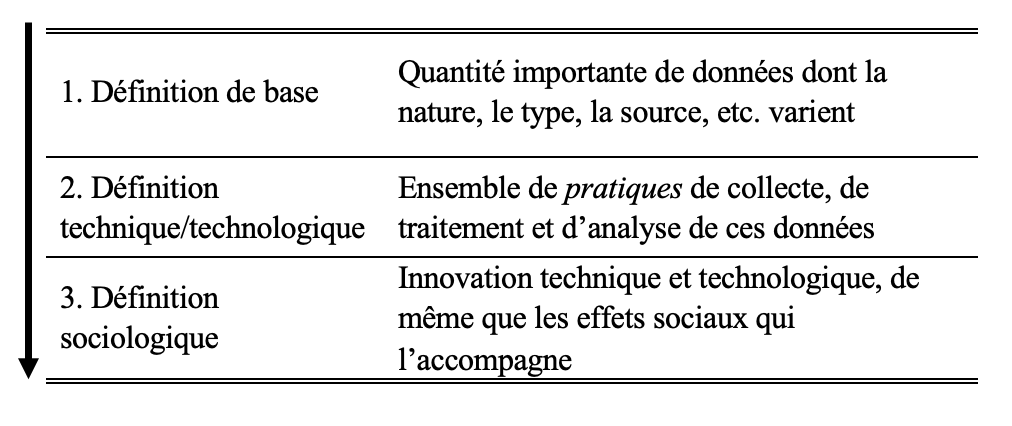
\includegraphics{images/chapitre1_definitions.png} 1. Premièrement, les
données massives représentent une \textbf{\emph{quantité importante de
points d'information}} qui varient selon la nature, le type, la source,
etc. Ici, la distinction entre données massives et données plus
traditionnelles (ou « non-massives ») est simplement quantitative.

\begin{enumerate}
\def\labelenumi{\arabic{enumi}.}
\setcounter{enumi}{1}
\item
  Deuxièmement, les données massives constituent un
  \textbf{\emph{ensemble de pratiques}} de collecte, de traitement et
  d'analyse de ces points d'information. Les données massives
  représentent une technique, c'est-à-dire une manière ou une méthode
  nouvelle de faire de la recherche.
\item
  Finalement, d'une perspective sociologique, les données massives
  représentent les impacts sociaux de ces importants développements
  technologiques. Cette perspective souligne le caractère
  essentiellement social des données massives, en portant notamment
  attention aux risques liés à la confidentialité des données, aux
  enjeux relatifs au consentement et à l'autorisation de collecte des
  informations, aux innovations en intelligence artificielle, etc.
\end{enumerate}

Dans les domaines scientifiques et technologiques, la définition
courante attribuée aux données massives intègre des éléments de ces
trois niveaux d'analyse en se référant à la composition et à la fonction
des données. Premièrement, la \emph{composition} des données massives
est généralement conceptualisée comme comprenant « 4V » : le volume, la
variété, la vélocité et la véracité. Cette conceptualisation jouit d'un
large consensus scientifique (Chen, Mao et Liu, 2014; Gandomi et Haider,
2015; Kitchin et McArdle 2016). Par ailleurs, plusieurs chercheurs ont
élargi cette définition de la composition des données massives en y
incluant, par exemple, la variabilité et la valeur des points de données
(Kitchen et McArdle 2016). Deuxièmement, la \emph{fonction} des données
massives comprend les innovations relatives à l'optimisation, à la prise
de décision et à l'approfondissement des connaissances qui résultent de
leur utilisation. Ces fonctions touchent des domaines sociaux
disparates, incluant le souci d'efficacité et de rendement des secteurs
privé et public ainsi que la recherche scientifique pure (Gartner 2012).

\section*{Les données massives et les sciences
sociales}\label{les-donnuxe9es-massives-et-les-sciences-sociales}
\addcontentsline{toc}{section}{Les données massives et les sciences
sociales}

\markright{Les données massives et les sciences sociales}

Dans le domaine des sciences sociales, les changements causés par
l'utilisation des données massives en recherche sont significatifs.
Plusieurs n'hésitent d'ailleurs pas à les qualifier de changements de
paradigme dans l'étude des phénomènes sociaux (Anderson 2008; Chandler
2015; Grimmer 2015; Kitchin 2014; Monroe et al.~2015). Dans le cas qui
nous intéresse, deux dimensions majeures méritent d'être abordées : (1)
une première relative à la validité (interne et externe) des données
massives et (2) une seconde relative à la différence entre les données
expérimentales et les données observationnelles. Ces deux dimensions
sont présentées de manière simultanées dans les prochaines sections.

\subsection*{La validité de la mesure en sciences
sociales}\label{la-validituxe9-de-la-mesure-en-sciences-sociales}
\addcontentsline{toc}{subsection}{La validité de la mesure en sciences
sociales}

La validité de la mesure constitue une exigence méthodologique centrale
à la recherche en sciences sociales. Les scientifiques cherchent
effectivement à s'assurer que ce qui est mesuré --- par un sondage, une
entrevue, un thermostat ou tout autre outil de mesure --- constitue bel
et bien ce qui est censé être mesuré. Adcock et Collier définissent plus
spécifiquement l'application de la validité de la mesure en sciences
sociales en affirmant que des scores (y compris les résultats de
classification qualitative) doivent capturer de manière significative
les idées contenues dans le concept correspondant (2001: 530).

Toutefois, les problèmes liés à la validité de la mesure sont nombreux
et ont une importance considérable. Dans l'étude des phénomènes sociaux
et humains, la validité de la mesure prend d'ailleurs une complexité
supplémentaire du fait que les données collectées par le biais d'une
mesure constituent le \emph{produit de l'observation} d'un phénomène,
mais non pas le phénomène en soi. Ainsi, lorsque, dans le contexte d'une
recherche, on propose de mesurer l'humeur de l'opinion publique (le
phénomène en soi) sur un enjeu politique, on utilise généralement un
sondage qui a pour fonction de mesurer le pouls d'un échantillon de la
population d'intérêt (ce qui est réellement observé). Cependant, ce que
ce sondage mesure ne constitue pas tout à fait l'opinion publique
elle-même, mais plutôt un segment populationnel qui se veut le plus
souvent représentatif de l'humeur de l'opinion publique. Ceci est tout
aussi vrai pour les sondages à petits échantillons que pour ceux
utilisant des données massives. Autrement dit, la mesure et les données
collectées ne représentent pas le phénomène --- l'opinion publique ---
en soi.

On a déjà mentionné que la validité de la mesure a de l'importance
puisqu'elle garantit que ce qui est mesuré représente réellement ce
qu'on croit mesurer. Toutefois, pour être plus spécifique, dans une
approche positiviste, la validité de la mesure se traduit généralement
par une logique de classification des valeurs attribuées aux différentes
manifestations distinctes d'un même phénomène. Par exemple, une mesure
de la démocratie comme celle proposée par \emph{Freedom House},
fréquemment utilisée en science politique, classifie les libertés
civiles et les droits politiques des États du monde par degré afin de
construire un index, ou une échelle, allant d'un autoritarisme complet à
une démocratie parfaite. Les scores représentent, dans ce contexte, une
mesure artificielle, mais ordonnée et logique, des idées contenues dans
le concept de démocratie telles que libertés civiles et droits
politiques. On peut ainsi dire que la question de la validité de la
mesure est un élément central de ce qui unit (1) le phénomène social
étudié (la démocratie), (2) son opérationnalisation (via les libertés
civiles et droits politiques) et (3) la méthode de mesure utilisée pour
observer et classifier d'une certaine façon le phénomène et les données
qui en découlent (dans le cas de \emph{Freedom House}, des codeurs
travaillant de manière indépendante les uns des autres).

\subsection*{La validité des données
massives}\label{la-validituxe9-des-donnuxe9es-massives}
\addcontentsline{toc}{subsection}{La validité des données massives}

En ce qui a trait aux données massives, la question de la validité de la
mesure constitue un défi nouveau. Les données massives ont en effet
comme avantage d'offrir aux chercheur.e.s soit de nouveaux phénomènes à
étudier, soit de nouvelles manifestations et nouvelles formes à des
phénomènes déjà étudiés. Les données massives permettent donc d'agrandir
la connaissance scientifique.

L'étude de King et al.~(2013) représente un cas éclairant de phénomène
social que l'utilisation des données massives permet désormais
d'étudier. En se basant sur la collecte de plus de 11 millions de
publications en ligne, King et ses collègues ont pu mesurer la censure
exercée par le gouvernement chinois sur ces réseaux sociaux. En
utilisant des données massives nouvelles, les auteurs ont donc pu
observer une manifestation inédite de censure massive qui, sans de
telles données, serait probablement demeurée mal comprise d'une
perspective scientifique. Le nombre de recherches basées sur
l'utilisation des données massives similairement innovantes en sciences
sociales est par ailleurs en croissance constante (Beauchamp 2017; Bond
et al.~2012; Poirier et al.~2020; Bibeau et al.~2021).

Cependant, il faut aussi souligner que les données massives, en raison
de leur complexité, peuvent avoir pour désavantage d'embrouiller l'étude
des phénomènes sociaux. Les opportunités scientifiques liées aux données
massives s'accompagnent en effet de certaines difficultés
méthodologiques. Parmi ces difficultés, trois enjeux sont
particulièrement cruciaux : (1) la validité interne, (2) la validité
externe et (3) la question d'un changement de posture ou d'orientation
épistémologique en sciences sociales causé par les données massives.

\subsubsection*{Validité interne des données
massives}\label{validituxe9-interne-des-donnuxe9es-massives}
\addcontentsline{toc}{subsubsection}{Validité interne des données
massives}

Premièrement, les données massives peuvent représenter un défi à la
validité interne des études en sciences sociales en rendant
pragmatiquement difficile l'établissement de \textbf{\emph{mécanismes
causaux clairs}}. Ce défi est notamment une conséquence du fait que la
plupart des données sont présentement issues d'un processus de
génération (\emph{data-generating process}) qui est hors du contrôle des
chercheur.e.s. Les données massives proviennent en effet habituellement
de sources diverses qui sont externes aux projets de recherche qui les
utilisent. Elles ne sont pas donc générées de manière aléatoire sous le
contrôle des chercheur.e.s.

Un des problèmes liés à cette situation est qu'il est difficile de
garantir une source \emph{exogène} de variation par laquelle les
chercheur.e.s éliminent l'effet potentiel des facteurs confondants
(\emph{confounders}). Règle générale, la distribution aléatoire d'un
traitement et d'un contrôle dans une expérience en laboratoire ou sur le
terrain représente le standard le plus élevé permettant de fournir cette
source exogène de variation, notamment parce qu'elle l'attribution
aléatoire du traitement ou du contrôle est entièrement sous le contrôle
du chercheur.e.s menant l'expérience. Cependant, en ce qui à trait à la
plupart des données massives, elles sont générées de manière
indépendante du contrôle du chercheur.e.s, et sont donc soumises aux
mêmes enjeux et problèmes (biais) que les données observationnelles
traditionnelles.

Pour le dire autrement, le défi de validité interne avec les données
massives constitue un enjeu relatif à la qualité des données. Ce n'est
évidemment pas un défi propre ou unique aux données massives. Ce défi
s'applique également aux autres types de données. Cependant, dans l'état
actuel des choses, le volume et la variété --- deux des 4V --- des
données massives --- textuelles, numériques, vidéos, etc. --- peuvent
miner la qualité de l'inférence causale entre une cause et une
conséquence que permet habituellement un processus contrôlé de
génération des données. En somme, la validité interne des données
massives est une fonction de la qualité de ces mêmes données.

\subsubsection*{Validité externe des données
massives}\label{validituxe9-externe-des-donnuxe9es-massives}
\addcontentsline{toc}{subsubsection}{Validité externe des données
massives}

Deuxièmement, les données massives représentent aussi un défi important
pour la validité externe des recherches en sciences sociales (Tufekci
2014; Lazer et Radford 2017; Nagler et Tucker 2015). Un des problèmes
les plus évidents concerne la \textbf{\emph{représentativité}} des
données massives collectées.

Comme le soulignent Lazer et Radford (2017), la quantité de données, en
soi, ne permet pas de corriger pour la non-représentativité des données.
Les données massives sont ainsi soumises au même problème de biais de
sélection que les autres types de données observationnelles, tels un
sondage ou une série d'entrevues, traditionnellement utilisés en
sciences sociales.

Le cas célèbre de l'erreur de prédiction du \emph{Literary Digest} lors
de la campagne présidentielle américaine de 1936 illustre bien ce
problème. Lors de cette campagne, le \emph{Literary Digest} a prédit à
tort la victoire du candidat républicain Alf Landon sur le président
démocrate sortant Franklin D. Roosevelt, puisque son échantillon de
répondants surreprésentait les électeurs plus aisés, traditionnellement
plus républicains, au détriment des électeurs moins aisés, plus
généralement proches du Parti démocrate. Cette erreur de
surreprésentation dans l'échantillon est due au fait que le
\emph{Literary Digest} a effectué un échantillonnage basé sur les listes
téléphoniques et le registre des propriétaires de voitures, biaisant par
le fait même l'échantillon au détriment des électeurs plus pauvres ne
possédant pas de téléphone ou d'automobile, mais qui constituaient un
électorat favorable à Roosevelt (Squire 1981). Le biais de sélection du
sondage a ainsi sous-estimé le soutien populaire de Roosevelt de plus de
20 points de pourcentage.

Aujourd'hui, l'utilisation des données massives est soumise aux mêmes
enjeux méthodologiques. L'accumulation massive de données ne permet pas
de compenser pour la qualité des données. Les données massives, comme
les données plus traditionnelles, sont soumises aux conséquences
induites par le processus de génération des données (\emph{data
generating process}) comme un échantillonnage.

Toutefois, depuis quelques années, le développement de nouvelles
méthodes de pondération des données offre des pistes de solutions. La
grande quantité de données massives permet notamment d'appliquer des
méthodes de pondération bien plus efficaces pour corriger les
échantillons non-représentatifs (Wang et al.~2015).

\subsection*{Données expérimentales}\label{donnuxe9es-expuxe9rimentales}
\addcontentsline{toc}{subsection}{Données expérimentales}

La question du processus de génération des données devient plus claire
quand on considère comment les \emph{données observationnelles} et les
\emph{données expérimentales} permettent d'effectuer des inférences de
manière distincte (voir Figure 2). Toutefois, pour bien comprendre ce
point, il faut comprendre les notions de données expérimentales et
d'inférence causale, qui sont centrales au domaine de la causalité en
recherche.

En quelques mots, l'essence de la démarche causale se résume comme suit
: le processus de génération de données expérimentales a pour objectif
d'assurer la validité d'une inférence causale estimée sur un échantillon
sur l'ensemble de la population visée.

Plus spécifiquement, le processus de génération des données permet aux
chercheur.e.s de s'assurer que la distribution du traitement entre les
deux groupes, traitement et contrôle, est entièrement aléatoire. De
manière technique, cette distribution aléatoire du traitement entre les
deux groupes permet de garantir une source exogène (à l'opposé de
endogène) de variation sur la variable indépendant (\emph{x). Cette
source exogène de variation permet, quant à elle, d'éliminer
l'endogénéité entre la variable indépendante (}x\emph{) et le résidu
(}e*).

Autrement dit, le fait de distribuer au hasard le traitement entre les
membres du groupe traitement et ceux du groupe contrôle assure que la
variation dans les résultats ne vient pas d'autres facteurs
non-contrôlés (le résidu, \emph{e}), mais plutôt du traitement lui-même
(la variable indépendante, \emph{x}). En distribuant le traitement de
manière aléatoire, on s'assure que les différences dans les résultats
sont vraiment dues au traitement et non à d'autres facteurs.

Il s'agit là d'assurer le respect de la condition d'indépendance,
essentielle à la validité de l'identification de l'effet causal étudié.
Autrement dit, en éliminant l'endogénéité entre la \emph{x} et \emph{e},
on s'assure que l'effet observé n'est pas dû à une variable confondante.

Pour revenir aux données massives, celles-ci ne peuvent pas résoudre les
enjeux liés aux inférences causales ou explicatives (Grimmer, 2015).
Elles sont en effet également soumises aux mêmes impératifs issus du
processus de génération des données.

\subsection*{Données
observationnelles}\label{donnuxe9es-observationnelles}
\addcontentsline{toc}{subsection}{Données observationnelles}

En ce qui a trait aux données observationnelles, il y a deux points
importants. Premièrement, des méthodes d'inférence basées sur des
approches par design (\emph{design-based methods}) comme une méthode de
régression sur discontinuité ou de variable instrumentale peuvent
également garantir des inférences explicatives et causales valides.
Elles nécessitent toutefois plusieurs postulats plus restrictifs dont
l'objectif est d'imiter ou de récréer, de la manière la plus fidèle
possible, une distribution aléatoire du traitement -- ce que la
littérature appelle un \emph{as-if random assignment} (comme si
l'attribution était aléatoire) (Dunning, 2008).

Dans un contexte observationnel, les données massives peuvent donc
permettre d'augmenter la précision des estimations causales.
Effectivement, comme dans un modèle de régression linéaire, plus
l'échantillon est grand, plus l'estimation du coefficient causal ou
probabiliste est précise. Par exemple, un échantillon large dans un
modèle de régression sur discontinuité permet de restreindre la largeur
de bande autour du seuil, garantissant ainsi une distribution presque
parfaitement aléatoire des données et une validité plus élevée à
l'estimation de l'effet causal.

Un autre exemple pourrait être l'utilisation du « matching », souvent
utilisé dans les études économétriques. Supposons que vous souhaitez
estimer l'effet d'un programme éducatif sur les résultats scolaires
d'étudiant.e.s. Le devis de recherche idéal serait d'assigner
aléatoirement les étudiant.e.s au programme (le groupe traitement) ou
non (le groupe contrôle). Toutefois, puisque ce devis idéal peut être
difficilement réalisable, un grand nombre de données pourrait permettre
de trouver pour chaque étudiant.e dans le groupe traitement un
étudiant.e « jumeau » dans le groupe contrôle. Ce « jumeau » serait
similaire en âge, sexe, antécédents socio-économiques, etc. Il serait
ensuite possible de comparer les résultats scolaires de ces jumeaux pour
estimer l'effet du programme. Plus l'échantillon est grand, plus
l'estimation sera précise et fiable, parce qu'il y aura plus de jumeaux
possibles à apparier, réduisant ainsi le biais dû aux variables non
observées.

Il s'agit d'un exemple où les données massives augmentent la validité
interne de l'étude, même si les données sont de nature observationnelle
et non expérimentale.

Deuxièmement, un échantillon de données massives observationnelles
issues d'une plateforme comme X --- anciennement Twitter --- ou Facebook
peut fournir une \emph{description} plus fine de certaines dynamiques
sociales observées sur les réseaux sociaux. Cependant, c'est la manière
dont sont collectées les données de cet échantillon de données massives
qui garantit la représentativité de l'échantillon --- avec pour objectif
l'absence d'un biais de sélection --- et non pas la quantité de données.
Généralement, le biais d'un échantillon est une conséquence de la
non-représentativité des répondants; dans notre exemple, les
utilisateurs des médias sociaux ne sont généralement pas représentatifs
de la population entière.

Dans un tel cas, des méthodes de pondération sur des données
observationnelles peuvent compenser pour la sur- ou la
sous-représentativité de sous-groupes dans un échantillon afin d'assurer
la validité de l'inférence entre échantillon et population. Les données
massives ont ici une importance puisqu'une pondération fiable nécessite
une quantité substantielle d'observations. Une pondération \emph{a
posteriori} sera donc plus fiable plus l'échantillon est grand. Les
données massives ont ainsi une valeur ajoutée afin d'établir des
inférences descriptives plus précises et sophistiquées.

\subsection*{Validité écologique et observation par
sous-groupes}\label{validituxe9-uxe9cologique-et-observation-par-sous-groupes}
\addcontentsline{toc}{subsection}{Validité écologique et observation par
sous-groupes}

Les données massives peuvent aussi jouer d'autres rôles importants
relatifs à la validité externe. Premièrement, les données massives
facilitent effectivement la validité externe de certaines études en
accroissant la validité écologique (\emph{ecological validity}) des
tests expérimentaux, c'est-à-dire le réalisme de la situation
expérimentale (Grimmer, 2015: 81). En effet, la variété des sources et
des formats de données permet aux chercheurs d'imiter plus fidèlement la
réalité sur le terrain vécue par les participants aux études.

Deuxièmement, la quantité importante de données rend possible
l'observation d'effets précis, spécifiques et inédits par sous-groupes
(Grimmer 2015: 81). Alors qu'auparavant, la taille réduite des
échantillons ne permettait pas d'effectuer des inférences valides pour
des sous-groupes de la population --- les écarts-types par sous-groupes
étaient trop grands, rendant difficile l'estimation précise d'un
paramètre comme la moyenne et impossible celle d'un coefficient ---, la
taille énorme des échantillons de données massives permet aux chercheurs
d'estimer des paramètres qui étaient demeurés extrêmement imprécis
jusqu'à aujourd'hui. Notre compréhension des phénomènes sociaux s'en
trouve par le fait même approfondie de façon considérable.

\begin{figure}[H]

{\centering 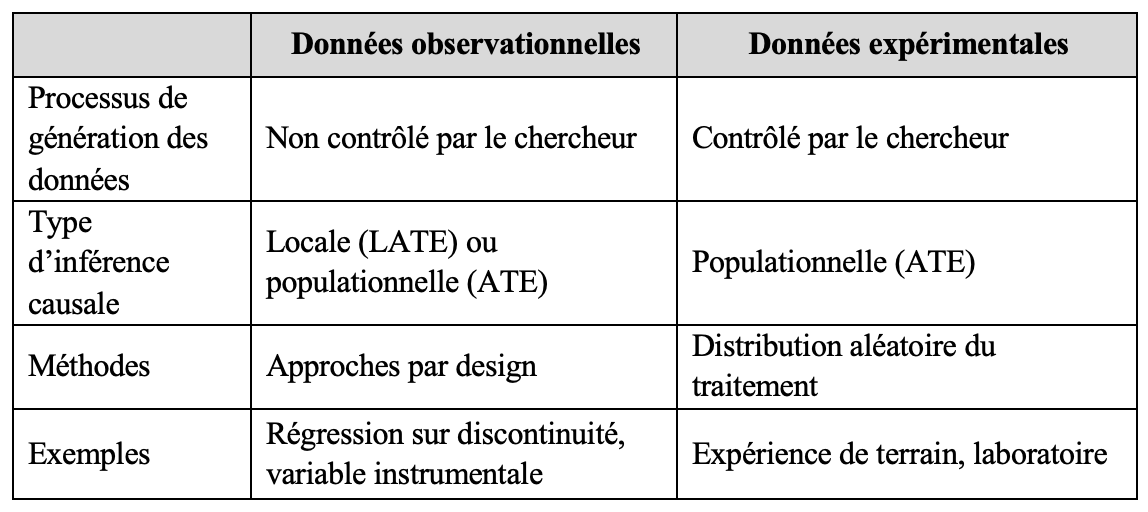
\includegraphics{images/chapitre1_tableau.png}

}

\caption{image2\_2}

\end{figure}%

\section*{Conclusion : trois questions ouvertes pour le
futur}\label{conclusion-trois-questions-ouvertes-pour-le-futur}
\addcontentsline{toc}{section}{Conclusion : trois questions ouvertes
pour le futur}

\markright{Conclusion : trois questions ouvertes pour le futur}

Comme nous venons de le voir, la quantité et la variété nouvelle des
données massives permettent à la fois un approfondissement de l'analyse
de certains phénomènes et l'ouverture de nouvelles avenues de recherche.
L'analyse des données massives peut permettre de mettre en lumière des
tendances subtiles échappant aux ensembles d'informations plus
restreints.

Il faut toutefois souligner que les données massives représentent une
complexification de l'analyse des phénomènes en sciences sociales d'une
perspective non pas seulement méthodologique/technique mais également
épistémologique.

Cela soulève au moins trois questions d'importance, dont les réponses ne
nous sont pas encore accessibles, pour l'avenir de la recherche en
sciences sociales : (1) les données massives entrent-elles
(partiellement du moins) en conflit avec l'impératif de parcimonie qui
caractérise la science moderne?; (2) ces données sont-elles dans la
continuité ou représentent-elles une coupure dans la tradition
béhavioraliste en sciences sociales (et en science politique tout
particulièrement)?; (3) et finalement, de manière reliée, les données
massives proposent-elles ou non une manière de dépasser l'individualisme
méthodologique qui caractérise les sciences sociales contemporaines?

\bookmarksetup{startatroot}

\chapter{Le logiciel libre et le code source ouvert}\label{sec-chap1}

Ce chapitre ne présentera pas un outil en soi. Il vise à initier les
lecteurs à la philosophie du logiciel libre et surtout de situer ces
réflexions dans le contexte de la recherche en sciences sociales. En
fait, l'outil ici est plutôt de l'ordre réflexif que concret. À la fin
de ce chapitre, les lecteurs seront en meilleures positions afin de
situer les outils qui seront présentés dans le grand univers des
logiciels libres et payants. Ils et elles pourront comprendre les
motivations derrière le développement et l'utilisation de tels
logiciels. La création et l'utilisation de logiciels libres dépassent le
simple calcul coûts et bénéfices utilitaires, gratuit contre payant.
Tout cela s'inscrit dans des réflexions philosophiques, éthiques et
épistémologiques plus grandes qui continuent, à ce jour, d'influencer
les développeurs et les utilisateurs. Tout au long de ce chapitre il est
démontré que certaines de ces motivations rejoignent la méthode
scientifique, qui est au coeur de notre quête de savoir et de
compréhension du monde social (\textbf{king\_etal20?}). Ainsi, ce
chapitre jette la base réflexive qui est derrière les choix des outils
numériques présentés dans ce livre, où nous avons tenté de joindre les
avantages des logiciels libres avec certains qui sont payants dans le
but de créer un environnement de travail à la fois individuel et
collaboratif. Avant d'aller plus en profondeur, une certaine distinction
mérite d'être faite, qui permettra de clarifier le but de ce livre et à
la terminologie utilisée.

Il est donc important de faire une première distinction entre une
méthode et un outil numérique. La méthodologie est le champ de la
philosophie des sciences qui s'intéresse à l'étude des méthodes
scientifiques ou techniques. Celles-ci visent à collecter et à analyser
des données, suivant les impératifs scientifiques, et qui ont pour but
de contribuer au savoir et à la connaissance. Il faut faire attention
puisque dans certains ouvrages il est possible que les auteurs décrivent
les méthodes qu'ils ont utilisées comme étant des \emph{outils}. D'un
point de vue méthodologique, lié à la philosophie des sciences, il est
approprié d'utiliser ce genre de vocabulaire. Ainsi, la régression
linéaire, le \emph{clustering}, les entretiens semi-dirigés et l'analyse
de contenu sont des méthodes. En revanche, les outils dits numériques
qui sont présentés dans ce livre ne sont pas des méthodes scientifiques.
Des outils numériques comme \texttt{R}, Dropbox ou GitHub ne sont pas
des méthodes, mais des outils qui permettent de structurer sa pensée,
d'organiser son espace et son environnement de travail, et d'implémenter
son protocole de recherche afin de collecter et d'analyser des données
et d'en dériver des conclusions. Il est donc utile de distinguer les
outils numériques des méthodes.

Ce livre ne vise donc pas à présenter des \emph{outils méthodologiques}
- compris ici comme étant des outils qui permettent de \emph{désigner},
d'exécuter et d'évaluer une recherche (Brady \& Collier, 2010). Le but
est plutôt de présenter des choix \emph{d'outils numériques} qui ont un
fort potentiel d'aider les chercheurs à \emph{structurer leur pensée,
d'organiser leur espace de travail et à implémenter certaines méthodes}.
Cette distinction est importante puisqu'elle définit la distinction
entre ce livre et les nombreux livres de méthodes.

Celles-ci leur permettront de développer un nouveau langage à partir
duquel ils et elles pourront réfléchir et penser leur recherche, et
surtout interagir avec les autres personnes dans leurs champs; avec qui
ils et elles pourront plus aisément collaborer en organisant leur
environnement de travail; avec qui ils et elles pourront partager des
documents et leurs résultats. Ce livre cherche \_\_\_ à guider les
chercheurs dans la \_\_\_ \_\_\_ d'\_\_\_ \_\_\_ dont le nombre ne cesse
de croitre à l'ère numérique. Des choix ont été faits et justifiés sur
la base de différents critères décrits plus loin dans ce chapitre. Après
la lecture de ce livre, le lecteur auront été initié aux langage
distinctif et parfois technique lié aux outils numériques. Surtout, il
sera mieux équipé et informé pour faire ses choix d'outils qui lui
permettront d'être plus efficace en recherche.

Avant toute chose, il est important de commencer pas la base -
comprendre d'où vient le logiciel libre et qu'est-ce que c'est. Le
logiciel libre a, et continu d'avoir, une place importante dans le
développement des outils numériques. Dans les sections suivantes,
l'historique de cette philosophie est présentée afin de mettre en
contraste et mieux comprendre ses motivations et revendications. Après
cette mise en contexte, suit une discussion concrète sur la manière dont
le logiciel payant du logiciel libre sont distingués, avant d'aborder la
différence entre le logiciel libre et le code ouvert. Après coup, nous
aborderons en quoi ces réflexions sont intéressantes et importantes pour
les sciences sociales à l'ère du numérique, ainsi que les avantages et
les inconvénients qui y sont liés. Les outils numériques s'inscrivent
dans chacune des grandes étapes de la recherche - avant, pendant et
après.

Cette discussion sur le logiciel libre se veut une introduction aux
critères qui ont justifiés les choix des outils numériques de ce livre.

\section{Logiciels Libres}\label{logiciels-libres}

\subsection{Le monde du libre}\label{le-monde-du-libre}

\emph{« Vous n'avez pas à suivre une recette avec précision. Vous pouvez
laisser de côté certains ingrédients. Ajouter quelques champignons parce
que vous en raffolez. Mettre moins de sel, car votre médecin vous le
conseille --- peu importe. De surcroît, logiciels et recettes sont
faciles à partager. En donnant une recette à un invité, un cuisinier n'y
perd que du temps et le coût du papier sur lequel il l'inscrit. Partager
un logiciel nécessite encore moins, habituellement quelques clics de
souris et un minimum d'électricité. Dans tous les cas, la personne qui
donne l'information y gagne deux choses : davantage d'amitié et la
possibilité de récupérer en retour d'autres recettes intéressantes. »} -
Richard Stallman (Williams et al., 2010)

Cette analogie illustre bien trois concepts au cœur de la philosophie de
Richard Stallman, souvent considéré comme le père fondateur du logiciel
libre : liberté, égalité, fraternité. Les utilisateurs de ces logiciels
sont libres, égaux, et doivent s'encourager mutuellement à contribuer à
la communauté. Ainsi, un logiciel libre est généralement le fruit d'une
collaboration entre développeurs qui peuvent provenir des quatre coins
du globe. Au centre de ce mouvement se trouve une réflexion éthique à
propos de la liberté des utilisateurs, dont les militants font campagne
depuis le début des années 1980. La Free Software Foundation (FSF),
fondée par Richard Stallman en 1985, définit rapidement le logiciel
«libre» {[}free{]} comme étant garant de quatre libertés fondamentales
de l'utilisateur: 1) la liberté d'utiliser le logiciel sans
restrictions; 2) la liberté de le copier; 3) la liberté de l'étudier; 4)
puis la liberté de le modifier pour l'adapter à ses besoins et le
redistribuer\footnote{La redistribution doit évidemment respecter
  certaines conditions précises, dont l'enfreint peut mener à des
  condamnations
  {[}http://www.softwarefreedom.org/resources/2008/shareware.html{]}}.
Il s'agit ainsi d'un logiciel dont le code source\footnote{Pour rester
  dans les analogies culinaires, le code source est au logiciel ce que
  la recette est à un plat: elle indique les actions à effectuer, une
  par une, pour arriver à un résultat précis. Encore une fois, ce
  dernier peut-être adapté, modifié, bonifié.} est disponible, afin de
permettre aux internautes de l'utiliser tel quel ou de le modifier à
leur guise. L'accès au code source devient essentiel afin de permettre à
l'utilisateur de savoir ce que le programme fait réellement. Seulement
de cette façon, l'utilisateur peut \emph{contrôler} le logiciel, plutôt
que de se faire contrôler par ce dernier (Stallman, 1986).

\subsection{\texorpdfstring{Émergence et sémantique du
\emph{libre}}{Émergence et sémantique du libre}}\label{uxe9mergence-et-suxe9mantique-du-libre}

Plusieurs situent les débuts du mouvement du logiciel libre avec la
création de la licence publique générale GNU, en 1983, à partir de
laquelle va se développer une multitude de logiciels libres. Parmi les
plus populaires, on retrouve notamment le navigateur Firefox, la suite
bureautique OpenOffice et l'emblématique système d'exploitation Linux,
qui se développe d'ailleurs à partir de la licence GNU. Aujourd'hui, il
s'agit d'un véritable phénomène sociétal: des milliers d'entreprises,
d'organisations à but non lucratif, d'institutions ou encore de
particuliers adoptent ces logiciels, dont la culture globale et les
valeurs (entraide, collaboration, partage) s'arriment avec le virage
technologique de plusieurs entreprises. Les logiciels libres ont
différents usages, en passant par la conception Web, la gestion de
contenu, les systèmes d'exploitation, la bureautique, entre autres. Ils
permettent donc de répondre à plusieurs types de besoins numériques et
informatiques.

Il est important de rappeler que le logiciel libre est avant tout une
philosophie, voire un mouvement de société. C'est une façon de concevoir
la communauté du logiciel où le respect de la liberté de l'utilisateur
est un impératif éthique (Williams et al., 2010). Par conséquent, le
terme libre, \emph{free} en anglais, porte à confusion. Celui-ci ne
signifie pas qu'un logiciel libre est nécessairement gratuit. Certes,
plusieurs sont effectivement téléchargeables gratuitement. Toutefois, il
est aussi possible de (re)distribuer des logiciels libres payants. Par
ailleurs, aucun logiciel libre n'est réellement « gratuit » dans la
mesure où son déploiement et son utilisation nécessitent généralement
différents coûts, dont les degrés sont variables en fonction des
compétences et de l'infrastructure dont disposent les utilisateurs (coût
d'apprentissage, coûts d'entretien, etc.). Enfin, il est important de
garder en tête que les logiciels libres possèdent eux aussi une licence
- cette dernière est d'ailleurs garante des libertés que confèrent les
logiciels libres aux utilisateurs.

La grande liberté que ce type de logiciel offre favorise notamment la
collaboration entre les utilisateurs, et ce, à une échelle pouvant être
internationale. Les interactions entre les chercheurs créent une
dynamique d'« innovation ascendante » et d'entraide (Couture, 2014). En
d'autres termes, l'accessibilité et la collaboration favorisent le
développement et l'amélioration de ces logiciels. Selon certains, et
comparativement aux logiciels privés, les logiciels libres ont un niveau
plus élevé d'innovation (Smith, 2002). Contrairement aux logiciels
propriétaires, ceux qui se développent de manière privée et fermée, les
logiciels libres permettent à tous les utilisateurs de participer au
développement. Ceux-ci partagent ensuite leurs améliorations, ce qui
stimule à son tour de nouvelles initiatives. De plus, il est raisonnable
de penser que l'utilité des améliorations, ainsi que l'utilisation qui
en est faite par les utilisateurs, permet de générer un savoir
collaboratif (Couture, 2020).

Il y a aussi certains avantages économiques, dont un faible coût
d'acquisition et de renouvellement pour les particuliers. Cet avantage
individuel génère plusieurs externalités positives. Tout d'abord,
certains logiciels statistiques ainsi que certains programmes
informatiques coûtent plusieurs centaines, voire des milliers de
dollars, et dans certains cas doivent être renouvelés annuellement. Cela
augmente les coûts associés à l'utilisation du logiciel et par
conséquent limite son accessibilité. Comparativement, pour les logiciels
libres, la licence d'acquisition coûte bien souvent moins cher, et aucun
renouvellement de licence n'est demandé dans la plupart des cas.
L'argent sauvé des licences peut alors être investi dans le
développement du logiciel libre (Béraud, 2007). De plus, étant donné que
les chercheurs doivent souvent faire face à des contraintes budgétaires,
les logiciels libres deviennent des outils intéressants afin de
minimiser les coûts de la recherche (Yu \& Muñoz-Justicia, 2022). Il
s'agit d'un avantage encore plus important et intéressant pour les
chercheurs dans les pays du Sud global (Santillán-Anguiano \&
González-Machado, 2023). L'accessibilité de ces ressources permet donc
de réduire l'écart dans la production scientifique entre les pays du Sud
et ceux du Nord. De plus, elle permet à tous de bénéficier d'outils
pédagogiques accessibles, ce qui favorise l'acquisition ainsi que le
développement de compétences méthodologiques.

Dans le cadre d'une formation universitaire, il peut être pertinent
d'enseigner aux étudiants à se servir de logiciels statistiques ou
d'analyse de texte. L'acquisition de ces compétences peut être précieux
tant pour ceux et celles qui souhaitent se diriger vers le milieu
académique, que pour ceux et celles qui visent le marché professionnel.
D'ailleurs sur le site web de la banque d'emplois du gouvernement du
Canada, les conditions d'emplois sont en ce moment\footnote{En date
  d'écrire ces lignes, avril 2024.} très bonnes, et une pénurie de
main-d'œuvre est anticipée, entre 2022-2031, dans les emplois en analyse
de données. Ces compétences sont d'autant plus précieuses aujourd'hui,
dans le monde de données dans lequel nous vivons.

Il est important de souligner que la transition vers les logiciels
libres ne doit pas se faire seulement sur des bases économiques, mais
dans une perspective globale de changement de culture. Changer pour des
raisons purement économiques viendrait à violer l'essence même de la
philosophie du logiciel libre, qui se veut surtout être un esprit de
collaboration et de transparence. Amélioration constante, entraide,
savoir partagé et plusieurs milliers de contributeurs (Couture, 2014),
ces éléments résument très bien la philosophie du logiciel libre.

\subsection{Illustrations}\label{illustrations}

Considérons quelques exemples de logiciels libres et de logiciels
payants afin de mettre en relief les trois éléments présentés ci-haut:
1) la liberté de l'utilisation et de la contribution; 2) les coûts
d'acquisition; et 3) les compétences acquises et développées. Dans les
chapitres suivants, des outils numériques tels que \texttt{R}, SPSS,
STATA, qui permettent de mener des analyses statistiques, ou encore la
suite Office, Quarto, LaTeX, qui permettent de formater un document
écrit, seront présentés. Cette section ne remplace en aucun cas une
lecture approfondie et détaillée des chapitres suivants. Au besoin, nous
recommandons fortement aux lecteurs de se référer au reste du livre. En
ce qui concerne le premier trio, \texttt{R} est le seul logiciel libre
du groupe. Il est accessible gratuitement à partir du site web de CRAN,
et une grande communauté d'utilisateurs contribue activement à son
développement. Par exemple, la compagnie Posit est derrière le
développement de \texttt{RStudio}, Quarto et Positron qui sont toutes
des extensions à code ouvert de \texttt{R}. Ensuite, plusieurs
utilisateurs ont développé des librairies avec des commandes et des
fonctions supplémentaires, qui sont gratuites et dont le code est
disponible sur des plateformes comme GitHub.

Contrairement à \texttt{R}, des logiciels comme SPSS et STATA, qui sont
des logiciels propriétaires, nécessitent une licence privée afin de
pouvoir les utiliser. L'achat d'une licence doit aussi être situé avec
ses propres besoins puisque, dans le cas de SPSS, les licences ne
donnent pas toutes accès aux mêmes fonctionnalités. Ainsi, la licence de
base ne donne pas accès à l'utilisation de la régression, alors que la
licence Premium le permet. De plus, la licence doit être renouvelée tous
les ans, et les prix varient entre 1 700\$ et 5 194\$ pour la licence
web à un seul utilisateur. En ce qui concerne STATA, la logique est
similaire à celle de SPSS. Différents types de licence sont offerts avec
des fonctionnalités supplémentaires, notamment en termes de rapidité de
l'exécution des fonctions et de la capacité à traiter une large quantité
d'observations. Les licences annuelles éducationnelles, donc pour les
étudiants, se situent entre 126\$ et 506\$ par année. Autrement, le prix
varie en 1 248\$ et 1 950\$ par année. De plus, SPSS et STATA sont
développés uniquement par les compagnies IBM et par StataCorp
respectivement. Bien qu'ils n'offrent pas la même flexibilité que
\texttt{R} et que les utilisateurs ne peuvent pas contribuer au
développement au même titre que \texttt{R}, ils offrent d'importantes
ressources pour les utilisateurs, notamment par l'entremise d'un service
à la clientèle, de documentations et de formation web, par exemple.
Ainsi, les utilisateurs sont « pris en charge » directement par la
compagnie afin de leur fournir de l'aide et du support.

En ce qui concerne les langages de balisage, LaTeX ou Quarto peuvent
être utilisés gratuitement sur des interfaces comme \texttt{RStudio} ou
VS Code. Ils offrent donc une grande flexibilité étant compatible avec
plusieurs interfaces. Ainsi, une fois que les compétences avec le
langage ont été développées, il est facile de les transposer d'une
interface à une autre. À l'inverse, la suite Office offre ses propres
interfaces qui sont plutôt intuitives, mais qui contraignent
l'utilisateur à des fonctions prédéfinies. De plus, le coût
d'acquisition d'une licence de la suite Office varie entre 79\$ et 109\$
par année\footnote{Au moment d'écrire ces lignes en 2024}. Similairement
à STATA et SPSS, Microsoft offre plusieurs ressources directement sur
leur site web pour les utilisateurs. Ainsi, un certain ``encadrement''
est offert par la compagnie.

Deux derniers éléments sont importants d'être soulevés. Il ne faut pas
penser que les logiciels libres sont dénués de support et de
documentations. La plupart des logiciels libres, et des extensions comme
les librairies sur \texttt{R}, offrent beaucoup de documentations, et
plusieurs forums d'utilisateurs partagent leurs problèmes et leurs
solutions. De plus, certains tutoriels sont disponibles sur YouTube ou
sur des plateformes comme Datacamp et CodeAcademy. Ainsi, les
utilisateurs ne sont pas totalement laissés à eux-mêmes. De plus,
plusieurs universités offrent des licences pour des logiciels, comme
Office ou SPSS, aux étudiants et aux étudiantes pour éviter que ceux-ci
aient à débourser d'importantes sommes supplémentaires afin d'acquérir
ces logiciels.

\subsection{Logiciel libre et code
ouvert}\label{logiciel-libre-et-code-ouvert}

Parallèlement au logiciel libre, il y a aussi le code ouvert, ou
\emph{open source}. A priori, la dénomination du logiciel libre et celle
du \emph{code ouvert} semblent suggérer qu'il s'agit de synonymes. Dans
les deux cas, le lecteur pourrait croire que l'on fait référence à des
logiciels, par exemple, qui sont exempts de restrictions d'utilisations
et auxquelles les utilisateurs peuvent participer au développement.
Cependant, il y a une distinction importante entre les deux.

Bien que les deux renvoient sensiblement aux mêmes types de logiciels,
les tenants de ces approches ne partagent pas la même perspective. Comme
Stallman (2022) l'explique, le logiciel libre est d'abord et avant tout
un mouvement qui fait « campagne pour la liberté des utilisateurs de
l'informatique ». Le code ouvert, quant à lui, met l'accent sur les
avantages pratiques, plutôt que de militer pour des principes.

Le terme \emph{code ouvert} sera introduit seulement en 1998 afin de
clarifier l'ambiguïté dans la dénomination « logiciel libre »
\footnote{Soit ceux qui ont été conçus suivant les principes
  philosophiques et éthiques qui sous-tendent ce mouvement.}, \emph{free
software} en anglais, afin de spécifier que le code source était
accessible, et non pas que le logiciel était « gratuit » (Ballhausen,
2019). De plus, les logiciels à code ouvert doivent respecter un certain
nombre de critères quant à la distribution de leurs logiciels (Open
Source Initiative, 2006).

Rappelons tout d'abord que le logiciel libre se définit sur la base de
quatre libertés: 1) liberté d'utiliser le programme comme désiré; 2)
liberté d'étudier le fonctionnement du programme et de le modifier pour
ses propres besoins; 3) liberté de redistribuer des copies; 4) liberté
de distribuer des copies de la version « améliorer » du programme pour
ses pairs (Ballhausen, 2019). Concernant le \emph{code ouvert}, tout
logiciel qui souhaite être inclus sous cette appellation doit respecter
dix critères: 1) Redistribution gratuite; 2) doit inclure le code
source; 3) doit permettre les modifications et les travaux dérivés; 4)
l'intégrité du code source; 5) ne doit pas discriminer des personnes
et/ou groupes; 6) ne doit pas restreindre personne dans l'utilisation du
logiciel pour un domaine d'activité; 7) distribution d'une licence pour
l'utilisation; 8) la licence ne doit pas être spécifique pour un
produit; 9) la licence ne doit pas placer de restriction sur d'autres
programmes; 10) la licence doit être technologiquement neutre\footnote{Pour
  plus d'informations sur ces caractéristiques, nous encourageons les
  lecteurs à se référer au lien web de Open Source Initiative (2006).
  Ils y trouveront un contenu détaillé pour chacune des caractéristiques
  susmentionnées.} (Open Source Initiative, 2006).

Il est aussi utile de les distinguer des logiciels « non libres », soit
les logiciels propriétaires: « Son utilisation, sa redistribution ou sa
modification sont interdites, ou exigent une autorisation spécifique, ou
sont tellement restreintes qu'en pratique vous ne pouvez pas le faire
librement » (Système d'exploitation GNU, 2023). Par contraste, la
licence libre confère des droits de propriétaire. L'utilisateur a le
droit d'installer le logiciel sur autant d'ordinateurs que désiré, le
modifier selon ses besoins et le distribuer avec ou sans ses
modifications. Il peut même demander d'être payé pour distribuer des
copies, avec ou sans ses modifications.

Le logiciel libre et le \emph{code ouvert} ont certaines similitudes
puisqu'ils adhèrent tous les deux à la même vision du logiciel, ainsi
que de son accessibilité. Toutefois, il est important tout de même de
les distinguer puisqu'ils ont des origines différentes, et qu'ils mènent
à certaines pratiques qui sont différentes. La prochaine section utilise
un cas concret afin d'expliquer l'effet du libre, et l'utilité que cela
peut avoir.

\section{Les sciences sociales à l'ère du numérique: les enseignements
de la philosophie du logiciel
libre}\label{les-sciences-sociales-uxe0-luxe8re-du-numuxe9rique-les-enseignements-de-la-philosophie-du-logiciel-libre}

En quoi est-ce que ces deux concepts, issus du monde de l'informatique,
sont-ils intéressants et/ou importants pour les sciences sociales ? Pour
répondre à cette question, il est important de retourner à la base, soit
de se questionner sur ce que constitue la recherche scientifique dans
les sciences sociales.

Dans leur célèbre ouvrage \emph{Designing Social Inquiry}, King et al.
(2021)\footnote{Ce livre est aussi connu sous l'acronyme \emph{KKV}, en
  référence à la première lettre du nom de famille de chacun des
  auteurs.} propose quatre critères qui définissent la recherche dite
scientifique: 1) le but est l'inférence; 2) les procédures sont
publiques; 3) les conclusions sont incertaines; 4) le contenu est la
méthode. La philosophie du code ouvert et les avantages pratiques du
logiciel libre s'arriment parfaitement avec plusieurs de ces critères.

Plusieurs outils numériques rendent possibles le partage et l'accès
public des données et de la méthode utilisée; rejoingnant ainsi le
critère de la transparence des procédures et celui de la méthode comme
étant le contenu. Certains de ces outils seront d'ailleurs abordés dans
les chapitres suivants. L'accès aux données et aux procédures d'analyse
est un impératif scientifique. Comme nous l'aborderons un peu plus loin,
il y a toujours des concessions à faire lors des investigations
scientifiques. Par conséquent, un meilleur accès aux procédures et aux
données utilisées permet de cibler plus facilement les limites de
certaines recherches et de les combler lors de recherche ultérieure. De
plus, l'arrivée des données massives ouvre de nouvelles portes, mais
surtout de nouveaux défis relatifs à la validité interne et externe
ainsi qu'au type de données récoltées et à la validité écologique. Le
livre de Marres (2017) est très intéressant à ce sujet. Face au constat
que la vie sociale se trouve affecter par les changements numériques, il
nous faut en tant que chercheur du monde social réfléchir à notre façon
de comprendre les changements qui s'opèrent. Ainsi, face à ces défis,
une des solutions se trouve notamment dans un meilleur partage et dans
une meilleure accessibilité aux données et aux procédures.

Il est possible de faire certains liens avec les deux autres critères de
King et al. (2021). Premièrement, comme le but de la science est
l'inférence, soit tenter d'expliquer des phénomènes sociaux qui
s'inscrivent dans des catégories plus larges que nos observations
directes\footnote{Par exemple, les mouvements sociaux, le comportement
  électoral, les guerres et les révolutions, et bien plus.}, il est
important que nos conclusions soient soumises au plus grand nombre
possible et pas uniquement au comité éditorial d'une revue scientifique.
D'une part, la validité de nos résultats a un potentiel politique
important. Plusieurs décisions peuvent être prises sur la base des
connaissances et de la compréhension des dynamiques sociales. Il est
donc important que les résultats de recherche qui informent ces
décisions soient le plus rigoureux possible, et qu'ils aient été soumis
à l'examen critique par le plus grand nombre d'individus. D'autre part,
et comme King et al. (2021) le font remarquer, les conclusions sont
toujours incertaines. L'examen critique et la reproduction des
protocoles sont donc une nécessité dans ce contexte d'incertitude
constant. La science ne cherche pas à être dogmatique. Au contraire,
l'incertitude caractérise bien la science. Les résultats sont toujours
incertains, et ce que la recherche vise à faire c'est de renforcer notre
niveau de confiance envers certaines explications tout en écartant les
explications alternatives. Comme plusieurs de ces phénomènes ne sont pas
homogènes et qu'ils ne sont pas immuables, les explications ainsi que
notre compréhension de ces dynamiques doivent être constamment revus.

Dans la même lancée, l'ouvrage \emph{Rethinking Social Inquiry} (Brady
\& Collier, 2010), une réponse à King et al. (2021), partage, en partie,
cette définition de la recherche scientifique. Pour les auteurs, les
scientifiques du monde social possèdent plusieurs outils qui leur
permettent de \emph{designer}, \emph{d'exécuter} et \emph{d'évaluer} une
recherche. Ces outils sont des procédures et des pratiques employées par
les chercheurs des traditions quantitatives et qualitatives. Ils ont
aussi des techniques analytiques qui leur permettent de \emph{développer
des preuves qui sont convaincantes}\footnote{L'objectif des auteurs est
  de permettre le dialogue et la réconciliation entre les tenants des
  deux principales traditions méthodologiques: les quantitativistes et
  les qualitativistes. D'où leur vision de la science comme se devant de
  développer des preuves qui seront considérées comme convaincantes par
  les chercheurs de ces deux traditions.}.

Chacun de ces outils a toutefois ses forces et ses faiblesses. Inspiré
de Przeworski \& Teune (1970), Brady \& Collier (2010) parlent ainsi de
\emph{compromis}. Selon eux, la pertinence d'un outil méthodologique
dépend de la question de recherche, du but de la recherche et de son
contexte. Le choix d'un outil, sur cette base, entraîne des compromis
qui empêchent d'atteindre tous les buts analytiques simultanément. Même
lorsqu'il y a adéquation entre la question et la méthode, plusieurs
autres embuches peuvent entraîner ces compromis, comme la disponibilité
des données par exemple, qui limitent par la suite la qualité et la
précision des résultats, ce qui explique, en partie, l'incertitude
envers les conclusions.

En sommes, les enseignements de la philosophie du code ouvert, les
avantages pratiques du logiciel libre et les outils qui en découlent ont
le potentiel de permettre non seulement une plus grande transparence des
protocoles scientifiques, mais aussi un plus grand partage du savoir, et
ce, du début de la recherche jusqu'à la publication des résultats.

\section{Inconvénients et défis}\label{inconvuxe9nients-et-duxe9fis}

Jusqu'à présent, il a surtout été question des avantages liés aux
logiciels libres. Toutefois, il n'y a pas que des points positifs, et ne
pas aborder certaines limites serait malhonnête.

\subsection{La courbe d'apprentissage}\label{la-courbe-dapprentissage}

Dans leur texte, Paura \& Arhipova (2012) soulèvent une critique faite
envers certains logiciels libres, notamment envers \texttt{R}. Le
problème principal d'enseigner avec des logiciels libres est qu'ils
peuvent être compliqués à apprendre ainsi qu'à utiliser; par conséquent,
les étudiants passeraient plus de temps à tenter de résoudre les erreurs
de programmation plutôt que d'apprendre et de mener leurs
analyses\footnote{Sur cet enjeu, nous conseillons aux lecteurs et
  lectrices de lire le chapitre 2 sur les langages de programmation
  ainsi que le chapitre 8 sur l'intelligence artificielle. Plusieurs
  trucs et astuces seront présentés dans ces chapitres.}. Par exemple,
\texttt{R} demande l'apprentissage d'un langage de programmation afin de
pouvoir utiliser le logiciel à son plein potentiel. De plus, la syntaxe
de certaines librairies demande aussi un certain temps d'adaptation. À
titre de comparaison, le logiciel SPSS offre une interface beaucoup plus
intuitive que \texttt{R}, dans lequel l'utilisateur peut simplement
cliquer sur les différents menus dans la barre d'outils afin de
sélectionner les analyses qu'il ou elle souhaite faire. SPSS présente
ses résultats dans des tableaux qui sont clairs et lisibles,
contrairement à \texttt{R} où plusieurs fonctions présentent les
résultats directement dans la console, sous un format moins
``esthétique''. De plus, la plupart des logiciels payants viennent avec
un certain service à la clientèle. En d'autres termes, lorsque les
utilisateurs rencontrent des problèmes techniques, ils peuvent se
référer au manuel d'utilisateur ou bien par l'entremise de l'assistance
technique qui est offerte par la compagnie. À l'opposé, la plupart des
logiciels libres ne sont pas accompagnés d'un service à la clientèle.
Les utilisateurs doivent donc se « débrouiller » par eux-mêmes
lorsqu'ils rencontrent des difficultés et des problèmes.

Toutefois, lorsque l'on compare le coût d'apprentissage avec les
bénéfices tirés, il est plus difficile de soutenir qu'il s'agit
uniquement d'un désavantage. Dans un premier temps, la syntaxe de
programmation de \texttt{R} n'est pas parmi les plus complexes à
apprendre, et elle s'intègre très bien avec certaines extensions, dont
Quarto ou RMarkdown, qui offrent de multiples possibilités pour
transmettre le résultat de ses recherches, que ce soit par l'entremise
d'un rapport, d'un article scientifique, un site web ou même un blogue.
Surtout, la logique derrière la syntaxe de base de \texttt{R} et celle
d'une nouvelle librairie reste sensiblement inchangée. Par conséquent,
lorsque nous avons une bonne compréhension du fonctionnement de base de
\texttt{R}, l'apprentissage d'une nouvelle librairie se fait
relativement rapidement. Certaine, comme \texttt{dplyr} du
\texttt{tidyverse} facilite grandement la manipulation des données
comparativement aux commandes de base. Dans un deuxième temps, en
comparant le coût, soit d'apprendre le langage de \texttt{R}, avec les
bénéfices, de mener ses propres analyses de données et de formater les
résultats pour les présenter, il est assez clair que tous ceux et celles
qui souhaitent, de près ou de loin, travailler avec des données
quantitatives, les bénéfices dépassent largement le coût. D'autant plus
que ces compétences s'inscrivent dans la longue durée, alors que
l'apprentissage est plutôt de courte à moyenne durée. Dans un troisième
temps, bien que certains logiciels offrent des CMDernatives plus
intuitives, elles n'offrent pas la même flexibilité que la plupart des
logiciels libres offrent. Pour résumer, bien que l'apprentissage d'un
langage de programmation demande un investissement en temps, les
bénéfices générés par ces nouvelles compétences dépassent le coût
initial. Finalement, bien que les logiciels libres n'offrent pas de
service à la clientèle, il existe bien souvent des forums d'utilisateurs
sur le web, tel que \emph{Stackoverflow} où il est possible de trouver
des réponses à ses questions et/ou de poser ses questions. Par
conséquent, bien qu'il ne s'agit pas d'un service directement offert par
l'outil numérique en question, il est toujours possible de trouver du
support et de l'aide par l'entremise de la communauté d'utilisateur.

\subsection{Problème de transparence}\label{probluxe8me-de-transparence}

L'arrivée des sciences informatiques a fait émerger des problèmes de
reproductibilité des protocoles scientifiques (Janssen, 2017). Le
problème principal est relatif à l'accès au code utilisé par les
chercheurs. Par exemple, il est possible de réaliser des analyses
statistiques avec \texttt{R} sans partager le code utilisé, ce qui
limite la transparence du processus scientifique. Dans cette situation,
il est difficile de savoir si des erreurs de codage ont été commises,
volontairement ou involontairement, affectant ainsi les résultats
partagés.

Afin de remédier à ce problème, certains outils tels que
GitHub\footnote{une plateforme publique \emph{code ouvert} sur laquelle
  nous pouvons héberger et partager notre code.} participent à la
transparence des résultats scientifiques (Fortunato \& Galassi, 2021).
Ce logiciel permet aux chercheurs de partager leur code afin qu'il
puisse être accessible pour tous. Il est important de mentionner ici que
l'installation et la configuration de GitHub peuvent s'avérer difficiles
pour ceux et celles qui ne sont pas initiés à l'informatique. Cela
constitue une certaine barrière dans son utilisation. Toutefois, nous
souhaitons tout de même présenter l'utilité de ce logiciel puisqu'il
permet de rendre les processus ainsi que les résultats de recherche plus
transparents. Par exemple, si l'on réalise une analyse statistique de la
relation entre l'économie et le vote, nous pourrions partager l'ensemble
du code que nous avons utilisé sur GitHub. D'une part cela permettrait
aux utilisateurs de vérifier si les résultats sont honnêtes, et d'autre
part de réutiliser le code pour mener leurs propres analyses.

Cependant, le partage du code reste encore majoritairement volontaire.
Janssen et al. (2020) soutiennent que plus d'effort et d'actions
concertés doivent être mis en place afin d'améliorer l'accessibilité aux
codes. Toujours selon ces auteurs, les journaux scientifiques pourraient
exiger que les auteurs rendent leur code public lors du processus de
publication. D'ailleurs, les résultats d'une expérience sur les facteurs
qui influencent les chercheurs à partager leur code démontrent que les
initiatives individuelles ne seront pas suffisantes pour une
augmentation du partage du code (Krähmer et al., 2023). Par conséquent,
rendre le code accessible devrait devenir un standard institutionnalisé.

\subsection{Appropration commerciale}\label{appropration-commerciale}

Dans ce cas-ci, il s'agit plutôt d'un défi auquel le logiciel libre est
confronté plutôt qu'une critique quant aux limites de son utilisation.
En fait, l'accès au code source ainsi que la liberté et la possibilité
de contribuer au développement du logiciel constitue un avantage
intéressant pour les compagnies privées. Par conséquent, nous avons
assisté à une intégration partielle du logiciel libre dans la logique
capitaliste (Bessen, 2002; Broca, 2013). Certaines compagnies
profiteraient des utilisateurs comme une main-d'œuvre gratuite afin de
bonifier leur logiciel, ce qui permet, dans certains cas, de générer des
revenus commerciaux dont l'entreprise est la seule bénéficiaire
(Couture, 2020). Attention, il ne faut pas penser que toutes les
compagnies agissent de manière prédatrice. Le but ici est de souligner
que certaines pratiques commerciales trouble l'essence du mouvement du
logiciel libre, qui se veut davantage être un outil de collaboration
accessible, plutôt qu'un moyen pour générer des profits. Il est
important de garder en tête les valeurs et la philosophie qui a donné
lieu à ce mouvement.

\section{La chronologie de la
recherche}\label{la-chronologie-de-la-recherche}

Malgré ces limites et ces défis, nous pensons que les différents outils
numériques ont leur place en sciences sociales, et qu'ils s'inscrivent
parfaitement à chaque étape de la recherche. Bien que le partage soit
encore majoritairement sur une base volontaire, adopter cette pratique
dès maintenant est important pour s'engager vers une science plus
ouverte et transparente. Quant à cette dernière caractéristique, il ne
faut pas croire que le partage des résultats se limite à une conférence
ou à une publication scientifique. Bien au contraire, tout chercheur qui
souhaite être le plus transparent doit s'engager dans ce processus dès
la conception de sa recherche.

Avant de présenter différents outils qui existent pour cela, il faut
préciser en quoi la transparence et l'accessibilité sont bénéfiques pour
tous. D'une part, et comme nous l'avons présentée dans la section
précédente, la transparence est une caractéristique fondamentale de
toute recherche qui se veut scientifique. Elle est aussi liée à
l'intégrité du chercheur. Il est impératif de faire état du processus
qui mène à notre conclusion, de la sélection de nos données jusqu'à
l'analyse. C'est de cette façon que nous pouvons juger de la validité et
de la fiabilité des inférences, et surtout de ses limites. D'autre part,
la transparence favorise aussi l'apprentissage (King et al., 2021). De
rendre publique et accessible, à l'aide des outils numériques, les
données, le code et la ou les méthodes utilisées permet de contribuer
non seulement aux débats méthodologiques, mais aussi permet à d'autres
chercheurs d'apprendre sur l'utilité et l'utilisation de ces méthodes.

\subsection{Avant la recherche}\label{avant-la-recherche}

Au fil des prochains chapitres, les lecteurs apprendront un nouveau
jargon. Au même titre qu'une langue comme le français, l'anglais ou le
japonais, ce langage permet de communiquer, et surtout de réfléchir. De
nouveaux concepts, une façon de penser et de réfléchir à leur recherche,
et surtout à son organisation. C'est au travers de la langue que nous
pouvons réfléchir. Ainsi, à l'aide de ces termes, les lecteurs seront
outillés pour concevoir leur recherche et leur organisation avant même
de l'entamer. De la visualiser dans toute son ampleur, de cibler leurs
besoins en fonction de leur but et de leurs intérêts et ainsi organiser
leur environnement de travail en conséquence.

De plus, motivée par cet objectif inhérent à la science, la transparence
exige du chercheur un engagement dès les premières étapes de sa
recherche. Tout d'abord, il peut déjà établir son \emph{workflow} en
créant son dépôt GitHub dans lequel il rendra accessibles son code et
ses données. Plus d'informations sont présentées dans le chapitre 3.
Ensuite, une fois le \emph{design} de recherche\footnote{Généralement,
  un design de recherche comprend les éléments suivants: Introduction,
  revue des écrits, problématiques, une question de recherche, un cadre
  théorique, des hypothèses ainsi qu'une section sur la méthode et les
  données utilisées.} fait, le ou la chercheur peut le préenregistrer
sur le site web de \emph{Open Science Framework}\footnote{Lien vers le
  site web: https://osf.io}. L'objectif de ce site web est que les
chercheurs puissent faire état de leurs hypothèses avant la collecte et
l'analyse des données afin d'éviter toute manipulation malhonnête
\emph{post hoc}. Il s'agit d'un mécanisme qui se veut contraignant afin
que les chercheurs s'en tiennent à ce qu'ils ou elles avaient prévu de
mener comme recherche.

\subsection{Pendant la recherche}\label{pendant-la-recherche}

Une fois la recherche débutée, plusieurs outils s'offrent pour une
gestion efficace du flux de travail. Plusieurs d'entre eux sont
présentés dans les chapitres suivants. Ces outils permettent notamment
de sauvegarder les données et l'avancement du projet sur des serveurs
externes (le \emph{cloud}), comme Dropbox, afin d'éviter de tout perdre
en cas de problème. D'autres permettent de produire le matériel
nécessaire pour l'analyse de nos données, tel que R. Certains permet
aussi de partager avec des collaborateurs l'avancement de notre projet
et les scripts de nos analyses, comme Git et GitHub. D'autres permettent
de structurer notre texte pour la production d'un article scientifique
ou d'un chapitre de livre, comme Overleaf et Quarto. Ils permettent
notamment d'ajouter des tableaux et des graphiques tirés directement des
analyses, le tout dans un format respectant les exigences matérielles
pour la publication.

Il y a également des limites à tous ces outils. Chaque chapitre de ce
livre présentera les points positifs et négatifs des outils qui y sont
abordés.

\subsection{Après la recherche}\label{apruxe8s-la-recherche}

Une fois l'article écrit et publié, les auteurs peuvent décider de
rendre accessible le matériel produit et utilisé en version gratuite sur
le web. Il s'agit du \emph{open science}, ou de la \emph{science
ouverte} (Chakravorty et al., 2022).

Cela permet de rendre non seulement les publications accessibles à tous
sur internet gratuitement, mais aussi les données utilisées, par
exemple, pour la réalisation de l'étude. Ces données peuvent ensuite
être réutilisées par d'autres chercheurs. Il s'agit d'avantages très
importants, et surtout très prometteurs. D'une part, un plus grand accès
au savoir scientifique aux décideurs publics permettra de prendre des
décisions qui s'appuient sur la science, et idéalement, sur une
pluralité de sources scientifiques afin de pouvoir évaluer adéquatement
les effets positifs et négatifs. Finalement, la réutilisation des
données peut réduire considérablement les coûts de la recherche. Bien
souvent, la production des données peut engendrer des coûts importants.
Par exemple, la production d'un sondage peut coûter plusieurs milliers
de dollars, et les données sont bien souvent utilisées qu'une seule fois
. Le partage des données de manière gratuite permet à des chercheurs qui
n'ont pas toujours les moyens de financer un sondage d'avoir accès à des
données. En somme, il s'agit de décloisonner le savoir des milieux
académiques. Ce qui vaut non seulement pour les publications, mais aussi
pour les données et les protocoles de recherche.

Toutefois, le libre accès reste confronté à certains défis. D'une part,
il y a un transfert de la charge financière qui se fait parfois vers les
chercheurs et les universités. Afin que les publications soient
accessibles en libre accès, les chercheurs et les universités doivent
souvent payer des sommes importantes. Cela soulève plusieurs questions
quant aux capacités des universités du Sud global et pour les chercheurs
hors universités, par exemple, de pouvoir assumer la charge financière
qui est liée à la publication en accès libre (Greussing et al., 2020).
D'autre part, bien que plusieurs pensent que les données ouvertes et la
science ouverte puissent contribuer à réduire les inégalités dans la
production du savoir entre le Nord et le Sud, certains restent
sceptiques quant à ce scénari(\textbf{powell\_etal20?}). En fait, les
données ouvertes permettent de réduire les coûts d'accès aux données,
mais ne réduisent pas les coûts de production pour autant. Par
conséquent, un scénario évoqué par Serwadda et al. (2018) est un retour
à la recherche parachute\footnote{La recherche parachute est une «
  pratique extractive par laquelle des chercheurs - généralement issus
  de pays dotés de ressources élevées - effectuent des recherches et
  extraient des données et des échantillons de régions ou de populations
  autochtones, généralement des contextes ou des pays à faibles
  ressources, sans reconnaître de manière appropriée l'importance de
  l'infrastructure et de l'expertise locales. Ce faisant, les chercheurs
  étrangers ne parviennent pas à établir des collaborations équitables
  et à long terme avec des partenaires locaux. » (Odeny \& Bosurgi,
  2022)}. En d'autres termes, les chercheurs du Sud resteraient des
acteurs de second plan, et qui pour étudier leur propre société,
devraient utiliser des données de chercheurs du Nord qui auraient été
produits sans la participation des chercheurs locaux. Finalement, il y a
aussi des enjeux quant à la confidentialité des répondants et des
utilisateurs (Chiware \& Skelly, 2023). Plusieurs individus, comme dans
le cas d'entretiens ou d'un sondage, vont accepter de participer à
l'enquête parce que leurs réponses seront anonymisées et qu'elles ne
seront pas partagées publiquement. Tous ces éléments soulèvent
d'importantes réflexions éthiques quant aux bonnes pratiques à
développer dans le cadre de la science ouverte. La science ouverte à un
avenir très prometteur et peut générer des retombées positives, à
conditions quelle s'intéresse aux différents défis auxquels elle est
confrontée.

\section{Critères de sélection}\label{crituxe8res-de-suxe9lection}

Étant donné que le but de l'ouvrage n'est pas uniquement d'offrir une
perspective sur le monde du numérique, mais surtout d'offrir des
conseils pratiques aux lecteurs, certains choix ont dû être faits dans
la sélection des outils. Bien que ces choix soient arbitraires, ils sont
tout de même informés par certains critères. Au moment d'écrire ces
lignes, peu de littérature existe sur le sujet. Par conséquent,
l'élaboration de ces critères s'est faite de manière inductive, soit à
partir de l'expérience des auteurs. Ces critières sont aussi informés
par des considérations pratiques, tels que la popularité de
l'utilisation par une communauté et par un champ d'études des sciences
sociales.

Six critères jugés pragmatiquement bénéfiques pour la recherche
constituent la d'évaluation de chacun des outils. Ainsi, bien que le
logiciel libre ait été mis de l'avant tout au long de ce chapitre, ce ne
sont pas tous les outils numériques présentés dans ce livre qui sont
issus du monde du logiciel libre. En fondant nos évaluations et nos
choix sur des considérations pratiques, certains logiciels payants sont
parfois recommandés même lorsqu'une version libre existe. Par exemple,
l'utilisation coûte que coûte, voire idéologique, de certains outils
issus du monde du logiciel libre peut cloisonner les chercheurs entre
les utilisateurs et les non-utilisateurs de ces logiciels. D'où
l'importance de conidérer d'autres critères afin de s'assurer que ce
soit la collaboration scientifique qui soit optimisée, et non un
principe idéologique ou philosophique.

Les lecteurs sont encouragés à réfléchir à propos de leur propre besoin
afin de déterminer quels outils qui répondent le mieux à leurs besoins
individuels et collectifs. Par exemple, si dans leur communauté, les
gens utilisent Python plutôt que R, alors nous recommandons d'utiliser
Python. En d'autres termes, les critères et les outils de ce livre ne
visent pas un dogmatisme, et un rejet total de tous les autres outils
qui ne sont pas couverts dans ce livre. Il est important d'évaluer ses
besoins afin de choisir quels outils devraient être utilisés.

\subsection{Accessibilité (Gratuit ou peu
dispendieux)}\label{accessibilituxe9-gratuit-ou-peu-dispendieux}

L'accessibilité au plus grand nombre de ces outils est importante pour
l'atteinte d'une science plus inclusive, et qui respecte les moyens de
chacun. L'accès à des outils de qualité ne devrait pas être caché par
des verrous d'accès payants.

Cette accessibilité est aussi importante pour deux autres raisons. La
première, comme le livre vise à donner des connaissances pratiques dans
l'utilisation de ces outils numériques, il est important que les
lecteurs aient facilement accès à ce qui sera présenté. Cela permettra
de reproduire au fur et à mesure de la lecture les différentes étapes et
pratiques qui sont présentées. La deuxième, est un corolaire du premier,
une fois ces compétences acquises, les lecteurs pourront facilement les
réutiliser pour réaliser les diverses tâches qu'ils et elles ont besoin
d'accomplir.

\subsection{Existence d'une communauté
d'utilisateurs}\label{existence-dune-communautuxe9-dutilisateurs}

Ensuite, l'existence d'une communauté d'utilisateur pour les différents
outils qui sont présentés dans ce livre a été considéré comme important.
Ces communautés permettent une grande collaboration entre les différents
utilisateurs, et servent souvent de forum d'aide lorsque des problèmes
surviennent. Par conséquent, les lecteurs auront accès à plusieurs
forums d'aide sur internet, au besoin, pour la plupart des outils qui
sont présentés dans ce livre. Ainsi, au besoin, ils auront accès à des
ressources supplémentaires en ligne lorsqu'une question ou un problème
surviendra.

Il se peut que certains logiciels libres n'aient pas un guide
d'utilisateur qui soit fourni avec le téléchargement du logiciel.
Parfois, cela peut être difficile pour ceux qui souhaitent apprendre à
utiliser certains de ces outils de se retrouver et de répondre aux
questions qui surviennent. C'est pour ces raisons que nous avons
considéré l'existence d'une communauté d'utilisateurs, et l'existence de
forum d'aide sur le web. Par exemple, pour toutes les questions liées au
code, nous pouvons aller sur le site web de \emph{Stack Overflow}, qui
est un important forum d'échange, et sur lequel nous pourrons trouver
plusieurs informations et réponses à nos questions.

\subsection{Popularité en sciences
sociales}\label{popularituxe9-en-sciences-sociales}

Nous avons choisi certains outils sur d'autres notamment à cause de leur
popularité dans les disciplines en sciences sociales. Par exemple, en
sciences sociales, pour les analyses quantitatives, c'est le logiciel R
qui est prédominant aujourd'hui. Non seulement dans son utilisation,
mais aussi dans des formations méthodologique au prestige international,
comme dans le cadre de la \emph{Inter-university Consortium for
Political and Social Research} (ICPSR), \emph{Essex Summer School in
Social Science Data Analysis}, \emph{The European Consortium for
Political Research}, et bien d'autres. Par conséquent, il s'agit d'une
considération pratique. Dans le monde du numérique et de la
programmation, certains de ces outils deviennent une forme de langage.
Ainsi, la maîtrise de ce langage permet de dialoguer avec les autres
chercheurs de notre champ, ce qui favorise les débats et la recherche
collaborative, par exemple.

\subsection{Compatibilité avec d'autres
outils}\label{compatibilituxe9-avec-dautres-outils}

Plusieurs des outils que nous présentons sont issus de notre expérience
de recherche. Nous utilisons plusieurs d'entre eux notamment parce
qu'ils permettent une certaine synergie dans le processus de la
recherche. Ainsi, ils s'intègrent bien les uns avec les autres et
permettent une connectivité. Par exemple, Zotero, présenté dans le
chapitre 4, pour la gestion de sa bibliographie et Quarto, présenté dans
le chapitre 7, pour l'écriture de sa recherche se combinent et
permettent ainsi de sauver beaucoup de temps dans l'écriture et la
gestion des références. Cette intégration des différents outils est
importante puisqu'elle favorise non seulement la productivité et une
optimisation individuelle, mais aussi collaborative.

\subsection{Transparence et
réplicabilité}\label{transparence-et-ruxe9plicabilituxe9}

D'autres outils qui sont présentés visent à rendre accessibles les
résultats de recherche au plus grand nombre. C'est notamment le cas de
GitHub, qui est présenté dans le chapitre 3. Ces plateformes
d'entreposage permettent d'héberger des données et des bribes de code,
ce qui favorise la reproduction et la transparence des recherches. Ces
éléments sont importants pour la science en général, tout en
s'inscrivant dans cet objectif de science ouverte.

Cela favorise aussi l'apprentissage des gens qui souhaitent apprendre à
réaliser certaines analyses. Il est possible de trouver beaucoup
d'extrait de code sur ces plateformes, que nous pouvons tout simplement
copier-coller dans nos propres analyses. Ce faisant, nous pouvons
apprendre comment réaliser certaines tâches et performer certaines
analyses grâce à ces bribes. Il y a donc d'importantes externalités
positives qui sont produites en rendant accessible une partie de nos
efforts de recherche.

\subsection{Adaptabilité et
flexibilité}\label{adaptabilituxe9-et-flexibilituxe9}

Les outils présentés dans ce livre ont aussi une grande flexibilité et
adaptabilité. Nous souhaitons que tous puissent trouver des outils qui
puissent être adaptés à leurs besoins, immédiats comme futurs. Cette
adaptabilité est importante surtout lorsqu'on considère l'investissement
en temps qui est nécessaire pour la maîtrise de ces outils. Il est donc
important que cet apprentissage ne soit pas à recommencer au complet
chaque fois que nos besoins changent. Certes, il se peut que certains
approfondissements soient à faire dans le temps. Cependant, ceux-ci
devraient être minimes lorsque nous avons de bonnes bases. La logique de
plusieurs de ces outils reste inchangée, il s'agit bien souvent
d'apprendre une nouvelle commande, ce qui n'est pas très coûteux en
temps lorsqu'on connaît le : fonctionnement de l'outil. De plus,
plusieurs de ces outils permettent d'avoir un plus grand contrôle sur la
production et le formatage du texte et de graphiques, par exemple. Cette
flexibilité est un grand avantage lors de la rédaction et de l'analyse
des données.

\section{En terminant}\label{en-terminant}

Pour compléter ce chapitre introductif, il est important de mettre
l'accent sur un apprentissage important qui se fait de manière implicite
dans l'acquisition de ces compétences pratiques: réfléchir de manière
scientifique. À la lecture de ce livre, les lecteurs auront fait des
acquis significatifs, et seront mieux outillés pour réfléchir, organiser
et produire leurs recherches, peu importe qu'elle soit orientée vers le
milieu académique ou professionnel. Il est possible de décliner le tout
en trois principaux acquis.

Le premier concerne les gains à long terme. Cet argument est présenté,
en partie, dans la section sur les critères. Les outils qui sont
présentés dans ce livre sont, pour la plupart, très versatiles. Nous
pouvons réaliser beaucoup de tâches avec ceux-ci. Bien qu'ils soient,
pour certains, coûteux en temps dans leur apprentissage, leurs bénéfices
dépassent largement leur coût. Le chapitre 7, à propos des langages de
balisage, approfondira ce point davantage, et expliquera pourquoi
l'apprentissage d'un langage comme \LaTeX~à ses bénéfices, en
comparaison avec Microsoft Word.

Le deuxième concerne la synergie entre tous ces outils. Comme c'est
expliqué dans les critères de sélection, l'apprentissage de ces
différents outils favorise le développement d'une synergie entre les
différentes étapes et besoin d'une recherche; notamment dans le
développement de sa capacité à récolter, à entreposer, à partager, à
analyser et à publier ses données ainsi que ses résultats de recherche.

Le troisième concerne le développement de sa « pensée de chercheur ».
Comprendre et maîtriser certains de ces outils permet de se doter de
capacités réflexives qui pourront être mobilisées dès les premiers
moments de la recherche, soit ceux de la conceptualisation. Dès qu'un
intérêt de recherche se développe nous pourrons déjà réfléchir à propos
de sa faisabilité, et de quelle manière pourrais-je récolter et analyser
des données qui me permettront de répondre à ma question. Cela permet
aussi de découvrir de nouvelles méthodes d'analyses de données.
Simplement par ces étapes préliminaires, nous gagnons beaucoup de temps
et d'itérations simplement par la capacité que nous avons à pouvoir
penser une recherche qui pourra être réalisée dans la mesure du
possible. De plus, ces acquis contribuent au développement de son
jugement critique et d'analyse, fort utile lorsqu'on lit des articles et
des ouvrages scientifiques. De cette façon, nous sommes en meilleure
position afin de mieux comprendre, d'analyser et de critiquer ce que les
autres chercheurs ont fait dans le cadre de leurs recherches.

\section{Tableau des critères}\label{tableau-des-crituxe8res}

Tout au long des prochains chapitres, des tableaux récapitulatifs seront
présentés permettant de résumer comment les outils présentés
correspondent aux critères développés.

\begin{table}
\caption{Tableau des critères de sélection}\tabularnewline

\centering
\begin{tblr}[         %% tabularray outer open
]                     %% tabularray outer close
{                     %% tabularray inner open
width={0.75\linewidth},
colspec={X[]X[]},
}                     %% tabularray inner close
\toprule
Critères & Explication \\ \midrule %% TinyTableHeader
Accessibilité & Accessible gratuitement ou à peu de frais \\
Existence d'une communauté d'utilisateurs & Oui/Non \\
Popularité en sciences sociales & Très populaire/Populaire/Peu ou pas du tout populaire \\
Compatibilité avec d'autres outils & Facilement compatible/Demande un peu d'ajustement/Pas compatible \\
Transparence et réplicabilité & Favorise/Ne favorise pas la transparence et la réplicabilité \\
Adaptabilité et flexibilité & Très flexible/Plutôt flexible/Rigide \\
\bottomrule
\end{tblr}
\end{table}

\bookmarksetup{startatroot}

\chapter{Langages de programmation}\label{sec-chap2}

\section{Qu'est-ce que c'est, la programmation
?}\label{quest-ce-que-cest-la-programmation}

La programmation informatique est la codification de concepts
fondamentaux qui apparaissent dans tous les langages et la synthèse de
ces concepts dans la construction d'outils et de systèmes pour le
développement de programmes. Un langage de programmation est un système
de communication formalisé qui permet aux programmeurs de donner des
instructions précises à un ordinateur. Contrairement aux langages
naturels comme le français ou l'anglais, les langages de programmation
suivent des syntaxes strictes et utilisent un vocabulaire limité mais
précis. Un langage de programmation traduit des concepts complexes en
séquences d'opérations qu'un ordinateur peut exécuter. Les langages de
haut niveau, tels que R, Python, Java et C++, sont indépendants du
matériel. Ils sont traduits à l'aide d'un compilateur ou d'un
traducteur. Les langages de haut niveau permettent aux programmeurs de
se concentrer sur la logique de leurs applications sans se préoccuper
des détails techniques de la machine. À l'inverse, on retrouve les
langages de bas niveau, tels que le langage Assembleur. Les langages de
bas niveau offrent un contrôle direct sur l'ordinateur mais demandent
une compréhension approfondie de son architecture interne. L'Assembleur
est un type de langage de programmation constitué principalement
d'équivalents symboliques du langage machine d'un ordinateur
particulier. Les langages de programmation sont essentiels pour exprimer
des idées de manière précise et rigoureuse, permettant à la fois aux
machines d'exécuter des commandes et aux programmeurs de comprendre la
logique sous-jacente.

Chaque langage de programmation possède ses propres caractéristiques et
domaines d'application privilégiés. Par exemple, C est connu pour sa
performance dans le développement de systèmes d'exploitation. Pour leurs
parts, HTML et CSS sont spécialisés dans la création de pages web. SQL
est notamment utile pour la gestion de bases de données, alors que le
langage R se distingue dans l'analyse statistique et la visualisation de
données. Python a de nombreux avantages et est utilisé entre autres dans
le développement d'applications et en intelligence artificielle. Cette
diversité reflète l'évolution constante des besoins informatiques et
permet aux développeurs de sélectionner l'outil le plus adapté à chaque
situation. L'apprentissage d'un langage de programmation implique de
devoir comprendre plusieurs éléments fondamentaux, tels que la syntaxe,
la sémantique et la structure des données. La programmation moderne
implique souvent la maîtrise de plusieurs langages (ou du moins de
plusieurs librairies) et la compréhension des écosystèmes qui les
entourent.

La multiplicité des langages de programmation et des options offertes
aux programmeurs sont loin d'être des obstacles. En effet, elle reflète
plutôt la constante évolution qui et les besoins croissants de notre
société numérique. Savoir programmer, c'est acquérir plusieurs
compétences fondamentales au 21e siècle. Non seulement la programmation
permet de développer des capacités techniques, elle permet aussi de
déployer une pensée logique et structurée applicable bien au-delà du
monde informatique.

\section{Comment choisir quel langage de programmation apprendre
?}\label{comment-choisir-quel-langage-de-programmation-apprendre}

Pour choisir quel langage de programmation apprendre, il faut d'abord
considérer ses objectifs personnels et professionnels. Bien que la
majorité des langages de programmation principaux peuvent réaliser une
grande quantité de tâches, ils ont tous leurs spécialités et leurs
avantages. Si l'objectif est de développer des sites web, JavaScript est
incontournable, tandis qu'HTML et CSS constitueront les bases du design
web. Pour ceux qui s'intéressent à l'analyse de données ou à la
recherche scientifique, Python ou R représentent d'excellents choix
grâce à leurs nombreuses bibliothèques spécialisées. Julia peut être
intéressant pour ceux qui souhaitent faire de la science des données et
de l'apprentissage machine. L'apprentissage d'un langage de
programmation demande une certaine quantité d'efforts et de temps. Il
est recommandé de commencé son apprentissage avec des langages tels que
Python et R en raison de leurs syntaxes claires et intuitives qui
ressemblent au langage naturel. En effet, cela permet au programmeur
débutant de se concentrer sur les concepts fondamentaux de la
programmation, tels que les variables, les boucles et les fonctions,
sans être découragé par une syntaxe complexe. L'environnement
d'apprentissage et les ressources disponibles en ligne jouent également
un rôle important sur le choix d'un langage de programmation. Python et
R ont des communautés très actives en plus d'une grande quantité de
documentation et d'innombrables tutoriels gratuits, permettant
l'apprentissage autonome et efficace. Les programmeurs débutants peuvent
s'inscrire sur des sites tels que DataCamp, Codecademy et Coursera afin
d'avoir de l'aide dans leur apprentissage. D'autres éléments à garder en
tête lors du choix d'un langage de programmation est la courbe
d'apprentissage, la marché du travail dans son domaine et sa région,
ainsi que la compatibilité avec ses contraintes techniques et
organisationnelles.

En contraste aux langages de programmation précédemment mentionnés, dits
en « source ouverte », il existe des logiciels à licenses comme SAS,
STATA, Excel et SPSS. Ces logiciels présentent plusieurs avantages
spécifiques qui peuvent justifier leur choix par rapport aux langages de
programmation généralistes. L'accessibilité et la facilité d'utilisation
constituent l'argument principal en leur faveur. Les logiciels à
licenses peuvent être installés et utilisés rapidement et à faible coûts
en termes d'apprentissage, contrairement aux langages de programmation
qui exigent une maîtrise de la syntaxe et des concepts algorithmique.
Les logiciels à licenses offrent une interface graphique intuitive
permettant de réaliser des analyses statistiques complexes par simple
clic. Cette approche dite du \emph{point-and-click} élimine pour
plusieurs utilisateurs la barrière d'entrée technique. De plus, elle
permet aux chercheurs de se concentrer sur l'interprétation des
résultats plutôt que sur l'apprentissage de la programmation. Ceci est
particulièrement utile pour des utilisateurs occasionnels ou pour des
chercheurs dans des domaines où l'analyse statistique n'est qu'un outil
parmi d'autres. Cette simplicité représente un gain de temps non
négligeable.

\subsection{Pourquoi choisir le langage de programmation R
?}\label{pourquoi-choisir-le-langage-de-programmation-r}

Le langage de programmation R présente des avantages uniques qui en font
un choix pertinent. pour l'analyse statistique et la science des
données. R dispose d'un très large éventail de fonctions avec plus de 2
000 packages disponibles, et les nouvelles méthodes statistiques y sont
implémentées rapidement What's the Best Statistical Software? A
Comparison of R, Python, SAS, SPSS and STATA. Cette richesse de
l'écosystème signifie que pratiquement toute technique statistique, des
plus classiques aux plus récentes, est disponible dans R, souvent
développée par les chercheurs qui ont créé ces méthodes. Cette
réactivité de la communauté académique fait de R un laboratoire
d'innovation statistique en temps réel, où les dernières avancées de la
recherche deviennent rapidement accessibles aux praticiens.

La flexibilité et la puissance de programmation de R constituent un
autre atout majeur. R offre un langage de script très puissant et
flexible, supportant notamment la programmation orientée objet What's
the Best Statistical Software? A Comparison of R, Python, SAS, SPSS and
STATA, ce qui permet aux utilisateurs de créer des solutions sur mesure
pour leurs besoins spécifiques. Contrairement aux logiciels comme SPSS
qui limitent les utilisateurs aux fonctionnalités prédéfinies, R permet
de modifier, combiner et personnaliser les analyses selon les exigences
du projet. Cette flexibilité s'avère particulièrement précieuse pour les
recherches exploratoires ou les analyses non-standard qui sortent des
sentiers battus. L'intégration et l'automatisation représentent des
forces distinctives de R dans l'environnement technologique moderne. R
est très facile à automatiser et à intégrer avec d'autres systèmes comme
Git, LaTeX, ODBC, Oracle R Enterprise, Apache Hadoop, et Microstrategy
What's the Best Statistical Software? A Comparison of R, Python, SAS,
SPSS and STATA. Cette capacité d'intégration permet de créer des
pipelines d'analyse complets, depuis l'extraction des données jusqu'à la
génération automatique de rapports, en passant par le contrôle de
version du code. Pour les organisations qui travaillent avec des flux de
données complexes ou qui ont besoin de reproduire régulièrement des
analyses, cette automatisation représente un gain de temps et de
fiabilité considérable. La dimension économique et communautaire de R
offre des avantages substantiels par rapport aux solutions commerciales.
R est gratuit et open source, sans frais d'utilisation, et bénéficie
d'un excellent support communautaire ainsi que de ressources d'aide
étendues gratuitement disponibles What's the Best Statistical Software?
A Comparison of R, Python, SAS, SPSS and STATA. Cette gratuité ne se
limite pas aux coûts de licence, mais s'étend à l'ensemble de
l'écosystème : formation, documentation, packages spécialisés. Pour les
institutions académiques, les startups ou les organisations à budget
limité, R permet d'accéder à des capacités d'analyse de niveau
professionnel sans investissement financier initial. La communauté
active garantit également une continuité et une évolution du langage
indépendante des intérêts commerciaux d'une entreprise particulière.

R est un langage de programmation en source ouverte développé par des
statisticiens, pour des statisticiens, dans les années 1990 (Tippmann,
2015). Le langage de programmation R a plusieurs avantages qui font de
lui un outil puissant et utile pour tout chercheur. L'un de ses grands
avantages est qu'il est en source ouverte. Ayant déjà abordé le sujet
dans le chapitre précédent, il sera question ici de simplement rappeler
les grandes lignes de l'argument, à savoir que : 1) le logiciel libre
est gratuit d'utilisation; 2) le logiciel libre est développé par les
utilisateurs et non par des corporations, ce qui lui procure une grande
flexibilité; et 3) il permet aux utilisateurs de créer leurs propres
fonctions qui répondent à leurs besoins.

À l'inverse, les logiciels à licences sont coûteux, rigides et l'ajout
de fonctionnalités se fait par les développeurs internes à la compagnie.
Ces formalités rendent le processus plus lent et réduisent l'éventail
des possibilités pour la personne chercheuse. Ceci étant dit, certains
avanceront que c'est justement ce processus interne lent qui assure la
validité et la fiabilité des analyses effectuées par SAS, STATA ou SPSS.
Or, dans son livre dédié aux utilisateurs de SPSS et de SAS, Muenchen
(2011) soulève le point que bien souvent, ce sont des individus atomisés
qui développent les nouvelles fonctionnalités de ces langages et que le
processus de révisions se fait ensuite par des comités internes de
testeurs. Il en va de même pour le développement des packages R dans la
mesure où ce dernier se voit testé et amendé par plusieurs programmeurs
indépendants dans un processus itératif des plateformes telles que
GitHub. De plus, bien des nouvelles techniques statistiques sont
développées pour R par des chercheurs qui publient leur travail dans des
journaux académiques revus par des pairs, assurant la qualité du
procédé. Le fait que SAS et SPSS permettent à leur utilisateur
d'intégrer des routines R à leur programme est un indicateur fort ne
serait-ce que de l'utilité de R (Muenchen, 2011). Le langage de
programmation R permet également de réaliser une grande quantité de
tâches de recherche. En effet, les personnes programmant en R peuvent
notamment manipuler et visualiser des données, faire différents types
d'analyses, créer des fonctions et faire les automatiser en plus de
pouvoir combiner R avec certains langages de balisages comme LaTeX,
Markdown et HTML.

D'un autre côté, l'utilisation du langage de programmation R peut être
perçue comme ayant certains inconvénients. Plusieurs disent que la
courbe d'apprentissage peut être plus grande que celle de programmes à
licences. La véracité de cet argument est discutable. Les programmes
demandant des licences ont également un coût d'entrée. De plus, les
nouvelles itérations de ces logiciels amènent des changements demandant
une période d'adaptation pour la personne chercheuse. D'autres disent
que le développement en source ouverte, spécifiquement celui du langage
de programmation R, se fait de façon anarchique. Cela est davantage une
question d'opinion et de conception du monde qu'une vérité. Le
développement de package se fait effectivement de manière décentralisée
et toute personne sachant programmer en R peut collaborer à cette
communauté. Bien qu'il n'y ait pas d'autorité centrale, les packages
sont regroupés sur le \emph{Comprehensive R Archive Network} (CRAN)
(voir le https://cran.r-project.org/ pour plus d'information). Le site a
une politique de dépôt stricte, ainsi les packages doivent être
suffisamment documentés. Il est également possible d'y télécharger le
langage de programmation R. Ce langage, ainsi que ces différents
packages, sont disponible sur Windows, macOS et Linux.

Quel langage un programmeur devrait-il choisir? Bien qu'il y ait
différentes options qui puissent être pertinentes dépendemment des
situations, nous conseillons le langage de programmation R pour les
chercheurs en sciences sociales pour plusieurs raisons. Une des plus
importantes raisons est son caractère de logiciel libre à source
ouverte. L'utilisation du langage R est et restera gratuite pour
toujours. C'est d'ailleurs une des charactéristiques de R qui rassemble
un grande quantité de ces utilisateurs. Ce nombre d'utilisateurs est
d'ailleurs en croyance depuis plusieurs années. R est particulièrement
versatile pour effectuer des tâches notamment liées aux statistiques et
à la visualisation graphique. Les différents packages R sont
généralement très « clés en main » ce qui est avantageux pour les
utilisateurs débutants. Mais ils sont aussi souvent bâtis sur des
fondations communes permettant également aux utlisateurs plus avancés de
personnalisé et d'adapter leur code aux besoins de leurs analyses. Les
charactéristiques du langage de programmation R permet aussi la
réplicabilité des résultats, même lorsqu'il y a des changements de
version ou des nouvelles fonctions. Ce n'est pas toujours le cas avec
les logiciels à license qui changent parfois comment certaines
fonctionalités marchent entre les versions, sans pour autant permettre
aux utilisateurs d'en ajuster le fonctionnement. Finalement, la
connaissance du langage de programmation R est valorisée dans plusieurs
disciplines des sciences sociales, tant dans le monde académique que
dans les secteurs public et privé. Cela étant, son apprentissage est une
valeurs sûre.

\begin{table}
\centering
\begin{talltblr}[         %% tabularray outer open
caption={Résumé des principaux outils de programmation pour l'analyse de données},
]                     %% tabularray outer close
{                     %% tabularray inner open
width={0.85\linewidth},
colspec={X[]X[]X[]X[]X[]},
}                     %% tabularray inner close
\toprule
Critères & Logiciels sous licence (SAS, SPSS, STATA) & Python & Julia & R \\ \midrule %% TinyTableHeader
Accessibilité (Gratuit ou peu dispendieux) & Non & Oui & Oui & Oui \\
Existence d'une communauté d'utilisateurs & Modérée & Très élevée & En croissance & Très élevée \\
Popularité dans le champ & Élevée dans certains secteurs & Très populaire & Modérée & Très populaire en sciences sociales et statistiques \\
Compatibilité avec d'autres outils & Bonne & Excellente & Bonne & Très bonne \\
Transparence et réplicabilité & Faible & Bonne & Bonne & Très élevée \\
Adaptabilité et flexibilité & Limitée & Très flexible & Très flexible & Très flexible \\
\bottomrule
\end{talltblr}
\end{table}

\section{Une brève histoire du langage de programmation
R}\label{une-bruxe8ve-histoire-du-langage-de-programmation-r}

L'histoire des langages de programmation dédiés à l'analyse de données
s'inscrit dans une évolution constante des besoins et des méthodes en
sciences sociales. Avant l'ère numérique, l'analyse de données se
faisait principalement à la main ou à l'aide de calculatrices
mécaniques, avec des méthodes statistiques standardisées mais limitées
par la capacité humaine à traiter des volumes massifs d'informations.
Ces contraintes ont poussé les chercheurs à chercher des moyens plus
efficaces de manipuler les données, ce qui a ouvert la voie à l'ère
informatique et aux premiers logiciels dédiés à la statistique.

Dans les années 1960 et 1970, les premiers langages et logiciels
statistiques, tels que SPSS (1968), SAS (1976), et STATA (1985), ont vu
le jour. Ces outils permettaient aux chercheurs d'automatiser les
calculs statistiques complexes sur des ordinateurs de grande taille, en
accélérant considérablement les analyses. Ces logiciels propriétaires
ont joué un rôle crucial dans la standardisation de l'analyse
statistique en sciences sociales, en offrant des plateformes robustes,
mais souvent coûteuses et rigides.

L'émergence du logiciel libre dans les années 1990, avec des projets
tels que Linux et d'autres logiciels libres, a commencé à influencer le
domaine de la statistique. C'est dans ce contexte que le langage R a été
créé, en 1993, par Ross Ihaka et Robert Gentleman, à l'université
d'Auckland, en Nouvelle-Zélande. R est basé sur le langage de
programmation S, développé chez Bell Labs à la fin des années 1970.
Contrairement à ses prédécesseurs propriétaires, R a été conçu pour être
gratuit, flexible et extensible, ce qui en a fait un outil populaire
parmi les chercheurs qui cherchaient à personnaliser leurs analyses tout
en ayant accès à des ressources communautaires.

R a répondu à un besoin pressant de la communauté scientifique : celui
de pouvoir accéder à des outils puissants sans avoir à payer des
licences onéreuses, tout en bénéficiant d'une liberté totale dans le
développement de nouvelles méthodes d'analyse. Grâce à sa structure
ouverte, R a rapidement évolué dû aux contributions de statisticiens et
de programmeurs du monde entier, devenant l'un des langages de
programmation les plus populaires pour l'analyse de données.
Aujourd'hui, il est largement utilisé non seulement en sciences
sociales, mais aussi en biostatistique, en économie et en science des
données.

L'évolution des langages de programmation pour l'analyse de données
illustre comment les besoins des chercheurs en termes de flexibilité,
d'accessibilité et de partage ont façonné les outils que nous utilisons
aujourd'hui. Au fil des décennies, les langages se sont adaptés aux
nouvelles méthodes et à l'augmentation des capacités de calcul, offrant
des possibilités toujours plus larges pour l'exploration et l'analyse de
données.

\section{Apprendre à programmer en
R}\label{apprendre-uxe0-programmer-en-r}

\subsection{Où coder en R ?}\label{ouxf9-coder-en-r}

La programmation peut se faire de différentes façons, mais un point
commun entre tous les langages est la nécessité pour l'utilisateur de
communiquer avec son ordinateur. Cette communication peut se faire par
le terminal ou directement dans l'éditeur du langage. Elle peut aussi se
faire dans un environnement de développement intégré (IDE). Les IDE
permettent aux programmeurs de centraliser les différents aspects de
l'écriture d'un programme informatique. Il permet de réaliser toutes les
activités courantes d'un programmeur -- l'édition du code, la
construction des exécutables et le débogage -- au même endroit. Les
environnements de développement intégrés sont conçus pour maximiser la
productivité des programmeurs. L'utilisation d'un IDE n'est pas
obligatoire, mais elle facilite la tâche des programmeurs, surtout pour
les utilisateurs débutants. Ils fournissent de nombreuses
fonctionnalités -- notamment la coloration syntaxique (Le surlignage
différent pour chaques éléments du code) et le contrôle de version --
pour créer, modifier et compiler du code. Certains environnements de
développement intégré sont dédiés à un langage de programmation
spécifique. Par conséquent, ils contiennent des fonctionnalités qui sont
plus adaptées aux paradigmes de programmation du langage auquel ils sont
associés. Enfin, il existe de nombreux environnements de développement
intégré multilingues.

Comme mentionné précédemment, R est l'un des langages de statistiques et
d'exploration de données les plus populaires en sciences sociales. R est
pris en charge par de nombreux environnements de programmation.
Plusieurs ont été spécialement conçus pour la programmation en R -- le
plus notable étant RStudio -- tandis que d'autres sont des
environnements de programmation universels -- tels que Visual Studio
Code -- qui prennent en charge R via des plugins. Il est également
possible de coder en R à partir d'une interface en ligne de commande.
Une telle méthode permet la communication entre l'utilisateur et son
ordinateur. Cette communication s'effectue en mode texte : l'utilisateur
tape une « ligne de commande » -- c'est-à-dire du texte dans la console
-- pour demander à son ordinateur d'effectuer une opération précise,
telle que l'exécution d'un fichier de code R.

La suite du chapitre présente RStudio, l'interface de développement le
plus populaire pour l'utilisation de R.

\subsection{Qu'est-ce que RStudio ?}\label{quest-ce-que-rstudio}

RStudio est un projet en logiciel libre destiné à regrouper les
différentes composantes du langage de programmation R en un seul outil.
RStudio fonctionne sur tous les systèmes d'exploitation, y compris
Windows, Mac OS et Linux. En plus de l'application de bureau, RStudio
peut être déployé en tant que serveur pour permettre l'accès Web aux
sessions R s'exécutant sur des systèmes distants. RStudio facilite
l'utilisation du langage de programmation R en offrant de nombreux
outils permettant à l'utilisateur de réaliser aisément ses tâches. Parmi
les outils les plus utiles, on retrouve notamment une fenêtre d'aide, de
la documentation sur les différents packages R, un navigateur de
l'environnement de travail, une visionneuse de données, ainsi que la
prise en charge de la coloration syntaxique (Horton, Kleinman, 2015). De
plus, RStudio permet de coder dans plusieurs langages et de gérer une
grande variété de formats. Il offre également un support pour plusieurs
projets ainsi qu'une interface permettant l'utilisation de systèmes de
contrôle de version, tels que GitHub.

RStudio présente plusieurs avantages. Son utilisation est facile à
apprendre pour les débutants. Les principaux éléments d'un IDE sont
intégrés dans une interface à quatre volets. Cette disposition comprend
une console, un éditeur de code source à onglets pour organiser les
fichiers d'un projet, un espace dédié à l'environnement de travail, et
un quatrième volet permettant d'afficher des graphiques ou de consulter
la documentation sur les différents packages. Ce volet permet également
d'accéder au répertoire des packages disponibles pour R et à
l'arborescence des fichiers de l'utilisateur. De plus, il est possible
de créer plusieurs espaces de travail -- appelés projets -- facilitant
l'organisation des différents workflows.

Il existe plusieurs autres aspects de RStudio que les programmeurs
apprécient. Parmi eux, le fait que l'application peut être utilisée via
un navigateur Web pour un accès à distance. De plus, RStudio prend en
charge plusieurs langages de programmation ainsi que différents langages
de balisage. Qui plus est, de nouvelles fonctionnalités sont
régulièrement ajoutées pour répondre aux besoins de la communauté
scientifique. Enfin, le logiciel R lui-même est souvent mis à jour.

Parmi ce que certains considèrent comme les points faibles de RStudio,
on retrouve des éléments liés à la configuration. Certains utilisateurs
trouvent que le nombre de raccourcis est limité. D'autres jugent que
l'organisation des différents panneaux n'est pas ergonomique, ou que la
personnalisation de l'environnement de programmation est insuffisante.
De plus, certains utilisateurs ont rapporté que RStudio était plus lent
que d'autres alternatives pour certaines opérations, notamment celles
impliquant de longs scripts.

\subsection{Comment utiliser RStudio ?}\label{comment-utiliser-rstudio}

Bien que de nombreux éléments puissent être personnalisés, la
disposition par défaut de RStudio est composée de quatre volets
principaux. Dans le coin supérieur gauche se trouve le volet principal.
C'est dans celui-ci que l'utilisateur passera la majeure partie de son
temps. On y modifie des fichiers de différents formats et il est
possible d'y afficher des bases de données. Dans le coin inférieur
gauche se trouvent la console et le terminal. Dans la console, on peut
interagir avec R de la même manière que dans le volet principal, mais le
code ne sera pas enregistré. Le terminal, quant à lui, est le point
d'accès pour la communication entre l'utilisateur et son ordinateur.
Bien que les différents systèmes d'exploitation soient livrés avec un
terminal intégré, il est également possible d'y accéder à partir de
RStudio.

Dans le coin supérieur droit, on retrouve l'espace de travail. Ce volet
contient trois éléments : l'environnement global, l'historique et les
connexions. L'environnement global est l'endroit où l'utilisateur peut
voir les bases de données, les fonctions et les différents autres objets
R actifs. Il peut cliquer sur les divers éléments actifs pour les
consulter. L'onglet historique permet à l'utilisateur de consulter les
derniers morceaux de code R qu'il a exécutés ainsi que les dernières
commandes saisies dans la console. L'onglet connexions, quant à lui,
permet de connecter l'IDE à une variété de sources de données et
d'explorer les objets et données qu'elles contiennent. Il est conçu pour
fonctionner avec divers outils permettant de travailler avec des bases
de données en R dans RStudio.

Le volet dans le coin inférieur droit, quant à lui, contient plusieurs
outils très utiles pour les utilisateurs de RStudio. L'onglet Files
permet de naviguer dans les fichiers présents sur l'ordinateur sans
avoir à quitter RStudio. L'onglet Plots permet de visualiser les
graphiques générés à partir de R, que ce soit en utilisant ggplot2,
lattice ou base R. L'onglet Packages permet de consulter les packages
installés précédemment par l'utilisateur et d'en consulter la
documentation. C'est aussi un des endroits où il est possible
d'installer des packages avec RStudio. L'onglet Help permet à
l'utilisateur de rechercher et de consulter de la documentation sur de
nombreux sujets, notamment sur les différentes fonctions en R ainsi que
sur les packages. L'onglet Viewer, quant à lui, permet de visualiser du
contenu web local.

Enfin, l'utilisateur peut modifier les dimensions par défaut de chacun
des quatre volets principaux. En cliquant sur la séparation entre les
sections, il est possible d'ajuster la répartition horizontale de
l'espace. De plus, chaque côté dispose d'une autre séparation permettant
d'ajuster l'espace vertical. Qui plus est, la barre de titre de chaque
volet comporte des icônes pour réduire un composant, maximiser un volet
verticalement ou modifier la taille de l'espace de travail.

\section{Conclusion}\label{conclusion}

Le langage de programmation R est un outil très utile pour toutes sortes
de tâches, notamment liées aux statistiques et à la visualisation
graphique. Sa maîtrise est requise pour accéder à plusieurs emplois,
tant dans le monde académique que dans les secteurs public et privé.
Nous espérons que le présent chapitre vous a éclairé sur son utilité et
sa pertinence dans le monde du travail contemporain. Bien que le langage
de programmation R ne doive pas obligatoirement être utilisé avec
RStudio, nous pensons que, pour la plupart des utilisateurs, leur
utilisation conjointe est bénéfique et recommandée. RStudio permet
également d'utiliser différents langages de balisage compatibles avec R,
facilitant ainsi l'utilisation de plusieurs outils complémentaires.
L'apprentissage du langage de programmation R apparaît également comme
une valeur sûre. Sa longévité dans plusieurs domaines ainsi que la forte
croissance de sa base d'utilisateurs laissent présager que connaître au
moins les bases de R constitue un énorme avantage pour tout le monde.
Pour ceux qui sont particulièrement intéressés par le langage de
programmation R et qui souhaitent s'impliquer dans sa communauté, il
existe plusieurs conférences internationales et nationales sur R --
notamment RConference et useR! -- ainsi qu'un journal académique,
\emph{The R Journal}. On retrouve également différentes communautés,
telles que R-Ladies, qui mettent de l'avant la diversité des genres dans
la communauté du langage de programmation R. Le langage de programmation
R est plus qu'un simple outil statistique, il est au centre d'une grande
communauté de personnes qui ont à cœur des principes liés à l'inclusion
et à l'avancement humain.

\bookmarksetup{startatroot}

\chapter{Outils de gestion de flux de travaux: la méthode Agile pour le
monde académique}\label{sec-chap3}

À l'ère du numérique, le monde de la recherche est en fulgurante
transformation. Les outils de recherche sont plus nombreux que jamais et
l'écart dans la littératie numérique des chercheur.e.s, comme dans la
population générale, augmente chaque année. Avant même de se lancer dans
la recherche scientifique -- mais ceci est vrai pour tous les domaines
d'emplois -- celles et ceux qui prennent le temps de s'intéresser et de
réfléchir à la gestion de leur « workflow » (l'OQLF recommande la
traduction « flux de travaux », qui sera utilisée dans ce chapitre pour
représenter la large catégorie des outils numériques permettant
d'augmenter l'efficacité et la productivité), en visant l'apprentissage
et l'utilisation des meilleurs outils numériques sur le marché,
sortiront avec un avantage compétitif énorme par rapport à leurs
collègues.

Dans cette quête incessante de l'optimisation du travail, la réflexion
sur vos méthodes de travail et l'utilisation des bons outils devient une
clé de la réussite. Que vous soyez un.e chercheur.e en herbe ou un.e
professionnel.le chevronné.e, la manière dont vous organisez votre flux
de travaux et gérez vos ressources peut déterminer la qualité, la
quantité et l'impact de vos résultats professionnels.

Attention cependant: à notre époque, se perdre dans un monde infini
d'outils, dont la constante évolution est bien souvent menée par des
entreprises désireuses de fidéliser une clientèle en lui offrant
toujours plus de possibilités peut, ironiquement, entrainer une
contre-productivité. Il est, dès lors, essentiel de réfléchir à ses
besoins, et de cibler les outils pertinents à son travail, sans
exagération. Viser à tout savoir, tout connaitre des dernières tendances
et innovations sur le marché de l'outil numérique peut être aussi
fastidieux et prenant que de ne pas en utiliser. Nombreux sont les
chercheur.e.s qui perdent une quantité impressionnante de leur temps à
passer d'un outil à l'autre, coincé dans la peur de ne pas être à la
fine pointe des dernières tendances. Dans une recherche incessante de la
dernière mode.

Ce chapitre vise à offrir une voie de passage structurée; une
classification logique des différents « types » d'outils de gestion de
flux de travaux, dans l'objectif de calmer la \emph{FOMO} (\emph{Fear of
missing out}: expression anglophone représentant la peur de ne pas tout
savoir, d'être en retard sur les tendances, sur les connaissances et les
nouvelles opportunités). Si les outils numériques changent et évoluent,
les méthodologies derrière demeurent.

Loin de souhaiter offrir des leçons, ou proposer \emph{LA} bonne manière
de travailler et de structurer son flux de travaux, ce chapitre (et ce
livre dans sa globalité) fait le choix de présenter de manière plus
générale les différentes méthodes, l'historique des outils, puis d'en
présenter les leaders, avant d'entrer dans une présentation détaillée
des « choix éditoriaux » de notre équipe. Ces choix sont le fruit d'une
utilisation sérieuse et réfléchie de ces outils sur plusieurs années,
avec la constante compréhension qu'il existe autant d'outils et
d'utilisation pertinents qu'il existe d'individus et de besoins.

Autrement dit, la gestion optimale d'un flux de travaux est propre à
vous! Votre personnalité, vos qualités, vos défis, vos connaissances et
vos compétences sont autant de facteurs qui peuvent vous mener à
préférer un outil plutôt qu'un autre, à choisir une méthode de travail
particulière plutôt qu'une autre. Si vous préférez travailler seul.e,
certains outils vous seront bien davantage utiles. Par contre, si vous
êtes du genre à collaborer, d'autres outils offriront à vous et vos
collègues une optimisation de votre communication et de votre gestion de
tâches. Votre flux de travaux est unique à vous, à vos besoins, mais ce
chapitre vous permettra d'y réfléchir et de le structurer.

Il est utile de noter qu'à l'ère du numérique et de la multiplication
des technologies de l'information et de la communication, le travail
collaboratif est plus simple et nécessaire que jamais. L'époque où il
était plus naturel pour les chercheur.e.s de travailler seul, isolé avec
leurs livres, leurs données et leurs idées, est désormais révolue. Les
outils de gestion de projet comme \emph{Notion}, \emph{Trello} ou
\emph{Asana} permettent de diviser les activités et d'en suivre les
progrès, et les outils de gestion de données comme \emph{git},
\emph{GitHub}, \emph{Google Drive} ou \emph{Dropbox} d'en partager les
codes, les fichiers textes, les données et les résultats avec le monde
entier. La philosophie et les valeurs du logiciel libre et de
l'\emph{open-source} s'inscrivent désormais facilement à toutes les
étapes du processus scientifique.

Si vous travaillez actuellement seul, ce chapitre vous recommandera
d'emblée de vous intéresser aux groupes, centres ou chaires de recherche
dans votre champ. Vous constaterez que de nombreux universitaires
partagent vos champs d'intérêt, et recherchent la collaboration. Des
réseaux existent autour de vous, à l'intérieur de votre université, mais
également à l'international. La coopération scientifique n'a plus de
frontière. Les outils numériques permettent à notre époque de créer des
synergies internationales, et d'augmenter rapidement votre production en
échangeant des visions et en partageant des responsabilités. Si ce n'est
pas déjà le cas, plus tard dans votre carrière, vous serez mené à
travailler en équipe. Il vaut mieux, dès maintenant, développer votre
réseau et en maitriser les codes et les outils.

Un flux de travaux médité, personnalisé et collaboratif construit
pendant vos études universitaires tracera la voie d'une efficacité
optimisée tout au long de votre carrière, créant et augmentant sur le
court, moyen et long terme votre « valeur » sur le marché professionnel.

Voici un secret: dans le milieu universitaire, des capacités en gestion
de flux de travaux vous permettront de vous distinguer, d'augmenter
rapidement votre valeur en présentant des compétences rares et
recherchées. Ceci est vrai dans tous les domaines, mais comme étudiant.e
et professionnel.le dans les études supérieures, à la recherche de
moyens de sortir du lot, entouré.e d'une multitude de collègues
brillant.e.s qui s'illustrent académiquement, qui s'imposent par leurs
expertises techniques et intellectuelles, leur travail acharné et leur
volonté d'être remarqué, votre savoir-faire en gestion de projet
pourrait bien faire la différence.

Il existe particulièrement six grandes « fonctions » à maitriser pour
opérer dans le milieu académique: la communication, la gestion de
partenaires, le développement, l'enseignement, le financement, et la
publication. Tout professeur.e doit jongler quotidiennement avec ces
fonctions. Dans ses tâches, il est attendu de lui et d'elle d'enseigner,
il en va de soi, mais également de publier des études scientifiques, de
travailler avec sa communauté, de développer des projets novateurs et
porteurs, d'encadrer des étudiant.e.s à la maitrise et au doctorat, de
trouver le financement nécessaire pour mener ses recherches et d'en
communiquer les résultats. Un.e professeur.e doit faire tout cela,
minimalement, en plus de participer à la vie administrative de son
département, de diriger des groupes, des centres ou des chaires de
recherches, et plus encore.

De toute évidence, rares sont les professeur.e.s, les étudiant.e.s ou
les professionnel.le.s à parfaitement maitriser chacune de ces six
fonctions. Certain.e.s vont s'illustrer en enseignement, d'autres seront
particulièrement doué.e.s dans la recherche et la publication
scientifique. Il y a celles et ceux que l'ont lit dans les journaux,
écoute à la radio ou regarde à la télé, vulgarisant leur expertise au
grand public. Quelques-un.e.s sont habiles pour remplir des demandes de
financements pour leurs travaux de recherches, alors que des
scientifiques préfèrent créer des partenariats avec des entreprises de
la société civile et développer des projets pour leur collectivité,
enregistrant des brevets et quelques fois même, transformant des idées
en \emph{start-up}.

Malgré les talents particuliers et les préférences, dès l'entrée aux
cycles supérieurs, le travail sur ces six fonctions mené en parallèle
n'est pas optionnel. Il existe cependant une septième fonction,
transversale aux six autres, plus rarement perfectionnée et mise de
l'avant: la capacité de gestion de cet immense flux de travaux. Cette
septième fonction permet de diriger simultanément les six autres
fonctions pour créer un tout cohérent, efficace et productif. De
multiples projets, publications, contributions peuvent alors être menées
parallèlement ou conjointement, en accomplissant de multiples pierres
d'un coup. Bien gérées, des équipes comptant des dizaines
d'étudiant.e.s, professeur.e.s et professionnel.le.s peuvent collaborer,
se partager des tâches et miser sur les talents particuliers de leurs
membres pour offrir des résultats supérieurs en qualité et en quantité.

L'exercice de cette septième fonction est le secret bien gardé de grands
talents de notre société. Elle vous permettra d'émerger et de vous faire
remarquer à l'intérieur d'un immense bassin de personnes qualifiées,
voire surdouées, car peu y accorde le temps et l'énergie nécessaire.
Pour comprendre comment développer une expertise en gestion de flux de
travaux, ce chapitre présente trois sous-catégories d'outils:

\begin{enumerate}
\def\labelenumi{\arabic{enumi}.}
\tightlist
\item
  Les outils de gestion de projet;
\item
  Les outils de gestion de données;
\item
  Les outils de gestion de la communication.
\end{enumerate}

Chacune de ces « sous-catégories » d'outils de gestion de flux de
travaux vous sera d'abord présentée, puis des exemples d'utilisation
seront offerts. Rappelez-vous cependant: bien que nous vous présentions
des formes possibles d'utilisation, il existera toujours autant de
bonnes façons de travailler qu'il existe d'individus uniques, de
contextes ou d'équipes. Ces exemples sont donc offerts uniquement à des
fins d'inspiration. Au bout du compte, la réflexion sur votre flux de
travaux vous reviendra. L'important est que vous preniez le temps
nécessaire pour mener cette réflexion.

\section{Point d'observation : retour sur l'origine de la recherche de
productivité}\label{point-dobservation-retour-sur-lorigine-de-la-recherche-de-productivituxe9}

Avant le début du XXe siècle, « la seule façon d'améliorer la
productivité était d'exiger du travail plus dur et des heures plus
longues de la part des travailleurs », écrit la compagnie
\emph{Microsoft} dans un «
\href{https://support.microsoft.com/fr-fr/topic/bref-historique-de-la-gestion-de-projet-a2e0b717-094b-4d1e-878a-fcd0978891cd}{Bref
historique de la gestion de projet} », publié sur son site Web. Tout
change avec les travaux scientifiques de l'Américain Frederick Taylor
(1856-1915), considéré comme \emph{le père de la gestion scientifique},
au début du XXe siècle. Taylor a démontré que la gestion de projet était
en soi une science que l'on peut étudier, théoriser, comprendre, pour
permettre l'innovation. Son associé, Henry Gantt (1861-1919), a légué
son nom à l'une des visualisations de suivi des étapes de production les
plus populaires au monde, encore à ce jour. Le \emph{diagramme de Gantt}
permet depuis plus d'un siècle de projeter les différentes phases de
production d'un projet sur une ligne du temps, en représentant les
dépendances entre elles, de manière à prévoir leurs séquences de
réalisation. \emph{Microsoft Project} intègrera dans les années 1990 le
diagramme de Gantt, pour la première fois dans un outil numérique,
popularisant l'outil auprès du grand public et ouvrant une nouvelle ère
de réflexion sur la productivité.

Des pyramides aux chemins de fer, de multiples solutions de gestion ont
été développées au cours des siècles, mais l'absence des technologies de
l'information et de la communication n'a pas permis avant les années
1950 de structurer et de populariser les idées. En 1958, à la demande de
la marine américaine, le \emph{Program Evaluation and Review Technology}
(PERT) voit le jour avec comme objectif de structurer le développement
du programme de missiles balistiques nucléaires des États-Unis, alors en
retard sur celui de l'Union soviétique. La méthode PERT est toujours
utilisée aujourd'hui pour visualiser les relations entre tâches, coûts
et délais.

À partir de ce succès, les entreprises modernes à la recherche de
profits ont vite compris les avantages liés à l'optimisation du travail.
Le « Project Management Institut » (PMI) est lancé en 1969 aux
États-Unis, structurant et distribuant un langage désormais universel
pour la gestion de projet, basé sur l'idée d'une « méthodologie » bien
définie. Le PMI décrit la méthodologie comme « un système de pratiques,
de techniques, de procédures et de règles utilisé par ceux qui
travaillent dans une discipline ». De nombreuses méthodologies de
gestion de flux de travaux se sont développées au cours des dernières
décennies, dans une course vers la \emph{recette secrète} de la
productivité d'entreprise. Tous les outils numériques de gestion de flux
de travaux contemporain mettent de l'avant une ou plusieurs de ces
différentes méthodologies.

Aujourd'hui, ces méthodes se divisent en deux grandes catégories: les
méthodes dites « traditionnelles », comme celles présentées ci-dessus
(en plus des méthodes Waterfall, PRINCE2, etc.), et les méthodes «
Agiles ». L'Agilité voit le jour en 2001, avec la publication du
\href{https://agilemanifesto.org/iso/fr/manifesto.html}{\emph{Manifeste
Agile}}, conceptualisé et destiné au nouveau domaine en pleine expansion
du développement logiciel. Contrairement aux méthodes traditionnelles
privilégiant la planification du « haut vers le bas » (des décisions
prises par les dirigeant.e.s, qui envoient les ordres à accomplir à
l'intérieur d'un budget et d'un calendrier), la gestion de projet Agile
mise sur des cycles itératifs courts, des équipes autonomes et
disciplinées, dans une logique du bas vers le haut, basée sur les
besoins réels de la clientèle.

Pour illustrer la différence entre les deux méthodologies, un exemple
fréquemment donné est celui du logiciel \emph{Excel} de
\emph{Microsoft}, dont le développement était, à l'origine, issu d'une
méthode traditionnelle de gestion de projet. La compagnie rendait
disponible à l'utilisateur des versions créées à l'interne, par des
développeurs respectant des budgets, des calendriers et des directives
provenant de leur gestionnaire. Dans les années 1990 et 2000, le public
a ainsi connu Excel 97, puis Excel 2000, et Excel 2007. Il est
régulièrement cité qu'environ 70\% à 80\% des fonctionnalités d'Excel ne
sont que rarement utilisées par le consommateur, alors qu'elles ont pris
des années à être développées.

La logique de la gestion de projet Agile est inversée: un logiciel se
construit sur de courtes périodes itératives, en offrant à chaque fin
d'itération un nouvel incrément du produit en fonction du besoin
communiqué par l'utilisateur. Ainsi, \emph{Apple} propose des mises à
jour régulières de ses logiciels, réglant des \emph{bugs} ou offrant un
nouveau service attendu de sa clientèle. La très forte majorité des
entreprises informatiques ont aujourd'hui délaissé les méthodes
traditionnelles pour se retourner vers le travail en Agilité.

Si ces méthodes de gestion de projet peuvent sembler à première vue en
complète opposition, elles offrent chacunes des avantages et des
inconvénients qui peuvent encourager le développement d'une utilisation
mixte, adaptée aux besoins de son utilisateur. Et si ces méthodes ont
été développées pour optimiser la production en entreprise ou le
développement logiciel, elles sont aujourd'hui répandues dans toutes les
sphères de travail de la société. Au Québec, par exemple, plusieurs
municipalités, caisses, milieux d'enseignement et entreprises de tous
les secteurs opèrent actuellement un virage \emph{Agile}. Chaque année
en octobre, depuis déjà plus de 15 ans, la ville de Québec accueille
\href{https://www.agilequebec.ca/fr/}{l'\emph{Agile Tour}}, grand
évènement organisé par l'organisme \emph{Agile Québec} lors duquel se
rencontrent plus de 700 adeptes de l'Agilité pour « partager leurs
savoirs, leurs expériences et leurs dernières découvertes ».

Les méthodes Agiles ont le vent dans les voiles, et leur popularité
prouve que la gestion de projet ne se limite pas au déploiement de
nouvelles technologies. Peu d'universitaires prennent le temps,
cependant, de réfléchir à leur processus afin d'optimiser leur
production (c'est-à-dire le rapport entre le temps investi, la qualité,
la quantité et la pertinence de leurs travaux scientifiques).

La suite de ce chapitre propose une marche à suivre Agile, adaptée au
milieu académique, ainsi que des outils pour développer et appliquer une
gestion du flux de travaux efficace, utile à la fois pour les individus
travaillant seuls, mais particulièrement adaptée pour les équipes de
recherche.

\section{Les outils de gestion de
projet}\label{les-outils-de-gestion-de-projet}

Comme le logiciel libre, l'Agilité est avant tout une philosophie. Une
façon de percevoir son travail, son temps, la division de son travail et
l'implication de son équipe, afin de produire des livrables structurés
qui répondent à des besoins concrets. Cette philosophie repose sur
quatre grandes valeurs fondamentales visant à valoriser:

\begin{enumerate}
\def\labelenumi{\arabic{enumi}.}
\tightlist
\item
  \textbf{Les individus et leurs interactions}, plutôt que les processus
  et les outils;
\item
  \textbf{La collaboration avec les clients}, plutôt que la négociation
  contractuelle;
\item
  \textbf{L'adaptation au changement}, plutôt que le suivi et le respect
  absolu d'un plan;
\item
  \textbf{Des logiciels opérationnels}, plutôt qu'une documentation
  exhaustive.
\end{enumerate}

Dans le cadre du milieu académique, cela peut se traduire par:

\begin{enumerate}
\def\labelenumi{\arabic{enumi}.}
\tightlist
\item
  \textbf{Le travail collaboratif à l'intérieur d'une équipe de
  recherche}, plutôt qu'un apprentissage et une utilisation solitaire de
  méthodologies ou d'outils numériques;
\item
  \textbf{La compréhension des lacunes de la littérature scientifique},
  plutôt que la tentative de forcer une contribution théorique ou
  méthodologique qui n'est pas utile au champ d'études;
\item
  \textbf{L'adaptation aux imprévus et aux nouvelles découvertes},
  plutôt que le suivi d'un devis de recherche initial rigide;
\item
  \textbf{Un processus itératif et incrémental de dépôt de ses travaux},
  plutôt qu'une remise volumineuse à la toute fin.
\end{enumerate}

Loin de dire que l'utilisation d'outils n'est pas valorisée en Agilité,
la première valeur rappelle, comme mentionné en introduction du
chapitre, que la recherche académique est avant tout une aventure
collaborative où les discussions avec les directeurs/directrices de
thèse, collègues et étudiant.e.s permettent de résoudre des problèmes,
de comprendre les contributions recherchées et de créer des publications
ou projets pertinents et de qualité. L'utilité des méthodes de travail
et des outils est optimisée à l'intérieur d'une équipe engagée.

La deuxième valeur répond à un impératif de la science: offrir des
contributions originales répondant à des lacunes de la littérature. Le
chapitre 4 traitera de cet aspect et présentera des outils pour réaliser
des revues systématiques de la littérature, de sorte à circonscrire un
champ d'études et à repérer les failles et apports potentiels. La
troisième valeur a été traitée dans le précédent chapitre: la science
postule que ses résultats sont toujours incertains. En recherche, il est
essentiel d'accepter que les résultats puissent dévier des hypothèses
initiales, et être capable de réajuster son plan en fonction de
l'évolution des données et de nouvelles orientations méthodologiques ou
théoriques.

Le monde académique offre ainsi un terrain fertile à l'application de la
philosophie Agile. La dernière valeur, quant à elle, ouvre la porte à la
méthode de travail proposée dans ce chapitre pour appliquer concrètement
l'Agilité au contexte académique. Il s'agit d'une proposition unique,
testée et adaptée à l'intérieur d'un groupe, d'un centre et d'un réseau
de recherche au département de science politique de l'Université Laval.
Les approches Agile (il est à noter ici que l'Agilité se divise en de
multiples approches, telles que Scrum, Kanban, XP, Crystal, Lean, etc.
Ce chapitre proposera l'application conjointe des approches Scrum et
Kanban) reposent sur les caractéristiques suivantes:

\begin{enumerate}
\def\labelenumi{\arabic{enumi}.}
\tightlist
\item
  Cadence soutenue grâce à un cycle de \textbf{Sprints};
\item
  Suivi régulier des objectifs grâce à de courts \textbf{Scrums};
\item
  Développement \textbf{itératif} et \textbf{incrémental} pour des
  \textbf{livraisons} régulières de petites parties fonctionnelles;
\item
  Division du travail en \textbf{Stories} à l'intérieur d'un tableau
  \textbf{Kanban}.
\end{enumerate}

\begin{figure}

\centering{

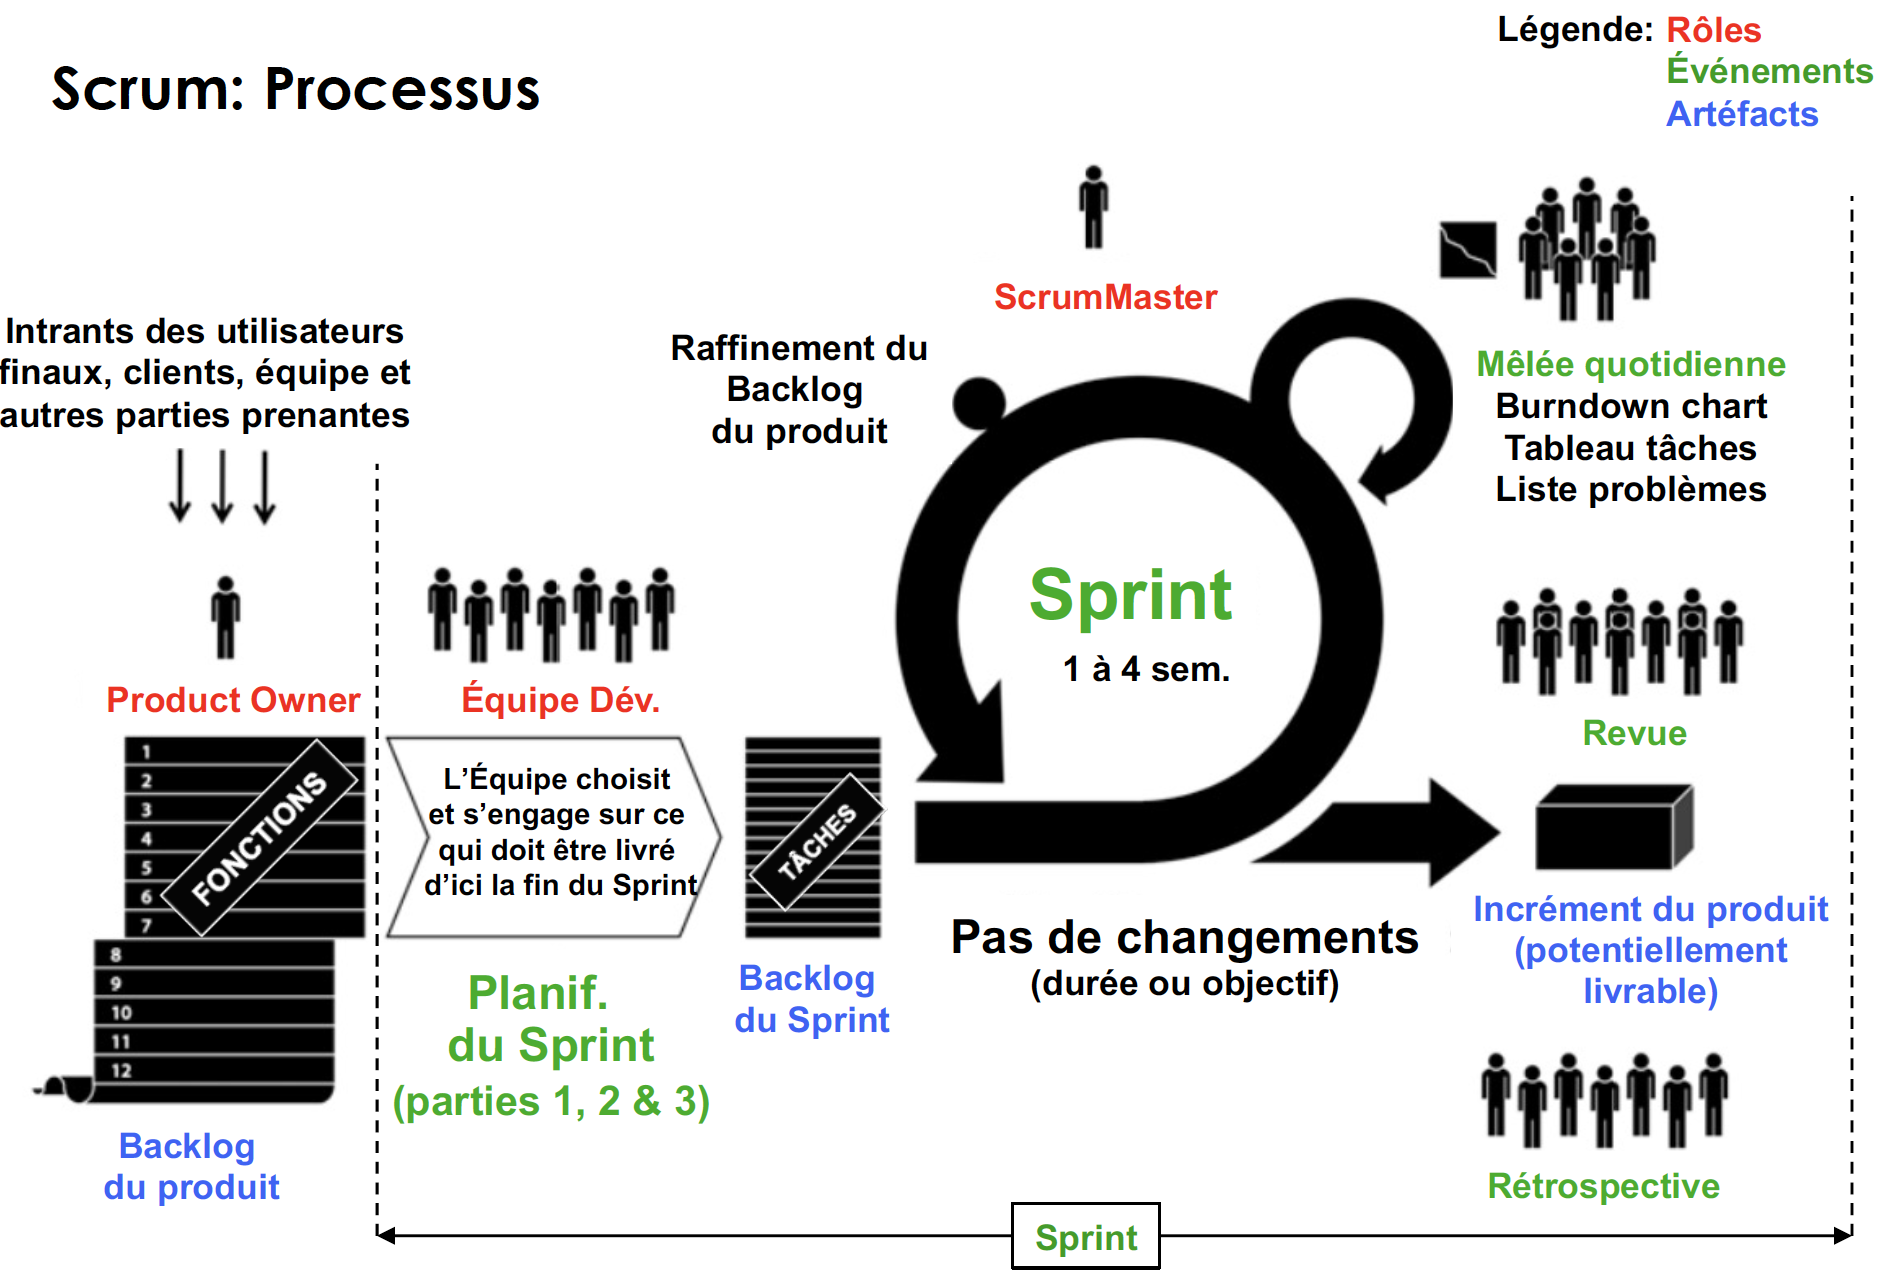
\includegraphics[width=0.8\textwidth,height=\textheight]{images/chapitre8_agilite.png}

}

\caption{\label{fig-scrum}Cycle d'application du processus Scrum, une
approche Agile.}

\end{figure}%

La Figure~\ref{fig-scrum} présente le cycle traditionnel d'application
de l'approche Scrum dans un contexte de travail collaboratif. Dans le
cadre académique, toutes ces composantes peuvent facilement être
adaptées.

Le processus commence par l'organisation d'une « planification de sprint
». Un sprint dure généralement entre une et quatre semaines (dans le
contexte du développement logiciel, une semaine peut être parfois très
utile lorsque les délais sont serrés). Dans le contexte académique, un
sprint de trois ou quatre semaines s'avèrent plus adaptés, voire de 2 ou
3 mois dans le cas d'une rédaction de thèse. Lors de la planification,
toute l'équipe se rencontre quelques heures (généralement 2h ou 3h, en
fonction du nombre de projet en cours et/ou des publications en
rédaction) pour déterminer les grands objectifs qui devront être
réalisés, projet par projet, publication par publication, d'ici la fin
du sprint. Un sprint se conclut toujours par le retour en plénière pour
la planification du sprint suivant. Cette nouvelle planification de
sprint doit désormais, et dorénavant, débuter par une \emph{revue de
sprint}, lors de laquelle les objectifs du sprint terminé sont évalués,
projet par projet, publication par publication, puis par une
\emph{rétrospective}, où les processus cette fois sont évalués. L'équipe
est alors invitée à partager son avis sur la méthode de gestion de
projet, afin d'adapter le processus au contexte particulier et à
renforcer son utilité.

La planification de sprint est menée par le \emph{Scrum Master}, un
membre désigné par l'équipe pour faire le lien entre le \emph{Product
Owner} (dans notre contexte, le ou la directeur/directrice de l'équipe
de recherche) et tous les membres de l'équipe qui travaillent
concrètement sur les projets et publications (les étudiant.e.s, par
exemple). Dans le langage universitaire, le Scrum Master pourrait
représenter le rôle de \emph{coordonnateur}. Il est toutefois recommandé
que le Scrum Master détienne sa certification de Scrum Master, ou ait du
moins suivi sa formation. De nombreuses entreprises offrent des
formations au Québec pour des prix variant entre 1000\$ et 3000\$, pour
2 à 3 jours de formations. La certification, quant à elle, coûte 100\$,
et peut être réalisée via le site Web officiel
\href{https://www.scrum.org/professional-scrum-certifications/professional-scrum-master-assessments}{scrum.org}.
Une formation Agile comme Scrum Master a une énorme valeur sur le marché
de l'emploi. De plus en plus d'entreprises au Québec sont à la recherche
de Scrum Master certifiés, offrant des salaires dépassant les 100 000\$
par année. Comme mentionné en introduction, des compétences en gestion
de projet, mais particulièrement en Agilité, constituent un excellent
moyen d'augmenter rapidement votre valeur dans le milieu universitaire
et sur le marché de l'emploi.

Chaque équipe de projet (il serait normal de compter plusieurs équipes
de projet représentées lors d'un sprint. En fait, il devrait y avoir
autant d'équipes de projet qu'il y a de projet) est dirigée par un.e
\emph{chargé.e de projet}, dont le rôle est de veiller à la coordination
de son équipe. Le.la chargé.e de projet organise les rencontres d'équipe
au besoin, divise les tâches entre les membres, prend la parole lors de
la planification de sprint pour présenter la revue du sprint, et
annoncer les prochains objectifs prévus, qui seront ensuite discutés en
groupe. Quand tous les objectifs pour tous les projets et pour toutes
les publications ont été clairement établis, approuvés par l'ensemble
les membres, en considération du temps que toutes et tous sont
réalistement en mesure d'accorder, puis après avoir déterminé la date de
la prochaine planification de sprint, la séance est levée. Une activité
sociale d'équipe est à ce moment fortement encouragée!

Pour assurer un suivi régulier de l'avancement des objectifs, le Scrum
Master met à l'agenda un ou deux \emph{Scrums} par semaine. Il s'agit de
très courtes rencontres où l'ensemble de l'équipe se retrouve,
idéalement entre 15 et 30 minutes maximum, selon le nombre de projets,
pour répondre à trois questions:

\begin{enumerate}
\def\labelenumi{\arabic{enumi}.}
\tightlist
\item
  Qu'est-ce qui a été fait depuis le dernier scrum?
\item
  Qu'est-ce qui sera fait d'ici le prochain scrum?
\item
  Y a-t-il des blocages?
\end{enumerate}

Tour à tour, le Scrum Master nomme les projets et les publications, dans
leur ordre de priorité, et offre la parole aux chargé.e.s de projet pour
résumer les avancées de leur équipe. Contrairement à la planification de
sprint, le.la directeur/directrice n'a pas besoin d'assister à ces
scrums. Le \emph{Scrum Master} s'assure, si nécessaire, de le.la tenir
informé des bloquants ou des ajustements à mener. Les scrums sont
l'occasion pour l'équipe d'assurer un suivi régulier des
\emph{livraisons} attendues d'ici la fin du sprint.

L'une des caractéristiques fondamentales des méthodes Agiles est le
développement des projets de manière \emph{itérative} et
\emph{incrémentale}. L'itération est le processus répété et cyclique
mené grâce aux sprints. Une équipe Agile est en tout temps en sprint,
jusqu'à la livraison finale du projet ou de la publication (si fin
prévue il y a). Un incrément est la réalisation d'une petite partie dite
« fonctionnelle » du projet, qui peut être soumise à évaluation. Dans le
cadre académique, un incrément peut-être la remise d'une première
version d'une revue de littérature, la réalisation d'une première étape
d'un code R pour l'analyse de données de thèse, le premier jet d'un
devis. Plutôt que d'attendre à la toute fin du processus pour le dépôt
complet d'un projet, une équipe Agile divise son projet en de multiples
itérations, qu'elle soumet pour évaluation à chaque planification de
sprint lors de la phase de la \emph{revue de sprint}. Par une
démonstration, toute l'équipe peut alors constater et discuter du nouvel
incrément proposé, par exemple la présentation de la section
méthodologie d'un article scientifique, et déterminer ensuite les
objectifs du prochain sprint pour la livraison de l'incrément suivant,
disons la collecte de données. Tout projet est ainsi divisé en phase, en
« séquence de développement », d'un sprint à l'autre, de manière
itérative, de sorte à livrer des incréments fonctionnels du projet qui
peuvent être discutés et révisés.

Contrairement aux méthodes traditionnelles, il est essentiel de
comprendre que les méthodes Agiles se nomment « Agile » pour une raison:
elles encouragent la flexibilité. Plutôt que de passer d'un sprint à
l'autre en suivant un plan rigide déterminé des mois, voire des années
auparavant en fonction d'un budget et d'un calendrier coulés dans le
béton, les méthodes Agiles mettent de l'avant le « cycle » de travail,
les \emph{itérations}, qui permettent de revoir le plan, de l'adapter en
cours de route, particulièrement lors de la planification de sprint.
Normalement, lorsque les objectifs de sprint ont été validés par
l'équipe, il n'est pas recommandé de les changer en cours de sprint. Par
contre, de retour en \emph{planif}, chaque membre de l'équipe a son mot
à dire sur la suite; sur ce qui fonctionne bien, sur ce qui devrait être
adapté, toujours avec le projet final en tête.

Pour tout projet ou publication menés seuls, comme la rédaction d'un
mémoire, d'une thèse, ou la création d'un grand album de photos
familiales, ou pour tout besoin de gestion de vie personnelle et
d'objectifs d'avenir, ce processus n'est pas bien différent. Une
personne Agile pourrait, le soir du jour de l'an, mettre sur papier un
certain nombre de résolutions. Elle peut ensuite découper son année en
12 sprints de 4 semaines, et répartir l'accomplissement de ses
résolutions en 12 incréments. Chaque incrément planifié doit être
réaliste et faire avancer, petit à petit, les objectifs vers la
livraison finale, à la fin de l'année. Une fois aux quatre semaines,
cette personne peut prendre un moment seul de \emph{planification de
sprint} pour faire la \emph{revue} des quatre dernières semaines et
réviser les objectifs à atteindre pour les quatre semaines suivantes.

Comme on l'a vu, l'Agile ne s'applique pas uniquement au monde du
développement logiciel, voire à une grande équipe académique. Elle est
d'abord et avant tout une philosophie, possible d'être menée, réfléchie
et appliquée à son quotidien.

L'efficacité et les nombreuses possibilités qu'offre cette méthode ont
généré, bien entendu, un marché très lucratif d'outils numériques. La
section suivante présentera les leaders du marché, et offrira des
instructions sous forme de conseils pour l'utilisation adaptée de ces
outils, notamment par la création de \emph{stories} à l'intérieur d'un
tableau \emph{Kanban}.

\subsection{Arpentage et choix éditorial: pourquoi utiliser un outil de
gestion de
projet}\label{arpentage-et-choix-uxe9ditorial-pourquoi-utiliser-un-outil-de-gestion-de-projet}

Tous les outils numériques de gestion de projets actuels (ou presque)
sont conçus sur les enseignements des méthodes Agiles. Pour le contexte
académique, ce chapitre propose en premier lieu l'application de
l'approche Scrum, détaillé précédemment. Une seconde approche Agile, la
méthode (et l'outil) Kanban, se combine aisément et efficacement à
l'approche Scrum et au travail scientifique. Le Kanban est l'outil par
excellence mis de l'avant dans les très populaires logiciels de gestion
de projet \emph{Trello}, \emph{Jira}, \emph{Monday}, \emph{Asana} et
\emph{Notion} (cette liste n'est pas limitative. À ce jour, il existe
des dizaines de logiciels de gestion de projets tout aussi populaires
les uns que les autres comme \emph{ClickUp}, \emph{Wrike},
\emph{Basecamp}, et même la plateforme de communication \emph{Slack},
qui propose depuis 2024 sa solution de gestion de projet pour répondre
aux attentes en gestion de projet de ses clients).

Offert de base dans tous les outils numériques nommés ci-dessus, le
Kanban permet d'intégrer et de visualiser, dans un tableau comptant au
minimum 3 colonnes (« À faire », « En cours », « Terminé »), les «
tâches » à réaliser dans une échéance pour avancer la réalisation des
objectifs de sprint. En Agilité, une tâche est nommée \emph{Story}. Une
story est un livrable, un morceau du projet (le « quoi »), pris en
charge volontairement ou délégué à un membre de l'équipe par le.la
chargé.e de projet. On utilise le terme story pour distinguer de la
rapide tâche; une story peut quelques fois comporter plusieurs tâches
(le « comment »).

Voici un exemple d'application de tous les concepts Agile vu jusqu'à
présent. Dans le milieu académique, un \emph{projet} pourrait être la
création d'une étude scientifique. La création de cette étude pourrait
être divisée en dix \emph{sprints} de quatre semaines, présentant ainsi
dix \emph{livrables} clairs qui permettent un suivi en planification de
sprint (bien sûr, certaines études peuvent prendre des années à aboutir.
Certaines collectes de données sont plus longues, mais là n'est pas le
point: toute étude menée en gestion de projet Agile peut être réfléchie
d'emblée en fonction de son contexte et de ses objectifs, et être
divisée en un nombre logique et réaliste de sprints, que ce soit 5 ou
15):

\begin{itemize}
\tightlist
\item
  1er sprint: Idéation et structuration d'une question de recherche;
\item
  2e sprint: Première version d'une revue de littérature;
\item
  3e sprint: Rédaction du devis, choix théoriques, enregistrement des
  hypothèses, demande éthique;
\item
  4e sprint: Préparation méthodologique, raffinement de la revue de
  littérature;
\item
  5e sprint: Collecte des données;
\item
  6e sprint: Analyse des données;
\item
  7e sprint: Rédaction des résultats;
\item
  8e sprint: Rédaction de l'étude complète (introduction, discussion);
\item
  9e sprint: Révision du texte;
\item
  10e sprint: Soumission.
\end{itemize}

En divisant un projet de cette manière, les ressources nécessaires
peuvent être réfléchies et réparties à l'avance (par exemple: il faudra
engager deux auxiliaires de recherche pour la collecte de données du 5e
sprint). Tous les objectifs de sprint deviennent évidents et
prévisibles, et chaque story peut être rédigée pour accomplir ces
objectifs.

Un outil numérique comme \emph{Notion} peut ensuite être utilisé pour
créer et remplir un Kanban, qui se compose de quatre colonnes:

\begin{enumerate}
\def\labelenumi{\arabic{enumi}.}
\tightlist
\item
  \textbf{À venir}: c'est le \emph{backlog} (le « registre des tâches »)
  du projet. Toutes les stories qui seront à réaliser lors de sprints
  futurs s'y trouvent déjà, en ordre, de sorte à visualiser le travail «
  à venir »;
\item
  \textbf{À faire}: c'est le \emph{backlog} du sprint. Toutes les
  stories qui sont à réaliser à l'intérieur du sprint en cours s'y
  trouvent, avec une date d'échéance et une assignation;
\item
  \textbf{En cours}: Quand une story du sprint est engagée, le membre de
  l'équipe à qui elle est assignée doit la déplacer dans cette colonne,
  pour signaler son avancement;
\item
  \textbf{Terminé}: Toutes les stories du sprint en cours qui sont
  accomplies y apparaissent.
\end{enumerate}

\begin{figure}

\centering{

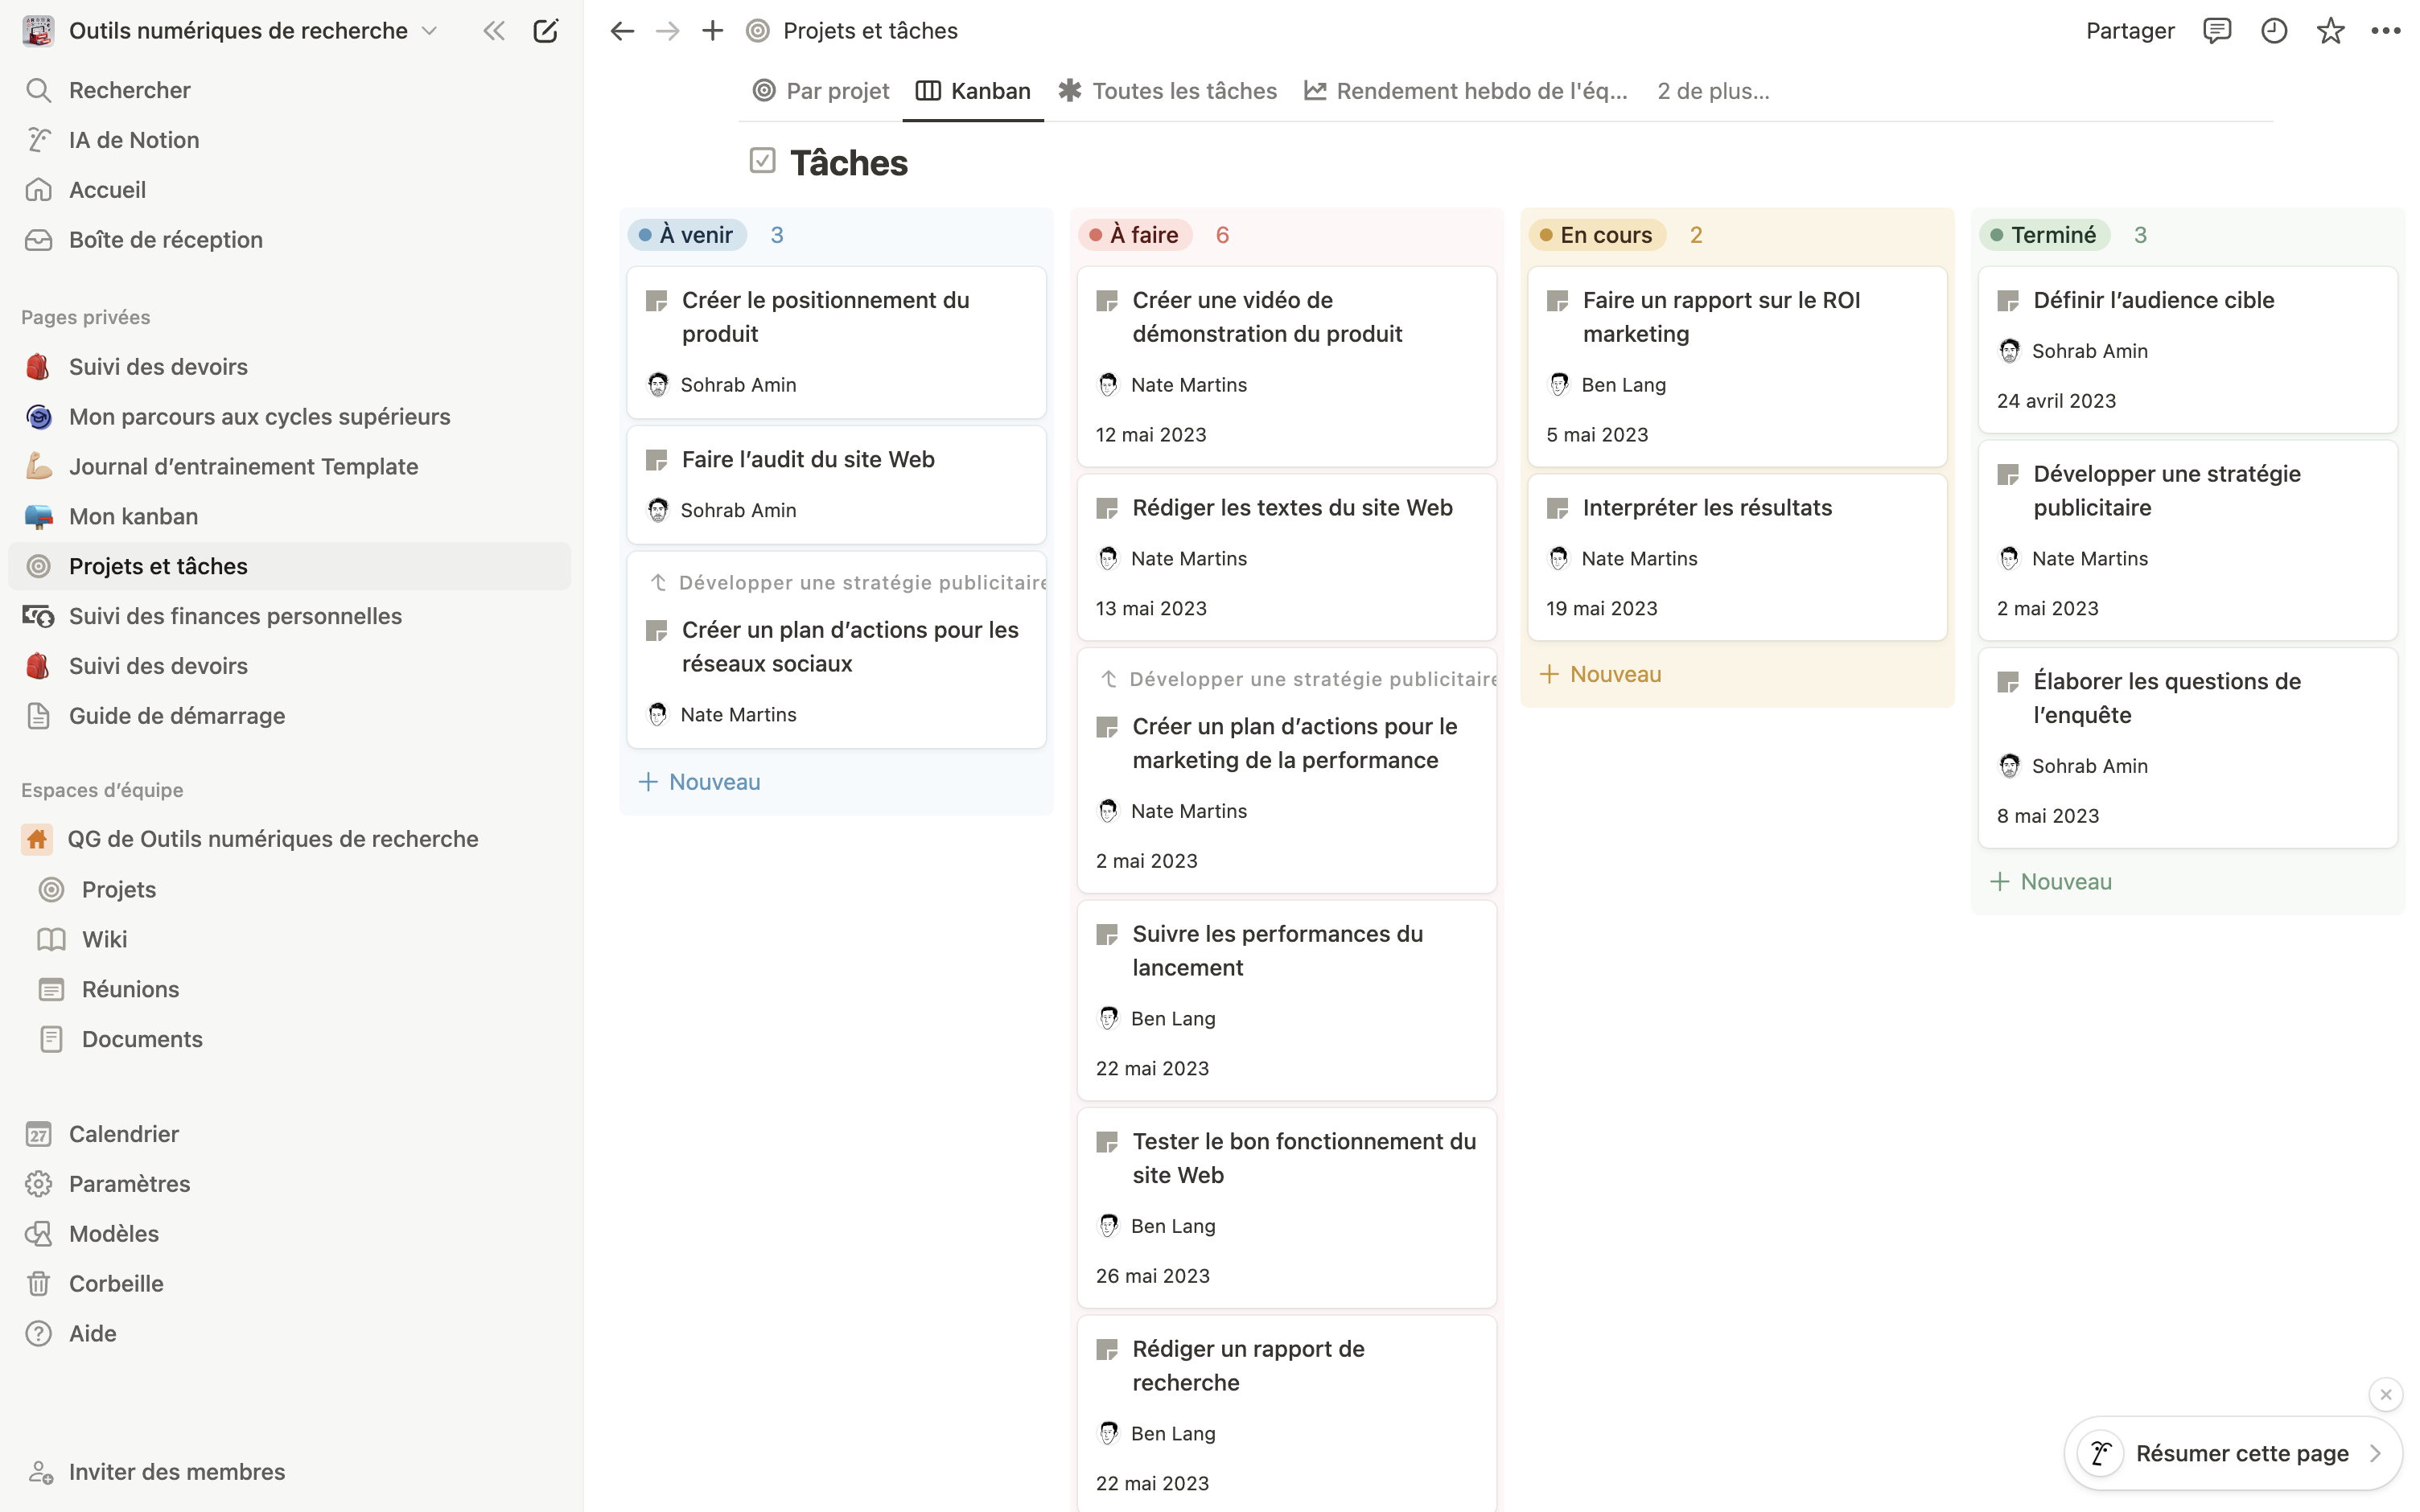
\includegraphics{images/chapitre8_kanban_notion.png}

}

\caption{\label{fig-kanban}L'outil de gestion de projet Notion propose
d'emblée des modèles de Kanban pour la création et le suivi des
stories.}

\end{figure}%

En sortant de la première planification de sprint, l'équipe de recherche
se retrouve face à des objectifs clairs, réalistes, divisés en stories
rédigées dans un Kanban bien rempli. Ne reste plus qu'à se mettre à la
tâche, et à se retrouver lors des scrums hebdomadaires pour assurer le
suivi.

À la fin du sprint, lors de la rencontre de planification du sprint
suivant, une équipe Agile débute toujours par la \emph{revue de sprint},
qui permet de s'assurer que toutes les stories qui avaient été
déplacées, il y a quatre semaines, de la colonne « À venir » à « À faire
», se trouvent désormais dans « Terminées ». Grâce à la réalisation de
toutes les stories, les objectifs de sprint devraient être considérés
comme accomplis. Il est maintenant temps de se préparer à l'atteinte des
objectifs du sprint suivant, en vidant la colonne « Terminé », puis en
déplaçant les stories du sprint suivant, qui étaient dans « À venir »,
dans « À faire » en leur ajoutant une échéance et une assignation. Le
cycle peut alors recommencer. Une itération est terminée, un incrément
du projet a été livré, et une nouvelle phase de développement est prête
à être lancée.

En mélangeant de cette manière les approches Agile \emph{Scrum} et
\emph{Kanban}, on obtient tout simplement l'approche \emph{Scrumban}!

Comme mentionné, tous les outils numériques sur le marché (ou presque)
proposent actuellement les éléments nécessaires à la mise en place d'une
gestion de projet \emph{Scrumban}. En 1984, la sortie de \emph{Microsoft
Project} est une révolution en gestion de projet. La première version
disponible sur Windows en 1990 permet enfin aux chefs de projet
d'utiliser un outil numérique de planification pour gérer des tâches,
visualiser les étapes de développement dans des diagrammes de Gantt,
suivre la gestion des coûts et des ressources, et extraire l'ensemble
des données pour produire des analyses et des rapports d'avancement de
projet. À l'ère des méthodes traditionnelles, \emph{Microsoft Project}
domine le marché, et poursuit sa domination bien au-delà, étant toujours
le \#1 mondial en 2011, utilisé par plus de 20 millions d'utilisateurs.
À l'ère de l'Agilité, les solutions de \emph{Microsoft} pour la gestion
de projet existent toujours, mais ne s'adressent plus uniquement aux
chefs d'équipe. \href{https://tasks.office.com/}{\emph{Microsoft
Planner}}, sorti en 2015, est la proposition plus simple de
\emph{Microsoft} pour le travail d'équipe qui se compare davantage aux
applications numériques visuelles, flexibles et extrêmement populaires
ayant fait irruption sur le marché depuis 2010. En croisant
\href{https://www.microsoft.com/fr-ca/microsoft-365/project/agile-methodology}{ses
outils de gestion de projet et l'outil de communication \emph{Teams}},
\emph{Microsoft} permet à tous les membres d'une équipe de gérer et
suivre l'évolution de leur travail de manière Agile. Pour les
utilisateurs des services \emph{Microsoft}, cette solution intégrée peut
être très avantageuse, avec un faible coût d'apprentissage.

Longtemps seule et dominante dans le marché, \emph{Microsoft}
compétitionne aujourd'hui avec une multitude d'acteurs. Les premières
plateformes collaboratives comme \emph{Basecamp} (1999) et \emph{Jira}
(2002) marquent le début du suivi en ligne, permettant aux équipes de
travailler à distance, en temps réel, et de suivre leur progression de
manière Agile. Développé par la compagnie \emph{Atlassian}, \emph{Jira}
se concentre particulièrement sur la gestion des suivis de \emph{bugs},
d'incidents et de projets au niveau « macro », par le suivi des
\emph{sprints}, des \emph{objectifs de sprint} et des \emph{backlog}.
L'application est intégrée à \emph{Google Workspace} en 2021, et évolue
en parallèle à \emph{Trello}, un autre outil de gestion de projet en
ligne lancé par \emph{Atlassian} en 2011 et concentré sur le Kanban
utilisateur, pour le suivi « micro » des tâches. Les différences sont
légères avec les applications \href{https://asana.com/}{\emph{Asana}}
(2008) et \href{monday.com}{\emph{monday.com}} (2012), toutes basées
principalement sur le développement et le suivi de projets Agiles via
des vues de tâches en tableau Kanban, en calendrier, voire en Gantt (le
diagramme de Gantt, même à l'ère de l'Agilité, demeure toujours très
populaire).

Des propositions de logiciels libres \emph{open source} sont bien sûr
présentes en ligne.
\href{https://www.openproject.org/}{\emph{OpenProject}} (2012) et
\href{https://taiga.io/}{\emph{Taiga}} (2014) sont des outils Agiles
présentant tous les avantages liés aux logiciels libres tels que la
gratuité du service et la possibilité de modification et de
redistribution.

\begin{table}
\centering
\begin{talltblr}[         %% tabularray outer open
caption={Résumé des principaux outils de gestion de projet},
]                     %% tabularray outer close
{                     %% tabularray inner open
width={0.75\linewidth},
colspec={X[]X[]X[]X[]X[]},
}                     %% tabularray inner close
\toprule
Critères & Microsoft & monday.com & OpenProject & Notion \\ \midrule %% TinyTableHeader
Accessibilité (Gratuit ou peu dispendieux) & Payant & Payant & Gratuit (logiciel libre) & Utilisation de base gratuite \\
Existence d'une communauté d'utilisateurs & Oui & Limitée & Limitée & Oui \\
Popularité dans le champ & Oui & Non & Non & Oui \\
Compatibilité avec d'autres outils & Avec les outils Microsoft & Oui & Oui & Oui \\
Transparence et réplicabilité & Non & Non & Oui & Non \\
Adaptabilité et flexibilité & Non & Non & Oui & Oui \\
\bottomrule
\end{talltblr}
\end{table}

\subsection{Manuel d'instruction: Notion pour la vie professionnelle et
personnelle}\label{manuel-dinstruction-notion-pour-la-vie-professionnelle-et-personnelle}

En août 2024, \href{https://www.notion.so/fr}{\emph{Notion}} dépasse la
barre du 100 millions d'utilisateurs. Juste avant la pandémie de
COVID-19, \emph{Notion} atteignait son premier million. En l'espace de
quelques années, l'outil a rejoint, voire dépassé ses concurrents. Une
popularité incontestable, notamment due à sa grande flexibilité.

Créé en 2013 par Ivan Zhao et Simon Last, \emph{Notion} se présente
comme un outil de gestion de projet « tout-en-un », offrant à
l'utilisateur des pages blanches qu'il doit lui-même remplir en fonction
de ses besoins. Les pages peuvent intégrer du texte, des bases de
données, des images, des vidéos, des PDF, des liens Web, et bien plus.
Chaque page peut ainsi devenir un outil de documentation, ou un tableau
Kanban rempli de stories, ou des notes de rencontres, ou un calendrier
des livrables de sprint. Il importe à l'utilisateur de connaitre ses
besoins, et d'être créatif.

Cette liberté peut représenter un défi. Il est nécessaire d'avoir
l'esprit « architecte » pour apprécier \emph{Notion.} En comparaison,
\emph{monday.com} ou \emph{Trello} offrent un cadre de travail déjà
défini et balisé à l'utilisateur. Les instructions à l'entrée sont
claires: l'utilisateur a un Kanban à remplir, et il peut facilement
faire le suivi de ses tâches.

Sur \emph{Notion}, tout (ou presque) est possible. Notion possède
d'ailleurs \href{https://www.notion.so/fr/help/formulas}{son propre
langage de programmation} pour coder des fonctions originales dans des
bases de données.

Il n'est toutefois pas nécessaire d'aller dans la complexité: sans être
un logiciel libre, \emph{Notion} offre la possibilité à ses utilisateurs
de créer leur propre « modèle », et de les offrir (voire de les vendre,
si désiré!) à la communauté Web. Ainsi,
\href{https://www.notion.so/fr/templates}{plus de 20 000 modèles
\emph{Notion} sont disponibles en ligne}! Vous trouverez de multiples
modèles pour répondre à tous vos besoins: que ce soit pour la gestion de
vos finances ou pour gérer votre vie étudiante, la communauté
\emph{Notion} est large et structurée. Tous les modèles disponibles
s'importent en deux clics, et vous permettent de les modifier
complètement au besoin. Avec le temps et l'expérience, vous pourrez
vous-même créer vos propres modèles et les offrir gratuitement (ou à
votre prix!) à la communauté.

Notez également que l'utilisation individuelle de \emph{Notion} est tout
à fait gratuite. En payant, vous vous offrez bien sûr davantage de
possibilités (comme l'utilisation de l'intelligence artificielle
intégrée de \emph{Notion}), mais l'utilisation gratuite de base peut
être bien suffisante pour vos besoins.

Avec un seul outil, \emph{Notion} peut vous permettre de gérer à la fois
votre vie personnelle et votre vie professionnelle. Pour se lancer,
\href{https://www.notion.so/fr/help/category/new-to-notion}{des guides
simples sont disponibles (en français!) sur le site Web}.

Notez également que \emph{Notion} possède sa propre application de
calendrier. \emph{Notion Calendar} permet d'importer vos calendriers
\emph{Google}, en plus d'afficher tous les jours vos échéances de
stories.

Vous souhaitez créer une page \emph{Notion} pour votre prochain voyage
entre amis? Rien de plus simple! Vous pourrez y intégrer une liste
d'idées d'activités, un calendrier de vos destinations, un Kanban
rassemblant toutes les tâches à accomplir d'ici au départ, et partager
le tout à vos amis via le Web. En deux clics, toutes les pages
\emph{Notion} peuvent être transformées en site Web consultable et
modifiable (si on le souhaite et l'autorise).

Depuis son lancement, \emph{Notion} est en constante évolution.
Impossible de savoir à quoi ressemblera l'application dans 10 ans.
Victime de son succès, l'entreprise s'est plusieurs fois réinventée,
misant sur une gestion de projet Agile, en communication avec sa
clientèle, pour développer un outil à l'image des besoins et des
intérêts de ses utilisateurs.

\section{Les outils de gestion de
données}\label{les-outils-de-gestion-de-donnuxe9es}

\subsection{Arpentage et choix éditorial: pourquoi utiliser Git, GitHub
et
Dropbox}\label{arpentage-et-choix-uxe9ditorial-pourquoi-utiliser-git-github-et-dropbox}

Lorsque l'on aborde le domaine de la recherche scientifique en sciences
sociales numériques, la collaboration et la gestion efficace du code
deviennent des éléments cruciaux pour progresser dans ses projets. Dans
cette optique, les outils de gestion de versions décentralisés ont pris
une place prépondérante. Parmi eux, Git et GitHub se démarquent tant par
leur popularité que par leur efficacité.

Git, développé par Linus Torvalds en 2005, s'est imposé comme le système
de gestion de versions décentralisé de référence. Avec l'essor des
projets logiciels dans les décennies précédentes, un besoin s'est créé
pour suivre l'évolution des fichiers de code au fil du temps. Quand
plusieurs centaines de développeurs travaillent sur un même projet, ce
suivi est essentiel pour éviter les conflits entre les versions. Bien
que des systèmes centralisés existaient pour ce type de gestion, Git se
distingue par sa décentralisation : chaque développeur détient une copie
complète du projet, incluant toutes les modifications passées. Cela
permet aux équipes de travailler de manière indépendante, sans dépendre
d'un serveur central, ce qui réduit les risques de conflits. Sa
principale force réside dans sa capacité à suivre l'évolution d'un
projet en enregistrant les modifications du code source. Chaque
modification, ou commit, est enregistrée avec un message explicatif et
un identifiant unique, permettant aux collaborateurs de comprendre
facilement les évolutions du projet et d'assurer l'intégrité des
données.

GitHub, lancé en 2008, est né pour répondre aux besoins de collaboration
croissants dans le monde du développement open source. Avant GitHub, les
développeurs pouvaient utiliser Git en local pour gérer les versions,
mais il manquait un espace centralisé pour partager le code et
coordonner les efforts. GitHub a donc apporté cette solution en
intégrant Git à une plateforme web, où les développeurs pouvaient
héberger leurs dépôts, collaborer, et suivre le développement en ligne.
Ce qui distingue GitHub, c'est son aspect social : les fonctionnalités
comme les \emph{pull requests}, les gestionnaires de problèmes, et le
suivi des modifications permettent aux équipes de travailler
efficacement et d'interagir facilement autour du code. Cette combinaison
d'outils a transformé GitHub en un espace incontournable pour les
projets open source, facilitant le partage des connaissances et la
collaboration.

Git et GitHub incarnent efficacement l'évolution vers des méthodes de
travail plus flexibles, collaboratives et transparentes. Grâce à leur
capacité de gestion de versions et d'historique des modifications, ils
permettent aux chercheurs d'embrasser une philosophie Agile en assurant
un suivi minutieux des changements, facilitant ainsi l'itération rapide
et la reproductibilité des projets.

En sciences sociales numériques, où le partage et la collaboration sont
essentiels, Git et GitHub offrent plusieurs avantages majeurs. Tout
d'abord, ils permettent de suivre les modifications apportées au texte
ou au code, ce qui facilite la reproductibilité des résultats. Les
chercheurs peuvent revenir à n'importe quelle version précédente de leur
projet, une fonctionnalité particulièrement utile pour corriger des
erreurs ou analyser l'impact de différentes approches. Lorsqu'un projet
est initialisé avec Git, un dossier caché appelé .git est créé dans le
répertoire. Ce dossier contient tout l'historique des modifications
apportées, y compris les informations sur chaque \emph{commit}, sur les
différentes « branches » créées (versions parallèles du projet) et sur
les métadonnées associées. Ainsi, même en travaillant avec plusieurs
collaborateurs, chacun peut voir quels changements ont été effectués,
par qui et pourquoi, tout en s'assurant qu'aucune version de leur
travail ne soit perdue.

Git et GitHub favorisent le travail collaboratif. Plusieurs chercheurs
peuvent travailler sur le même projet simultanément, chacun dans sa
branche de développement. Une fois les modifications effectuées, il est
possible de fusionner les branches (encore une fois, comprendre ici les
différentes « versions ») pour intégrer les changements. Cette approche
évite les conflits majeurs. Un conflit survient lorsque deux
collaborateurs modifient et enregistrent le même fichier ou la même
partie de texte de manière indépendante, comme cela peut arriver dans un
dossier Dropbox partagé. Ainsi, contrairement aux outils classiques
comme Microsoft Word, où deux personnes peuvent se retrouver avec des
versions distinctes d'un même document et perdre beaucoup de temps à
fusionner manuellement les modifications, Git identifie automatiquement
les zones conflictuelles et aide à les résoudre de façon plus
méthodique.

Bien qu'il existe plusieurs alternatives à l'utilisation combinée de Git
et de GitHub sur le marché, ces deux plateformes liées continuent de
dominer le domaine de la gestion de versions décentralisée. Parmi les
alternatives notables, on peut citer Mercurial, Bitbucket, GitLab et
SourceForge. Chacun de ces outils offre des fonctionnalités similaires à
celles de Git et GitHub.

Github n'est pas un logiciel libre, mais il est gratuit pour ses
fonctionnalités essentielles, et est abondamment utilisé pour y déposer
des codes sources ouverts. Cela permet aux chercheurs en sciences
sociales numériques de partager leurs textes et leurs codes avec la
communauté académique et de bénéficier des contributions d'autres
chercheurs. Cela favorise un environnement de partage des connaissances
et de collaboration fructueuse. Cependant, Git et GitHub ne sont pas
sans leurs défis. La courbe d'apprentissage peut être raide pour les
débutants, car ces outils impliquent des concepts spécifiques tels que
les branches, les conflits de fusion et les \emph{pull requests}. Voici
un résumé des avantages de Git et Github :

\begin{enumerate}
\def\labelenumi{\arabic{enumi}.}
\item
  \emph{Intégration et adoption répandue}~: Git est devenu un standard
  de facto dans l'industrie du développement logiciel. Sa popularité et
  son adoption répandue signifient que de nombreuses ressources
  d'apprentissage, des tutoriels et des forums de support sont
  disponibles en ligne, ce qui facilite l'utilisation de cet outil pour
  les chercheurs en sciences sociales débutants. GitHub, en tant que
  plateforme principale de gestion des versions, bénéficie également
  d'une grande base d'utilisateurs et d'une communauté active, ce qui
  encourage la collaboration et le partage des connaissances.
\item
  \emph{Facilité de collaboration}~: Git et GitHub sont conçus pour
  faciliter la collaboration entre les individus et les équipes. Les
  chercheurs en sciences sociales travaillent souvent ensemble sur des
  projets de recherche, et la capacité de suivre les modifications, de
  gérer les conflits et de fusionner les contributions devient
  essentielle. L'interface conviviale de GitHub, avec des
  fonctionnalités telles que les demandes de fusion et les commentaires
  en ligne, simplifie grandement la collaboration.
\item
  \emph{Suivi des versions et recherche reproductible}~: Les chercheurs
  en sciences sociales doivent s'assurer que leurs travaux sont
  reproductibles et vérifiables. Git permet de suivre les versions du
  code, ce qui signifie que les chercheurs peuvent retrouver facilement
  des versions antérieures pour reproduire des analyses spécifiques ou
  corriger des erreurs. Cette fonctionnalité est cruciale pour maintenir
  l'intégrité des résultats de recherche.
\item
  \emph{Infrastructure et sécurité}~: GitHub offre une infrastructure
  robuste pour l'entreposage sécurisé des dépôts Git. Les chercheurs
  peuvent être assurés que leurs travaux sont sauvegardés et protégés
  contre les pertes de données accidentelles. De plus, les contrôles
  d'accès et les autorisations granulaires de GitHub permettent aux
  chercheurs de contrôler qui peut accéder et contribuer à leurs
  projets.
\end{enumerate}

En somme, Git et GitHub offrent aux chercheurs en sciences sociales
numériques un moyen puissant de gérer leur code, de collaborer
efficacement et de contribuer à la communauté académique grâce à l'open
source. Bien que leur apprentissage puisse représenter un défi initial,
les avantages qu'ils apportent en termes de suivi des versions, de
collaboration et de partage des connaissances en font des outils
essentiels dans l'arsenal de tout chercheur moderne.

Bien que Git et GitHub soient des outils puissants pour la gestion de
versions et l'entreposage de code, ils ne sont pas conçus pour stocker
et partager de larges volumes de données brutes. En effet, la gestion
des fichiers volumineux ou des bases de données complexes peut
rapidement devenir problématique dans ces environnements. C'est là que
les services infonuagiques entrent en jeu.

Dans le cadre de la recherche académique en sciences sociales, la
gestion des données occupe une place cruciale. La manière dont vous
entreposez, gérez, et partagez vos données peut avoir un impact direct
sur la sécurité, la confidentialité, et la reproductibilité de vos
recherches. Que ce soit pour des données quantitatives, des résultats
d'enquêtes ou des transcriptions d'entretiens, les outils de gestion de
données permettent de centraliser, sécuriser et organiser les fichiers
tout en facilitant la collaboration avec d'autres chercheurs.

Aujourd'hui, les chercheurs manipulent une quantité croissante de
données. L'accès facile aux fichiers, la possibilité de les partager
rapidement avec des collègues et la sauvegarde automatique sont devenus
des impératifs dans la gestion de projet. De plus, dans un environnement
où la collaboration à distance est omniprésente, la gestion efficace des
données permet de maintenir un haut niveau de productivité et de
transparence dans les travaux de recherche.

Lorsqu'il s'agit d'entreposer vos données de recherche, la règle d'or
est de ne jamais perdre d'informations précieuses. Cette préoccupation
prend toute son importance lorsqu'un chercheur en sciences sociales,
seul ou en équipe restreinte, se lance dans un projet. Pour répondre à
ce besoin, les services d'entreposage infonuagiques se révèlent
indispensables. Voici quelques avantages d'un entreposage sur le nuage
pour la recherche~:

\begin{enumerate}
\def\labelenumi{\arabic{enumi}.}
\item
  \emph{Sécurité des données} : Que vous travailliez avec des données
  sensibles ou non, la sécurité est essentielle pour protéger
  l'intégrité de vos fichiers. De bons outils garantissent que vos
  données ne sont pas exposées à des risques tels que des piratages ou
  des pertes accidentelles.
\item
  \emph{Collaboration et partage} : En particulier dans le cadre de
  collaborations interinstitutionnelles, il est indispensable d'avoir
  des outils qui permettent de partager facilement des fichiers avec vos
  collègues, où qu'ils se trouvent.
\item
  \emph{Sauvegarde et versionnage} : Une bonne gestion des données
  permet de garder des copies de sauvegarde de vos fichiers et de suivre
  l'historique des versions, vous offrant la possibilité de revenir à
  une version antérieure si nécessaire.
\end{enumerate}

Pour répondre aux besoins variés des chercheurs, des dizaines d'outils
de gestion de données ont émergé. Nous allons ici comparer quatre
d'entre eux : Dropbox, Google Drive, Nextcloud, et Microsoft OneDrive.

Dropbox est très utilisé dans plusieurs milieux, même à titre
d'utilisation personnelle. Dans le milieu académique, le partage de
fichiers peu volumineux par Dropbox est très fréquent. Son utilisation
est relativement accessible : 2 Go sont offerts gratuitement, puis un
abonnement est nécessaire pour entreposer d'avantage. Dropbox se
démarque par sa popularité et par son interface intuitive, s'intégrant
facilement dans le gestionnaire de fichiers. Bien que ce soit simple
d'utilisation, Dropbox ne permet pas une grande flexibilité et
réplicabilité dès qu'il y a un besoin plus important pour des données à
gros volume ou plus sensible. Dropbox est ainsi très utile dans le cadre
de gestion de données collaborative relativement simple.

Google Drive est très facile d'utilisation par son intégration au sein
des outils Google. La plateforme, en générale, est fréquemment utilisée
dans le cadre de rédaction, pour son suivi des modifications et la
possibilité de travailler à plusieurs sur un document en même temps.
Google Drive offre 15 Go gratuits, et son utilisation est simple et
intuitive. Cependant, son utilisation en local n'est pas très adaptée.
Il nécessite souvent une interaction via son interface web pour le
téléchargement ou le partage de fichiers. Si vous codez des analyses
statistiques et manipulez des jeux de données en R, par exemple, Google
Drive est peu adapté pour la sauvegarde de jeux de données directement
dans votre arborescence.

Microsoft OneDrive Fait partie de la suite Microsoft 365. C'est donc un
choix judicieux pour les utilisateurs des outils Microsoft, pour leur
compatibilité. Comme Dropbox, OneDrive permet la sauvegarde de fichiers
en local, ce qui facilité son utilisation pour l'entreposage de fichiers
manipulés avec un language de programmation. OneDrive est généralement
perçu comme étant moins simple et rapide pour sa synchronisation que
Dropbox, mais sa valeur de centralisation est indégnable si la suite
Microsoft est employée.

Nextcloud est une plateforme de stockage libre d'accès qui se distingue
par sa flexibilité et son contrôle personnalisé. Contrairement à des
services comme Dropbox, Nextcloud permet aux utilisateurs d'héberger
leurs fichiers eux-mêmes, ce qui garantit une meilleure sécurité et
confidentialité des données. C'est idéal pour les chercheurs qui veulent
un accès libre et plus de contrôle sur leurs données. Cependant,
Nextcloud nécessite plus de compétences techniques pour l'installation
et la gestion, ce qui peut être un obstacle pour ceux qui recherchent
une solution ``clé en main''.

\begin{table}
\centering
\begin{talltblr}[         %% tabularray outer open
caption={Résumé des principaux outils de gestion de données},
]                     %% tabularray outer close
{                     %% tabularray inner open
width={0.75\linewidth},
colspec={X[]X[]X[]X[]X[]},
}                     %% tabularray inner close
\toprule
Critères & Dropbox & Google Drive & OneDrive & Nextcloud \\ \midrule %% TinyTableHeader
Accessibilité (Gratuit ou peu dispendieux) & Limitée - Abonnement mensuel & Oui & Limitée & Oui - Si auto-hébergé \\
Existence d'une communauté d'utilisateurs & Oui & Oui & Oui & Oui \\
Popularité dans le champ & Oui & Oui & Limitée & Limitée \\
Compatibilité avec d'autres outils & Oui & Avec les outils Google & Avec les outils Microsoft & Oui, avec configuration \\
Transparence et réplicabilité & Limitée & Moyenne & Moyenne & Oui \\
Adaptabilité et flexibilité & Limitée & Oui & Moyenne & Très flexible \\
\bottomrule
\end{talltblr}
\end{table}

\subsection{Manuel d'instructions: comment utiliser Git, Github et
Dropbox}\label{manuel-dinstructions-comment-utiliser-git-github-et-dropbox}

Pour utiliser Git et GitHub efficacement dans un contexte de recherche
en sciences sociales numériques, il est recommandé de suivre quelques
bonnes pratiques. Tout d'abord, il est important de structurer son
répertoire Git de manière logique, en organisant les fichiers et les
dossiers de manière cohérente. Les messages de \emph{commit} doivent
être descriptifs et clairs, pour permettre à tous les collaborateurs de
comprendre les changements effectués.

Il est également conseillé de travailler sur des branches distinctes
pour chaque fonctionnalité majeure. Cela facilite la gestion des
changements et minimise les conflits lors de la fusion. Les chercheurs
devraient également consulter régulièrement les projets et les problèmes
sur GitHub pour encourager une communication ouverte et résoudre
rapidement les problèmes.

Dans le contexte de la recherche en sciences sociales numériques, la
gestion efficace du code, la collaboration transparente et la
préservation des données sensibles sont des impératifs. Imaginons que
vous êtes un jeune chercheur en sciences sociales qui étudie l'impact
des médias sur l'opinion publique. Vous utilisez le langage de
programmation R pour analyser des données de médias et des données de
sondage. Bien que vous travailliez seul, vous souhaitez rendre votre
travail accessible à votre équipe pour validation et permettre à vos
collègues de contribuer aux améliorations. Voici comment vous pouvez
utiliser Git et GitHub pour gérer votre projet de manière structurée et
collaborative.

Étape 1~: Création d'un répertoire local et initialisation de Git

Ouvrez votre terminal (sur MacOS et Linux) ou l'application Git Bash
(sur Windows) et naviguez vers le dossier où vous souhaitez enregistrer
votre projet.

\begin{Shaded}
\begin{Highlighting}[]
\BuiltInTok{cd}\NormalTok{ chemin/vers/votre/dossier}
\end{Highlighting}
\end{Shaded}

Créez un nouveau répertoire pour votre projet et accédez-y.

\begin{Shaded}
\begin{Highlighting}[]
\FunctionTok{mkdir}\NormalTok{ mon\_projet}
\end{Highlighting}
\end{Shaded}

\begin{Shaded}
\begin{Highlighting}[]
\BuiltInTok{cd}\NormalTok{ mon\_projet}
\end{Highlighting}
\end{Shaded}

Initialisez Git dans ce répertoire.

\begin{Shaded}
\begin{Highlighting}[]
\FunctionTok{git}\NormalTok{ init}
\end{Highlighting}
\end{Shaded}

Étape 2~: Ajout de votre code et de vos fichiers

Ajoutez vos fichiers R contenant le code pour l'analyse des médias et
des sondages dans le répertoire. Par exemple, vous pouvez avoir des
fichiers \emph{analyse\_medias.R} et \emph{analyse\_sondages.R}.

Utilisez la commande \texttt{git\ status} pour vérifier l'état de vos
fichiers.

\begin{Shaded}
\begin{Highlighting}[]
\FunctionTok{git}\NormalTok{ status}
\end{Highlighting}
\end{Shaded}

Étape 3~: Ajout, validation et dépôt de vos modifications

Ajoutez vos fichiers pour qu'ils soient prêts à être validés.

\begin{Shaded}
\begin{Highlighting}[]
\FunctionTok{git}\NormalTok{ add }\AttributeTok{{-}A}
\end{Highlighting}
\end{Shaded}

Validez vos modifications avec un message descriptif.

\begin{Shaded}
\begin{Highlighting}[]
\FunctionTok{git}\NormalTok{ commit }\AttributeTok{{-}m} \StringTok{"Ajout du code d\textquotesingle{}analyse des médias et des sondages"}
\end{Highlighting}
\end{Shaded}

Étape 4~: Création du répertoire sur GitHub et du lien avec votre
répertoire local

Allez sur GitHub et connectez-vous à votre compte. Créez un nouveau
répertoire vide avec le nom sous la forme \emph{mon\_projet}.

De retour dans votre terminal, ajoutez le lien GitHub à votre répertoire
local.

\begin{Shaded}
\begin{Highlighting}[]
\FunctionTok{git}\NormalTok{ remote add origin https://github.com/votre{-}utilisateur/mon\_projet.git}
\end{Highlighting}
\end{Shaded}

Étape 5~: Pousser votre travail sur GitHub

Envoyez vos dépôts locaux vers GitHub.

\begin{Shaded}
\begin{Highlighting}[]
\FunctionTok{git}\NormalTok{ push }\AttributeTok{{-}u}\NormalTok{ origin master}
\end{Highlighting}
\end{Shaded}

Étape 6~: Collaboration avec vos collègues

Si vos collègues souhaitent contribuer à votre projet, ils peuvent
dupliquer (en langage Git, on utilise le terme \emph{Fork}) votre
répertoire sur GitHub, ce qui créera une copie dans leur propre compte.

Lorsqu'ils ont fait des modifications dans leur copie, ils peuvent
soumettre une \emph{demande de pull request} pour vous demander la
permission de fusionner leurs modifications dans votre répertoire
principal.

Étape 7~: Acceptation des modifications de vos collègues

Lorsque vos collègues ont soumis des modifications et vous ont demandé
de les fusionner, vous pouvez mettre à jour votre répertoire local avec
leurs changements.

\begin{Shaded}
\begin{Highlighting}[]
\FunctionTok{git}\NormalTok{ pull origin master}
\end{Highlighting}
\end{Shaded}

Étape 8~: Répéter le processus

Répétez les étapes 2 à 7 au fur et à mesure que vous développez votre
projet, ajoutez du code, effectuez des analyses et collaborez avec vos
collègues. Assurez-vous de valider et de pousser régulièrement vos
modifications pour maintenir le répartoire à jour.

Alors que le terminal reste une approche fondamentale pour maîtriser Git
et GitHub, il existe des outils conviviaux tels que \emph{GitHub
Desktop} qui offrent une alternative intuitive. Cet outil simplifie le
processus de gestion de versions décentralisée, en particulier pour ceux
qui souhaitent commencer par une approche visuelle. Cependant,
comprendre son fonctionnement et équilibrer les avantages et les
inconvénients est essentiel. La plupart des environnements de code comme
RStudio et VSCode ont également des interfaces pour faciliter ces
opérations.

\begin{figure}

\centering{

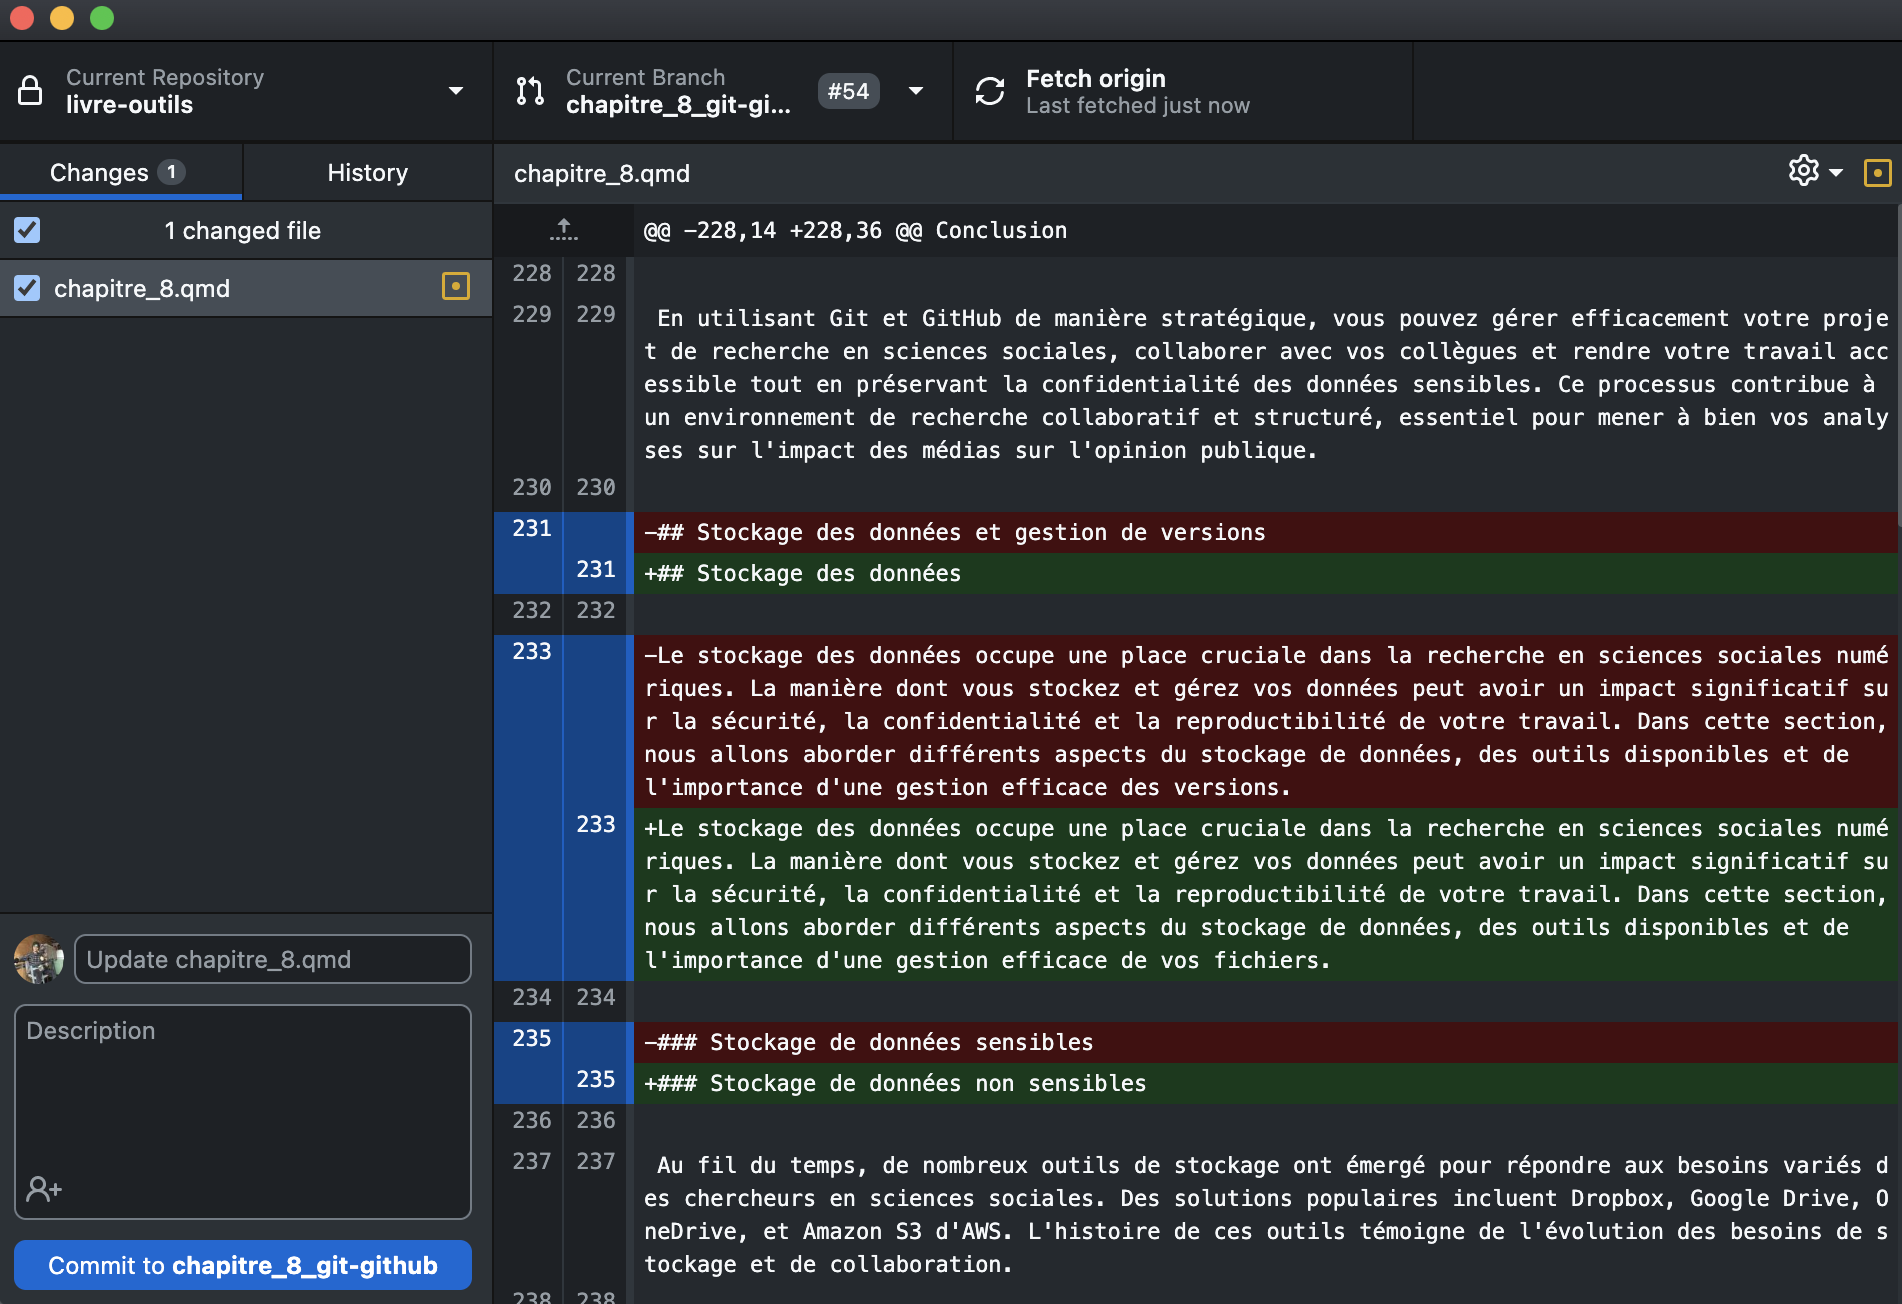
\includegraphics[width=0.8\textwidth,height=\textheight]{images/chapitre8_gitdesktop.png}

}

\caption{\label{fig-github}GitHub Desktop facilite l'utilisation
conjointe de Git et de GitHub.}

\end{figure}%

GitHub Desktop fournit une vue claire de vos répertoires, de vos
modifications, de vos branches et de vos demandes de fusion (\emph{pull
requests}. Il élimine la nécessité de mémoriser les commandes en ligne
de terminal, ce qui peut être un défi pour certains chercheurs.
L'application simplifie également la résolution des conflits lors de la
fusion des branches.

Toutefois, en utilisant GitHub Desktop, il est possible de perdre la
compréhension des commandes Git en ligne de commande, ce qui pourrait
devenir un inconvénient si vous devez travailler dans un environnement
sans interface visuelle. De plus, GitHub Desktop est spécifiquement
conçu pour interagir avec GitHub. Si vous devez travailler avec d'autres
plateformes de gestion de versions, cela pourrait poser des problèmes.

La décision entre l'utilisation du terminal et de GitHub Desktop dépend
de vos préférences et de vos besoins. Pour les chercheurs qui débutent,
GitHub Desktop offre une transition en douceur vers les concepts de
gestion de versions. Cependant, il est important de ne pas se limiter à
une interface visuelle. Comprendre les commandes Git en ligne de
commande reste essentiel pour résoudre des problèmes complexes, gérer
des projets avancés et collaborer avec d'autres chercheurs qui utilisent
des approches basées sur le terminal.

En utilisant Git et GitHub de manière stratégique, vous pouvez gérer
efficacement votre projet de recherche en sciences sociales, collaborer
avec vos collègues et rendre votre travail accessible tout en préservant
la confidentialité des données sensibles. Ce processus contribue à un
environnement de recherche collaboratif et structuré, essentiel pour
mener à bien vos analyses.

Pour utiliser Dropbox efficacement, organisez vos fichiers en
arborescence logique. Créez des dossiers spécifiques pour chaque projet
et partagez-les avec les membres de votre équipe. Pour éviter de pousser
des fichiers sensibles sur GitHub, ajoutez le nom de dossier à exclure
dans un fichier \emph{.gitignore}.

\begin{figure}

\centering{

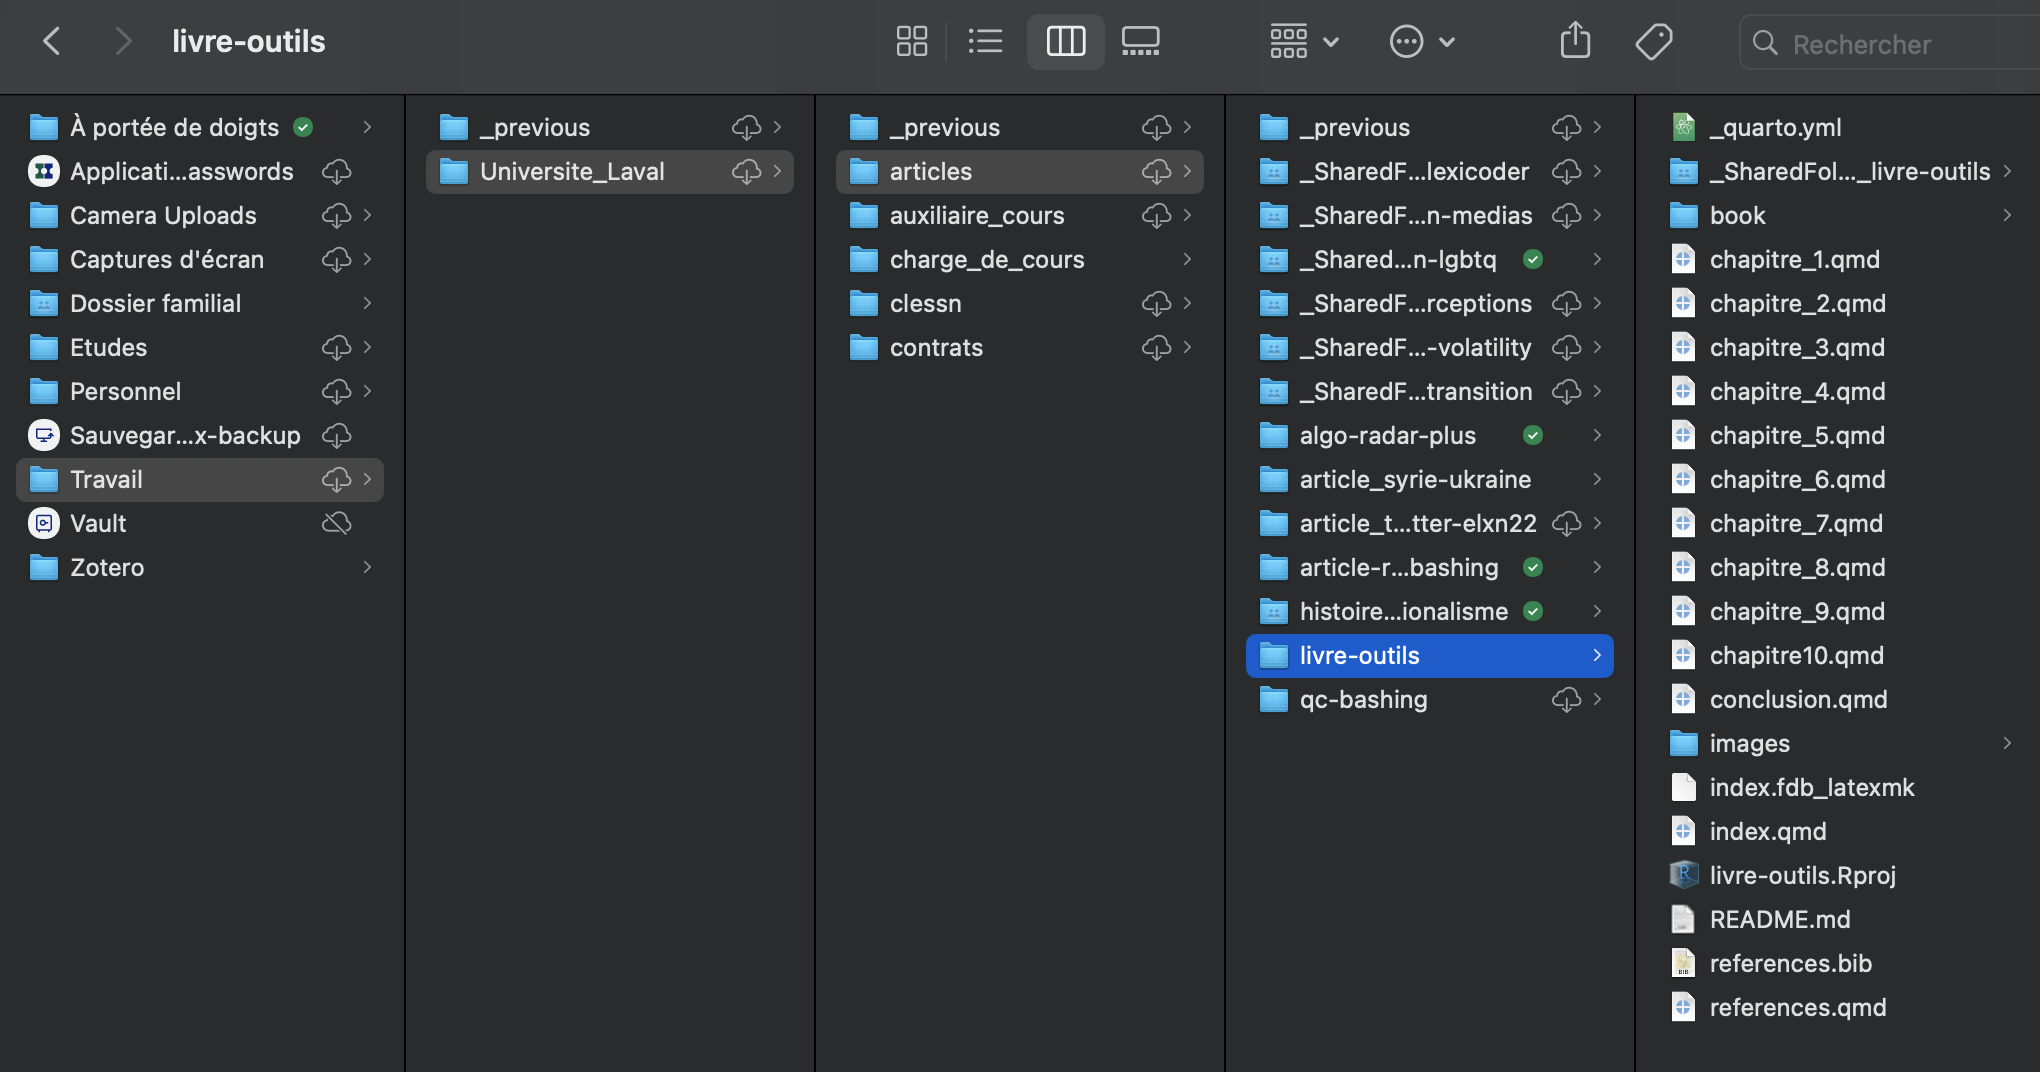
\includegraphics[width=0.8\textwidth,height=\textheight]{images/chapitre8_dropbox.png}

}

\caption{\label{fig-dropbox}Une arborescence claire vers le repository
du livre d'outils en local.}

\end{figure}%

\textless!-- ```

\bookmarksetup{startatroot}

\chapter{Outils de synthèses de la connaissance et de gestion des
références}\label{sec-chap4}

La réalisation d'une synthèse de la connaissance représente la première
marche à franchir avant d'initier tout projet de recherche. C'est en
s'immergeant dans le dialogue établi entre chercheurs qui nous ont
précédés que nous pouvons véritablement saisir l'évolution des idées et
les contours actuels des débats sur un sujet de recherche. Cette
compréhension permet non seulement de cerner les zones de connaissances
encore inexplorées, mais aussi de situer comment inscrire notre propre
recherche dans un domaine circonscrit. Loin d'être une simple collection
de sources choisies aléatoirement, elle doit suivre une démarche
méthodique et réfléchie, intégrant des critères tels que la pertinence,
la crédibilité, la nouveauté sur le sujet, la diversité des
perspectives, la qualité méthodologique, l'impact et la citation des
travaux et leur objectivité.

En choisissant des sources qui répondent à ces exigences, on s'assure
que la revue de littérature offre une perspective complète sur le sujet.
Une grande variété de synthèses de la connaissance existe et chacune
répond à des besoins différents dans le domaine académique, sujet sur
lequel nous reviendrons bientôt.

En dressant un portrait structuré et critique de la littérature
existante, le chercheur établit les fondements de sa démarche
scientifique. Cette étape préliminaire éclaire la formulation de la
question de recherche, en mettant en lumière les interstices où de
nouvelles contributions sont possibles et souhaitables. Ainsi, une revue
de littérature systématique n'est pas simplement un recensement de
connaissances ; c'est une étape cruciale qui façonne le cadre de la
recherche future, garantissant que chaque nouvelle étude contribue aux
connaissances dans un domaine. Cette démarche de synthèse s'accompagne
nécessairement d'une gestion rigoureuse des sources bibliographiques.

La citation des sources quant à elle est une pratique incontournable
dans le monde académique. Elle sert de fondement à la contextualisation
de nos recherches, nous permettant de situer nos travaux au sein d'un
cadre scientifique établi et reconnu. Ce processus de contextualisation
facilite non seulement la compréhension de l'évolution des connaissances
dans un domaine donné, mais contribue également à la création d'une base
de connaissances solide sur laquelle d'autres travaux peuvent être bâtis
(Zaid et al., 2017). La référenciation des travaux antérieurs garantit
la reproductibilité des expériences et des analyses, un pilier central
de la méthodologie scientifique. En fournissant des détails précis sur
les méthodes et résultats, nous ouvrons la voie à la validation et à
l'éventuelle réfutation de nos travaux, renforçant ainsi l'intégrité de
la recherche (Hughes, 2013). De plus, la citation des sources est une
marque de respect envers les contributions des autres chercheurs,
assurant une juste attribution du mérite. Cela reconnaît l'importance de
chaque découverte et idée dans l'avancement de la science, tout en
prévenant le plagiat (Racz \& Marković, 2018). Enfin, une référenciation
minutieuse aide à éviter les biais, en exposant clairement les
fondements sur lesquels se base notre recherche. Cela permet une
évaluation critique des sources et des perspectives, encourageant une
approche plus équilibrée et nuancée dans l'analyse scientifique (Kostoff
\& Cummings, 2013). En résumé, la citation des sources est un acte
fondamental qui englobe et adresse de multiples aspects cruciaux de la
recherche académique : la crédibilité, la contextualisation, la
reproductibilité, la création d'une base de connaissances solide,
l'attribution du mérite et ce, tout en combattant le plagiat et en
minimisant les biais. C'est dans ce contexte que des outils de gestion
des références prennent toute leur importance et que s'inscrit
l'objectif de ce chapitre.

Pour aborder ces enjeux de manière systématique, ce chapitre se
structure autour de quatre axes principaux. Nous commencerons par
explorer les différentes méthodes de synthèse de la connaissance, depuis
la revue narrative jusqu'aux revues systématiques et méta-analyses, en
passant par le snowballing et les revues de portée. Ensuite, nous
examinerons les outils spécialisés pour la synthèse de la connaissance,
avec un focus particulier sur Covidence et ses alternatives comme
Colandr et Rayyan. La troisième section se concentrera sur les outils de
gestion des références, comparant Mendeley, EndNote et Zotero, avant de
détailler pourquoi Zotero constitue un choix optimal pour les
chercheurs. Enfin, nous fournirons un guide pratique d'installation et
d'utilisation de Zotero, incluant la configuration de Better BibTeX pour
une intégration optimale avec LaTeX et Quarto.

\section{Point d'observation: La connaissance et les
références}\label{point-dobservation-la-connaissance-et-les-ruxe9fuxe9rences}

Les synthèses de la connaissance ainsi que la gestion des références ont
longtemps été des processus fastidieux, nécessitant une organisation
rigoureuse des références, des notes de lecture et des articles
accumulés au fil du temps. Avant l'avènement des outils numériques, les
chercheurs dépendaient de méthodes manuelles pour organiser leur
documentation. Les bibliographies étaient construites à la main ou à
l'aide de logiciels de traitement de texte et les articles scientifiques
étaient souvent archivés en version papier dans des classeurs. Cette
gestion physique de la littérature et des références était laborieuse,
sujette aux erreurs et difficile à partager avec d'autres chercheurs ou
collaborateurs.

Le développement des technologies de l'information et la montée en
puissance des bases de données en ligne ont ouvert la voie à l'émergence
d'outils numériques de synthèse de la connaissance et de gestion des
références. À mesure que les ordinateurs devenaient plus accessibles et
que l'informatique évoluait, de nouvelles possibilités se sont offertes
pour organiser et gérer la littérature de manière plus efficace et moins
chronophage. C'est dans ce contexte que les premiers outils numériques
de synthèse de la connaissance et de gestion des références ont vu le
jour.

Ces logiciels de première génération, tels que EndNote (1988) et
Bookends (1988), répondaient à un besoin pressant : faciliter
l'organisation des références ainsi que leur insertion automatique dans
des documents, tout en générant des bibliographies conformes à
différents standards éditoriaux. Cependant, ces outils se sont
rapidement sophistiqués à travers les années. Les logiciels de gestion
de références sont devenus des plateformes centralisées permettant aux
chercheurs de stocker des milliers de citations, de les classer par
mots-clés ou thématiques et de les retrouver facilement. Les
utilisateurs pouvaient aussi importer des références directement depuis
des bases de données en ligne comme PubMed ou JSTOR, automatisant encore
davantage le processus. Aujourd'hui, les outils de synthèse de la
connaissance et de gestion des références, tels que Zotero (2006),
Mendeley (2008) ou Covidence (2014), permettent non seulement de gérer
des bibliographies, mais également de collaborer à plusieurs sur des
revues systématiques, d'annoter des articles, d'organiser des données et
de générer des rapports structurés. Leurs fonctionnalités cloud
facilitent également la synchronisation entre différents appareils et
assurent un accès en tout lieu.

Bien que ce chapitre aborde à la fois les outils de synthèse de la
connaissance et de gestion des références, il est essentiel de préciser
que ces deux types d'outils ont des utilités et fonctionnalités
distinctes. Les outils de synthèse de la connaissance, comme Covidence,
Colandr et Rayyan, sont conçus pour gérer des processus de recherche
plus complexes, tels que les revues systématiques, en facilitant la
sélection, l'évaluation critique et la synthèse des études alors que les
outils de gestion des références, tels que EndNote et Zotero, se
concentrent sur l'organisation, l'annotation et la création de
bibliographies à partir de références.

\begin{figure*}%
\begin{figure}[H]

{\centering 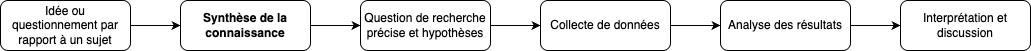
\includegraphics[width=0.8\textwidth,height=\textheight]{images/chapitre4_cycleRecherche.png}

}

\caption{Schéma 1 : Cycle de la recherche scientifique}

\end{figure}%%
\end{figure*}%

Avant d'entrer dans les outils, il convient de glisser quelques mots sur
les méthodes pour lesquelles ces outils sont utiles. Dans le cadre de
l'élaboration d'une recherche scientifique, la phase de synthèse de la
connaissance constitue une étape fondamentale permettant de circonscrire
le champ d'étude, d'identifier les travaux antérieurs pertinents et de
déceler les lacunes dans les connaissances existantes (Schéma 1). Parmi
les différentes approches méthodologiques adoptées pour mener à bien
cette synthèse des connaissances, la revue narrative est généralement la
plus populaire, notamment pour des travaux scolaires ou de courtes
recherches. Des outils comme \emph{Elicit}, \emph{Connected Papers}, ou
\emph{Research Rabbit} sont d'ailleurs très utiles dans ce contexte, car
ils facilitent l'élargissement de la portée de la revue de littérature
en proposant des références supplémentaires ou des publications liées
aux travaux déjà identifiés.

Au-delà de la revue narrative, certaines méthodes comme le
\emph{snowballing} et la revue de portée (\emph{scoping review}) offrent
une approche plus systématique et ciblée. La méthode du snowballing se
distingue par son adaptabilité et sa capacité à englober un large
spectre de travaux pertinents, en particulier dans les phases
préliminaires de la recherche où la question d'étude peut ne pas être
entièrement définie. Le snowballing est une technique de recherche
bibliographique qui se fonde sur la sélection initiale de quelques
publications clés dans le champ d'intérêt. Par la suite, à partir de ces
références clés, le chercheur identifie de manière itérative d'autres
travaux pertinents en examinant les références citées (backward
snowballing) ou les articles citant ces travaux (forward snowballing)
(Nightingale, 2009).

Un deuxième type de synthèse de la connaissance est la revue de portée,
ou scoping review, qui représente une approche systématique et
structurée de revue de la littérature. Elle est principalement utilisée
afin d'explorer des questions de recherche étendues ou complexes. Son
objectif fondamental est de cartographier l'état actuel des
connaissances sur un sujet donné, en identifiant les concepts clés, les
principaux domaines de recherche ainsi que les lacunes existantes dans
un domaine d'étude spécifique (Munn et al., 2018). Cette méthode se
distingue par son champ d'application large et son objectif
exploratoire, permettant ainsi une compréhension holistique des
thématiques étudiées.

Dans le domaine des sciences sociales, les revues systématiques et les
méta-analyses offrent aussi des outils précieux pour synthétiser et
évaluer de manière rigoureuse les preuves issues de multiples études.
Ces approches permettent de dégager des tendances, d'identifier des
consensus ou des divergences dans la littérature et d'éclairer les
débats politiques et sociaux grâce à une base de données empirique
solide. En recensant de manière exhaustive et méthodique la littérature
existante sur un sujet donné, les chercheurs peuvent offrir une synthèse
objective qui reflète l'état actuel des connaissances. La méta-analyse,
souvent intégrée dans le cadre d'une revue systématique, va plus loin en
combinant quantitativement les résultats de différentes études pour
produire une estimation globale de l'effet étudié. Elle offre ainsi une
puissance statistique accrue et une meilleure généralisation des
conclusions, transcendant les limites des études individuelles.

\section{Arpentage et choix éditorial: Les outils de synthèse de la
connaissance}\label{arpentage-et-choix-uxe9ditorial-les-outils-de-synthuxe8se-de-la-connaissance}

Plusieurs outils existent afin de faciliter la vie des chercheurs et
chercheuses qui souhaitent effectuer des synthèses de la connaissance,
chacun répondant à des besoins spécifiques. \emph{Covidence},
\emph{Colandr} et \emph{Rayyan} sont trois outils populaires dans le
monde académique, offrant chacun des fonctions similaires.
\emph{Covidence} est surtout utilisé pour les revues systématiques,
particulièrement dans les domaines de la santé, mais il est également
adaptable aux sciences sociales. Il se distingue par son interface
conviviale, sa gestion collaborative efficace, et son intégration avec
des outils comme EndNote et Zotero. Il est payant, ce qui peut être un
frein pour certains utilisateurs, mais de nombreux établissements
d'enseignement ont une license institutionnelle. Il est généralement
l'outil privilégié par les bibliothèques universitaires. \emph{Colandr},
quant à lui, est un outil gratuit qui se distingue par l'utilisation de
l'intelligence artificielle pour optimiser la sélection des études et
automatiser certaines tâches. Il est particulièrement adapté aux projets
interdisciplinaires, notamment dans les domaines de l'environnement ou
des politiques publiques. Son interface est moins intuitive que celle de
Covidence, mais il reste un excellent choix pour ceux qui cherchent un
outil gratuit et collaboratif. Finalement, \emph{Rayyan} est
probablement l'outil le plus populaire pour les revues systématiques
dans certains domaines, y compris les sciences sociales. Gratuit, il
offre une interface intuitive et utilise des algorithmes pour faciliter
le tri des articles. Toutefois, il propose moins d'options pour
l'extraction des données en comparaison à Covidence.

\subsection{Choix éditorial : Pourquoi Covidence
?}\label{choix-uxe9ditorial-pourquoi-covidence}

L'outil de synthèse de la connaissance Covidence permet une avancée
majeure dans la pratique des revues systématiques, en offrant des
fonctionnalités qui optimisent chaque étape du processus de recherche.
Sa capacité à importer et organiser efficacement les références
provenant de diverses bases de données bibliographiques permet une
gestion structurée des articles à inclure dans une revue. Cet outil
facilite également la collaboration, en permettant à plusieurs
chercheurs de travailler simultanément sur un même projet. En
automatisant les premières phases de sélection des articles, il réduit
la charge de travail manuel et limite les biais potentiels. De plus, ses
moyens d'extraction de données et d'évaluation de la qualité assurent
une analyse rigoureuse et cohérente des résultats. Enfin, son
intégration avec d'autres plateformes de recherche en renforce la
compatibilité et l'efficacité dans le flux de travail académique.

Bien que Covidence soit développé par une organisation à but non
lucratif, il ne répond pas pleinement aux critères du logiciel libre,
car son code source n'est pas accessible pour modification ou
redistribution par la communauté. Cette limitation peut freiner les
utilisateurs souhaitant personnaliser l'outil en fonction de besoins
spécifiques. Néanmoins, Covidence propose un modèle de licence adapté à
un usage académique et non commercial, rendant l'outil accessible à une
large communauté de chercheurs. L'une de ses principales forces réside
dans son intégration des données issues de multiples bases
bibliographiques, ce qui simplifie considérablement le processus de
revue systématique. Covidence est également compatible avec des outils
de gestion des références comme EndNote et Zotero, facilitant
l'importation et l'organisation des références. De nombreuses
institutions universitaires soutiennent l'outil, offrant des licences
institutionnelles pour en élargir l'accès.

En outre, l'interface intuitive de Covidence réduit la courbe
d'apprentissage, guidant les utilisateurs à travers les différentes
phases de la revue systématique de manière structurée et simplifiée par
rapport aux méthodes traditionnelles. Ses fonctionnalités de double
codage, de filtrage et d'extraction de données garantissent une
méthodologie rigoureuse et standardisée, indispensable pour assurer la
qualité des revues systématiques. De plus, Covidence excelle dans la
facilitation de la collaboration entre chercheurs. La plateforme permet
à plusieurs utilisateurs de travailler simultanément sur un même projet,
d'échanger sur l'inclusion ou l'exclusion d'études, et de résoudre
efficacement les divergences, ce qui s'avère particulièrement précieux
pour les projets de grande envergure impliquant des équipes dispersées
géographiquement.

Cependant, l'utilisation de Covidence présente certaines contraintes. Le
coût de l'abonnement peut constituer un frein pour certains chercheurs,
limitant ainsi l'accès à cet outil pourtant utile en recherche. De plus,
bien que Covidence propose des modèles standards pour l'extraction de
données et l'évaluation de la qualité, ces derniers peuvent ne pas
convenir à tous les types d'études, en particulier celles nécessitant
une personnalisation plus poussée. Malgré ces défis, Covidence demeure
un atout précieux pour la réalisation de revues systématiques, bien
qu'il soit essentiel de peser soigneusement ses avantages et
inconvénients en fonction des besoins spécifiques de chaque projet de
recherche.

\begin{table}
\centering
\begin{talltblr}[         %% tabularray outer open
caption={Résumé des principaux outils de gestion de la connaissance},
]                     %% tabularray outer close
{                     %% tabularray inner open
width={0.75\linewidth},
colspec={X[]X[]X[]X[]},
}                     %% tabularray inner close
\toprule
Critères & Covidence & Colandr & Rayyan \\ \midrule %% TinyTableHeader
Accessibilité (Gratuit ou peu dispendieux) & Non (Abonnement requis) & Oui (Gratuit) & Oui (Freemium) \\
Existence d'une communauté d'utilisateurs & Oui & Modérée & Oui \\
Popularité dans le champ & Très populaire dans la revue systématique & Moins connu mais en croissance & Populaire pour la revue systématique \\
Compatibilité avec d'autres outils & Oui (Importation facile de citations) & Oui (supports RIS, BibTeX, etc.) & Oui (Intégration facile avec citation managers) \\
Transparence et réplicabilité & Non (propriétaire) & Oui (Open-source) & Partiellement (propriétaire) \\
Adaptabilité et flexibilité & Oui (mais limité) & Oui (beaucoup de flexibilité) & Oui (partiellement flexible) \\
\bottomrule
\end{talltblr}
\end{table}

\section{Manuel d'instruction: Comment utiliser
Covidence}\label{manuel-dinstruction-comment-utiliser-covidence}

Reconnu pour ses trois phases méthodiques --- « Title and abstract
screening », « Full text review » et « Extraction » --- Covidence
facilite l'importation de données volumineuses depuis des bases de
données bibliographiques et interroge plusieurs bibliothèques. Cela
offre un accès à des milliers d'études pertinentes qui aident les
chercheurs à élaborer un cadre théorique exhaustif. Comme mentionné dans
la section précédente, les méthodes justifiants une utilisation de
Covidence impliquent généralement un double codage, ce qui signifie que
l'évaluation des études est effectuée manuellement par deux codeurs,
permettant ainsi une analyse rigoureuse et détaillée de la littérature
recueillie.

La première phase, le « Title and abstract screening », consiste à
examiner les titres et résumés des articles récupérés. Pour optimiser
cette tâche, il est crucial de définir des critères précis afin
d'évaluer la pertinence des articles relativement au sujet étudié.
Durant cette étape, souvent prolongée en raison du volume conséquent de
la littérature, les chercheurs doivent régulièrement se consulter pour
résoudre les divergences d'opinions et parvenir à un consensus.

Suite à la révision des titres et des résumés, vient le « Full text
review ». Cette deuxième phase implique l'examen complet des textes
sélectionnés lors de l'étape précédente. Les chercheurs doivent alors
voter « oui », « non », ou « peut-être » afin de décider de la
conservation des textes, ce qui peut inclure ou exclure un article ou le
faire progresser vers l'étape suivante. Cette phase, bien qu'elle
concerne moins de documents, reste exigeante et chronophage
principalement en raison des délibérations nécessaires pour arbitrer les
divergences de points de vue.

La phase finale, celle de l'extraction des données, implique la collecte
d'informations pertinentes des études finalement retenues, basée sur un
schéma de codification prédéfini. L'objectif est de parvenir à un
consensus parmi les codeurs. L'extraction dévoile les cadres théoriques,
les méthodologies employées ainsi que les conclusions principales des
recherches sélectionnées.

Une fois les étapes de la revue systématique achevées, la plateforme
Covidence facilite l'exportation des données extraites sous forme de
tableaux, de graphiques et de rapports, destinés à être utilisés dans
des analyses subséquentes ou dans la rédaction d'articles scientifiques.
Bien que Covidence soit largement utilisé et supporté par de nombreuses
universités via des licences, d'autres plateformes comme Colandr et
Rayyan sont également populaires parmi les chercheurs, chacune répondant
à des besoins et des budgets variés.

\section{Arpentage et choix éditorial: Les outils de gestion des
références}\label{arpentage-et-choix-uxe9ditorial-les-outils-de-gestion-des-ruxe9fuxe9rences}

Dans le domaine des outils de gestion des références, Mendeley et
EndNote sont deux solutions populaires utilisées par les étudiants et
les chercheurs à travers le monde. Bien que similaires dans leurs
fonctions principales, ils se distinguent par plusieurs aspects qui
influencent le choix des utilisateurs en fonction de leurs besoins
spécifiques.

Mendeley, développé par Elsevier, est un logiciel gratuit avec des
options payantes pour étendre l'espace de stockage en ligne. Il se
caractérise par son réseau social intégré, permettant aux utilisateurs
de partager leurs références et de collaborer avec d'autres chercheurs.
Mendeley offre également une fonction d'annotation de documents PDF, un
gestionnaire de citations, ainsi qu'une application de bureau et mobile.
Toutefois, Mendeley est parfois critiqué pour sa dépendance vis-à-vis
d'un service centralisé et pour ses politiques de confidentialité, liées
à son appartenance à la compagnie Elsevier.

EndNote, quant à lui, est un logiciel commercial développé par
Clarivate. EndNote se distingue par ses nombreuses fonctionnalités pour
la gestion de grandes bibliothèques de références, une compatibilité
avancée avec les styles de citations et une intégration fluide avec
Microsoft Word. Il est souvent préféré dans les environnements
académiques qui exigent des références complexes ou un large nombre de
sources. Cependant, son coût d'acquisition élevé et l'absence d'une
communauté open source active peuvent être des freins pour certains
utilisateurs, notamment ceux qui privilégient l'accès à des outils
gratuits ou collaboratifs.

\subsection{Choix éditorial : Pourquoi Zotero
?}\label{choix-uxe9ditorial-pourquoi-zotero}

Dans l'écosystème des outils de gestion bibliographique, plusieurs
solutions s'offrent aux chercheurs. Bien que chacune présente ses
propres avantages, comme mentionné précédemment, notre choix s'est porté
sur Zotero pour des raisons à la fois techniques, économiques et
méthodologiques que nous détaillons ci-après. Zotero se distingue des
autres outils de gestion des références par sa gratuité et son
accessibilité en tant que logiciel libre, avec un code ouvert largement
soutenu par une communauté active sur GitHub, qui compte plus de 13 000
contributions. Ce logiciel propose une vaste gamme de fonctionnalités et
permet l'ajout d'extensions pour enrichir son utilisation, ce qui le
rend particulièrement puissant tout en restant facile à utiliser. Zotero
est compatible avec diverses plateformes, notamment Windows, Mac, Linux,
iOS et Android, facilitant ainsi la collaboration entre les membres
d'une équipe de recherche qui utilisent différents systèmes. La
bibliothèque Zotero peut être synchronisée sur plusieurs appareils via
le service cloud payant de Zotero ou en configurant un espace de
stockage cloud personnel. Ce logiciel s'intègre parfaitement dans les
projets de recherche utilisant LaTeX ou Quarto, permettant de générer et
de maintenir à jour automatiquement des fichiers .bib. De plus, Zotero
fonctionne avec des logiciels de traitement de texte tels que
LibreOffice et Microsoft Office, et offre la possibilité de créer des
bibliographies et des citations dans plus de 9 000 styles de citation
différents, répondant ainsi aux divers besoins des chercheurs. En outre,
il permet d'ajouter directement les documents PDF des références et d'y
prendre des notes, ce qui simplifie considérablement la centralisation
de l'information pertinente pour la recherche.

Zotero offre l'avantage significatif de centraliser les sources
bibliographiques et les fichiers associés, simplifiant grandement le
partage de documents au sein des équipes de recherche. Avec Zotero, il
est possible d'ajouter des PDF et de les synchroniser dans des groupes
de travail, ce qui élimine le besoin de recourir à des dossiers partagés
ou d'envoyer des documents par courriel ou via des plateformes de
partage de fichiers. Cette centralisation permet également de réaliser
des recherches par mot-clé à travers l'ensemble des sources d'une
bibliothèque, facilitant la récupération rapide de sources spécifiques.

Cependant, Zotero présente également quelques inconvénients, notamment
sa gestion parfois difficile de très grandes bibliothèques contenant des
milliers de fichiers, ce qui peut nécessiter l'achat d'espace de
stockage supplémentaire. Bien que performant, le logiciel requiert
parfois la saisie manuelle d'informations que le connecteur intégré ne
détecte pas automatiquement, représentant un potentiel défis pour les
utilisateurs. Ces quelques défis soulignent l'importance d'évaluer les
besoins spécifiques en matière de gestion bibliographique avant de
choisir Zotero comme solution.

Dans le chapitre 7, vous apprendrez à connaître et à utiliser le langage
de balisage LaTeX. Un des avantages majeurs de Zotero réside justement
dans sa capacité à s'intégrer parfaitement avec LaTeX : il est souvent
utilisé en combinaison avec BibLaTeX via l'extension Better BibTeX pour
exporter et actualiser automatiquement des bibliographies au format
.bib. BibLaTeX, une extension moderne pour gérer les bibliographies dans
LaTeX et Quarto, s'utilise couramment avec Biber, un outil de traitement
bibliographique avancé compatible avec BibLaTeX. Biber propose des
fonctionnalités telles que le tri poussé, la gestion de multiples
bibliographies et le traitement de divers formats de données
bibliographiques. BibLaTeX, prenant en charge de nombreuses langues, est
idéal pour la rédaction de documents destinés à un public international.
L'exportation de bibliothèques Zotero sous forme de fichiers .bib pour
leur utilisation avec BibLaTeX est simplifiée grâce à Better BibTeX, qui
assure la mise à jour automatique de ces fichiers. Il est recommandé de
maintenir dans votre fichier .bib uniquement les références utilisées,
organisées par ordre alphabétique, afin de faciliter la collaboration et
le partage des ressources.

\begin{table}
\centering
\begin{talltblr}[         %% tabularray outer open
caption={Résumé des principaux outils},
]                     %% tabularray outer close
{                     %% tabularray inner open
width={0.75\linewidth},
colspec={X[]X[]X[]X[]},
}                     %% tabularray inner close
\toprule
Critères & Zotero & Mendeley & Endnote \\ \midrule %% TinyTableHeader
Accessibilité (Gratuit ou peu dispendieux) & Gratuit & Partiellement payant & Payant \\
Existence d'une communauté d'utilisateurs & Environ 7.5m d'utilisateurs & Oui & Oui \\
Popularité dans le champ & Très populaire & Très populaire & Populaire \\
Compatibilité avec d'autres outils & Oui (Intégration facile avec Word, Google Docs, etc.) & Oui (Microsoft Word, LibreOffice) & Oui (Intégration avec Word) \\
Transparence et réplicabilité & Oui (Open-source) & Partiellement (propriétaire) & Non (propriétaire) \\
Adaptabilité et flexibilité & Oui (personnalisable avec plugins) & Oui (moins flexible que Zotero) & Partiellement (moins flexible) \\
\bottomrule
\end{talltblr}
\end{table}

\section{Manuel d'instruction: Comment utiliser
Zotero}\label{manuel-dinstruction-comment-utiliser-zotero}

\subsection{Installation et
Configuration}\label{installation-et-configuration}

L'intégration de Zotero dans le processus de recherche académique permet
une gestion structurée et efficace des références bibliographiques. Pour
tirer pleinement parti des fonctionnalités de cet outil, il est
essentiel de suivre les étapes suivantes pour l'installation, la
configuration, et l'utilisation des principales fonctionnalités de
Zotero. L'installation de Zotero commence par le téléchargement de
l'application Zotero ainsi que de son extension pour navigateur, Zotero
Connector. Cette extension permet de capturer facilement des références
à partir de sources en ligne. Une fois l'installation terminée, il est
recommandé de créer un compte Zotero via le lien d'inscription. Ce
compte facilitera la synchronisation des données entre différents
appareils et permettra le partage de bibliothèques de références avec
des collaborateurs.

\begin{figure}[H]

{\centering 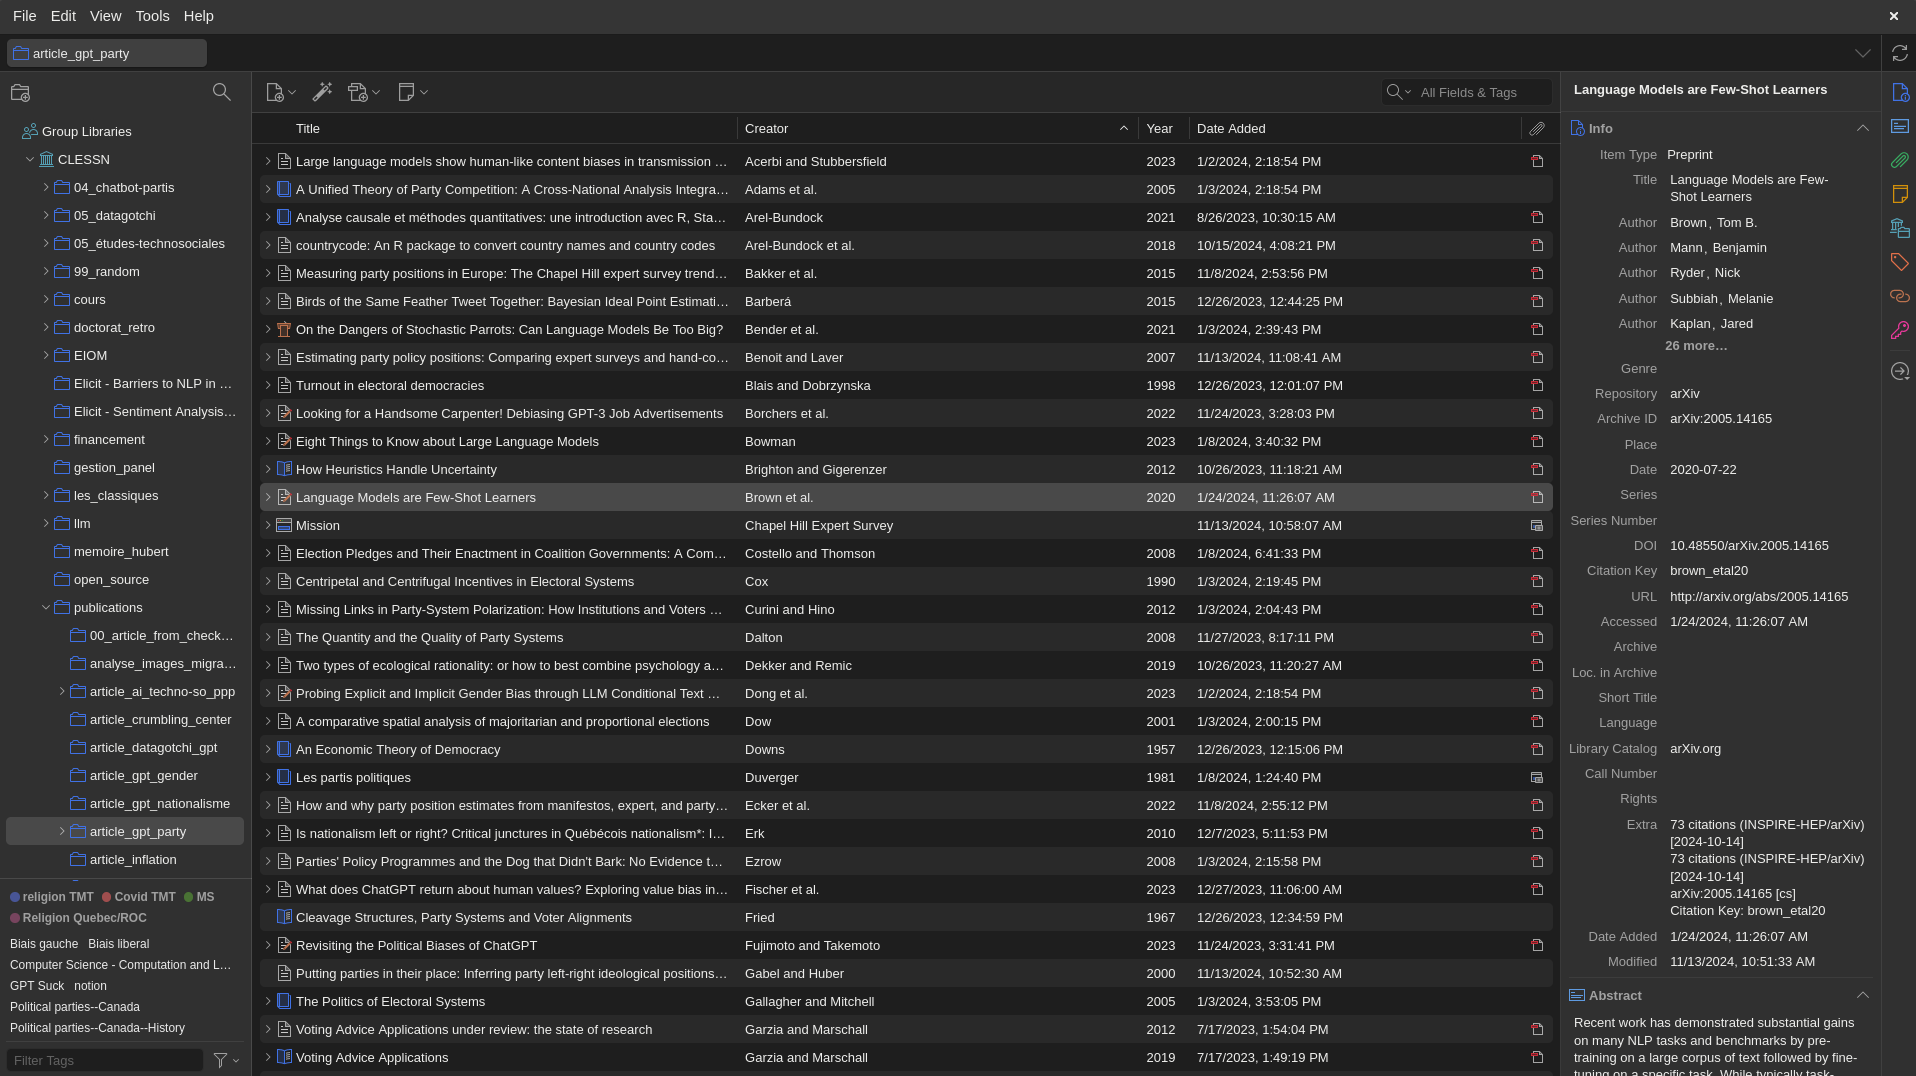
\includegraphics[width=0.8\textwidth,height=\textheight]{images/chapitre4_interface_zotero.png}

}

\caption{Interface principale de Zotero après installation et
configuration initiale}

\end{figure}%

La configuration initiale est essentielle pour exploiter pleinement
Zotero dans un cadre de collaboration. Les chercheurs peuvent créer et
rejoindre des bibliothèques partagées, ce qui permet une gestion
collective des références dans des projets communs.

\subsection{Ajouter des références à
Zotero}\label{ajouter-des-ruxe9fuxe9rences-uxe0-zotero}

Zotero offre plusieurs méthodes pour ajouter des références à une
bibliothèque :

\begin{itemize}
\item
  Glisser-déposer : L'utilisateur peut importer des documents, tels que
  des PDF, directement dans la bibliothèque Zotero. Zotero tentera
  automatiquement de récupérer les métadonnées associées. En cas
  d'échec, l'outil « Baguette magique » permet de saisir manuellement
  les informations requises.
\item
  Utilisation de l'outil Baguette magique : Lorsque des identifiants
  uniques tels que DOI ou ISBN sont disponibles, Zotero extrait
  automatiquement les métadonnées complètes de la référence. Si les
  informations ne sont pas trouvées, l'utilisateur a la possibilité de
  compléter manuellement les champs nécessaires.
\item
  Zotero Connector : Cet outil capture les références directement depuis
  le navigateur, en les classant automatiquement dans les collections de
  la bibliothèque Zotero. Cela permet une gestion instantanée des
  articles scientifiques et autres ressources en ligne.
\end{itemize}

\subsection{Optimisation des citations avec Better
BibTeX}\label{optimisation-des-citations-avec-better-bibtex}

L'installation de l'extension Better BibTeX est cruciale pour les
chercheurs qui utilisent des systèmes de gestion documentaire comme
LaTeX. Cette extension facilite la gestion des citations en générant des
fichiers .bib mis à jour automatiquement.

Pour installer Better BibTeX, dans Zotero, accédez au menu des modules
complémentaires (via le menu \texttt{Outils} sur Windows/Linux ou le
menu \texttt{Zotero} sur macOS, puis \texttt{Modules\ complémentaires}),
puis sélectionnez l'option Installer un module à partir d'un fichier et
choisissez le fichier \texttt{.xpi} préalablement téléchargé. Une fois
l'installation terminée, configurez le module via les préférences de
Zotero (menu \texttt{Édition\ \textgreater{}\ Préférences} sur
Windows/Linux ou \texttt{Zotero\ \textgreater{}\ Préférences} sur macOS)
dans l'onglet Better BibTeX.

Afin d'assurer une cohérence dans les clés de citation utilisées au sein
d'un groupe de travail, Better BibTeX permet de définir un format de clé
de citation uniforme. Le format recommandé est basé sur le nom de
l'auteur et l'année de publication, par exemple :
\texttt{authEtal2.fold.lower.replace(find=".",replace=\_)\ +\ len\ +\ shortyear\ \textbar{}\ veryshorttitle\ +\ shortyear}.
Cette uniformisation garantit une gestion efficace des citations dans
les documents collaboratifs.

\subsection{Génération du fichier
.bib}\label{guxe9nuxe9ration-du-fichier-.bib}

Une fois Better BibTeX configuré, il est possible d'exporter une
collection Zotero au format BibLaTeX. Pour cela, faites un clic droit
sur la collection souhaitée et sélectionnez Exporter la collection.
Choisissez le format \texttt{Better\ BibLaTeX} et cochez l'option
\texttt{{[}x{]}\ Keep\ updated}. Ce fichier \texttt{.bib} sera mis à
jour automatiquement chaque fois que de nouvelles références seront
ajoutées à Zotero. Cette méthode est particulièrement utile pour
synchroniser les références dans des projets partagés via des systèmes
de versionnement comme GitHub.

Il est important de noter que toute modification effectuée dans Zotero
(ajout, suppression de références) sera automatiquement synchronisée
avec les autres membres du groupe. Cela implique qu'une gestion prudente
des références est nécessaire pour éviter toute suppression
accidentelle.

\subsubsection{Utilisation de Zotero lors de la
rédaction}\label{utilisation-de-zotero-lors-de-la-ruxe9daction}

Lors de la rédaction d'articles scientifiques, Zotero peut être intégré
directement dans des éditeurs de texte compatibles avec LaTeX ou
Markdown. L'insertion de références se fait simplement en utilisant la
commande \texttt{@} dans l'éditeur de texte, permettant de sélectionner
rapidement la référence souhaitée à partir de la bibliothèque Zotero.

\section{Conclusion}\label{conclusion-1}

Ce chapitre a exploré l'écosystème des outils de synthèse de la
connaissance et de gestion des références, soulignant leur rôle
fondamental dans la démarche scientifique contemporaine. De la revue
narrative aux méta-analyses, en passant par le snowballing et les revues
de portée, nous avons vu comment différentes approches méthodologiques
répondent à des besoins spécifiques de recherche. Cette diversité
d'approches reflète la richesse et la complexité des questions de
recherche en sciences sociales, nécessitant des outils adaptés à chaque
contexte.

L'évolution technologique a transformé radicalement la pratique de la
recherche bibliographique. Là où les chercheurs dépendaient autrefois de
méthodes manuelles laborieuses, ils disposent aujourd'hui d'outils
sophistiqués comme Covidence pour les revues systématiques et Zotero
pour la gestion des références. Ces plateformes ne se contentent pas de
faciliter le travail individuel ; elles révolutionnent la collaboration
scientifique en permettant le partage instantané de ressources et la
coordination d'équipes dispersées géographiquement.

Notre choix éditorial en faveur de Covidence et Zotero s'appuie sur des
critères précis : accessibilité, transparence, compatibilité et
flexibilité. Zotero, en particulier, illustre parfaitement l'esprit de
la science ouverte grâce à son caractère open-source et sa gratuité,
démocratisant l'accès aux outils de recherche de qualité. Cette
philosophie d'ouverture s'avère importante dans un contexte où la
collaboration interdisciplinaire et internationale devient la norme.
Au-delà des aspects techniques, l'adoption de ces outils représente un
investissement dans la rigueur scientifique. Une gestion méthodique de
la littérature et des références ne constitue pas seulement une exigence
formelle ; elle participe à la construction d'une base de connaissances
fiable et reproductible. Dans un environnement informationnel de plus en
plus dense, ces outils deviennent indispensables pour naviguer dans la
production scientifique et maintenir les standards académiques.

L'apprentissage de ces outils, bien qu'exigeant un investissement
initial en temps, procure des bénéfices qui transcendent les projets
individuels. La maîtrise de Zotero et de Covidence prépare les
chercheurs aux défis futurs de la recherche collaborative et leur permet
de se concentrer sur l'essentiel : la production de connaissances
nouvelles dans leur domaine d'étude.

\bookmarksetup{startatroot}

\chapter{Outils de collecte de données}\label{sec-chap5}

La révolution numérique engendrée par l'émergence des données massives
et de l'intelligence artificielle représente un important défi pour la
communauté académique en sciences sociales (Burrows \& Savage, 2014;
Manovich, 2011). Elle constitue également une opportunité de recherche
enrichissante et innovante permettant une compréhension accrue des
phénomènes sociaux étudiés par la communauté scientifique (Connelly et
al., 2016). Cette meilleure compréhension est permise, entre autres, par
l'accès à une variété inégalée et une quantité massive de données
permettant l'étude des différents objets de recherche (A. D. I. Kramer
et al., 2014; Schroeder, 2014). Si l'accès à ces données numériques
massives représente un défi éthique et théorique, il représente
également un défi technique pour les chercheurs voulant exploiter le
potentiel et les opportunités offertes par les données massives
numériques (Burrows \& Savage, 2014).

Le chapitre qui suit vise à présenter la méthode de l'extraction de
données web, ou \emph{web scraping}, qui permet de récolter des données
provenant de sites internet de manière automatisée. Si le chapitre offre
également un bref survol de différents outils de collectes de données
pouvant être exploités par les scientifiques désirant entreprendre des
recherches en sciences sociales, ce dernier vise surtout à mettre
l'accent sur les opportunités offertes par le numérique. En effet, la
portée de ce chapitre s'étend plus loin que les outils traditionnels de
collecte de données en abordant le potentiel émanant de la programmation
en matière de récolte de données brutes pouvant être analysées par les
chercheurs.ses. Le chapitre débute par une description courte et
non-exhaustive d'outils de collecte de divers types de données
sélectionnés en raison de la portée de leur utilisation ou encore en
raison de leur capacités techniques. Cette section aborde, notamment,
des outils de collecte de données de sondage ou encore des données
textuelles de médias. L'objectif de cette courte section est de
présenter des outils plus traditionnels de collecte de données, certes
efficaces, mais qui comportent un certain nombre de limites. Les
sections suivantes, représentant le coeur de ce chapitre, mettent un
accent particulier sur la méthode de l'extraction de données par le
biais de l'outil \emph{rvest} et les opportunités de recherche qui en
découlent. Il sera question de démontrer comment les capacités de
programmation avec R permettent l'accès à un volume important de données
qui peuvent alimenter de manière significative des projets de recherche.
En somme, ce chapitre offre un tour d'horizon des outils disponibles à
la communauté scientifique tout en présentant les manières d'exploiter
l'extraction web et le package \emph{rvest} et en offrant des exemples
concrets de son utilisation.

\section{\texorpdfstring{\textbf{Point d'observation: les outils
traditionnels de collecte de données numériques en sciences
sociales}}{Point d'observation: les outils traditionnels de collecte de données numériques en sciences sociales}}\label{point-dobservation-les-outils-traditionnels-de-collecte-de-donnuxe9es-numuxe9riques-en-sciences-sociales}

Toute recherche empirique repose sur l'analyse d'un objet de recherche,
et doit donc comprendre une réflexion sur les manières d'observer
l'objet d'étude. Avant l'utilisation de quelconque méthode, il faut un
ensemble de données à analyser sur lesquelles les différentes méthodes
seront appliquées. Le type de données à analyser dépend de l'objectif
analytique de la recherche entreprise, mais surtout, de l'objet de
recherche. Une fois que l'on sait \emph{qu'est} ce qu'on veut étudier,
il faut déterminer \emph{comment} l'étudier, et ultimement, acquérir les
données nécessaires à l'analyse. Les sciences sociales reposent sur
l'analyse des sociétés et des phénomènes qui les caractérisent. Les
objets d'études sont multiples, tout comme les manières de les observer.
Les communautés scientifiques autant qualitatives que quantitatives ont
donc besoin de données qui permettent de tels types d'analyses, et il
existe un immense éventail d'outils permettant la collecte de données
nécessaires à la tenue de recherche en sciences sociales.

\emph{Les données d'entrevues}

L'exemple des entrevues représente bien l'étendue des manières de
récolter des données en sciences sociales. Les entrevues (dirigée,
semi-dirigée ou non-dirigée) sont des méthodes de recherche largement
employées en sciences sociales, et peuvent constituer un outil de
collecte de données qui permet d'aller récolter un savoir pouvant par la
suite être analysé sous forme de texte retranscrit. Il s'agit d'une
méthode particulièrement efficace pour comprendre certains phénonènes
sociaux de manière approfondie et granulaire. Bien que l'objectif de ce
chapitre ne soit pas de présenter les manières de conduire ou analyser
une entrevue en sciences sociales, il demeure pertinent de mentionner
cette méthode afin d'illusrer l'immensité du champ de la collecte de
données. Les prochaines lignes présentent quelques outils de collecte de
données particulièrement prisés en sciences sociales, soit les données
de sondages et les données de médias, et comment l'émergence du
numérique a radicalement transformé le processus d'acquisition de telles
données. Il est important de noter que les données de sondages et les
textes médiatiques se prêtent tout aussi bien aux analyses quantitatives
que qualitatives. L'objectif des prochaines lignes vise donc à présenter
des outils de qui se démarquent par la portée analytique des données
qu'ils permettent de récolter.

\emph{Les données de sondages}

L'opinion publique, une composante fondamentale des sciences sociales,
est traditionnellement étudiée par le biais de données de sondages.
L'émergence des technologies numériques a grandement transformé la
collecte de données de sondages, qui sont désormais conceptualisés et
administrés de manière beaucoup plus efficace. En effet, le numérique
permet donc de créer un questionnaire, de cibler une population et de la
contacter, d'entreposer les données des répondants pour ainsi les
visualiser, le tout à un coût réduit et plus rapidement que s'il avait
été conduit manuellement (Nayak \& KA, 2019). Ainsi, les sondages en
ligne ont une portée internationale, permettent le suivi de la ligne du
temps, offrent des options qui contraignent le répondant à répondre à
certaines questions et permettent d'utiliser des arbres de logique
avancés que les sondages manuels ne permettent pas. Parmi les
plateformes web les plus reconnues de construction et d'administration
de sondage, Qualtrics figure en tête de liste. Cette plateforme est une
des plus reconnues et utilisée à l'international, tant dans le milieu
académique que dans le secteur privé. En plus d'offrir des outils de
collecte de données et de sondages, Qualtrics est utilisé dans le
marketing et dans la gestion de l'expérience client. Il est donc
pertinent de se familiariser avec cet outil, car il offre des
compétences pratiques pour la recherche, mais également pour obtenir des
opportunités de carrière. Qualtrics offre plusieurs services pratiques
pour la collecte de données, avec des options flexibles pour la
programmation et l'administration des sondages. Par exemple, Qualtrics
s'adapte à différents formats en fonction de l'appareil du répondant
(Evans \& Mathur, 2018). Son principal désavantage provient de son coût
d'acquisition, qui est extrêmement dispendieux. La présentation de cet
outil dans le cadre de ce chapitre provient du fait qu'il s'agit de la
principale plateforme de construction de sondage, autant dans le monde
commercial qu'académique. Il devient d'autant plus important de
présenter cet outil en raison du fait que, malgré l'obstacle monétaire,
certaines universités possèdent des licenses permettant l'utilisation de
l'outil par la communauté étudiante. De plus, de nombreus.e.s
professeur.e.s possèdent également des comptes Qualtrics qui permettent
la construction de sondage.

Il convient toutefois de mentionner certaines alternatives à Qualtrics
en raison des obstacles monétaires à son utilisation, tels que Research
Electronic Data Capture (REDCap), Survey Monkey ou encore Google Forms,
qui sont tous des outils permettant d'administrer des sondages.
Toutefois, Qualtrics demeure l'outil le plus utilisé en sciences
sociales (et dans le monde des affaires) en ce qui concerne
l'administration de sondage, ce qui explique la plus grande attention
portée envers cette plateforme. De plus, le chapitre porte
principalement sur la méthode du web scraping. Ainsi, bien qu'il
convienne de présenter des outils plus traditionnels, il se concentre
principalement sur les opportunités offertes par le numérique, ce qui
explique ce survol bref et incomplet des outils de récolte de données de
sondages.

\emph{Les données médiatiques}

La recherche en sciences sociales se penche également sur l'analyse de
contenu médiatique, qui permet une mutltitude de devis de recherche dans
un grand nombre de sous-discipline des sciences sociales. L'émergence du
numérique facilite largement la récolte de données médiatiques tout en
favorisant de nouvelles avenues de recherche pour les chercheurs.euses
en sciences sociales en raison de l'importante quantité de données
accessibles aux chercheurs.euses. À cet effet, l'outil Factiva offre un
accès à l'ensemble des articles d'une panoplie de médias provenant d'une
vaste sélection de pays. Le moteur de recherche est opéré par Dow Jones
et offre également l'accès à des documents d'entreprises. En revanche,
l'accès qu'il offre aux contenus médiatiques est particulièrement
pertinent pour la communauté scientifique en communication et en
sciences sociales. Il offre l'accès à plus de 15 000 sources médiatiques
provenant de 120 pays. Il permet de télécharger une quantité illimitée
de documents RTF, un format de fichier de texte, pouvant contenir
jusqu'à 100 articles chacun. En outre, ils peuvent être sélectionnés
automatiquement en cochant le bouton proposant de sélectionner les 100
articles de la page de résultat. Chaque page de résultat contient 100
articles à la fois. Enfin, Factiva permet également de filtrer les
doublons. Ainsi, Factiva permet d'avoir accès facilement à des données
utiles pour l'analyse textuelle d'articles médiatiques. Comme les textes
deviennent accessibles rapidement et simplement aux chercheurs.euses,
cet outil optimise considérablement l'analyse de contenu par thèmes ou
par ton. Cependant, ce ne sont pas tous les médias qui sont accessibles
sur Factiva. Dans l'optique ou un média recherché n'est pas trouvable
sur cette plateforme, le logiciel Eureka représente une bonne
alternative. Eureka se concentre principalement sur les médias
francophones (autant au Québec qu'en Europe). La structure d'Eureka est
similaire à celle de Factiva.

Ces outils sont très utiles et relativement faciles à utiliser. Il ne
faut toutefois pas tomber dans le piège de se limiter aux outils
traditionnels de recherche. En effet, les récentes transformations
technologiques élargissent considérablement le champ de possibilités
offertes à la communauté scientifique, notamment en raison de la nature
massive des données qui lui est accessible. Non seulement ces données
sont nombreuses, mais elles sont accessibles par le biais de
connaissances de base en programmation. La section suivante aborde un
outil fondamental de la collecte de données en sciences sociales
numériques: les extracteurs webs.

\section{\texorpdfstring{\textbf{Arpentage et choix éditorial:
l'extraction de données web grâce à l'outil
\emph{rvest}}}{Arpentage et choix éditorial: l'extraction de données web grâce à l'outil rvest}}\label{arpentage-et-choix-uxe9ditorial-lextraction-de-donnuxe9es-web-gruxe2ce-uxe0-loutil-rvest}

Les extracteurs de données sont des outils qui ont transformé la récolte
de données en sciences sociales. Les extracteurs de données numériques
sont des infrastructures de code permettant d'extraire des données
brutes d'une source numérique définie. Cette section explique comment
ces extracteurs peuvent être utiles dans un contexte de recherche en
sciences sociales numériques.

L'émergence du numérique représente une opportunité hors pair d'accès à
un volume important de données, qui permettent ainsi une analyse
approfondie des phénomènes politiques contemporains. Toutefois, l'accès
à de telles données peut s'avérer complexe, non-fiable ou encore
coûteux. Par exemple, des données parlementaires peuvent être
accessibles sur les sites internet des parlements et institutions en
questions. L'accès à ces données se voit toutefois complexifié par la
nécessité d'avoir des identifiants ou encore de payer pour les dites
données. De plus, la qualité de ces données n'est pas assurée, en plus
du fait qu'elles peuvent être mal-structurées. Ainsi, l'accès à des
données massives représente un défi considérable pour la communauté
scientifique tentant d'entreprendre des recherches utilisant un volume
important de données.

C'est dans cette optique que les extracteurs de données numériques
peuvent être utiles. Il faut faire ici la distinction entre l'outil,
soit l'extracteur de données, et la méthode, l'extraction web. Plus
précisément, cette dernière est la méthode qui permet l'extraction de
données provenant de sites webs qui seront ensuite converties dans un
format utile aux scientifiques de données. L'extracteur est l'outil qui
permet cette méthode. Il sera question dans les lignes qui suivent de
l'outil \emph{rvest}, un package sur R, qui permet de récolter des
données de site web gratuitement et efficacement.

Il faut toutefois être vigilant quant à la nature des données extraites.
Avant d'extraire quelconque information, il est absolument primordial de
s'assurer que les données soient publiques, faute de quoi l'extraction
serait illégale. Il est donc recommandé de prendre connaissance des
termes et conditions des sites webs étudiés afin de s'assurer de la
légalité de l'extraction de données. Il est également important de
respecter toute norme de droit d'auteurs et de propriété intellectuelles
ou physique des données. De plus, ce n'est pas parce que des données
sont publiques qu'il est nécessairement légal de les extraire et de les
utiliser en recherche. En effet, il ne faut pas faire ressortir dans les
données extraites quelconque information privée qui pourrait permettre
d'identifier des individus (comme des numéros de téléphone, des adresses
courriels, des codes postaux, etc.)

L'utilisation de cet outil est toutefois facilitée par l'existence d'API
(\emph{Application Programming Interface}) sur les plateformes
exploitées. L'API d'un site ou d'une application, souvent fournie par le
site, permet à un tierce partie d'avoir accès à du code expliquant le
fonctionnement de la plateforme étudiée, ce qui en facilite l'extraction
de données. Par exemple, Twitter possédait, avant les changements de
directions récents, un API qui facilitait l'élaboration d'un extracteur.
En contrepartie, Facebook ne possède pas d'API, ce qui rend l'accès à
ses données beaucoup plus complexe. Un API fournit des données
structurées dans un format lisible tel que JSON (JavaScript Object
Notation). En raison de l'automatisation, les API réduisent les chances
d'erreurs dans le processus de scraping, ils ont tendance à maintenir
une interface plus stable et conviviale. C'est un grand changement
comparé aux fichiers HTML, où ces derniers ont des mises en page qui
changent fréquemment de structure.

Un extracteur peut également offrir l'accès à des données médiatiques,
en codant un accès à des fils RSS ou encore aux HTML des médias
extraits. Les fils RSS sont des formats de données qu'il est possible de
recevoir automatiquement lors de mise à jour sur un site particulier.
Par exemple, La Presse change ses Unes plusieurs fois dans une même
journée. En extractant l'accès aux fils RSS, il est possible de recevoir
lesdites mises à jour automatiquement. Ce processus accélère grandement
la collecte de données.

Finalement, les API simplifient le travail de chacun par les mises à
jour et maintenances. Pour être plus précis, les API, étant maintenus
par les fournisseurs de services, sont modifiés au fur et à mesure que
le site évolue. Par exemple, si la structure de X est modifiée, son API
sera également modifié. Cela évite à ceux demandant l'accès d'ajuster
leurs scripts de scraping pour prendre en compte les changements sur le
site.

Il faut cependant être alerte de l'évolution constante de ces outils. En
effet, la présence de données ouvertes et la création croissante d'API
tend à modifier de manière progressive l'outil. Prenons l'exemple de
l'API de X (anciennement Twitter), qui a restreint les accès accordés et
augmentés les coûts pour récupérer les informations sur la plateforme.
Il faut donc rester à l'affût de ces possibles modifications.

En somme, les extracteurs webs, et dans ce cas précis le package rvest,
sont des outils qui facilitent grandement l'acquisition de données
massives. Plutôt que d'avoir à payer pour des données dont la qualité
n'est pas assurée, l'utilisation d'extracteurs permet un accès plus
facile et précis à des données provenant de sites web. L'utilisation de
ces outils peut toutefois s'avérer complexe et nécessitent un certain
nombre de connaissances en lien avec les langages de programmation. Le
chapitre 2 offre un survol du langage fonctionnel R, qui est utilisé par
de nombreux développeurs lors de l'écriture d'extracteurs et qui permet
d'utiliser le package \emph{rvest}. R est également reconnu pour ces
fonctionnalités statistiques qui sont, elles aussi, abordées
ultérieurement dans ce livre. L'utilisation de cet outil permet aux
chercheurs de faire plusieurs coups d'une seule pierre. Non seulement
\emph{rvest} permet de se familiariser avec le langage R, ce qui est un
atout essentiel dans la recherche en sciences sociales numériques, mais
ce même développement permet un accès inégalé à des données massives qui
pourront ensuite être analysées. Ainsi, des connaissances en R sont un
atout fondamental au développement d'extracteurs, et la complexité du
code évoluera dépendamment du site qui sera extrait.

\subsection{Critères de sélection}\label{crituxe8res-de-suxe9lection-1}

L'extracteur \emph{rvest} est un outil accessible, particulièrement
comme il s'agit d'un outil libre de coûts monétaires. En effet, à moins
de circonstances exceptionnelles, l'extraction avec rvest est gratuite.
Le coût serait plutôt dans l'acquisition de connaissances préalables en
code puis dans l'apprentissage de la méthode d'utilisation. Malgré cette
nuance, l'absence de coûts monétaires liés à cet outil favorise son
accessibilité à l'ensemble de la communauté scientifique. Il est par
exemple possible d'étudier l'opinion publique grâce à l'extraction de
publications sur des médias socionumériques, plutôt que de construire et
administrer des sondages coûteux (voir par exemple l'article de Barbera
et al., 2015).

Additionnellement, l'outil jouit d'une grande communauté d'utilisateurs
rendant accessible leurs connaissances, ce qui favorise la diffusion des
savoirs liés à l'utilisation de cet outil. De nombreux forums d'aide
peuvent alors être consultés gratuitement par les chercheurs.euses
voulant se familiariser avec le package, et plus largement, l'extraction
de données web. De nombreux forums sont présents sur le site Stack
Overflow, et certains chapitres d'ouvrages collectifs vulgarisant
l'utilisation de l'outil sont également dispinible gratuitement en ligne
(voir par exemple le chapitre \emph{Web scraping} du livre \emph{R for
Data Science} d'Hadley Wickham, 2022, qui présente comment utiliser
l'outil \emph{rvest}). Bien que des outils comme Qualtrics et Factiva
aient également un grand nombre d'utilsateurs.ices, ces outils ne se
démarquent pas par la transparence et le partage de leur communauté
utilisatrice.

Les extracteurs sont des outils de recherche très en vogue dans la
communauté des sciences sociales. La possibilité d'obtenir une quantité
importante de données de manière efficace et gratuite représente une
opportunité depuis largement exploitée par les chercheurs en sciences
sociales, en témoigne l'émergence de cours dédiés à l'utilisation
d'outils permettant l'extraction web dans de nombreuses écoles
méthodologiques de renom (telles qu'ICPSR ou ECPR).

Cette méthode, avec le logiciel R, via l'outil \emph{rvest} permet de
récolter des données qui pourront ensuite être traitées et exploiter
avec R, ce qui favorise donc la compatibilité de l'outil. De plus, les
données extraites peuvent être exportées dans de nombreux formats tels
que des fichiers .csv, .RDS, .xlsx, et plus encore.

Tel qu'explicité précédemment, la présence d'une grande communauté
d'utilisateurs de l'outil favorise la transparence et la réplicabilité
des différents résultats produits lors de l'utilisation d'extracteurs.

\section{Manuel d'instruction: extraire des données avec
R}\label{manuel-dinstruction-extraire-des-donnuxe9es-avec-r}

La section suivante présente la méthode d'utilisation de l'outil
\emph{rvest}. Elle démontre comment l'outil permet d'extraire des
données du web, une méthode très en vogue en science sociales.

\subsection{L'importance de comprendre la structure du code
HTML}\label{limportance-de-comprendre-la-structure-du-code-html}

Afin d'être à l'aise avec les extracteurs web, et dans notre cas précis
le package \emph{rvest}, il peut être un atout de se familiariser avec
la structure de base du langage HTML, dont l'acronyme signifie
``Hypertext Markup Language''. Il s'agit d'un langage de code qui permet
la description du contenu de la page web. La structure du code HTML est
hiérarchique, ce qui signifie que le code est divisé en différentes
sections qui occupent différents rôles. Ces sections sont délimitées par
des ``tags'', qui définissent le début ou la fin d'une section du site.
Ce sont ces différentes sections qui seront accessibles pour
l'extraction, et le code HTML permet de comprendre ce qui se situe dans
ces sections. La Figure 5.3 représente un exemple de base de code HTML.

\begin{figure}[H]

{\centering 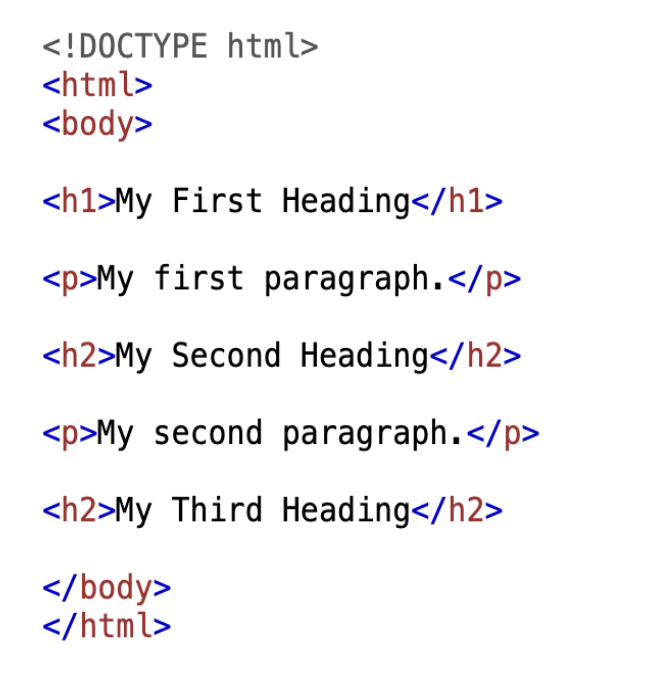
\includegraphics[width=0.8\textwidth,height=\textheight]{images/chapitre5_html_input.png}

}

\caption{Exemple de code HTML}

\end{figure}%

Dans l'exemple ci-haut, le tag \textless h1 représente le titre du HTML.
Le signe \textless p permet de débuter le paragraphe de texte suivant le
titre, et cette section devra être terminée par le sigle p\textgreater.
Les sections \textless p\textgreater{} délimitent les paragraphes écrits
dans chacunes des sections. Les sigles \textless h2\textgreater{}
produisent une sous-section et un sous titre, qui pourra être
complémenté d'un paragraphe écrit. La Figure 5.4 démontre le texte
produit par le code HTML.

\begin{figure}[H]

{\centering 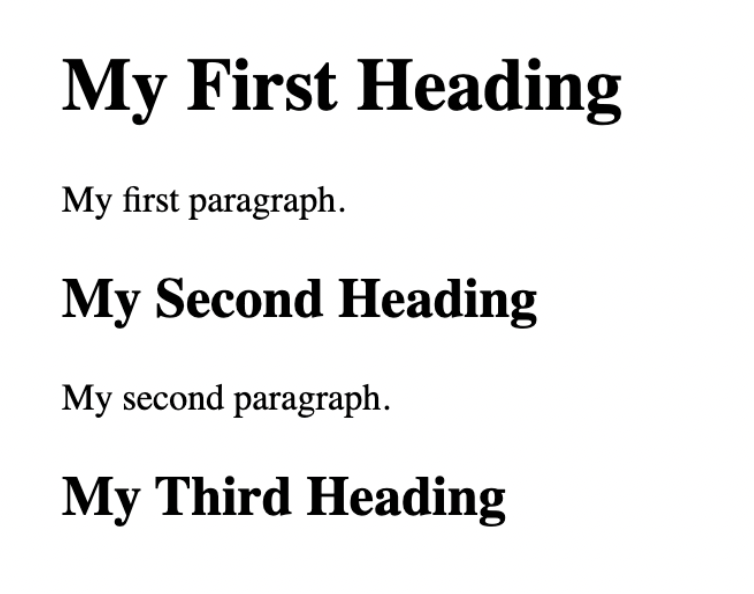
\includegraphics[width=0.8\textwidth,height=\textheight]{images/chapitre5_html_output.png}

}

\caption{Exemple du résultat de code HTML}

\end{figure}%

La structure de base du langage HTML est somme toute simple et intuitive
et tous les sites web sur internet sont fondés sur du code HTML.
N'importe qui étant intéressé à extraire des données de sites webs et
tirer profit de la simplicité et l'accessibilité des données qui peuvent
en émerger devraient donc se familiariser avec ce langage. De nombreuses
sources en ligne sont disponibles afin d'apprendre sur le fonctionnement
du code HTML. Il est donc fortement encourager d'explorer plus en
profondeur les structures du code HTML afin d'obtenir une compréhension
accrue du fonctionnement des sites webs dont on souhaite l'extraction.
Comme le code HTML de chaque site est accessible grâce à l'URL, les
données présentes sur des sites webs sont facilement accessible à la
communauté scientifique.

\subsection{\texorpdfstring{\textbf{Le package rvest: son fonctionnement
et ses
possibilités}}{Le package rvest: son fonctionnement et ses possibilités}}\label{le-package-rvest-son-fonctionnement-et-ses-possibilituxe9s}

Cet ouvrage recommande l'utilisation du paquetage *rvest* afin de
récolter des données sur des pages web, qu'elles aient ou non un API.
Rvest est construit autour des paquetages ``xml2'' et ``httr'' afin de
faciliter la manipulation du HTML et XML. Rvest est principalement conçu
pour scraper une seule page web alors que pour scraper de multiples
pages, d'autres paquetages sont recommandés, notamment ``polite''. Ce
chapitre ne rentre pas dans les détails et ne se concentrera que sur
Rvest.

\subsubsection{\texorpdfstring{\textbf{Fonctions de base du paquetage
rvest utilisant pour exemple le site de
LEGISinfo}}{Fonctions de base du paquetage rvest utilisant pour exemple le site de LEGISinfo}}\label{fonctions-de-base-du-paquetage-rvest-utilisant-pour-exemple-le-site-de-legisinfo}

La première étape est l'installation et le chargement des paquetages
``tidyverse'' et ``rvest'' sur sa console Rstudio. Il est important de
les charger séparément car RVEST ne fait pas partie des paquetages de
base du TIDYVERSE. Nous installerons ce dernier car il amène des
fonctions pratiques au scraping

\begin{Shaded}
\begin{Highlighting}[]
\ExtensionTok{install.packages}\ErrorTok{(}\StringTok{"rvest"}\KeywordTok{)}

\ExtensionTok{install.packages}\ErrorTok{(}\StringTok{"tidyverse"}\KeywordTok{)}

\ExtensionTok{library}\ErrorTok{(}\ExtensionTok{rvest}\KeywordTok{)}

\ExtensionTok{library}\ErrorTok{(}\ExtensionTok{tidyverse}\KeywordTok{)}
\end{Highlighting}
\end{Shaded}

Pour débuter l'extraction des données, il suffit de copier l'URL de la
page web à scraper et la coller dans l'appel de la fonction
read\_html(). Il est important de stocker l'URL dans l'objet
``html\_LEGISinfo.

\begin{Shaded}
\begin{Highlighting}[]
\ExtensionTok{html\_LEGISinfo} \OperatorTok{\textless{}}\NormalTok{{-} read\_html}\ErrorTok{(}\StringTok{"https://www.parl.ca/legisinfo/en/bills"}\KeywordTok{)}

\ExtensionTok{html\_LEGISinfo}
\end{Highlighting}
\end{Shaded}

Lors de l'exécution des lignes de code ci-hautes, la console retournera
les éléments suivants:

\begin{Shaded}
\begin{Highlighting}[]
\ExtensionTok{\{html\_document\}}
\OperatorTok{\textless{}}\NormalTok{html }\VariableTok{lang}\OperatorTok{=}\StringTok{"en"} \ExtensionTok{xml:lang=}\StringTok{"en"}\NormalTok{ xmlns=}\StringTok{"http://www.w3.org/1999/xhtml"}\OperatorTok{\textgreater{}}
\ExtensionTok{[1]} \OperatorTok{\textless{}}\NormalTok{head}\OperatorTok{\textgreater{}}\DataTypeTok{\textbackslash{}n}\OperatorTok{\textless{}}\NormalTok{meta http{-}equiv=}\StringTok{"Content{-}Type"} 
\VariableTok{content}\OperatorTok{=}\StringTok{"text/html; charset=UTF{-}8"}\OperatorTok{\textgreater{}}\DataTypeTok{\textbackslash{}n}\OperatorTok{\textless{}}\NormalTok{meta }
\ExtensionTok{...}
\ExtensionTok{[2]} \OperatorTok{\textless{}}\NormalTok{body class=}\StringTok{"body{-}wrapper ce{-}parl vh{-}100"}\OperatorTok{\textgreater{}}\DataTypeTok{\textbackslash{}r\textbackslash{}n}    
\OperatorTok{\textless{}}\NormalTok{header }\VariableTok{class}\OperatorTok{=}\StringTok{"d{-}print{-}none"}\OperatorTok{\textgreater{}\textless{}}\NormalTok{!{-}{-} }\ExtensionTok{...}
\end{Highlighting}
\end{Shaded}

Une fois que les éléments que l'on souhaite extraire sont déterminés, il
faut les trouver dans le document HTML. Pour ce faire, il faut se
référer au style CSS (cascading style sheets), langage définissant la
forme visuelle d'un document HTML. Les éléments HTML sont identifiés
avec des ``sélecteurs CSS'', ayant pour but de les regrouper pour
faciliter leur extraction. Pour les bases du scraping, il n'est pas
primordial de comprendre les détails des sélecteurs CSS. Seule la
compréhension de la structure d'un document HTML est nécessaire afin
d'en faire l'extraction d'éléments. L'important est d'être en mesure
d'identifier les sélecteurs CSS liés aux éléments souhaités, sans avoir
à comprendre le sélecteur en question.

D'abord, html\_elements doit être utilisé en premier pour trouver toutes
les observations souhaitées, car cette fonction retourne une liste de
tous les noeuds qui matchent avec l'appel de fonction. Le nombre
d'observations est indiqué par xml\_nodeset(). Comme html\_element
retourne seulement le premier élément qui match, il faut l'utiliser en
deuxième, après html\_elements. Cette seconde fonction à pour but de
trouver les éléments qui deviendront les variables à extraire. Pour
l'exemple de LEGISinfo, nous commencerons par extraire tous les éléments
\textbackslash\textless a\textbackslash\textgreater. Comme
html\_elements retourne une liste, nous voulons commencer avec cette
fonction.

\begin{Shaded}
\begin{Highlighting}[]
\ExtensionTok{html\_LEGISinfo} \KeywordTok{|}\OperatorTok{\textgreater{}}\NormalTok{ html\_elements}\KeywordTok{(}\StringTok{"a"}\KeywordTok{)}
\end{Highlighting}
\end{Shaded}

Qui retourne les éléments suivants:

\begin{Shaded}
\begin{Highlighting}[]
\ExtensionTok{\{xml\_nodeset} \ErrorTok{(}\ExtensionTok{180}\KeywordTok{)}\ErrorTok{\}}
 \ExtensionTok{[1]} \OperatorTok{\textless{}}\NormalTok{a href=}\StringTok{"\#StartOfContent"}\NormalTok{ class=}\StringTok{"ce{-}parl{-}skipnav sr{-}only }
\StringTok{ sr{-}only{-}focusable"}\OperatorTok{\textgreater{}}\NormalTok{Skip to m ...}
 \ExtensionTok{[2]} \OperatorTok{\textless{}}\NormalTok{a href=}\StringTok{"//www.parl.ca"}\NormalTok{ class=}\StringTok{"ce{-}parl{-}btn float{-}left text{-}nowrap"}\OperatorTok{\textgreater{}}
 \ExtensionTok{Parliament}\NormalTok{ of Cana ...}
 \ExtensionTok{[3]} \OperatorTok{\textless{}}\NormalTok{a href=}\StringTok{"https://visit.parl.ca/index{-}e.html"}\NormalTok{ rel=}\StringTok{"external"}\OperatorTok{\textgreater{}}\DataTypeTok{\textbackslash{}n\textbackslash{}t\textbackslash{}t}\NormalTok{                    ...}
\end{Highlighting}
\end{Shaded}

\begin{Shaded}
\begin{Highlighting}[]
\ExtensionTok{html\_LEGISinfo} \KeywordTok{|}\OperatorTok{\textgreater{}}\NormalTok{ html\_elements}\KeywordTok{(}\StringTok{"a"}\KeywordTok{)}
\end{Highlighting}
\end{Shaded}

Qui retourne les éléments suivants:

\begin{Shaded}
\begin{Highlighting}[]
\ExtensionTok{\{xml\_nodeset} \ErrorTok{(}\ExtensionTok{180}\KeywordTok{)}\ErrorTok{\}}
 \ExtensionTok{[1]} \OperatorTok{\textless{}}\NormalTok{a href=}\StringTok{"\#StartOfContent"}\NormalTok{ class=}\StringTok{"ce{-}parl{-}skipnav sr{-}only sr{-}only{-}}
\StringTok{ focusable"}\OperatorTok{\textgreater{}}\NormalTok{Skip to m ...}
 \ExtensionTok{[2]} \OperatorTok{\textless{}}\NormalTok{a href=}\StringTok{"//www.parl.ca"}\NormalTok{ class=}\StringTok{"ce{-}parl{-}btn float{-}left text{-}nowrap"}\OperatorTok{\textgreater{}}
 \ExtensionTok{Parliament}\NormalTok{ of Cana ...}
 \ExtensionTok{[3]} \OperatorTok{\textless{}}\NormalTok{a href=}\StringTok{"https://visit.parl.ca/index{-}e.html"}\NormalTok{ rel=}\StringTok{"external"}\OperatorTok{\textgreater{}}\DataTypeTok{\textbackslash{}n\textbackslash{}t\textbackslash{}t}\NormalTok{                    ...}
\end{Highlighting}
\end{Shaded}

\begin{Shaded}
\begin{Highlighting}[]
\ExtensionTok{html\_LEGISinfo} \KeywordTok{|}\OperatorTok{\textgreater{}}\NormalTok{ html\_elements}\KeywordTok{(}\StringTok{"a"}\KeywordTok{)}
\end{Highlighting}
\end{Shaded}

\begin{Shaded}
\begin{Highlighting}[]
\ExtensionTok{\{html\_node\}}
\OperatorTok{\textless{}}\NormalTok{a }\VariableTok{href}\OperatorTok{=}\StringTok{"\#StartOfContent"} \VariableTok{class}\OperatorTok{=}\StringTok{"ce{-}parl{-}skipnav sr{-}only sr{-}only{-}focusable"}\OperatorTok{\textgreater{}}
\end{Highlighting}
\end{Shaded}

Suite à l'inspection des éléments , ceux qui nous intéressent sont ceux
de classe ``bill-tile-container''. Il suffit d'ajouter un point ``.''
avant la classe souhaitée lors de l'appel de la fonction afin de
rechercher les éléments en fonction de leur classe. Les classes HTML
servent à catégoriser les éléments HTML selon un style prédéterminé.
Pour l'exemple de LEGISinfo, nous obtenons une liste d'éléments de
classe bill-tile-container que nous allons stocker dans l'objet
BillTile\_LEGISinfo. Tous les éléments de cette classe auront donc tous
une structure ou des comportements similaires entre eux.

\begin{Shaded}
\begin{Highlighting}[]
\ExtensionTok{BillTile\_LEGISinfo} \OperatorTok{\textless{}}\NormalTok{{-} html\_LEGISinfo }\KeywordTok{|}\OperatorTok{\textgreater{}}\NormalTok{ html\_elements}\KeywordTok{(}\StringTok{".bill{-}tile{-}container"}\KeywordTok{)}
\end{Highlighting}
\end{Shaded}

L'exécution du bloc de code ci-haut produit le résultat suivant dans la
console

\begin{Shaded}
\begin{Highlighting}[]
\ExtensionTok{\{xml\_nodeset} \ErrorTok{(}\ExtensionTok{60}\KeywordTok{)}\ErrorTok{\}}
 \ExtensionTok{[1]} \OperatorTok{\textless{}}\NormalTok{a class=}\StringTok{"bill{-}tile{-}container senate"}\NormalTok{ href=}\StringTok{"/legisinfo/en/bill/44{-}1/s{-}1"}\OperatorTok{\textgreater{}}
 \ExtensionTok{\textbackslash{}r\textbackslash{}n\textbackslash{}r\textbackslash{}n}\NormalTok{     ...}
 \ExtensionTok{[2]} \OperatorTok{\textless{}}\NormalTok{a class=}\StringTok{"bill{-}tile{-}container senate"}\NormalTok{ href=}\StringTok{"/legisinfo/en/bill/44{-}1/s{-}2"}\OperatorTok{\textgreater{}}
 \ExtensionTok{\textbackslash{}r\textbackslash{}n\textbackslash{}r\textbackslash{}n}\NormalTok{     ...}
 \ExtensionTok{[3]} \OperatorTok{\textless{}}\NormalTok{a class=}\StringTok{"bill{-}tile{-}container senate"}\NormalTok{ href=}\StringTok{"/legisinfo/en/bill/44{-}1/s{-}3"}\OperatorTok{\textgreater{}}
 \ExtensionTok{\textbackslash{}r\textbackslash{}n\textbackslash{}r\textbackslash{}n}\NormalTok{     ...}
\end{Highlighting}
\end{Shaded}

À partir de la liste d'éléments de classe bill-tile-container, nous
appelons la fonction html\_element, qui lorsque appliqué à une liste
permet d'extraire la première correspondance de tous les éléments de
cette liste au lieu de seulement retourner le premier nœud correspondant
du document HTML. Nous cherchons à extraire ici les éléments de classe
parliament-session par le biais de la ligne de code suivante:

\begin{Shaded}
\begin{Highlighting}[]
\ExtensionTok{BillTile\_LEGISinfo} \KeywordTok{|}\OperatorTok{\textgreater{}}\NormalTok{ html\_element}\KeywordTok{(}\StringTok{".parliament{-}session"}\KeywordTok{)} 
\end{Highlighting}
\end{Shaded}

Ce qui produit le résultat suivant dans la console:

\begin{Shaded}
\begin{Highlighting}[]
\ExtensionTok{\{xml\_nodeset} \ErrorTok{(}\ExtensionTok{60}\KeywordTok{)}\ErrorTok{\}}
 \ExtensionTok{[1]} \OperatorTok{\textless{}}\NormalTok{div class=}\StringTok{"parliament{-}session"}\OperatorTok{\textgreater{}}\DataTypeTok{\textbackslash{}n}\OperatorTok{\textless{}}\NormalTok{span class=}\StringTok{"parl{-}session{-}number"}\OperatorTok{\textgreater{}}
 \ExtensionTok{44th}\OperatorTok{\textless{}}\NormalTok{/span}\OperatorTok{\textgreater{}}\NormalTok{ Parlia ...}
 \ExtensionTok{[2]} \OperatorTok{\textless{}}\NormalTok{div class=}\StringTok{"parliament{-}session"}\OperatorTok{\textgreater{}}\DataTypeTok{\textbackslash{}n}\OperatorTok{\textless{}}\NormalTok{span class=}\StringTok{"parl{-}session{-}number"}\OperatorTok{\textgreater{}}
 \ExtensionTok{44th}\OperatorTok{\textless{}}\NormalTok{/span}\OperatorTok{\textgreater{}}\NormalTok{ Parlia ...}
 \ExtensionTok{[3]} \OperatorTok{\textless{}}\NormalTok{div class=}\StringTok{"parliament{-}session"}\OperatorTok{\textgreater{}}\DataTypeTok{\textbackslash{}n}\OperatorTok{\textless{}}\NormalTok{span class=}\StringTok{"parl{-}session{-}number"}\OperatorTok{\textgreater{}}
 \ExtensionTok{44th}\OperatorTok{\textless{}}\NormalTok{/span}\OperatorTok{\textgreater{}}\NormalTok{ Parlia ...}
\end{Highlighting}
\end{Shaded}

Bien que moins utile pour la mise en situation actuelle, il est
également possible d'extraire les éléments en fonction de leur ``id
attribute''. Pour ce faire, il faut mettre un hashtag (\#) avant
l'élément à extraire lors de l'appel de la fonction. Le id attribute
retourne toujours un seul élément car ils sont uniques à chaque document
HTML. Voici la ligne de code et le résultat produit par une telle
opération

\begin{Shaded}
\begin{Highlighting}[]
\ExtensionTok{html\_LEGISinfo} \KeywordTok{|}\OperatorTok{\textgreater{}}\NormalTok{ html\_elements}\KeywordTok{(}\StringTok{"\#StartOfContent"}\KeywordTok{)}
\end{Highlighting}
\end{Shaded}

\begin{Shaded}
\begin{Highlighting}[]
\ExtensionTok{\{xml\_nodeset} \ErrorTok{(}\ExtensionTok{1}\KeywordTok{)}\ErrorTok{\}}
\ExtensionTok{[1]} \OperatorTok{\textless{}}\NormalTok{a id=}\StringTok{"StartOfContent"}\NormalTok{ tabindex=}\StringTok{"{-}1"}\OperatorTok{\textgreater{}\textless{}}\NormalTok{/a}\OperatorTok{\textgreater{}}
\end{Highlighting}
\end{Shaded}

Nous avons créé précédemment l'objet BillTile\_LEGISinfo pour ensuite y
extraire les éléments de classe parliament-session. Nous appelons cette
étape l'imbrication des sélections. Lorsque la fonction html\_element
est appliquée à un vecteur de liste html\_elements, la console retourne
le premier nœud correspondant de chaque élément de la liste. Il est
important d'utiliser html\_element à cette étape car il retourne un NA
même lorsqu'il n'y a pas d'éléments correspondants, alors que
html\_elements ne retournera pas la valeur manquante. Dans l'exemple de
LEGISinfo, c'est exactement ce que l'on a voulu faire pour obtenir les
éléments de classe parliament-session. Nous sommes maintenant arrivés à
l'étape d'extraire les données souhaitées. C'est assez simple, il ne
suffit que d'appliquer la fonction html\_text2 sur l'appel de
html\_element sur l'objet à moissonner, dans ce cas ci
BillTile\_LEGISinfo. Il est important de prendre en compte que nous
connaissons ici les éléments à extraire, car le script du document a été
scruté préalablement grâce à la fonction ``inspect'' de Google Chrome
ainsi que les diverses fonctions du package rvest. Afin d'extraire les
autres informations souhaitées, nous allons également créer deux autres
objets qui seront à leur tour moissonnés. Voici les différentes
opérations et leurs résultats dans la console:

Code

\begin{Shaded}
\begin{Highlighting}[]
\ExtensionTok{BillTile\_LEGISinfo} \KeywordTok{|}\OperatorTok{\textgreater{}}\NormalTok{ html\_element}\KeywordTok{(}\StringTok{"h4"}\KeywordTok{)} \KeywordTok{|}\OperatorTok{\textgreater{}}\NormalTok{ html\_text2}\KeywordTok{()}
\end{Highlighting}
\end{Shaded}

Console

\begin{Shaded}
\begin{Highlighting}[]
\ExtensionTok{[1]} \StringTok{"S{-}1"}   \StringTok{"S{-}2"}   \StringTok{"S{-}3"}   \StringTok{"S{-}4"}   \StringTok{"S{-}5"}\NormalTok{...}
\end{Highlighting}
\end{Shaded}

Code

\begin{Shaded}
\begin{Highlighting}[]
\ExtensionTok{BillTile\_LEGISinfo} \KeywordTok{|}\OperatorTok{\textgreater{}}\NormalTok{ html\_element}\KeywordTok{(}\StringTok{".parliament{-}session"}\KeywordTok{)} \KeywordTok{|}\OperatorTok{\textgreater{}}\NormalTok{ html\_text2}\KeywordTok{()}\BuiltInTok{.}
\end{Highlighting}
\end{Shaded}

Console

\begin{Shaded}
\begin{Highlighting}[]
\ExtensionTok{[1]} \StringTok{"44th Parliament, 1st session"} \StringTok{"44th Parliament, 1st session"}\NormalTok{...}
\end{Highlighting}
\end{Shaded}

Code

\begin{Shaded}
\begin{Highlighting}[]
\ExtensionTok{BillTile\_LEGISinfo} \KeywordTok{|}\OperatorTok{\textgreater{}}\NormalTok{ html\_element}\KeywordTok{(}\StringTok{"h5"}\KeywordTok{)} \KeywordTok{|}\OperatorTok{\textgreater{}}\NormalTok{ html\_text2}\KeywordTok{()}
\end{Highlighting}
\end{Shaded}

Console

\begin{Shaded}
\begin{Highlighting}[]
\ExtensionTok{[1]} \StringTok{"An Act relating to railways"}                                                                                                                                                                                                                                                                                  
 \ExtensionTok{[2]} \StringTok{"An Act to amend the Parliament of Canada Act and to make }
\StringTok{ consequential and related amendments to other Acts"}                                                                                                                                                                                                  
 \ExtensionTok{[3]} \StringTok{"An Act to amend the Judges Act"}   
\ExtensionTok{...}
\end{Highlighting}
\end{Shaded}

Code

\begin{Shaded}
\begin{Highlighting}[]
\ExtensionTok{BillBS\_LEGISinfo} \OperatorTok{\textless{}}\NormalTok{{-} html\_LEGISinfo }\KeywordTok{|}\OperatorTok{\textgreater{}}\NormalTok{ html\_elements}\KeywordTok{(}\StringTok{".bottom{-}section"}\KeywordTok{)}
\ExtensionTok{BillBS\_LEGISinfo} \KeywordTok{|}\OperatorTok{\textgreater{}}\NormalTok{ html\_element}\KeywordTok{(}\StringTok{"dd"}\KeywordTok{)} \KeywordTok{|}\OperatorTok{\textgreater{}}\NormalTok{ html\_text2}\KeywordTok{()}
\end{Highlighting}
\end{Shaded}

Console

\begin{Shaded}
\begin{Highlighting}[]
\ExtensionTok{[1]} \StringTok{"Introduced as pro forma bill"}                                 
\StringTok{"Senate bill awaiting first reading in the House of Commons"}               
 \ExtensionTok{[3]} \StringTok{"Bill not proceeded with"}                                              
 \StringTok{"Royal assent received"}                                                    
 \ExtensionTok{[5]} \StringTok{"Royal assent received"}                                                 
 \StringTok{"At second reading in the House of Commons"}     
\ExtensionTok{...}
\end{Highlighting}
\end{Shaded}

Code

\begin{Shaded}
\begin{Highlighting}[]
\ExtensionTok{Bill\_stage} \OperatorTok{\textless{}}\NormalTok{{-} html\_LEGISinfo }\KeywordTok{|}\OperatorTok{\textgreater{}}\NormalTok{ html\_elements}\KeywordTok{(}\StringTok{".progress{-}bar{-}description"}\KeywordTok{)}
\ExtensionTok{Bill\_stage} \KeywordTok{|}\OperatorTok{\textgreater{}}\NormalTok{ html\_element}\KeywordTok{(}\StringTok{"dd"}\KeywordTok{)} \KeywordTok{|}\OperatorTok{\textgreater{}}\NormalTok{ html\_text2}\KeywordTok{()}
\end{Highlighting}
\end{Shaded}

Console

\begin{Shaded}
\begin{Highlighting}[]
\ExtensionTok{[1]} \StringTok{"First reading in the Senate"}            
\StringTok{"Third reading in the Senate"}            
\StringTok{"First reading in the Senate"}           
\StringTok{"Royal assent"}                        
\StringTok{"Royal assent"}                          
 \ExtensionTok{[6]} \StringTok{"First reading in the House of Commons"} 
 \StringTok{"First reading in the House of }
\StringTok{ Commons"}  \StringTok{"Royal assent"}                          
 \StringTok{"First reading in the House of Commons"}  \StringTok{"Royal assent"}        
\ExtensionTok{...}
 
\end{Highlighting}
\end{Shaded}

Maintenant que nous avons tous les éléments souhaités, il ne reste plus
qu'à utiliser la fonction tibble du tidyverse. Ce paquetage permet de
facilement créer des dataframes sur R. Voici le script à produire dans
l'exemple de LEGISinfo, ainsi que son résultat, un dataframe contenant
le numéro de projet de loi, sa session parlementaire, son nom, son
statut et son dernier stage de réalisation :

\begin{Shaded}
\begin{Highlighting}[]
\ExtensionTok{Table\_LEGISinfo} \OperatorTok{\textless{}}\NormalTok{{-} tibble}\ErrorTok{(}
  \ExtensionTok{Bill}\NormalTok{ = Bill\_LEGISinfo }\KeywordTok{|}\OperatorTok{\textgreater{}}\NormalTok{ html\_element}\KeywordTok{(}\StringTok{"h4"}\KeywordTok{)} \KeywordTok{|}\OperatorTok{\textgreater{}}\NormalTok{ html\_text2}\KeywordTok{()}\ExtensionTok{,}
  \ExtensionTok{Session}\NormalTok{ = Bill\_LEGISinfo }\KeywordTok{|}\OperatorTok{\textgreater{}}\NormalTok{ html\_element}\KeywordTok{(}\StringTok{".parliament{-}session"}\KeywordTok{)} \KeywordTok{|}\OperatorTok{\textgreater{}}
  \FunctionTok{html\_text2()}\ExtensionTok{,}
  \ExtensionTok{Name}\NormalTok{ = Bill\_LEGISinfo }\KeywordTok{|}\OperatorTok{\textgreater{}}\NormalTok{ html\_element}\KeywordTok{(}\StringTok{"h5"}\KeywordTok{)} \KeywordTok{|}\OperatorTok{\textgreater{}}\NormalTok{ html\_text2}\KeywordTok{()}\ExtensionTok{,}
  \ExtensionTok{Status}\NormalTok{ = BillBS\_LEGISinfo }\KeywordTok{|}\OperatorTok{\textgreater{}}\NormalTok{ html\_element}\KeywordTok{(}\StringTok{"dd"}\KeywordTok{)} \KeywordTok{|}\OperatorTok{\textgreater{}}\NormalTok{ html\_text2}\KeywordTok{()}\ExtensionTok{,}
  \ExtensionTok{Stage}\NormalTok{ = Bill\_stage }\KeywordTok{|}\OperatorTok{\textgreater{}}\NormalTok{ html\_element}\KeywordTok{(}\StringTok{"dd"}\KeywordTok{)} \KeywordTok{|}\OperatorTok{\textgreater{}}\NormalTok{ html\_text2}\KeywordTok{()}
\KeywordTok{)}
\end{Highlighting}
\end{Shaded}

Il est important de noter que ce chapitre ne permet que de scraper des
documents html uniques. Afin de scraper plusieurs page web
simultanément, il faudra utiliser d'autres paquetages ainsi que des
boucles, ce qui est trop complexe pour cet ouvrage d'introduction.
Maintenant que vous savez extraire des informations d'un document html
pour le mettre dans une base de données, voici d'autres applications
pratiques de rvest à cet effet.

Il est possible d'extraire les éléments en fonction de leur attribut
grâce à html\_attr(). Un attribut est une information supplémentaire
associé à une balise html. Voici l'attribut href qui permet d'extraire
l'URL du projet de loi en question. De cette façon, il est possible de
boucler sur les href afin de moissonner divers niveaux d'une page HTML.
Lorsque l'extraction se fait sur plusieurs niveaux, la pratique passe du
moissonnage pour devenir de l'indexation. Cette pratique, bien que
fondamentale, ne sera pas abordée en raison de sa complexité avancée.
Tel que mentionné plus haut, cet ouvrage ne se concentre que sur le
moissonnage.

\begin{Shaded}
\begin{Highlighting}[]
\ExtensionTok{BillTile\_LEGISinfo} \KeywordTok{|}\OperatorTok{\textgreater{}}\NormalTok{ html\_attr}\KeywordTok{(}\StringTok{"href"}\KeywordTok{)}
\end{Highlighting}
\end{Shaded}

La ligne de code ci-haut produit le résultat suivant dans la console

\begin{Shaded}
\begin{Highlighting}[]
\ExtensionTok{1]} \StringTok{"/legisinfo/en/bill/44{-}1/s{-}1"}  
\StringTok{"/legisinfo/en/bill/44{-}1/s{-}2"} 
\StringTok{"/legisinfo/en/bill/44{-}1/s{-}3"}  
\StringTok{"/legisinfo/en/bill/44{-}1/s{-}4"}  
\StringTok{"/legisinfo/en/bill/44{-}1/s{-}5"}  
\StringTok{"/legisinfo/en/bill/44{-}1/s{-}6"}  
 \ExtensionTok{[7]} \StringTok{"/legisinfo/en/bill/44{-}1/s{-}7"} 
 \StringTok{"/legisinfo/en/bill/44{-}1/s{-}8"}  
 \StringTok{"/legisinfo/en/bill/44{-}1/s{-}9"}  
 \StringTok{"/legisinfo/en/bill/44{-}1/s{-}10"}  
 \StringTok{"/legisinfo/en/bill/44{-}1/s{-}11"} 
 \StringTok{"/legisinfo/en/bill/44{-}1/s{-}12"} 
\ExtensionTok{[13]} \StringTok{"/legisinfo/en/bill/44{-}1/s{-}13"} 
\StringTok{"/legisinfo/en/bill/44{-}1/s{-}14"} 
\StringTok{"/legisinfo/en/bill/44{-}1/s{-}15"}  
\StringTok{"/legisinfo/en/bill/44{-}1/s{-}16"} 
\StringTok{"/legisinfo/en/bill/44{-}1/s{-}17"} 
\StringTok{"/legisinfo/en/bill/44{-}1/s{-}201"}
\end{Highlighting}
\end{Shaded}

Il est également possible d'extraire des tables. Pour cet exemple, le
site de LEGISinfo ne comporte malheureusement pas de tables, le script
de https://r4ds.hadley.nz/webscraping sera donc utilisé. Celui-ci
utilise la fonction minimal\_html pour créer un script html, qui n'est
pas nécessaire au moissonnage, mais toutefois utilisé pour cet exemple.

\begin{Shaded}
\begin{Highlighting}[]
\ExtensionTok{htmltest} \OperatorTok{\textless{}}\NormalTok{{-} minimal\_html}\ErrorTok{(}\StringTok{"}
\StringTok{  \textless{}table class=\textquotesingle{}mytable\textquotesingle{}\textgreater{}}
\StringTok{\textless{}tr\textgreater{}\textless{}th\textgreater{}x\textless{}/th\textgreater{}   \textless{}th\textgreater{}y\textless{}/th\textgreater{}\textless{}/tr\textgreater{}}
\StringTok{\textless{}tr\textgreater{}\textless{}td\textgreater{}1.5\textless{}/td\textgreater{} \textless{}td\textgreater{}2.7\textless{}/td\textgreater{}\textless{}/tr\textgreater{}}
\StringTok{\textless{}tr\textgreater{}\textless{}td\textgreater{}4.9\textless{}/td\textgreater{} \textless{}td\textgreater{}1.3\textless{}/td\textgreater{}\textless{}/tr\textgreater{}}
\StringTok{\textless{}tr\textgreater{}\textless{}td\textgreater{}7.2\textless{}/td\textgreater{} \textless{}td\textgreater{}8.1\textless{}/td\textgreater{}\textless{}/tr\textgreater{}}
\StringTok{\textless{}/table\textgreater{}}
\StringTok{  "}\KeywordTok{)}
  \ExtensionTok{htmltest} \KeywordTok{|}\OperatorTok{\textgreater{}}
  \ExtensionTok{html\_element}\ErrorTok{(}\StringTok{".mytable"}\KeywordTok{)} \KeywordTok{|}\OperatorTok{\textgreater{}}\NormalTok{ html\_table}\KeywordTok{()}
\end{Highlighting}
\end{Shaded}

L'opération précédente produit le résultat suivant dans la console

\begin{Shaded}
\begin{Highlighting}[]
\CommentTok{\# A tibble: 3 × 2}
      \ExtensionTok{x}\NormalTok{     y}
  \OperatorTok{\textless{}}\NormalTok{dbl}\OperatorTok{\textgreater{}} \OperatorTok{\textless{}}\NormalTok{dbl}\OperatorTok{\textgreater{}}
\ExtensionTok{1}\NormalTok{   1.5   2.7}
\ExtensionTok{2}\NormalTok{   4.9   1.3}
\ExtensionTok{3}\NormalTok{   7.2   8.1}
\end{Highlighting}
\end{Shaded}

En conclusion de cette section, lorsque l'on moissonne un document HTML,
il est important de ne pas se laisser intimider par la structure du
document. Il ne faut pas perdre patience afin de trouver les bons
sélecteurs. Ce sont des structures peu familières au début, mais on s'y
habitue rapidement. Ensuite, nous recommandons d'utiliser l'outil de
développeur de votre navigateur web afin de pouvoir trouver les
sélecteurs souhaités. L'interface de Chrome est particulièrement
conviviale, et est recommandée. Il suffit de cliquer sur ``inspect''
suite à un clic droit, et il est possible de chercher les éléments
souhaités dans le script. Finalement, avant de scrapper le contenu d'un
site web, il est important de vérifier s'il n'offre pas déjà une option
pour télécharger les données ! C'est le cas de l'exemple utilisé ici
(LEGISinfo), il est possible dans certains cas de télécharger les
données directement sur le site web, ce qui rend parfois le besoin de
moissonner désuet.

\section{Conclusion et discussion:}\label{conclusion-et-discussion}

Ce chapitre a comme objectif de dresser un portrait des différents
outils de collecte de données mis à la disposition des scientifiques
s'intéressant aux sciences sociales. Bien que non exhaustif, ce chapitre
fait un survol d'outils traditionnels de récolte de données numériques
en sciences sociales. Par exemple, les outils de sondages ou de récolte
de données médiatiques sont présentés dans les paragraphes ci-haut. En
revanche, ce chapitre s'ancre autour du postulat qu'il ne faut pas se
limiter aux outils de récolte de données traditionnels, et que la
révolution numérique engendre d'importantes opportunités d'acquisition
de données massives et exclusives par le biais des extracteurs de
données, plus précisemment l'outil d'extraction \emph{rvest}. Ces
extracteurs ont pour but de moissonner les données présentes sur un site
web afin de les rendre disponibles pour l'analyse scientifique.

Toutefois, un seul chapitre ne permet pas de relever l'ensemble des
outils de collecte de données disponibles pour la communauté
scientifique. Néanmoins, les outils présentés permettent un aperçu à la
fois d'outils plus conventionnels et répandus de collecte de données
numériques, mais également de dresser un portrait du potentiel
d'extraction permis par la maîtrise de R.

\bookmarksetup{startatroot}

\chapter{Outils de visualisation
graphique}\label{outils-de-visualisation-graphique}

\section{Point d'observation: historique de la visualisation
graphique}\label{point-dobservation-historique-de-la-visualisation-graphique}

Ce chapitre a pour objectif de souligner l'importance de la
visualisation des données tout au long du processus de recherche, depuis
l'obtention des données pour l'analyse exploratoire des données
(exploratory data analysis) jusqu'aux graphiques finaux de vos articles.
La visualisation permet de valider les données, de déceler des
anomalies, de découvrir des motifs et de formuler des hypothèses. En
créant des graphiques simples, le chercheur peut rapidement obtenir une
compréhension initiale de la structure des données et des relations
potentielles entre les variables. Par la suite, il s'agit de trouver la
meilleure manière de rendre l'information digeste pour les experts de
votre discipline académique ou pour le grand public. Ainsi, la
visualisation graphique des données est centrale, non seulement pour
explorer et comprendre les données tout au long du processus de
recherche, mais aussi pour vulgariser les résultats d'une recherche
empirique.

Pour comprendre l'évolution de la visualisation graphique, il est utile
de se tourner vers des travaux qui en tracent le développement
historique. L'un des projets les plus complets à ce sujet est le
\emph{Milestones Project} de Michael Friendly et Daniel J. Denis. Cette
initiative vise à compiler de manière exhaustive les jalons
significatifs de la visualisation de données, de ses débuts à ses
avancées contemporaines, et à rendre cette histoire accessible sous une
forme interactive. Accessible en ligne, le Milestones Project propose
une base de données dynamique qui recense les grands événements, les
outils, les auteurs, et les approches ayant façonné le champ de la
visualisation graphique (Friendly et al., 2016).

\begin{tcolorbox}[enhanced jigsaw, rightrule=.15mm, colframe=quarto-callout-note-color-frame, breakable, bottomrule=.15mm, colback=white, toprule=.15mm, leftrule=.75mm, toptitle=1mm, opacityback=0, coltitle=black, colbacktitle=quarto-callout-note-color!10!white, bottomtitle=1mm, left=2mm, arc=.35mm, title=\textcolor{quarto-callout-note-color}{\faInfo}\hspace{0.5em}{Note}, titlerule=0mm, opacitybacktitle=0.6]

Pour plus d'informations sur le Milestones Project, consultez le site
web du projet:
\url{https://www.datavis.ca/milestones/index.php?page=introduction}.

\end{tcolorbox}

\subsection{Les origines de la visualisation
graphique}\label{les-origines-de-la-visualisation-graphique}

On comprend rapidement que cette volonté de vulgariser des données à
l'aide d'image ne date pas d'hier. En effet, les origines de la
visualisation graphique remontent à des efforts rudimentaires pour
représenter visuellement des données et des relations. Dès le 17e
siècle, les cartes thématiques font leur apparition, notamment avec des
représentations géographiques de phénomènes physiques et sociaux. Ces
premières tentatives permettent de traduire des concepts abstraits
(comme les populations ou les routes commerciales) en formes visuelles.
Le 18e siècle voit l'émergence des premiers graphiques statistiques avec
l'œuvre de William Playfair, qui introduit des outils tels que les
diagrammes en barres et les graphiques en lignes. Ces innovations
ouvrent la voie à une approche plus intuitive de la présentation des
données, permettant aux lecteurs de mieux comprendre les relations
quantitatives (\textbf{friendly\_wainer21?}).

\subsection{La période moderne : Un premier âge
d'or}\label{la-puxe9riode-moderne-un-premier-uxe2ge-dor}

L'histoire de la visualisation graphique connaît une accélération
marquée au 19e siècle, qualifiée de premier âge d'or de la visualisation
graphique (\textbf{friendly08?}). C'est une période caractérisée par une
floraison d'innovations en matière de visualisation des données,
principalement en réponse à une collecte systématique et extensive de
données par les gouvernements et les scientifiques. Charles Joseph
Minard se distingue à cette époque par ses cartes de flux, dont la
célèbre représentation de la campagne russe de Napoléon en 1812, qui
illustre avec clarté les pertes humaines au fil de la progression de
l'armée. Cette carte narrative complexe superpose des informations
géographiques, temporelles et statistiques, démontrant le potentiel des
graphiques pour raconter des histoires puissantes et nuancées. L'essor
de la statistique comme discipline académique contribue également à
l'épanouissement de nouvelles formes de visualisation. Francis Galton,
avec ses diagrammes de corrélation, amorce l'exploration de la relation
entre variables, ouvrant la voie à des outils analytiques tels que le
scatterplot (nuage de points). L'introduction de ces représentations
graphiques met en évidence le rôle fondamental des visualisations dans
la compréhension de phénomènes complexes, que ce soit dans les sciences
sociales ou naturelles (\textbf{friendly\_wainer21?}).

\subsection{L'ère informatique : de nouvelles
possibilités}\label{luxe8re-informatique-de-nouvelles-possibilituxe9s}

Avec l'avènement de l'ère informatique au 20e siècle, la visualisation
graphique entre dans une nouvelle phase de développement. La capacité
des ordinateurs à traiter de grandes quantités de données rapidement et
efficacement transforme la manière dont les graphiques sont créés et
utilisés. Les années 1960 voient l'émergence des premières
visualisations générées par ordinateur, ouvrant la voie à des
représentations plus complexes et dynamiques.

Avec l'ère informatique, la visualisation graphique est entrée dans une
phase de transformation, marquée par la capacité des ordinateurs à
traiter rapidement de vastes quantités de données. Dès les années 1960,
les premières visualisations générées par ordinateur ont ouvert la voie
à des graphiques plus complexes. Dans les années 1980 et 1990, des
logiciels comme \emph{SAS} et \emph{SPSS} ont rendu ces outils
accessibles à un public plus large. Durant cette période, l'intérêt pour
l'esthétique et l'interactivité, promu notamment par Edward Tufte, a
renforcé l'importance de la visualisation comme moyen de communication
efficace des données (\textbf{friendly\_wainer21?}).

Aujourd'hui, la visualisation graphique continue d'évoluer à un rythme
effréné, s'appuyant sur des technologies toujours plus sophistiquées.
Avec l'essor des données massives (\emph{Big data}) et de l'intelligence
artificielle, les outils de visualisation sont devenus essentiels pour
interpréter rapidement des volumes importants d'informations. Les
visualisations sont désormais interactives, dynamiques, et conçues pour
s'adapter à différents publics, allant des décideurs aux scientifiques.

\section{Arpentage et choix
éditorial:}\label{arpentage-et-choix-uxe9ditorial}

Il existe plusieurs outils de visualisation de données qui répondent à
des besoins variés. Pour comparer ces outils, nous utilisons les
critères de sélection établis au chapitre 1, résumés dans le
\textbf{Tableau 6}.

Tout d'abord, il est important de comprendre que l'accessibilité
financière est un critère déterminant. Comme le montre le
\textbf{Tableau 6}, \emph{R} est un logiciel open-source, entièrement
gratuit, ce qui le rend très attrayant pour les étudiants, les
chercheurs, et les professionnels qui cherchent à éviter les coûts
élevés de licences. \emph{Python} partage cette accessibilité, ce qui le
place également parmi les outils favoris pour l'analyse de données
(Ozgur et al., 2017). En revanche, d'autres logiciels comme
\emph{Tableau} ou \emph{Excel} nécessitent des licences coûteuses, bien
que certaines institutions puissent offrir des accès gratuits ou à
tarifs réduits.

L'existence d'une communauté d'utilisateurs solide est un autre point
fort pour \emph{R}. Sa communauté active crée et maintient des milliers
de packages, ce qui assure un support technique constant et des mises à
jour régulières. Cet aspect est crucial, car il facilite
l'apprentissage, la résolution de problèmes, et le partage de
connaissances. Comme indiqué dans le \textbf{Tableau 6}, \emph{Python}
bénéficie également d'une grande et active communauté, couvrant un large
spectre d'applications allant bien au-delà de la visualisation de
données. Les communautés autour de logiciels comme \emph{Tableau} ou
\emph{Excel} sont présentes mais davantage orientées vers des usages
plus standardisés.

La popularité dans le champ de la visualisation est également un facteur
de taille. \emph{R} est largement utilisé dans la recherche académique,
où la rigueur statistique et la personnalisation des graphiques sont
essentielles. Sa bibliothèque \emph{ggplot2} est devenue une référence
pour créer des graphiques sophistiqués et clairs. \emph{Python} est
également très répandu, particulièrement dans le domaine de la science
des données, grâce à des bibliothèques comme \texttt{matplotlib} et
\texttt{seaborn}. Comme le souligne le \textbf{Tableau 6},
\emph{Tableau} est populaire pour la visualisation, surtout dans le
secteur commercial, tandis que \emph{Excel} est souvent utilisé pour des
tâches plus simples.

L'un des aspects les plus convaincants pour choisir \emph{R} est sa
compatibilité avec d'autres outils et formats de données. Que ce soit
pour importer des fichiers CSV, Excel, ou accéder à des bases de données
SQL, \emph{R} offre une variété de packages qui facilitent l'intégration
de données dans des flux de travail complexes. \emph{Python} partage
cette compatibilité, avec des outils tels que \texttt{pandas} pour la
manipulation de données. Bien que \emph{Tableau} et \emph{Excel} offrent
également des options d'importation variées, leur intégration dans des
flux de travail plus complexes peut s'avérer plus contraignante,
notamment pour automatiser des processus d'analyse.

Un autre critère essentiel est la transparence et la réplicabilité.
\emph{R}, étant un logiciel open-source, permet une transparence totale
dans les analyses. Le code est accessible, documenté, et peut être
facilement partagé, ce qui facilite la réplicabilité des analyses et des
visualisations, une exigence souvent cruciale dans les milieux
académiques et professionnels. \emph{Python} offre le même niveau de
transparence. Cependant, comme le montre le \textbf{Tableau 6},
\emph{Tableau} et \emph{Excel}, étant des logiciels propriétaires,
rendent plus difficile la documentation précise des étapes de
visualisation et de traitement des données, ce qui limite la
réplicabilité.

Enfin, l'adaptabilité et la flexibilité de \emph{R} le distinguent
clairement des autres outils. La capacité de personnaliser les
graphiques à l'infini avec \texttt{ggplot2} ou d'ajouter de
l'interactivité avec \texttt{shiny} confère à \emph{R} une flexibilité
inégalée. \emph{Python} est également très flexible, mais son
orientation généraliste peut rendre certaines tâches de visualisation
moins intuitives que dans \emph{R}. Comme indiqué dans le
\textbf{Tableau 6}, \emph{Tableau} offre des visualisations avancées et
une certaine flexibilité, mais reste plus limité par son interface
utilisateur. Quant à \emph{Excel}, il est excellent pour des graphiques
simples, mais ne rivalise pas en termes de personnalisation ou de
complexité avec \emph{R} et \emph{Python}.

En somme, comme le résume le \textbf{Tableau 6}, nous mettons en avant
\emph{R} comme le choix éditorial pour la visualisation de données, car
il répond au mieux à la plupart des critères essentiels de sélection :
accessibilité financière, communauté d'utilisateurs active, popularité
dans le domaine de l'analyse, compatibilité avec d'autres outils,
transparence, et adaptabilité. Tout en reconnaissant les capacités de
\emph{Python} et la pertinence d'autres logiciels comme \emph{Tableau}
ou \emph{Excel} pour des usages spécifiques, \emph{R} se distingue par
sa capacité à fournir des visualisations personnalisées, reproductibles
et à moindre coût, ce qui en fait un outil incontournable pour les
analystes de données.

\begin{table}
\centering
\begin{talltblr}[         %% tabularray outer open
caption={Résumé des principaux outils de visualisation graphique},
]                     %% tabularray outer close
{                     %% tabularray inner open
width={0.75\linewidth},
colspec={X[]X[]X[]X[]X[]},
}                     %% tabularray inner close
\toprule
Critères & R & Python & Tableau & Excel \\ \midrule %% TinyTableHeader
Accessibilité (Gratuit ou peu dispendieux) & Gratuit                         & Gratuit                             & Payant                                & Payant                        \\
Existence d'une communauté d'utilisateurs  & Forte et active                 & Grande et active                    & En croissance                         & Large                         \\
Popularité dans le champ                   & Populaire                       & Courant en science des données      & Populaire                             & Populaire pour tâches simples \\
Compatibilité avec d'autres outils         & Nombreux packages d'intégration & Nombreux packages d'intégration     & Intégration variée (bases de données) & Compatibilité avec Microsoft  \\
Transparence et réplicabilité              & Open-source, réplicable         & Open-source, réplicable             & Peu réplicable (propriétaire)         & Peu réplicable (propriétaire) \\
Adaptabilité et flexibilité                & Hautement personnalisable       & Flexible (nombreuses bibliothèques) & Moins personnalisable                 & Pour visualisations simples   \\
\bottomrule
\end{talltblr}
\end{table}

\section{Manuel d'instruction: La visualisation graphique avec
R}\label{manuel-dinstruction-la-visualisation-graphique-avec-r}

Lorsque vous souhaitez créer des graphiques en R, les options abondent.
De multiples \emph{packages} ont été développés dans le but de
visualiser des données. Heureusement, les choix diminuent lorsque l'on
regarde ce qui est le plus utilisé dans la communauté. L'objectif n'est
pas simplement de présenter les \emph{packages} les plus courrants parce
qu'ils sont les plus communs. Les \emph{packages} les plus utilisés
représentent des outils qui ont été grandement vérifiés et améliorés par
la communauté en ligne, dont la documentation est abondante et pour
lesquels les ressources d'aide en ligne sont innombrables.

\subsection{Pour les analyses
descriptives}\label{pour-les-analyses-descriptives}

\subsubsection{Base R}\label{base-r}

Le Base R est le langage de base de \emph{R} et il permet de faire de
nombreuses manipulations statistiques sans avoir à installer de packages
au préalable. Il est particulièrement utile pour l'analyse exploratoire
des données, où des visualisations rapides et simples sont essentielles
pour comprendre les données. Le Base R permet notamment de produire des
graphiques rapidement, ce qui peut être inestimable lors de la première
exploration d'un jeu de données. Par exemple, les fonctions comme
\texttt{plot()}, \texttt{hist()}, \texttt{boxplot()} et
\texttt{barplot()} permettent aux chercheurs de visualiser les
distributions des variables, d'identifier des valeurs aberrantes et
d'examiner les relations entre les variables avec un minimum de code.
Cette rétroaction visuelle immédiate aide à valider les données, à
découvrir des motifs et à sélectionner les variables intéressantes pour
des analyses ultérieures.

Alors qu'un peu tout peut être fait avec le Base R, ce langage demeure
élémentaire lorsqu'il s'agit d'innover dans la visualisation ou de
produire des graphiques plus sophistiqués. Le Base R est excellent pour
l'exploration des données en raison de sa simplicité et de sa rapidité,
mais lorsqu'il s'agit de peaufiner les graphiques pour des présentations
ou des publications, des packages comme lattice et \texttt{ggplot2}
offrent plus de flexibilité et d'esthétique avancée (Wickham, 2009, p.
3‑4).

\subsubsection{\texorpdfstring{\texttt{lattice}}{lattice}}\label{lattice}

Développé par Deepayan Sarkar, lattice cherche à faciliter la
visualisation de graphique en facettes. Plus précisément, ce package
vise à améliorer les graphiques du Base R en fournissant de meilleures
options de graphisme par défaut pour visualiser des relations
multivariées. Ce package est donc intéressant pour les chercheurs et les
codeurs voulant présenter graphiquement la relation entre plus de deux
variables (Kabacoff, 2022, p.~373‑377; Sarkar, 2008, 2023). Pour
produire un graphique de base avec Lattice, le package lattice doit
préalablement être installé dans la bibliothèque de packages du codeur
et chargé dans sa session au début de son code (voir annexe). Par la
suite, le codeur doit spécifier le type de graphique souhaité avec la
fonction appropriée3. Une fois la fonction choisie, il doit spécifier
par une formule les variables x et y ainsi que la troisième variable à
contrôler et à visualiser en facettes (graph\_type(formula \textbar{}
variable en facettes, data=)).

Cependant, le package lattice a pour désavantage d'avoir un modèle
formel (une grammaire de graphique) moins compréhensible et intuitif que
celui de \texttt{ggplot2} lorsque vient le temps d'améliorer
l'esthétisme des graphiques. De plus, sa plus faible popularité fait en
sorte que ce package demeure moins développé par la communauté de
codeurs de R que ne l'est ggplot2. Nous examinons plus en détail la
grammaire de graphique de ce dernier package ainsi que ses avantages et
inconvénients dans la prochaine section (Kabacoff, 2022, p.~373‑377 et
390; Wickham, 2009, p.~6).

\subsubsection{\texorpdfstring{Le package
\texttt{ggplot2}}{Le package ggplot2}}\label{le-package-ggplot2}

Développé principalement par Hadley Wickham, \texttt{ggplot2} est un
\emph{package R} faisant partie de la collection de \emph{packages} de
\texttt{tidyverse}. Ainsi, \texttt{ggplot2} peut être utilisé avec les
autres \emph{packages} centraux de \texttt{tidyverse} ce qui limite de
potentiels conflits entre les fonctions de \emph{packages} qui puissent
être incompatibles avec \texttt{ggplot2}. Par exemple, le \emph{package}
\texttt{dplyr} de \texttt{tidyverse} est très utile pour analyser,
organiser et préparer vos données à visualiser avec \texttt{ggplot2}
(Wickham et al., 2019; Wickham et al., 2023, p. 30).

Le principal avantage de \texttt{ggplot2} reste sa grammaire qui permet
à l'utilisateur de rendre ses graphiques beaucoup plus visuellement
attrayants en facilitant la personnalisation esthétique. Ceci permet de
pousser l'esthétisme de vos graphiques à un très haut niveau par rapport
aux autres \emph{packages} de visualisation graphique disponibles en R.
Les graphiques \texttt{ggplot2} se construisent couche par couche, soit
par l'ajout des différents éléments du graphique au fur et à mesure dans
le code du graphique à construire. Dans \texttt{ggplot2}, la fonction
\emph{aes()} définit les mappings esthétiques, liant les variables des
données aux éléments visuels du graphique (comme les axes ou la
couleur). Les ``geoms'', tels que \emph{geom\_point()}, déterminent le
type de graphique (points, lignes, barres). La fonction \emph{labs()}
sert à ajouter des étiquettes et des titres aux axes ou au graphique.
Enfin, \emph{theme()} ajuste l'apparence globale du graphique, en
modifiant des éléments comme le fond, les grilles, ou le style de texte.
Ces composants travaillent ensemble pour construire un graphique clair
et personnalisable.

\begin{Shaded}
\begin{Highlighting}[]
\FunctionTok{library}\NormalTok{(ggplot2) }\CommentTok{\# importer le package}
\FunctionTok{library}\NormalTok{(dplyr)}

\CommentTok{\# Nous utilisons dans cet exemple le}
\CommentTok{\#   jeu de données intégré starwars (dans dplyr)}

\CommentTok{\# Créer un graphique de dispersion (scatter plot) avec ggplot2}
\FunctionTok{ggplot}\NormalTok{(starwars, }\FunctionTok{aes}\NormalTok{(}\AttributeTok{x =}\NormalTok{ mass, }\AttributeTok{y =}\NormalTok{ height)) }\SpecialCharTok{+}
  \CommentTok{\# Ajouter des points rouges de taille 3}
  \FunctionTok{geom\_point}\NormalTok{(}\AttributeTok{color =} \StringTok{"red"}\NormalTok{, }\AttributeTok{size =} \DecValTok{3}\NormalTok{) }\SpecialCharTok{+}
  \FunctionTok{labs}\NormalTok{(}
    \CommentTok{\# Titre du graphique}
    \AttributeTok{title =} \StringTok{"Poids et taille des personnages de Star Wars"}\NormalTok{,}
    \CommentTok{\# Étiquette de l\textquotesingle{}axe x}
    \AttributeTok{x =} \StringTok{"Poids"}\NormalTok{,}
    \CommentTok{\# Étiquette de l\textquotesingle{}axe y}
    \AttributeTok{y =} \StringTok{"Taille"}
\NormalTok{  ) }\SpecialCharTok{+}
  \CommentTok{\# Appliquer un thème minimaliste}
  \FunctionTok{theme\_minimal}\NormalTok{()}
\end{Highlighting}
\end{Shaded}

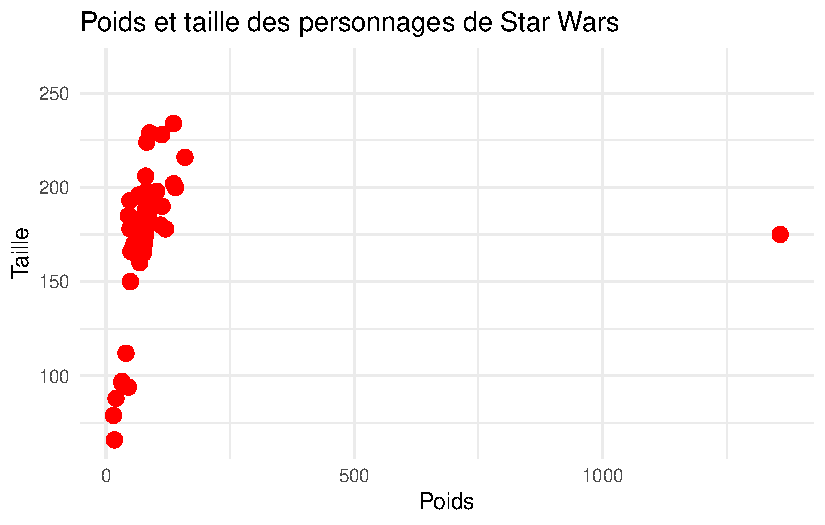
\includegraphics{chapitre_6_files/figure-pdf/unnamed-chunk-2-1.pdf}

\subsection{Pour visualiser les
régressions}\label{pour-visualiser-les-ruxe9gressions}

Lorsque l'on souhaite aller au-delà des analyses descriptives, il
devient pertinent de recourir aux modèles de régression. Si la fonction
\texttt{summary(model)} offre une manière simple et rapide d'obtenir un
aperçu d'un modèle, ses limites se manifestent lorsqu'il s'agit de
visualiser et de comparer plusieurs modèles ou encore de les présenter
de manière claire à une équipe ou dans le cadre d'une publication
scientifique. La section suivante du chapitre introduira divers outils
qui facilitent la visualisation, la comparaison et la présentation
efficace de nos modèles de régression.

\begin{tcolorbox}[enhanced jigsaw, rightrule=.15mm, colframe=quarto-callout-note-color-frame, breakable, bottomrule=.15mm, colback=white, toprule=.15mm, leftrule=.75mm, toptitle=1mm, opacityback=0, coltitle=black, colbacktitle=quarto-callout-note-color!10!white, bottomtitle=1mm, left=2mm, arc=.35mm, title=\textcolor{quarto-callout-note-color}{\faInfo}\hspace{0.5em}{Note}, titlerule=0mm, opacitybacktitle=0.6]

Le manuel d'instructions de cette section restera volontairement bref et
concis en raison de l'abondante documentation déjà existante sur ces
outils. L'objectif ici est de les centraliser en un seul endroit.

\end{tcolorbox}

\subsubsection{\texorpdfstring{Le package
\texttt{stargazer}}{Le package stargazer}}\label{le-package-stargazer}

Le package \texttt{stargazer} est un package qui permet de générer des
tableaux de régression de manière simple et efficace. Selon son auteur,
Marek Hlavac, ce package excelle dans trois aspects : sa facilité
d'utilisation, la diversité des modèles supportés et son esthétisme
(\textbf{hlavac22?}). Bien que nous soyons partiellement d'accord avec
ces propos et que \texttt{stargazer} réponde effectivement à ces trois
aspects, nous estimons que le package \texttt{modelsummary}
(Section~\ref{sec-model-summary}) surpasse \texttt{stargazer} dans
chacun de ces domaines.

Voici une façon standard d'utiliser \texttt{stargazer} pour créer un
tableau de deux modèles de régression:

\begin{Shaded}
\begin{Highlighting}[]
\CommentTok{\# Il faut premièrement installer et importer le package stargazer si ce n\textquotesingle{}est}
\CommentTok{\#   pas déjà fait.}

\CommentTok{\# install.packages("stargazer") \# pour installer}

\FunctionTok{library}\NormalTok{(stargazer) }\CommentTok{\# importer le package}

\DocumentationTok{\#\# Créer deux modèles de régression}
\NormalTok{mod\_lm }\OtherTok{\textless{}{-}} \FunctionTok{lm}\NormalTok{(mpg }\SpecialCharTok{\textasciitilde{}}\NormalTok{ hp }\SpecialCharTok{+}\NormalTok{ wt, }\AttributeTok{data =}\NormalTok{ mtcars)}
\NormalTok{mod\_glm }\OtherTok{\textless{}{-}} \FunctionTok{glm}\NormalTok{(vs }\SpecialCharTok{\textasciitilde{}}\NormalTok{ hp }\SpecialCharTok{+}\NormalTok{ wt }\SpecialCharTok{+}\NormalTok{ drat, }\AttributeTok{data =}\NormalTok{ mtcars, }\AttributeTok{family =} \FunctionTok{binomial}\NormalTok{())}

\FunctionTok{stargazer}\NormalTok{(}
\NormalTok{  mod\_lm,}
\NormalTok{  mod\_glm,}
  \AttributeTok{type =} \StringTok{"text"}\NormalTok{,}
  \AttributeTok{title =} \StringTok{"Tableau de régression des modèles"}
\NormalTok{  )}
\end{Highlighting}
\end{Shaded}

\begin{verbatim}

Tableau de régression des modèles
===================================================
                          Dependent variable:      
                    -------------------------------
                             mpg              vs   
                             OLS           logistic
                             (1)             (2)   
---------------------------------------------------
hp                        -0.032***        -0.104**
                           (0.009)         (0.050) 
                                                   
wt                        -3.878***         0.860  
                           (0.633)         (1.299) 
                                                   
drat                                        -1.625 
                                           (2.073) 
                                                   
Constant                  37.227***         16.030 
                           (1.599)         (11.974)
                                                   
---------------------------------------------------
Observations                  32              32   
R2                          0.827                  
Adjusted R2                 0.815                  
Log Likelihood                              -7.698 
Akaike Inf. Crit.                           23.395 
Residual Std. Error    2.593 (df = 29)             
F Statistic         69.211*** (df = 2; 29)         
===================================================
Note:                   *p<0.1; **p<0.05; ***p<0.01
\end{verbatim}

Alors que cette sortie texte est intéressante afin de rapidement
visualiser différents modèles de régression, \texttt{stargazer} offre
également l'option de transformer ces modèles en \texttt{latex} avec
l'argument \texttt{type}:

\begin{Shaded}
\begin{Highlighting}[]
\FunctionTok{stargazer}\NormalTok{(}
\NormalTok{  mod\_lm,}
\NormalTok{  mod\_glm,}
  \AttributeTok{type =} \StringTok{"latex"}\NormalTok{,}
  \AttributeTok{title =} \StringTok{"Tableau de régression des modèles"}
\NormalTok{  )}
\end{Highlighting}
\end{Shaded}

\begin{verbatim}

% Table created by stargazer v.5.2.3 by Marek Hlavac, Social Policy Institute. E-mail: marek.hlavac at gmail.com
% Date and time: Wed, Nov 13, 2024 - 03:43:01 PM
\begin{table}[!htbp] \centering 
  \caption{Tableau de régression des modèles} 
  \label{} 
\begin{tabular}{@{\extracolsep{5pt}}lcc} 
\\[-1.8ex]\hline 
\hline \\[-1.8ex] 
 & \multicolumn{2}{c}{\textit{Dependent variable:}} \\ 
\cline{2-3} 
\\[-1.8ex] & mpg & vs \\ 
\\[-1.8ex] & \textit{OLS} & \textit{logistic} \\ 
\\[-1.8ex] & (1) & (2)\\ 
\hline \\[-1.8ex] 
 hp & $-$0.032$^{***}$ & $-$0.104$^{**}$ \\ 
  & (0.009) & (0.050) \\ 
  & & \\ 
 wt & $-$3.878$^{***}$ & 0.860 \\ 
  & (0.633) & (1.299) \\ 
  & & \\ 
 drat &  & $-$1.625 \\ 
  &  & (2.073) \\ 
  & & \\ 
 Constant & 37.227$^{***}$ & 16.030 \\ 
  & (1.599) & (11.974) \\ 
  & & \\ 
\hline \\[-1.8ex] 
Observations & 32 & 32 \\ 
R$^{2}$ & 0.827 &  \\ 
Adjusted R$^{2}$ & 0.815 &  \\ 
Log Likelihood &  & $-$7.698 \\ 
Akaike Inf. Crit. &  & 23.395 \\ 
Residual Std. Error & 2.593 (df = 29) &  \\ 
F Statistic & 69.211$^{***}$ (df = 2; 29) &  \\ 
\hline 
\hline \\[-1.8ex] 
\textit{Note:}  & \multicolumn{2}{r}{$^{*}$p$<$0.1; $^{**}$p$<$0.05; $^{***}$p$<$0.01} \\ 
\end{tabular} 
\end{table} 
\end{verbatim}

Alors que cette sortie est moins compréhensible qu'avec
\texttt{type\ =\ "text"}, elle a l'avantage de pouvoir être copiée et
collée dans un fichier .tex et ainsi présenter le tableau dans un
article par exemple. Une autre option est possible avec
\texttt{type\ =\ "html"} afin d'inclure la table de régression dans un
code html (à des fins de lisibilité, nous n'avons pas présenté la sortie
de cette commande. Essayez-le dans votre environnement de
programmation!):

\begin{Shaded}
\begin{Highlighting}[]
\FunctionTok{stargazer}\NormalTok{(}
\NormalTok{  mod\_lm,}
\NormalTok{  mod\_glm,}
  \AttributeTok{type =} \StringTok{"html"}\NormalTok{,}
  \AttributeTok{title =} \StringTok{"Tableau de régression des modèles"}
\NormalTok{  )}
\end{Highlighting}
\end{Shaded}

Bien qu'il existe des milliers de façons de personnaliser son tableau de
régression avec \texttt{stargazer}, nous vous invitons à consulter la
documentation du package (\textbf{hlavac22?}) ainsi que différents blogs
en ligne afin de personnaliser votre tableau comme vous le voulez.

\subsubsection{\texorpdfstring{\texttt{modelsummary}}{modelsummary}}\label{sec-model-summary}

Le package \texttt{modelsummary} (Arel-Bundock, 2022), développé dans le
même but que \texttt{stargazer}, est une nette amélioration au package
\texttt{stargazer} selon l'avis des auteurs du chapitre: il est encore
plus facile d'utilisation, supporte une grande variété de modèles et se
connecte à divers autres outils afin de contrôler l'esthétisme de son
résultat. De plus, la documentation officielle du package est beaucoup
plus abondante et claire. Finalement, le package est plus intuitif à
utiliser.

Tout comme \texttt{stargazer}, il faut commencer en créant un modèle de
régression. Puis, il suffit d'inclure les modèles dans la fonction
\texttt{modelsummary}:

\begin{Shaded}
\begin{Highlighting}[]
\CommentTok{\# Il faut premièrement installer et importer le package modelsummary si ce}
\CommentTok{\#   n\textquotesingle{}est pas déjà fait.}

\CommentTok{\# install.packages("modelsummary") \# pour installer}

\FunctionTok{library}\NormalTok{(modelsummary) }\CommentTok{\# importer le package}
\end{Highlighting}
\end{Shaded}

\begin{Shaded}
\begin{Highlighting}[]
\DocumentationTok{\#\# Créer deux modèles de régression}
\NormalTok{mod\_lm }\OtherTok{\textless{}{-}} \FunctionTok{lm}\NormalTok{(mpg }\SpecialCharTok{\textasciitilde{}}\NormalTok{ hp }\SpecialCharTok{+}\NormalTok{ wt, }\AttributeTok{data =}\NormalTok{ mtcars)}
\NormalTok{mod\_glm }\OtherTok{\textless{}{-}} \FunctionTok{glm}\NormalTok{(vs }\SpecialCharTok{\textasciitilde{}}\NormalTok{ hp }\SpecialCharTok{+}\NormalTok{ wt }\SpecialCharTok{+}\NormalTok{ drat, }\AttributeTok{data =}\NormalTok{ mtcars, }\AttributeTok{family =} \FunctionTok{binomial}\NormalTok{())}

\DocumentationTok{\#\# Utiliser modelsummary pour créer un tableau de deux modèles de régression}
\FunctionTok{modelsummary}\NormalTok{(}
  \FunctionTok{list}\NormalTok{(}
    \StringTok{"Model 1"} \OtherTok{=}\NormalTok{ mod\_lm,}
    \StringTok{"Model 2"} \OtherTok{=}\NormalTok{ mod\_glm}
\NormalTok{    ),}
    \AttributeTok{stars =} \ConstantTok{TRUE}\NormalTok{,}
    \AttributeTok{output =} \StringTok{"markdown"}
\NormalTok{  )}
\end{Highlighting}
\end{Shaded}

\begin{table}
\centering
\begin{talltblr}[         %% tabularray outer open
entry=none,label=none,
note{}={+ p < 0.1, * p < 0.05, ** p < 0.01, *** p < 0.001},
]                     %% tabularray outer close
{                     %% tabularray inner open
colspec={Q[]Q[]Q[]},
column{1}={halign=l,},
column{2}={halign=c,},
column{3}={halign=c,},
hline{10}={1,2,3}{solid, 0.05em, black},
}                     %% tabularray inner close
\toprule
& Model 1 & Model 2 \\ \midrule %% TinyTableHeader
(Intercept) & 37.227*** & 16.030   \\
& (1.599)   & (11.974) \\
hp          & -0.032**  & -0.104*  \\
& (0.009)   & (0.050)  \\
wt          & -3.878*** & 0.860    \\
& (0.633)   & (1.299)  \\
drat        &           & -1.625   \\
&           & (2.073)  \\
Num.Obs.    & 32        & 32       \\
R2          & 0.827     &          \\
R2 Adj.     & 0.815     &          \\
AIC         & 156.7     & 23.4     \\
BIC         & 162.5     & 29.3     \\
Log.Lik.    & -74.326   & -7.698   \\
F           & 69.211    & 1.892    \\
RMSE        & 2.47      & 0.29     \\
\bottomrule
\end{talltblr}
\end{table}

Tout comme \texttt{stargazer}, \texttt{modelsummary} offre également
plusieurs options de sortie avec l'argument \texttt{output}. Cependant,
\texttt{modelsummary} en supporte plus, comme \texttt{kableExtra},
\texttt{html}, \texttt{latex} et bien d'autres formats.

Nous vous invitons à consulter la documentation du package
\texttt{modelsummary} (Arel-Bundock, 2022) pour plus d'informations sur
la personnalisation de vos tableaux de régression.

\subsubsection{\texorpdfstring{\texttt{marginaleffects}}{marginaleffects}}\label{marginaleffects}

Les tableaux de régression présentent souvent les résultats des modèles
de manière brute et difficile à interpréter. Une approche plus intuitive
pour visualiser et comprendre ces modèles consiste à utiliser les
prédictions qu'ils génèrent, puis à interpréter l'impact des variables
indépendantes sur la variable dépendante. Bien que cette démarche puisse
être complexe et fastidieuse à réaliser avec les fonctions de base de R
ou Python, le package R \texttt{marginaleffects} a été spécifiquement
conçu pour simplifier cette tâche et rendre ces analyses plus
accessibles (\textbf{arel-bundock?}).

La première étape est de faire son modèle comme on le fait
habituellement:

\begin{Shaded}
\begin{Highlighting}[]
\CommentTok{\# Il faut premièrement installer et importer le package marginaleffects si}
\CommentTok{\#  ce n\textquotesingle{}est pas déjà fait.}

\CommentTok{\# install.packages("marginaleffects") \# pour installer}

\FunctionTok{library}\NormalTok{(marginaleffects) }\CommentTok{\# importer le package}

\DocumentationTok{\#\# Créer un modèle de régression}
\NormalTok{mod\_lm }\OtherTok{\textless{}{-}} \FunctionTok{lm}\NormalTok{(mpg }\SpecialCharTok{\textasciitilde{}}\NormalTok{ hp }\SpecialCharTok{+}\NormalTok{ wt }\SpecialCharTok{+}\NormalTok{ drat, }\AttributeTok{data =}\NormalTok{ mtcars)}
\end{Highlighting}
\end{Shaded}

Ensuite, il est nécessaire de créer une grille où notre variable
indépendante d'intérêt varie tandis que les autres variables restent
constantes. Prenons, par exemple, le cas où nous souhaitons estimer et
interpréter l'effet de \texttt{hp} sur \texttt{mpg}. Pour ce faire, nous
construisons une \texttt{dataframe} représentant une grille de
différents niveaux de \texttt{hp}, tout en maintenant les variables
\texttt{wt} et \texttt{drat} constantes. Cela nous permet d'isoler
l'effet spécifique de \texttt{hp} et d'explorer son impact sur la
variable dépendante \texttt{mpg}. La première sous-étape ici est de
comprendre les différentes valeurs que peut prendre notre variable
d'intérêt, \texttt{hp}:

\begin{Shaded}
\begin{Highlighting}[]
\FunctionTok{table}\NormalTok{(mtcars}\SpecialCharTok{$}\NormalTok{hp)}
\end{Highlighting}
\end{Shaded}

\begin{verbatim}

 52  62  65  66  91  93  95  97 105 109 110 113 123 150 175 180 205 215 230 245 
  1   1   1   2   1   1   1   1   1   1   3   1   2   2   3   3   1   1   1   2 
264 335 
  1   1 
\end{verbatim}

\begin{Shaded}
\begin{Highlighting}[]
\FunctionTok{hist}\NormalTok{(mtcars}\SpecialCharTok{$}\NormalTok{hp)}
\end{Highlighting}
\end{Shaded}

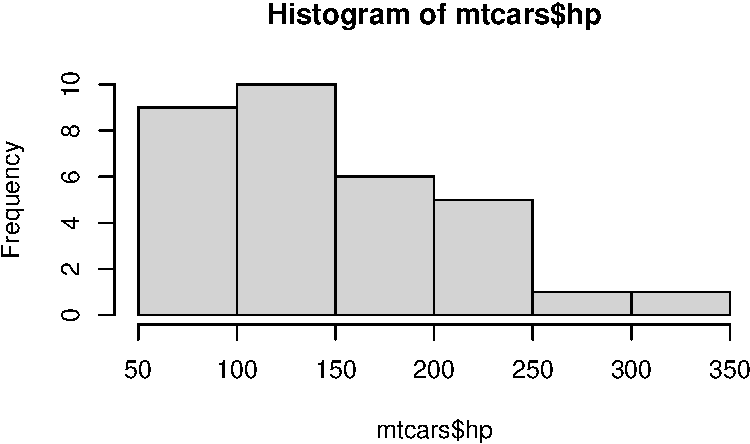
\includegraphics{chapitre_6_files/figure-pdf/unnamed-chunk-9-1.pdf}

Comme on peut voir, la variable \texttt{hp} peut prendre n'importe
quelle valeur numérique entre 52 et 335. La prochaine étape est de
construire notre grille en utilisant la fonction \texttt{datagrid} du
package:

\begin{Shaded}
\begin{Highlighting}[]
\NormalTok{grille }\OtherTok{\textless{}{-}}\NormalTok{ marginaleffects}\SpecialCharTok{::}\FunctionTok{datagrid}\NormalTok{(}
      \AttributeTok{model =}\NormalTok{ mod\_lm,}
      \AttributeTok{hp =} \FunctionTok{c}\NormalTok{(}\DecValTok{50}\NormalTok{, }\DecValTok{100}\NormalTok{, }\DecValTok{150}\NormalTok{, }\DecValTok{200}\NormalTok{, }\DecValTok{250}\NormalTok{, }\DecValTok{300}\NormalTok{, }\DecValTok{350}\NormalTok{)}
\NormalTok{)}

\FunctionTok{print}\NormalTok{(grille)}
\end{Highlighting}
\end{Shaded}

\begin{verbatim}
       wt     drat  hp rowid
1 3.21725 3.596563  50     1
2 3.21725 3.596563 100     2
3 3.21725 3.596563 150     3
4 3.21725 3.596563 200     4
5 3.21725 3.596563 250     5
6 3.21725 3.596563 300     6
7 3.21725 3.596563 350     7
\end{verbatim}

Comme on peut le voir, la variable \texttt{grille} est maintenant une
\texttt{dataframe} qui contient 7 rangées. Les variables \texttt{wt} et
\texttt{drat} conservent la même valeur dans chaque rangée ; la variable
\texttt{hp} prend cependant les 7 valeurs que nous avons définies.

La prochaine étape est celle de prédire notre modèle sur ces données en
utilisant la fonction \texttt{predictions} du package:

\begin{Shaded}
\begin{Highlighting}[]
\NormalTok{predictions }\OtherTok{\textless{}{-}}\NormalTok{ marginaleffects}\SpecialCharTok{::}\FunctionTok{predictions}\NormalTok{(}
      \AttributeTok{model =}\NormalTok{ mod\_lm,}
      \DocumentationTok{\#\# Ici, on dit à R de prédire notre modèle sur nos nouvelles données}
      \DocumentationTok{\#\#  ie: grille}
      \AttributeTok{newdata =}\NormalTok{ grille}
\NormalTok{)}

\FunctionTok{print}\NormalTok{(}\FunctionTok{as.data.frame}\NormalTok{(predictions))}
\end{Highlighting}
\end{Shaded}

\begin{verbatim}
  rowid estimate std.error statistic       p.value   s.value  conf.low
1     1 23.20690 0.9744661 23.814991 2.335875e-125 414.01705 21.296984
2     2 21.59538 0.6153142 35.096512 7.619361e-270 893.99092 20.389388
3     3 19.98386 0.4537357 44.042960  0.000000e+00       Inf 19.094556
4     4 18.37234 0.6567937 27.972773 3.484472e-172 569.57069 17.085050
5     5 16.76082 1.0271889 16.317175  7.450453e-60 196.41836 14.747568
6     6 15.14930 1.4412127 10.511496  7.647059e-26  83.43523 12.324576
7     7 13.53778 1.8701090  7.239033  4.518950e-13  41.00908  9.872435
  conf.high      wt     drat  hp mpg
1  25.11682 3.21725 3.596563  50  21
2  22.80138 3.21725 3.596563 100  21
3  20.87317 3.21725 3.596563 150  21
4  19.65963 3.21725 3.596563 200  21
5  18.77407 3.21725 3.596563 250  21
6  17.97403 3.21725 3.596563 300  21
7  17.20313 3.21725 3.596563 350  21
\end{verbatim}

La \texttt{dataframe} predictions contient maintenant des informations
très intéressantes:

\begin{itemize}
\tightlist
\item
  \texttt{estimate}: la valeur prédite de \texttt{mpg} pour cette
  observation.
\item
  \texttt{conf.low}: la borne inférieure de l'intervalle de confiance de
  la prédiction pour cette observation.
\item
  \texttt{conf.high}: la borne supérieure de l'intervalle de confiance
  de la prédiction pour cette observation.
\item
  \texttt{hp}, \texttt{wt} et \texttt{drat}: les valeurs que prennent
  nos variables indépendantes pour arriver à cette prédiction. Encore
  une fois, on peut remarquer comment \texttt{hp} varie, mais pas
  \texttt{wt} et \texttt{drat}.
\end{itemize}

Nous pouvons maintenant utiliser \texttt{predictions} pour construire un
graphique qui nous permet d'interpréter l'effet de \texttt{hp} sur
\texttt{mpg} à l'intérieur de notre modèle en contrôlant pour
\texttt{wt} et \texttt{drat} en utilisant le package \texttt{ggplot2}:

\begin{Shaded}
\begin{Highlighting}[]
\FunctionTok{ggplot}\NormalTok{(predictions, }\FunctionTok{aes}\NormalTok{(}\AttributeTok{x =}\NormalTok{ hp, }\AttributeTok{y =}\NormalTok{ estimate)) }\SpecialCharTok{+}
      \FunctionTok{geom\_point}\NormalTok{() }\SpecialCharTok{+}
      \FunctionTok{geom\_linerange}\NormalTok{(}\FunctionTok{aes}\NormalTok{(}\AttributeTok{ymin =}\NormalTok{ conf.low, }\AttributeTok{ymax =}\NormalTok{ conf.high))}
\end{Highlighting}
\end{Shaded}

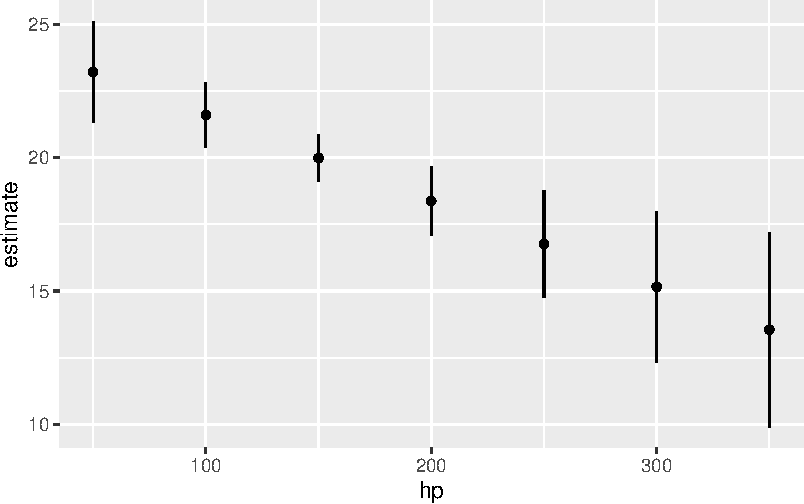
\includegraphics{chapitre_6_files/figure-pdf/unnamed-chunk-12-1.pdf}

Et voilà, le tour est joué ! Il existe de nombreuses manières de
présenter et d'adapter ce graphique selon vos besoins. Il est également
important de souligner que le package \texttt{marginaleffects} est
extrêmement polyvalent, prenant en charge des centaines de types de
modèles et offrant une large gamme de fonctionnalités. Pour découvrir
toutes ses possibilités, nous vous invitons à consulter la documentation
officielle du package (\textbf{arel-bundock?}).

\subsection{Aller plus loin: La visualisation interactive des
données}\label{aller-plus-loin-la-visualisation-interactive-des-donnuxe9es}

Si jusqu'à présent la visualisation des données a été présentée comme
une étape servant à exposer les résultats de recherches, elle peut
également être perçue comme un outil précieux pour l'exploration de
données multidimensionnelles. En effet, les visualisations interactives
offrent la possibilité d'explorer et même d'analyser les données
directement à partir des graphiques ou tableaux. Cela permet non
seulement de mieux appréhender la structure des données, mais aussi de
les inspecter plus efficacement, tout en suscitant des questions de
recherche qui auraient pu être négligées autrement (Sievert, 2020).

\subsubsection{Graphiques interactifs}\label{graphiques-interactifs}

Les graphiques interactifs permettent une exploration dynamique des
données, offrant aux utilisateurs la possibilité de zoomer, survoler des
points pour obtenir plus d'informations, et d'examiner les relations
entre variables de manière plus intuitive. En R, les packages
\texttt{ggplotly} et \texttt{plotly} permettent de créer facilement des
graphiques interactifs à partir de visualisations statiques.

\begin{tcolorbox}[enhanced jigsaw, rightrule=.15mm, colframe=quarto-callout-note-color-frame, breakable, bottomrule=.15mm, colback=white, toprule=.15mm, leftrule=.75mm, toptitle=1mm, opacityback=0, coltitle=black, colbacktitle=quarto-callout-note-color!10!white, bottomtitle=1mm, left=2mm, arc=.35mm, title=\textcolor{quarto-callout-note-color}{\faInfo}\hspace{0.5em}{Note}, titlerule=0mm, opacitybacktitle=0.6]

Note: Le rendu de graphiques interactifs n'est pas possible dans un
document PDF. Par conséquent, seuls les codes sont fournis ci-dessous.
Vous pouvez essayer ces codes dans votre environnement de développement
pour voir le résultat.

\end{tcolorbox}

\paragraph{\texorpdfstring{Exemple avec
\texttt{ggplotly}}{Exemple avec ggplotly}}\label{exemple-avec-ggplotly}

\texttt{ggplotly} permet de transformer un graphique \texttt{ggplot2} en
une visualisation interactive.

\begin{Shaded}
\begin{Highlighting}[]
\FunctionTok{library}\NormalTok{(ggplot2)}
\FunctionTok{library}\NormalTok{(plotly)}
\end{Highlighting}
\end{Shaded}

\begin{Shaded}
\begin{Highlighting}[]
\CommentTok{\# Ce package, webshot2, peut être nécessaire pour visualiser}
\CommentTok{\#  des graphiques interactifs}

\CommentTok{\#install.packages("webshot2")}

\CommentTok{\# Création d\textquotesingle{}un graphique ggplot}
\NormalTok{p }\OtherTok{\textless{}{-}} \FunctionTok{ggplot}\NormalTok{(mtcars, }\FunctionTok{aes}\NormalTok{(}\AttributeTok{x =}\NormalTok{ hp, }\AttributeTok{y =}\NormalTok{ mpg)) }\SpecialCharTok{+}
  \FunctionTok{geom\_point}\NormalTok{() }\SpecialCharTok{+}
  \FunctionTok{labs}\NormalTok{(}\AttributeTok{title =} \StringTok{"Effet de hp sur mpg"}\NormalTok{)}

\CommentTok{\# Transformation en graphique interactif}
\FunctionTok{ggplotly}\NormalTok{(p)}
\end{Highlighting}
\end{Shaded}

Et voici un exemple avec \texttt{plotly}, un package qui n'emprunte pas
la grammaire de \texttt{ggplot2}:

\begin{Shaded}
\begin{Highlighting}[]
\CommentTok{\# Création d\textquotesingle{}un graphique interactif avec plotly}
\NormalTok{fig }\OtherTok{\textless{}{-}} \FunctionTok{plot\_ly}\NormalTok{(}
  \AttributeTok{data =}\NormalTok{ mtcars,}
  \AttributeTok{x =} \SpecialCharTok{\textasciitilde{}}\NormalTok{hp, }\AttributeTok{y =} \SpecialCharTok{\textasciitilde{}}\NormalTok{mpg,}
  \AttributeTok{type =} \StringTok{\textquotesingle{}scatter\textquotesingle{}}\NormalTok{,}
  \AttributeTok{mode =} \StringTok{\textquotesingle{}markers\textquotesingle{}}
\NormalTok{  ) }\SpecialCharTok{\%\textgreater{}\%}
  \FunctionTok{layout}\NormalTok{(}\AttributeTok{title =} \StringTok{"Effet de hp sur mpg"}\NormalTok{)}

\NormalTok{fig}
\end{Highlighting}
\end{Shaded}

Nous vous recommandons vivement de consulter la documentation officielle
des packages \texttt{plotly} et \texttt{ggplotly} pour découvrir toutes
les options et fonctionnalités disponibles, afin d'enrichir vos
graphiques interactifs.

\subsubsection{Tableaux interactifs}\label{tableaux-interactifs}

Les tableaux interactifs sont très utiles pour rendre la présentation
des données plus engageante et informative. Les fonctions
\texttt{kable()} et \texttt{kableExtra} permettent de créer des tableaux
élégants et interactifs directement dans R.

\paragraph{\texorpdfstring{Exemple avec
\texttt{kable()}}{Exemple avec kable()}}\label{exemple-avec-kable}

La fonction \texttt{kable()} de \texttt{knitr} permet de transformer un
dataframe en un tableau bien formaté.

\begin{Shaded}
\begin{Highlighting}[]
\FunctionTok{library}\NormalTok{(knitr)}

\CommentTok{\# Création d\textquotesingle{}un tableau avec kable}
\FunctionTok{kable}\NormalTok{(}\FunctionTok{head}\NormalTok{(mtcars), }\AttributeTok{caption =} \StringTok{"Exemple de tableau avec kable"}\NormalTok{)}
\end{Highlighting}
\end{Shaded}

\begin{longtable}[]{@{}
  >{\raggedright\arraybackslash}p{(\columnwidth - 22\tabcolsep) * \real{0.2609}}
  >{\raggedleft\arraybackslash}p{(\columnwidth - 22\tabcolsep) * \real{0.0725}}
  >{\raggedleft\arraybackslash}p{(\columnwidth - 22\tabcolsep) * \real{0.0580}}
  >{\raggedleft\arraybackslash}p{(\columnwidth - 22\tabcolsep) * \real{0.0725}}
  >{\raggedleft\arraybackslash}p{(\columnwidth - 22\tabcolsep) * \real{0.0580}}
  >{\raggedleft\arraybackslash}p{(\columnwidth - 22\tabcolsep) * \real{0.0725}}
  >{\raggedleft\arraybackslash}p{(\columnwidth - 22\tabcolsep) * \real{0.0870}}
  >{\raggedleft\arraybackslash}p{(\columnwidth - 22\tabcolsep) * \real{0.0870}}
  >{\raggedleft\arraybackslash}p{(\columnwidth - 22\tabcolsep) * \real{0.0435}}
  >{\raggedleft\arraybackslash}p{(\columnwidth - 22\tabcolsep) * \real{0.0435}}
  >{\raggedleft\arraybackslash}p{(\columnwidth - 22\tabcolsep) * \real{0.0725}}
  >{\raggedleft\arraybackslash}p{(\columnwidth - 22\tabcolsep) * \real{0.0725}}@{}}
\caption{Exemple de tableau avec kable}\tabularnewline
\toprule\noalign{}
\begin{minipage}[b]{\linewidth}\raggedright
\end{minipage} & \begin{minipage}[b]{\linewidth}\raggedleft
mpg
\end{minipage} & \begin{minipage}[b]{\linewidth}\raggedleft
cyl
\end{minipage} & \begin{minipage}[b]{\linewidth}\raggedleft
disp
\end{minipage} & \begin{minipage}[b]{\linewidth}\raggedleft
hp
\end{minipage} & \begin{minipage}[b]{\linewidth}\raggedleft
drat
\end{minipage} & \begin{minipage}[b]{\linewidth}\raggedleft
wt
\end{minipage} & \begin{minipage}[b]{\linewidth}\raggedleft
qsec
\end{minipage} & \begin{minipage}[b]{\linewidth}\raggedleft
vs
\end{minipage} & \begin{minipage}[b]{\linewidth}\raggedleft
am
\end{minipage} & \begin{minipage}[b]{\linewidth}\raggedleft
gear
\end{minipage} & \begin{minipage}[b]{\linewidth}\raggedleft
carb
\end{minipage} \\
\midrule\noalign{}
\endfirsthead
\toprule\noalign{}
\begin{minipage}[b]{\linewidth}\raggedright
\end{minipage} & \begin{minipage}[b]{\linewidth}\raggedleft
mpg
\end{minipage} & \begin{minipage}[b]{\linewidth}\raggedleft
cyl
\end{minipage} & \begin{minipage}[b]{\linewidth}\raggedleft
disp
\end{minipage} & \begin{minipage}[b]{\linewidth}\raggedleft
hp
\end{minipage} & \begin{minipage}[b]{\linewidth}\raggedleft
drat
\end{minipage} & \begin{minipage}[b]{\linewidth}\raggedleft
wt
\end{minipage} & \begin{minipage}[b]{\linewidth}\raggedleft
qsec
\end{minipage} & \begin{minipage}[b]{\linewidth}\raggedleft
vs
\end{minipage} & \begin{minipage}[b]{\linewidth}\raggedleft
am
\end{minipage} & \begin{minipage}[b]{\linewidth}\raggedleft
gear
\end{minipage} & \begin{minipage}[b]{\linewidth}\raggedleft
carb
\end{minipage} \\
\midrule\noalign{}
\endhead
\bottomrule\noalign{}
\endlastfoot
Mazda RX4 & 21.0 & 6 & 160 & 110 & 3.90 & 2.620 & 16.46 & 0 & 1 & 4 &
4 \\
Mazda RX4 Wag & 21.0 & 6 & 160 & 110 & 3.90 & 2.875 & 17.02 & 0 & 1 & 4
& 4 \\
Datsun 710 & 22.8 & 4 & 108 & 93 & 3.85 & 2.320 & 18.61 & 1 & 1 & 4 &
1 \\
Hornet 4 Drive & 21.4 & 6 & 258 & 110 & 3.08 & 3.215 & 19.44 & 1 & 0 & 3
& 1 \\
Hornet Sportabout & 18.7 & 8 & 360 & 175 & 3.15 & 3.440 & 17.02 & 0 & 0
& 3 & 2 \\
Valiant & 18.1 & 6 & 225 & 105 & 2.76 & 3.460 & 20.22 & 1 & 0 & 3 & 1 \\
\end{longtable}

\subsubsection{\texorpdfstring{Exemple avec
\texttt{kableExtra}}{Exemple avec kableExtra}}\label{exemple-avec-kableextra}

Le package kableExtra permet de personnaliser et d'enrichir les tableaux
créés avec kable(), notamment en ajoutant des options interactives comme
des couleurs ou des styles.

\begin{Shaded}
\begin{Highlighting}[]
\FunctionTok{library}\NormalTok{(kableExtra)}
\end{Highlighting}
\end{Shaded}

\begin{Shaded}
\begin{Highlighting}[]
\CommentTok{\# Création d\textquotesingle{}un tableau interactif avec kableExtra}
\FunctionTok{kable}\NormalTok{(}
  \FunctionTok{head}\NormalTok{(mtcars),}
  \AttributeTok{caption =} \StringTok{"Exemple de tableau avec la colonne hp colorée en rouge"}
\NormalTok{  ) }\SpecialCharTok{\%\textgreater{}\%}
  \FunctionTok{kable\_styling}\NormalTok{(}\AttributeTok{bootstrap\_options =} \FunctionTok{c}\NormalTok{(}\StringTok{"striped"}\NormalTok{, }\StringTok{"hover"}\NormalTok{, }\StringTok{"condensed"}\NormalTok{)) }\SpecialCharTok{\%\textgreater{}\%}
  \FunctionTok{column\_spec}\NormalTok{(}\DecValTok{5}\NormalTok{, }\AttributeTok{background =} \StringTok{"red"}\NormalTok{)}
\end{Highlighting}
\end{Shaded}

\begin{longtable}[t]{lrrr>{}rrrrrrrr}
\caption{Exemple de tableau avec la colonne hp colorée en rouge}\\
\toprule
 & mpg & cyl & disp & hp & drat & wt & qsec & vs & am & gear & carb\\
\midrule
Mazda RX4 & 21.0 & 6 & 160 & \cellcolor{red}{110} & 3.90 & 2.620 & 16.46 & 0 & 1 & 4 & 4\\
Mazda RX4 Wag & 21.0 & 6 & 160 & \cellcolor{red}{110} & 3.90 & 2.875 & 17.02 & 0 & 1 & 4 & 4\\
Datsun 710 & 22.8 & 4 & 108 & \cellcolor{red}{93} & 3.85 & 2.320 & 18.61 & 1 & 1 & 4 & 1\\
Hornet 4 Drive & 21.4 & 6 & 258 & \cellcolor{red}{110} & 3.08 & 3.215 & 19.44 & 1 & 0 & 3 & 1\\
Hornet Sportabout & 18.7 & 8 & 360 & \cellcolor{red}{175} & 3.15 & 3.440 & 17.02 & 0 & 0 & 3 & 2\\
\addlinespace
Valiant & 18.1 & 6 & 225 & \cellcolor{red}{105} & 2.76 & 3.460 & 20.22 & 1 & 0 & 3 & 1\\
\bottomrule
\end{longtable}

\subsubsection{Applications interactives avec
Shiny}\label{applications-interactives-avec-shiny}

\texttt{shiny} est un package R puissant qui permet de créer des
applications web interactives sans avoir besoin de compétences avancées
en développement web. Il permet de relier facilement des données, des
visualisations et des contrôles interactifs, rendant les analyses
accessibles à un large public via une interface web.

\paragraph{\texorpdfstring{Exemple de base avec
\texttt{shiny}}{Exemple de base avec shiny}}\label{exemple-de-base-avec-shiny}

Voici un exemple simple d'application \texttt{shiny} où l'utilisateur
peut sélectionner une variable pour tracer un graphique interactif. Si
le package \texttt{shiny} est installé sur votre poste, vous pouvez
simplement copier ce code dans un script R sous RStudio, puis lancer
l'application web directement.

\begin{Shaded}
\begin{Highlighting}[]
\FunctionTok{library}\NormalTok{(shiny)}
\FunctionTok{library}\NormalTok{(ggplot2)}

\CommentTok{\# Interface utilisateur}
\NormalTok{ui }\OtherTok{\textless{}{-}} \FunctionTok{fluidPage}\NormalTok{(}
  \FunctionTok{titlePanel}\NormalTok{(}\StringTok{"Exemple d\textquotesingle{}application Shiny"}\NormalTok{),}
  \FunctionTok{sidebarLayout}\NormalTok{(}
    \FunctionTok{sidebarPanel}\NormalTok{(}
      \FunctionTok{selectInput}\NormalTok{(}\StringTok{"var"}\NormalTok{, }\StringTok{"Choisir une variable:"}\NormalTok{,}
                  \AttributeTok{choices =} \FunctionTok{names}\NormalTok{(mtcars))}
\NormalTok{    ),}
    \FunctionTok{mainPanel}\NormalTok{(}
      \FunctionTok{plotOutput}\NormalTok{(}\StringTok{"plot"}\NormalTok{)}
\NormalTok{    )}
\NormalTok{  )}
\NormalTok{)}

\CommentTok{\# Serveur}
\NormalTok{server }\OtherTok{\textless{}{-}} \ControlFlowTok{function}\NormalTok{(input, output) \{}
\NormalTok{  output}\SpecialCharTok{$}\NormalTok{plot }\OtherTok{\textless{}{-}} \FunctionTok{renderPlot}\NormalTok{(\{}
    \FunctionTok{ggplot}\NormalTok{(mtcars, }\FunctionTok{aes\_string}\NormalTok{(}\AttributeTok{x =}\NormalTok{ input}\SpecialCharTok{$}\NormalTok{var, }\AttributeTok{y =} \StringTok{"mpg"}\NormalTok{)) }\SpecialCharTok{+}
      \FunctionTok{geom\_point}\NormalTok{() }\SpecialCharTok{+}
      \FunctionTok{labs}\NormalTok{(}\AttributeTok{title =} \FunctionTok{paste}\NormalTok{(}\StringTok{"Effet de"}\NormalTok{, input}\SpecialCharTok{$}\NormalTok{var, }\StringTok{"sur mpg"}\NormalTok{))}
\NormalTok{  \})}
\NormalTok{\}}

\CommentTok{\# Lancement de l\textquotesingle{}application}
\FunctionTok{shinyApp}\NormalTok{(}\AttributeTok{ui =}\NormalTok{ ui, }\AttributeTok{server =}\NormalTok{ server)}
\end{Highlighting}
\end{Shaded}

Cette application simple permet à l'utilisateur de choisir une variable
dans le jeu de données mtcars pour voir son impact sur la consommation
de carburant (\texttt{mpg}), visualisée à travers un graphique
interactif.

Pour explorer davantage les possibilités de \texttt{shiny}, nous vous
recommandons de consulter la documentation officielle du package
\texttt{shiny} ainsi que les forums en ligne qui proposent des exemples
plus complexes et des fonctionnalités avancées pour enrichir vos
applications.

\bookmarksetup{startatroot}

\chapter{Outils de rédaction en sciences sociales numériques: les
langages de balisage}\label{sec-chap7}

En lisant un article scientifique, une page Web ou un curriculum vitæ
professionnel, comme plusieurs lecteurs l'auront sans doute deviné, le
texte n'est pas toujours produit à l'aide d'un logiciel de traitement de
texte comme Microsoft Word, Apple Pages ou LibreOffice Writer. La mise
en page complexe réglée au millimètre près, la qualité des figures et
des tableaux, l'utilisation de gabarits professionnels, le style des
références ou encore la présence d'éléments interactifs sont difficiles
et parfois impossibles à reproduire à l'aide d'un logiciel de traitement
de texte régulier. L'ajout d'extraits de code, de tableaux de régression
ou encore de figures de haute qualité graphique, ainsi que leur
personnalisation, nécessitent une interface particulière.

Pour ces raisons et plusieurs autres, les chercheurs en sciences
sociales font souvent appel aux langages de balisage, ou \emph{markup
languages}. Ceux-ci permettent de produire des documents et pages Web
sans les limitations des logiciels de traitement de texte. Le présent
livre, par exemple, est écrit à l'aide du langage de balisage Markdown
avec l'aide du système de publication Quarto. Les logiciels de
traitement de texte et les langages de balisage font tous partie de la
catégorie des \textbf{outils de rédaction}.

Il est d'ailleurs important de distinguer les langages de balisage des
langages de programmation, qui sont abordés plus en détail dans le
chapitre 2. En effet, ceux-ci sont similaires à certains égards, mais
ont des vocations différentes. Les deux s'appuient sur un langage
informatisé, mais les langages et leurs objectifs diffèrent. Un langage
de programmation définit des processus informatisés alors qu'un langage
de balisage permet d'encoder du contenu de manière à ce que celui-ci
soit lisible tant pour l'humain que pour son ordinateur.

D'entrée de jeu, il peut sembler curieux d'apprendre des langages de
balisage alors que les logiciels de traitement de texte sont nombreux,
simples d'approche et en amélioration constante. Ce chapitre n'a pas
pour objectif de décourager l'utilisation de ces logiciels, qui sont
utiles et même souvent essentiels pour la production rapide de documents
ainsi que pour des tâches de suivi des modifications et de travail avec
des équipes multidisciplinaires. Le chapitre tentera plutôt de démontrer
que la maîtrise des langages de balisage constitue un avantage pour ceux
qui souhaitent s'initier au monde de la recherche académique, même si
quelques difficultés initiales d'apprentissage peuvent se présenter. Il
s'agira de répondre, tour à tour, aux trois grandes questions
suivantes~: \emph{Qu'est-ce qu'un langage de balisage? Comment utiliser
un langage de balisage? Quand et pourquoi utiliser un langage de
balisage?} L'accent sera mis sur Quarto ainsi que sur les langages
Markdown et \LaTeX, bien que d'autres langages soient aussi abordés.

\section{Point d'observation~: qu'est-ce qu'un langage de
balisage?}\label{point-dobservation-quest-ce-quun-langage-de-balisage}

Un langage de balisage constitue un ensemble de commandes qui peuvent
être entremêlées à du texte afin de produire une action informatique.
Chaque langage contient son propre ensemble de commandes cohérentes et
complémentaires. De manière plus formelle, ces commandes sont nommées
\emph{balises} (\emph{tags} en anglais) et inscrites par le chercheur au
travers du texte. Les balises constituent une manière de communiquer
avec le logiciel utilisé dans un langage qu'il peut comprendre. Par
exemple, une balise permet d'indiquer au programme qui exécutera la
commande que l'on désire qu'une section du texte soit écrite en
caractères gras, en italique, à double interligne ou encore que l'on
souhaite positionner une image d'une certaine manière au travers du
texte. Cette interaction est rendue possible par la standardisation des
langages de balisage~: chaque balise correspond à une action précise,
peu importe le logiciel utilisé, la langue dans laquelle le texte est
rédigé, le type d'ordinateur utilisé, etc. Dans le document source, les
balises sont entremêlées au contenu du document. Au moment de compiler
ce dernier, les balises produisent les actions informatisées qu'elles
commandent et laissent comme document final le contenu mis en page tel
que défini par l'auteur via les balises utilisées. La compilation est le
processus par lequel un document écrit en langage de balisage est
transformé en fichier textuel, en format PDF dans le cas de \LaTeX~par
exemple. La Figure~\ref{fig-vscode} montre un exemple d'utilisation du
langage de balisage Markdown dans un fichier Quarto sur la
plateforme-logiciel Visual Studio Code (VS Code). L'écran à droite de
l'image montre le fichier PDF résultant du formatage réalisé dans la
partie centrale de l'écran. Les balises utilisées sont décrites plus
loin dans ce chapitre.

\begin{figure}

\centering{

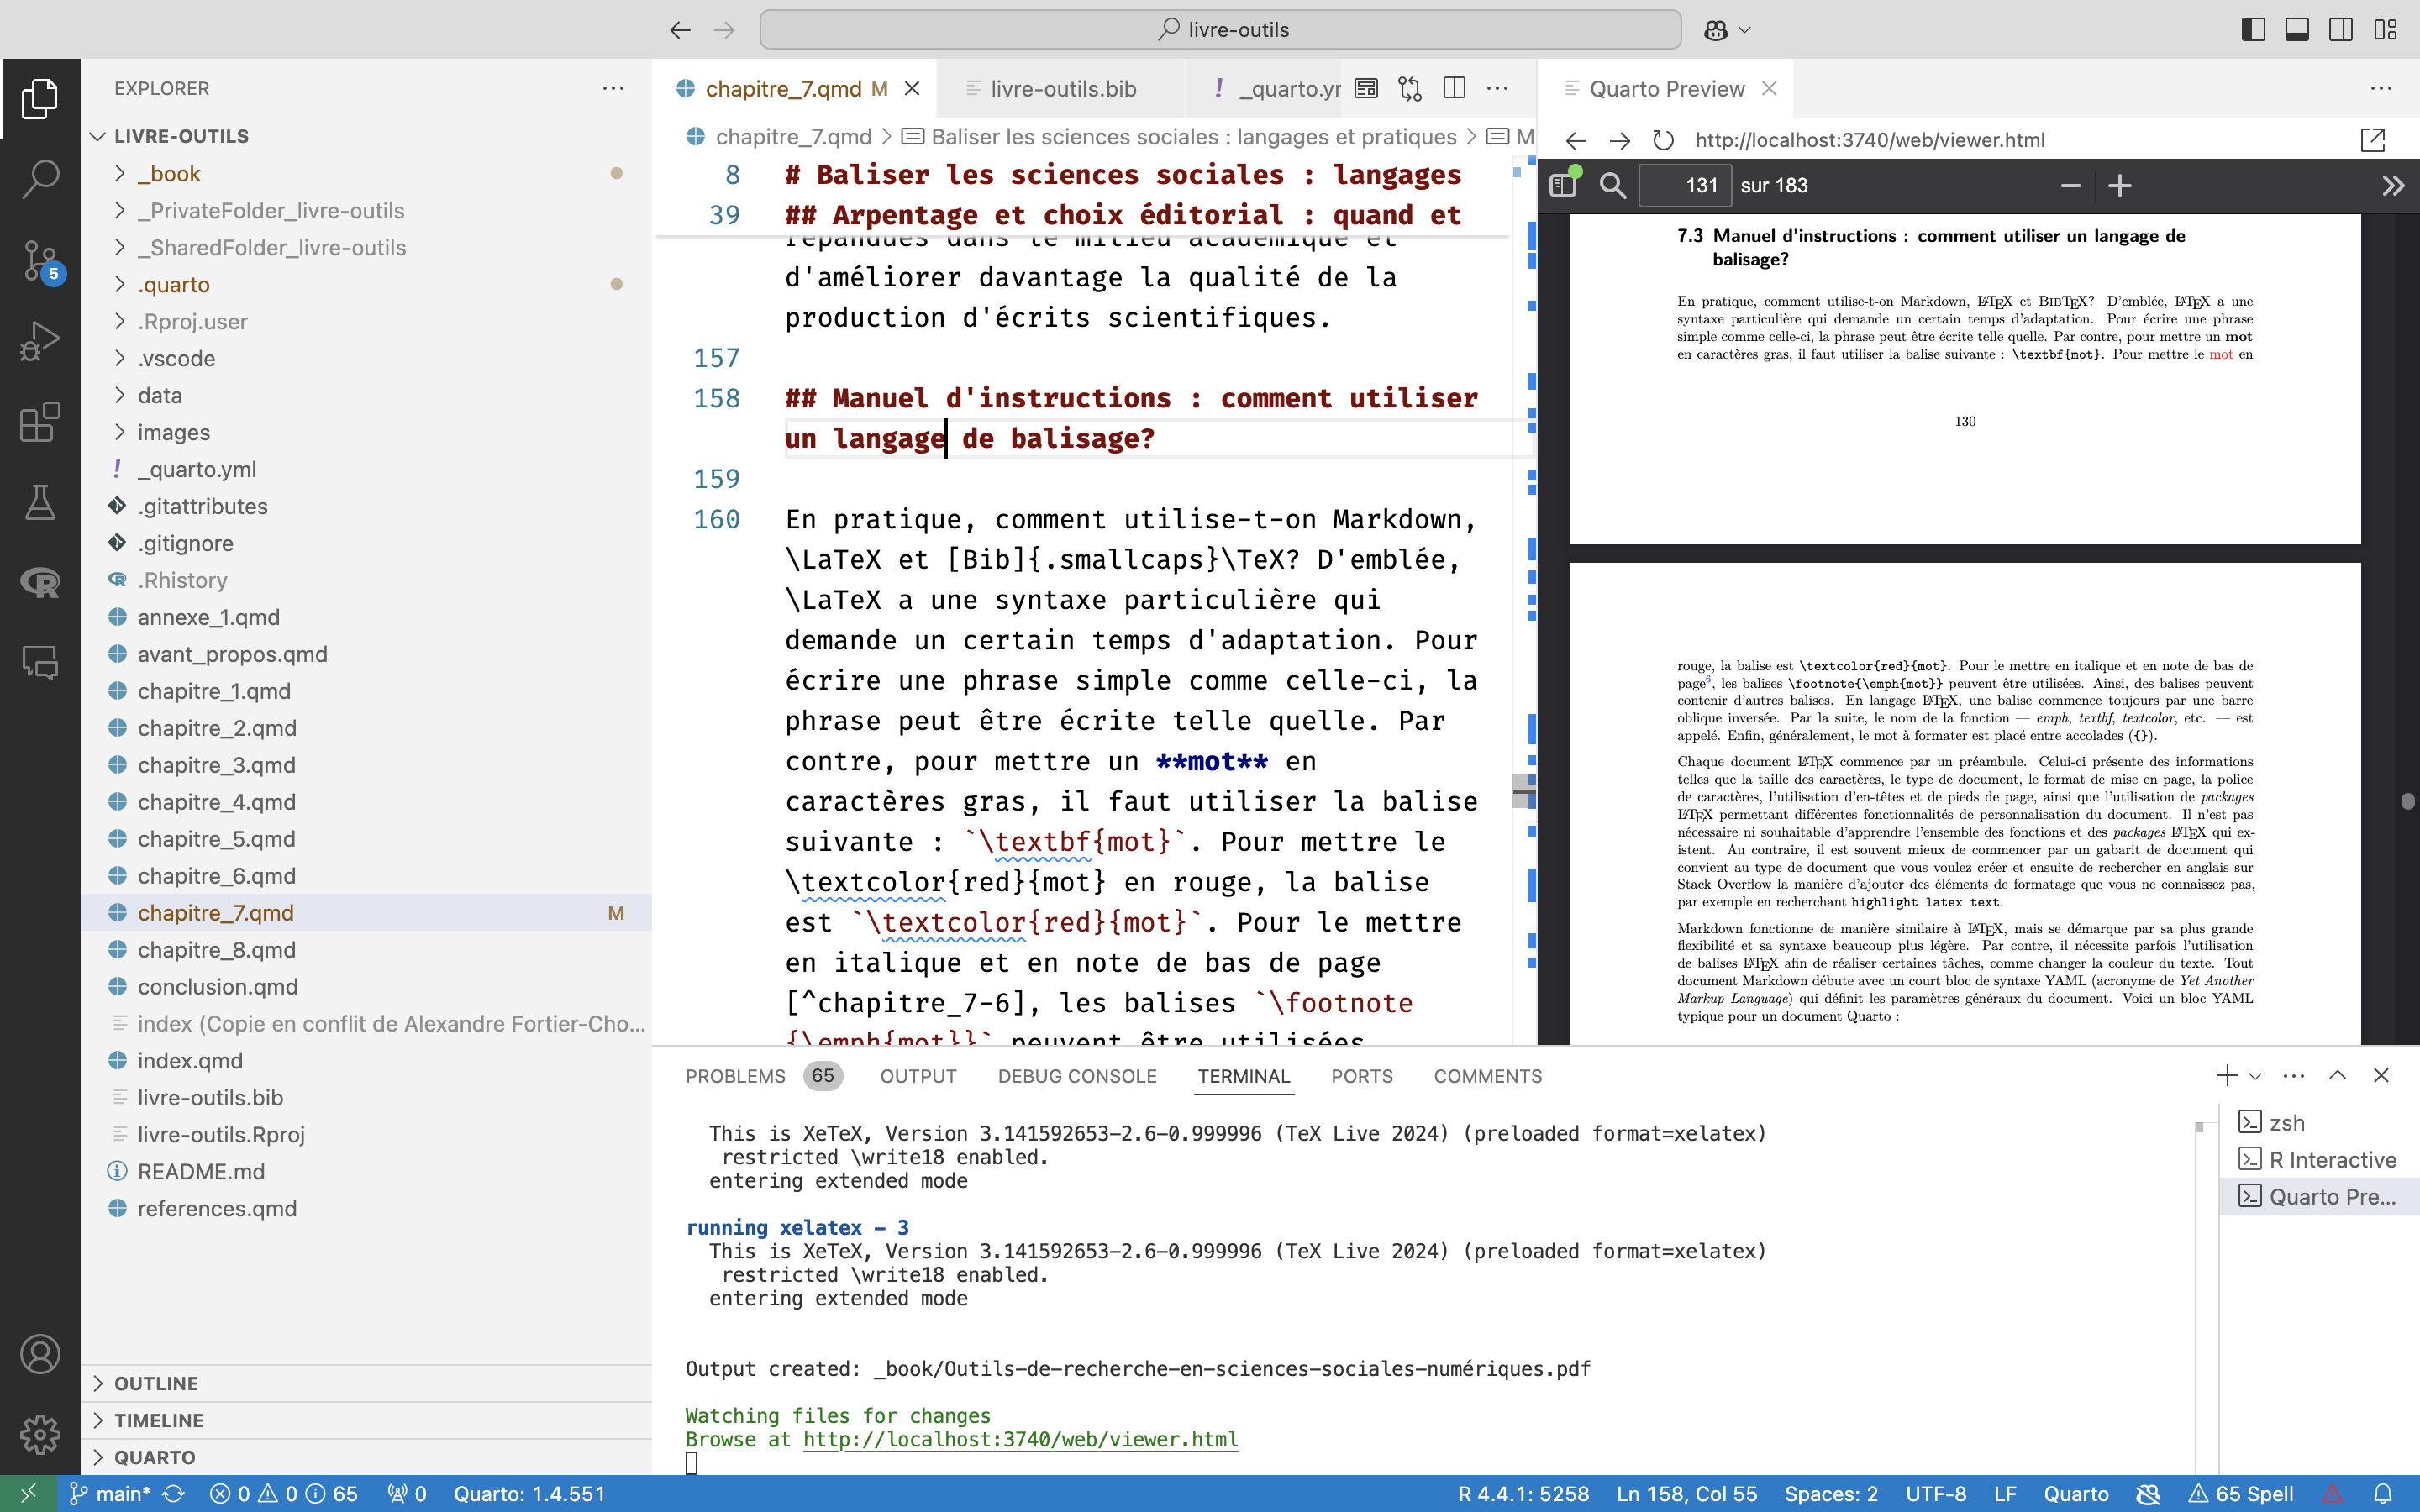
\includegraphics{images/chapitre7_vscode.png}

}

\caption{\label{fig-vscode}Exemple d'utilisation du langage de balisage
Markdown dans un fichier Quarto sur la plateforme VS Code
\newline \textit{Source}~: Auteurs du présent chapitre.}

\end{figure}%

Le premier langage de balisage, le Generalized Markup Language (GML), a
été inventé en 1969 par les chercheurs Charles F. Goldfarb, Ed Mosher et
Ray Lorie pour la compagnie IBM. Goldfarb et ses collègues devaient
intégrer trois applications créées avec des langages différents et avec
une logique différente pour les besoins d'un bureau de droit. Même après
avoir créé un programme qui permettait aux trois applications
d'interagir, ces langages demeuraient différents et avaient chacun leur
propre fonctionnement. Le développement de GML a permis de résoudre ce
problème en standardisant et en structurant le langage~: les mêmes
commandes étaient utilisées pour accomplir les mêmes tâches dans chaque
programme (Goldfarb, 1996). GML a été amélioré durant les décennies
suivantes et a été suivi par d'autres langages de balisage, dont
\LaTeX~en 1985, \textsc{Bib}\TeX~en 1988, HTML en 1993, XML en 1998,
Markdown en 2004 et \texttt{R} Markdown en 2012 (Encyclopaedia
Britannica, 2023; Hameed, 2023; Markdown Guide, 2023; World Wide Web
Consortium, 1998; Xie, 2023).

Les langages de balisage permettent d'effectuer différentes tâches.
HTML, qui est sans doute le plus connu des langages de balisage, permet
de formater des sites Web. XML, quant à lui, permet de structurer de
larges volumes de données. \LaTeX permet pour sa part de formater du
texte et de créer des documents en format PDF. Markdown permet également
de créer des documents en format PDF, mais aussi en format HTML ou DOCX
--- format utilisé pour les documents Word ---, contrairement à \LaTeX.
\texttt{R} Markdown permet aussi d'ajouter des extraits de code
\texttt{R} à un fichier en langage Markdown. Enfin, depuis 2022, le
système de publication scientifique et technique multilingue Quarto
permet de créer des documents qui intègrent des extraits de code
\texttt{R}, \LaTeX, Python, Julia ou JavaScript, créés dans différents
types d'environnements, à un fichier en langage Markdown (Allaire,
2022). \LaTeX, Markdown, \texttt{R} Markdown et Quarto permettent aussi
d'intégrer les références bibliographiques du système de traitement de
références \textsc{Bib}\TeX. Les langages de balisage communiquent ainsi
souvent les uns avec les autres au sein d'un même fichier. Le chapitre 4
explique la manière de citer les références en langage
\textsc{Bib}\TeX par le biais de Zotero et de Better \textsc{Bib}\TeX.

Pour mieux comprendre ces différents langages, il est utile de les
concevoir selon différents niveaux d'abstraction. L'abstraction, définie
comme le processus qui consiste à simplifier des systèmes complexes en
se concentrant sur les aspects essentiels (Hazzan, 2002; J. Kramer,
2007), constitue un concept fondamental en informatique. Dans le
contexte des langages de balisage, cette perspective permet de
distinguer différents niveaux selon leur complexité syntaxique et leur
facilité d'utilisation. Comme le souligne Neumanns (2019), il existe une
tension fondamentale entre la facilité d'usage et la puissance pour les
documents complexes. Bien que les langages de balisage forment en
réalité un continuum entre puissance et simplicité (Arloing et al.,
2016), ce chapitre propose de les organiser selon trois niveaux
d'abstraction pour faciliter leur compréhension. Cette simplification
pédagogique, illustrée dans la Figure~\ref{fig-niveaux-abstraction},
permet de distinguer les principales approches de balisage selon leur
complexité d'usage.

\begin{figure}

\centering{

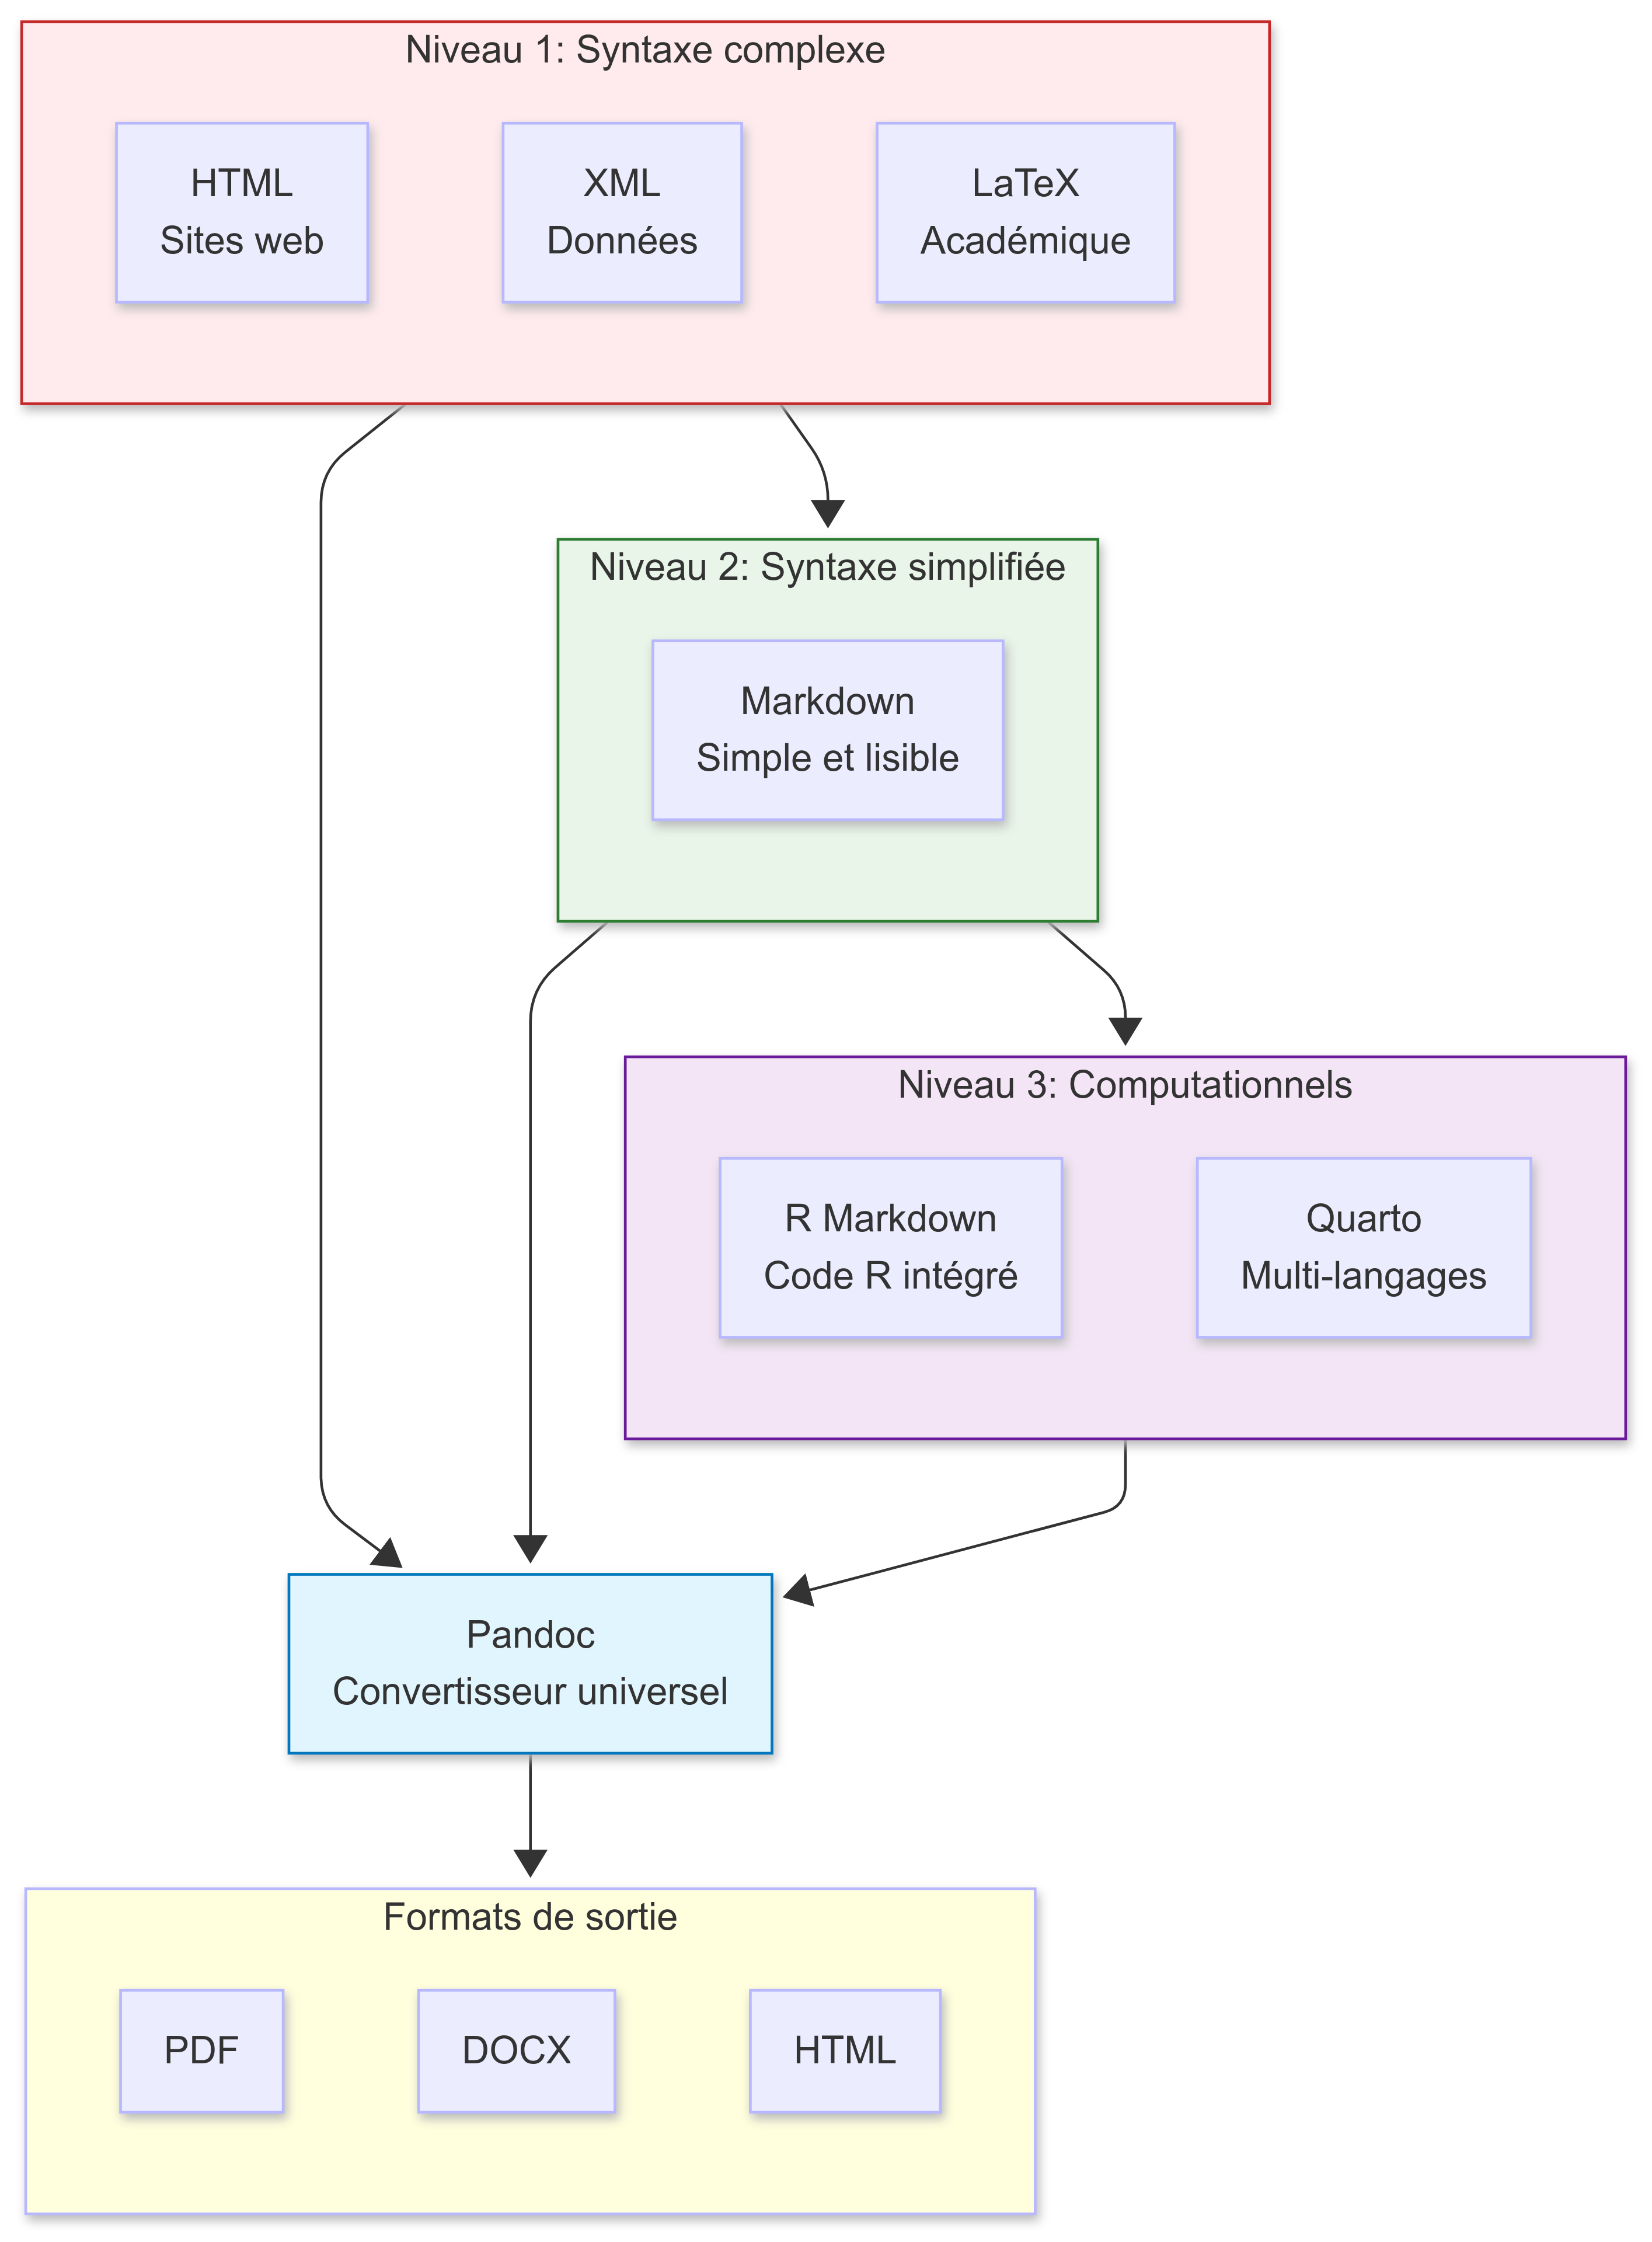
\includegraphics[width=0.9\textwidth,height=\textheight]{images/chapitre7_mermaid1.png}

}

\caption{\label{fig-niveaux-abstraction}Niveaux d'abstraction des
langages de balisage selon leur complexité syntaxique et leur
flexibilité d'usage \newline \textit{Source}~: Auteurs du présent
chapitre.}

\end{figure}%

Les langages à syntaxe complexe constituent le premier niveau de cette
hiérarchisation. Ces langages nécessitent de spécifier explicitement de
nombreux détails techniques (Grätzer, 2008). L'utilisateur doit
comprendre et contrôler directement les mécanismes sous-jacents :
balises détaillées en HTML, schémas complexes en XML, commandes
typographiques précises en \LaTeX. Au deuxième niveau, un langage comme
Markdown simplifie l'interaction en cachant la complexité technique
derrière une syntaxe intuitive (Arloing et al., 2016). L'utilisateur se
concentre sur le contenu plutôt que sur les détails de formatage, le
système gérant automatiquement la conversion vers différents formats.

Le troisième niveau comprend les systèmes de publication
computationnelle. Contrairement aux langages traditionnels qui peuvent
être étendus pour supporter l'exécution de code, R Markdown et Quarto
sont conçus dès le départ pour intégrer programmation lettrée et
recherche reproductible (Allaire, 2022; Knuth, 1984). Ces systèmes
masquent automatiquement la complexité du balisage, de l'exécution du
code et de la génération de résultats dans un flux de travail unifié. Au
cœur de cet écosystème se trouve Pandoc, présenté comme un convertisseur
universel de documents (\emph{Pandoc - Index}, s.~d.). Pandoc peut
convertir entre plus de nombreux formats différents grâce à son
architecture modulaire : il lit un document dans un format donné, le
convertit en représentation intermédiaire, puis l'écrit dans le format
de sortie désiré. Cette capacité de conversion universelle explique
pourquoi Quarto et R Markdown peuvent produire des documents PDF, DOCX
et HTML à partir d'une seule source Markdown. Cette hiérarchisation
illustre comment l'abstraction permet de gérer la complexité (J. Kramer,
2007) : chaque niveau supérieur simplifie l'usage tout en s'appuyant sur
les capacités techniques des niveaux inférieurs.

Les balises constituent une manière de donner manuellement des commandes
au logiciel utilisé. Par contraste, avec Microsoft Word, une panoplie de
boutons permettent de formater le texte. Les balises exercent les mêmes
fonctions de formatage pour les fichiers produits en \LaTeX~ou en
Markdown, mais doivent être ajoutées à l'écrit par l'utilisateur.
Lorsque l'on appuie sur un bouton pour formater le texte ou que l'on
utilise une commande comme \texttt{Ctrl-G} ou \texttt{Cmd-I} dans Word,
en réalité, cette commande ajoute des balises au travers du texte, mais
rend celles-ci invisibles dans l'interface utilisée. Cela permet d'avoir
un texte élégant et facile à lire, mais comporte aussi plusieurs
inconvénients. Le principal inconvénient est de limiter le pouvoir de
l'utilisateur sur le formatage de son texte. En effet, si les boutons à
sa disposition dans le logiciel de traitement de texte ne lui permettent
pas de réaliser une action, celle-ci sera éternellement impossible à
réaliser pour lui. A contrario, les langages de balisage permettent un
contrôle presque infini sur les opérations que l'on souhaite réaliser.
Incidemment, dans la mesure où l'on utilise le langage approprié pour la
tâche que l'on souhaite accomplir, il est possible de donner exactement
la commande nécessaire pour réaliser cette action. Bien que
l'utilisation de langages de balisage puisse paraître complexe à
première vue, il convient de rester attentif aux avantages qu'ils
procurent. Les langages de balisage, au-delà du coût d'apprentissage et
de l'interface de travail moins intuitive qu'un document Word, offrent
notamment une plus grande flexibilité.

Afin d'utiliser un langage de balisage, il est impératif que le logiciel
ou environnement de développement intégré utilisé puisse prendre en
compte ce langage. Un logiciel permet rarement d'utiliser n'importe quel
langage. Par exemple, le logiciel \TeX{}Shop permet seulement d'utiliser
le langage \LaTeX. Il est aussi important de bien utiliser le langage de
balisage. En effet, comme pour les langages de programmation, les
langages de balisage ne peuvent pas déduire ce que l'on souhaite leur
faire comprendre. Pour mettre du texte en gras, il faut utiliser les
bonnes balises. La moindre erreur peut être coûteuse, puisqu'une erreur
dans la balise utilisée risque de produire une commande incompréhensible
et un message d'erreur, le logiciel ne réussissant pas à associer la
balise mal inscrite à une action informatisée. Conséquemment, il est
impératif de bien vérifier les balises utilisées afin d'éviter toute
erreur qui empêcherait le document d'être compilé, c'est-à-dire d'être
traduit dans son format final\footnote{Certains logiciels et
  environnements de développement intégrés permettent d'identifier les
  balises problématiques plus facilement que d'autres. Certains ne
  produisent qu'un message d'erreur sans donner d'indication sur la
  source du problème, alors que d'autres ciblent très spécifiquement la
  ligne de syntaxe où se situe la balise problématique.}. Chaque
caractère dans une balise est important et il y a rarement plus d'une
seule manière de commander une action. Par exemple, en \LaTeX, il n'y a
qu'une seule manière de mettre du texte en gras. Il faut précisément
utiliser cette commande~: \texttt{\textbackslash{}textbf\{\}}. Le
positionnement des balises est lui aussi critique~: il délimite la
portion de texte à laquelle doit être appliquée l'action commandée par
la balise.

Dans le contexte de la recherche en sciences sociales, la programmation
est généralement utilisée afin de récolter, d'analyser et de présenter
visuellement des données. Une fois cartes, tableaux et graphiques
produits, ceux-ci peuvent être enregistrés --- par exemple en format PDF
ou PNG --- et inclus au sein d'un document qui sera formaté en utilisant
un langage de balisage. En \texttt{R} Markdown et en Quarto, des
extraits de langage de programmation peuvent être inclus dans des
sections bien délimitées de documents écrits en langage de balisage.
Plus généralement, le langage de programmation contribue à l'analyse
alors que le langage de balisage est essentiellement utile afin de
présenter les travaux de recherche, que ce soit dans un document écrit
ou sur un site Web. C'est principalement de cette manière que sont
utilisés les langages de programmation et de balisage dans le cadre de
la recherche en sciences sociales.

\section{Arpentage et choix éditorial~: quand et pourquoi utiliser un
langage de
balisage?}\label{arpentage-et-choix-uxe9ditorial-quand-et-pourquoi-utiliser-un-langage-de-balisage}

La plupart des langages de balisage permettent de remplir l'une des deux
fonctions suivantes, qui sont particulièrement importantes dans le
contexte de la recherche en sciences sociales~: produire des documents
écrits et formater des pages Web. Dans les deux cas, ces actions peuvent
être réalisées à partir de logiciels simples, mais ces logiciels ont des
limites importantes auxquelles les langages de balisage apportent des
solutions\footnote{Les langages de balisage permettent également de
  créer des pages Web. Bien que des plateformes comme WordPress
  facilitent cette tâche, HTML offre plus de personnalisation et
  d'automatisation. Il s'agit encore d'une question d'abstraction :
  WordPress simplifie l'usage en s'appuyant sur HTML et JavaScript.}.

Pour l'écriture de documents très simples comme une liste d'épicerie ou
des notes rapides pendant une conférence, les logiciels de traitement de
texte sont tout à fait convenables~: ils sont simples et rapides à
utiliser, un formatage professionnel du document n'est pas de mise.
Utiliser un langage de balisage pour des tâches de base peut en effet
rendre la tâche inutilement longue et complexe. Toutefois, plus la
complexité d'un document augmente, plus il devient difficile d'obtenir
un résultat satisfaisant en utilisant un logiciel de traitement de texte
tel que Word, Pages ou Writer. A contrario, \LaTeX~permet de produire
des documents de tous les niveaux de complexité, tel que démontré sur la
Figure~\ref{fig-latex-vs-word}. Quant à Markdown, sa courbe
d'apprentissage se situerait logiquement entre celles de \LaTeX~et de
Word, puisque ses balises sont simplifiées. Plus généralement, utiliser
un langage de balisage comme \LaTeX~ou Markdown\footnote{Les avantages
  et désavantages de Markdown cités dans cette section s'appliquent
  également à Quarto et à \texttt{R} Markdown, puisque ces derniers font
  appel au langage Markdown.} comporte plusieurs avantages par rapport
aux logiciels de traitement de texte traditionnels (voir le Tableau
7.1). Ces avantages font tous appel à un mélange de quatre concepts
principaux~: \emph{automatisation}, \emph{personnalisation},
\emph{flexibilité} et \emph{qualité graphique}.

\begin{figure}

\centering{

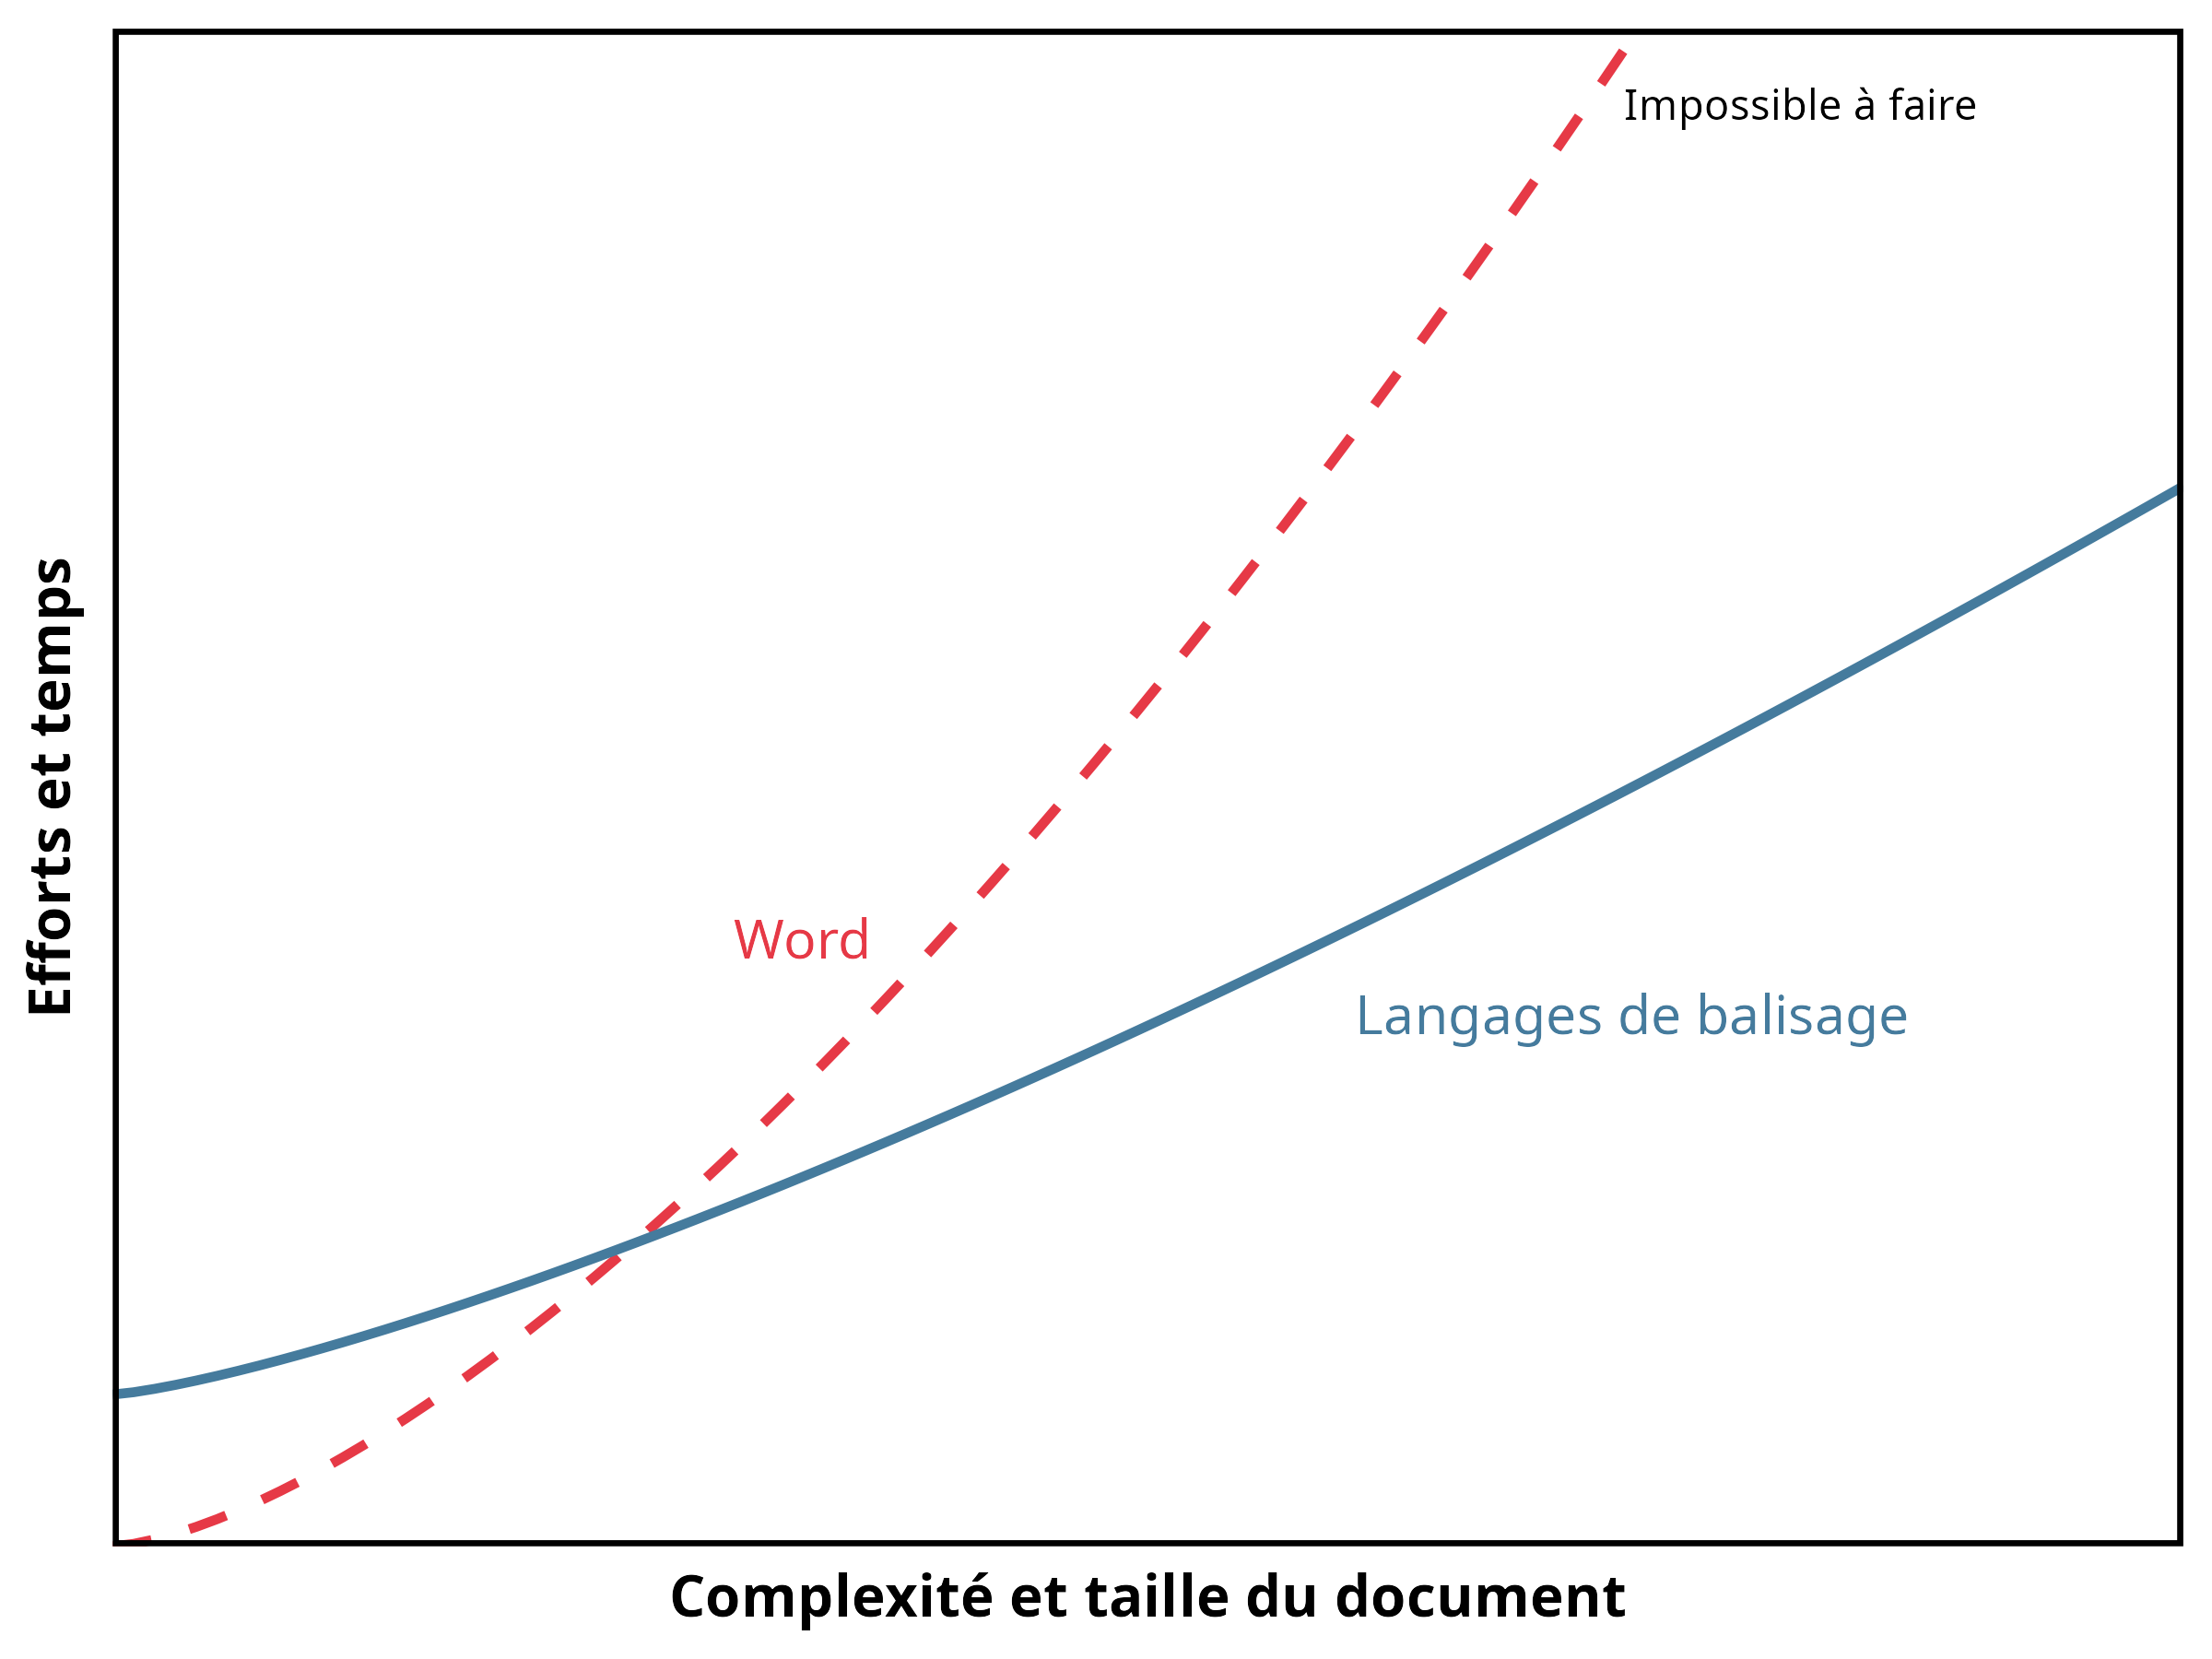
\includegraphics[width=0.7\textwidth,height=\textheight]{images/chapitre7_word-vs-latex.png}

}

\caption{\label{fig-latex-vs-word}Utilité relative de Word et des
langages de balisage selon la complexité et la taille du document
\newline \textit{Source}~: Auteurs du présent chapitre inspiré de Quang
Trung Luu (2023).}

\end{figure}%

\begin{table}
\centering
\begin{talltblr}[         %% tabularray outer open
caption={Tableau 7.1: Comparaison des outils de rédaction},
note{a}={Bien que \LaTeX\ offre une bonne transparence et réplicabilité, son utilisation via Overleaf peut être limitée sans version payante, notamment pour l'intégration avec GitHub et Dropbox. Ces limitations ne s'appliquent pas à des environnements comme RStudio ou VS Code.},
note{b}={Quarto est relativement récent et semble prendre de plus en plus la place de R Markdown parmi la communauté d'utilisateurs de R. Le nombre d'utilisateurs de Quarto est donc appelé à croître dans les prochaines années.},
]                     %% tabularray outer close
{                     %% tabularray inner open
width={0.95\linewidth},
colspec={X[0.35]X[0.15]X[0.15]X[0.15]X[0.15]},
}                     %% tabularray inner close
\toprule
Critères & LaTeX & R Markdown & Quarto & Word \\ \midrule %% TinyTableHeader
Accessibilité (Gratuit ou peu dispendieux) & Oui & Oui & Oui & Non \\
Existence d'une communauté d'utilisateurs & Très grande & Grande & Moyenne\textsuperscript{b} & Très grande \\
Popularité dans le champ & Oui & Oui & Oui & Oui \\
Compatibilité avec d'autres outils & Moyenne & Forte & Forte & Faible \\
Transparence et réplicabilité & Oui\textsuperscript{a} & Oui & Oui & Non \\
Adaptabilité et flexibilité & Très forte & Forte & Forte & Forte \\
\bottomrule
\end{talltblr}
\end{table}

\subsection{Avantages}\label{avantages}

\subsubsection{Référencement}\label{ruxe9fuxe9rencement}

Premièrement, \LaTeX~et Markdown permettent d'intégrer une bibliographie
\emph{automatique} et professionnelle en utilisant \textsc{Bib}\TeX.
Cette bibliographie peut être adaptée très facilement en différents
styles bibliographiques reconnus ou en un style bibliographique
\emph{personnalisé} à partir d'un des nombreux gabarits professionnels
disponibles. Avec \textsc{Bib}\TeX, il n'y a pas à vérifier si le titre
de l'article est toujours en italique, si le numéro de volume est
toujours entre parenthèses ou si le nom de famille des deuxièmes auteurs
est toujours avant ou après le prénom puisque toutes ces opérations sont
effectuées de manière \emph{automatique}. \textsc{Bib}\TeX~comprend
également les différences entre les types de sources --- articles
scientifiques, livres, sites Internet, etc. --- et ajuste leur
présentation en conséquence. De plus, si l'une des sources citées n'est
pas incluse dans la bibliographie, une erreur s'affiche, permettant
d'identifier le problème plutôt que de se retrouver avec une référence
manquante. À l'inverse, si une source est retirée du texte, elle
disparait \emph{automatiquement} de la bibliographie dans le document
final mais demeure présente dans le fichier où se trouvent les
références bibliographiques. Cela évite les aller-retour pour vérifier
que chaque source de la bibliographie se trouve au moins une fois dans
le texte et que chaque source dans le texte est citée en bibliographie.
Grâce aux balises, en cliquant sur les références incluses dans le
document, on se retrouve immédiatement plus loin dans le document, à
l'endroit où se trouve l'entrée bibliographique associée. Les références
\textsc{Bib}\TeX~pour articles scientifiques peuvent généralement être
copiées-collées à partir de Google Scholar, en cliquant en dessous d'une
source sur «~Citer~» puis «~BibTeX~». \textsc{Bib}\TeX~rend donc
extrêmement simple et efficace l'utilisation des références
bibliographiques grâce à sa capacité à \emph{personnaliser} et
\emph{automatiser} leur présentation\footnote{L'utilisation d'un
  logiciel de traitement de texte, en particulier lorsque combiné avec
  une extension Zotero, peut également produire un résultat automatisé
  et personnalisé à un certain degré. Cependant, au moment où ce
  chapitre est écrit, le retrait d'une citation du texte principal en
  Word avec Zotero n'enlève pas immédiatement cette citation de la
  bibliographie, et l'ajout de liens vers la bibliographie doit se faire
  source par source, ce qui prend un temps important et peut occasionner
  des erreurs humaines. Ainsi, les logiciels de traitement de texte
  peuvent devenir contraignants lorsqu'un utilisateur cherche à
  accomplir une tâche qui ne cadre pas avec leurs fonctionnalités de
  base. Dans ces cas, les langages de balisage plus complexes et donc de
  plus bas niveau d'abstraction peuvent offrir plus de contrôle à
  l'utilisateur.}.

\subsubsection{Figures et tableaux}\label{figures-et-tableaux}

L'intégration de figures et de tableaux dans le texte est aussi rendue
très simple et professionnelle grâce à \LaTeX~et à Markdown. La taille
de la figure ou du tableau, son positionnement et son intégration par
rapport au texte environnant peuvent être réglés avec précision.
Cependant, l'ajout de texte avant ou après la figure ou le tableau ne
produira pas des résultats inattendus tels qu'une demi-page vide avant
un graphique ou un titre de tableau complètement en bas d'une page. En
définissant des paramètres pour l'ensemble du texte, le chercheur peut
\emph{personnaliser} entièrement la présentation des figures et des
tableaux. De plus, la \emph{qualité des figures et des tableaux} ne
diminue pas lors de leur intégration~: les figures restent aussi belles
qu'elles l'étaient originalement, ce qui n'est pas toujours le cas dans
les logiciels de traitement de texte. Les figures et les tableaux sont
aussi numérotés \emph{automatiquement}, ce qui veut dire que
l'utilisateur n'a jamais à se préoccuper de modifier les numéros si
l'ordre des figures et tableaux est modifié dans le texte. Grâce aux
balises, en cliquant sur le numéro associé à la figure ou au tableau
dans le texte, le document se retrouve automatiquement à l'endroit où se
trouve la figure ou le tableau. De plus, les figures peuvent être
intégrées en format PDF, ce qui permet au lecteur de sélectionner le
texte se trouvant sur le graphique directement, incluant les titres des
axes et les annotations, ce qui n'est pas possible avec les images PNG
intégrées dans Word ou autres logiciels similaires.

Surtout, l'intégration de graphiques produits par \texttt{R} au texte en
langage de balisage est simplifiée et \emph{automatisée}. En effet, même
lorsque les données ou le code pour produire un graphique changent,
\texttt{R} resauvegarde le fichier dans le même chemin d'arborescence
(\emph{path}) particulier que l'on a indiqué, par exemple
\texttt{C:/Users/Jean/Dropbox/projet1/graphs/Figure1.pdf}. Le langage de
balisage peut ensuite indiquer le même chemin d'arborescence, de sorte
qu'il n'est pas nécessaire de recopier-coller la figure à l'intérieur du
document chaque fois que des changements y sont apportés; la figure est
mise à jour \emph{automatiquement}. En plus, les figures et tableaux qui
sont ajoutés peuvent être automatiquement ajoutés à une liste de
tableaux et à une liste de figures juste après la table des matières,
dans le cas d'une thèse par exemple.

L'intégration de figures et de tableaux est particulièrement simple et
\emph{flexible} avec Quarto. Contrairement à \LaTeX, qui nécessite la
production de tableaux et de figures dans un document en langage de
programmation (comme \texttt{R}), Quarto permet de créer une figure
grâce à du code \texttt{R} \emph{et} d'intégrer celle-ci au texte dans
un même document. Cela se fait grâce à l'intégration de blocs de code
\texttt{R} (\emph{code chunks}) dans le document. Le code est produit
dans le bloc de code et la figure ou le tableau qui en résulte apparait
à la fois dans le document Quarto, où des balises supplémentaires
permettent d'adapter le formatage, et sur le document fini. Cependant,
certains \emph{packages} R tels que \emph{modelsummary} et
\emph{stargazer} permettent de créer des tableaux de régression de
grande qualité en format \LaTeX~(Arel-Bundock, 2022;
\textbf{hlavac22?}). Les tableaux de régression en format Markdown sont
pour l'instant plus difficiles à produire au-delà d'un certain niveau de
complexité, en raison des limitations du langage Markdown. Cela dit, il
est facile de produire des tableaux de très grande qualité en langage
\LaTeX~dans un fichier Markdown ou Quarto.

\subsubsection{Équations}\label{uxe9quations}

\LaTeX~permet également d'ajouter des équations mathématiques poussées
pour les projets de recherche qui les nécessitent. En effet, il existe
des balises pour chaque symbole mathématique, et celles-ci peuvent être
agencées de manière à former des équations cohérentes. Ces équations
peuvent être intégrées au sein même d'une phrase ou être mises de
l'avant dans un paragraphe à part centré. Voici un exemple d'équation
pour une régression multiple écrite en \LaTeX~:

\begin{equation}
    Y = \beta_0 + \beta_1 X_1 + \beta_2 X_2 + \beta_3 X_3 + \cdots + \beta_k X_k + \epsilon
\end{equation}

\subsubsection{Table des matières et mise en
page}\label{table-des-matiuxe8res-et-mise-en-page}

Markdown et \LaTeX~permettent aussi la gestion \emph{automatisée} de la
table des matières, et les références aux pages appropriées à partir de
la table des matières se mettent à jour en continu. La table des
matières prend en compte l'architecture du texte choisie manuellement
par le chercheur, qui est définie par des balises définissant différents
niveaux hiérarchiques de sections, sous-sections ou chapitres. Des
manières \emph{automatiques} de référencer les figures et les tableaux
dans des sections distinctes de la table des matières sont également
offertes, encore une fois \emph{personnalisables} au goût du chercheur.

Bien que la mise en page de documents produits via Markdown et
\LaTeX~puisse être définie entièrement manuellement par les personnes
plus expérimentées, les novices apprécieront les nombreux gabarits
(\emph{templates}) qui permettent de gérer \emph{automatiquement} la
mise en page clés en main. Les gabarits permettent de rendre l'apparence
d'un document plus esthétique et uniforme et peuvent être utilisés tels
quels ou servir de point de départ pour un chercheur souhaitant y
apporter certaines modifications sans toutefois partir d'une feuille
blanche. La majorité des personnes qui utilisent ces langages, même les
plus expérimentées, utilisent ces gabarits comme base lorsqu'elles
rédigent un document. Ces gabarits constituent une mine d'or puisqu'ils
rendent accessible le code Markdown ou \LaTeX~ayant servi à la
conception du gabarit, permettant au chercheur de comprendre comment est
obtenu le résultat que lui offre le gabarit. Incidemment, il est
possible d'identifier les sections de code produisant certains éléments
de mise en page --- positionnement des numéros de page, positionnement
du nom des auteurs en début de document, etc. --- et les modifier ou
s'en inspirer afin de modifier d'autres gabarits. L'utilisation de ces
gabarits peut s'avérer complexe au départ, mais retravailler ces
gabarits peut permettre de devenir autonome et de produire exactement le
résultat désiré en termes de mise en page, et surtout de les réutiliser.
En comparaison, les logiciels de traitement de texte rendent souvent
très ardue la mise en page uniforme d'un document, puisque cet élément
ne peut pas être \emph{automatisé}. La liste des gabarits disponibles
est extrêmement large, et ceux-ci ont une variété de fonctions. En
effet, une variété de gabarits professionnels et de haute \emph{qualité
graphique} sont offerts gratuitement en ligne pour des articles, des
livres, des rapports, des \emph{curriculum vitæs} (Figure~\ref{fig-cv})
ou encore des factures professionnelles (Figure~\ref{fig-invoice}).

\begin{figure}

\centering{

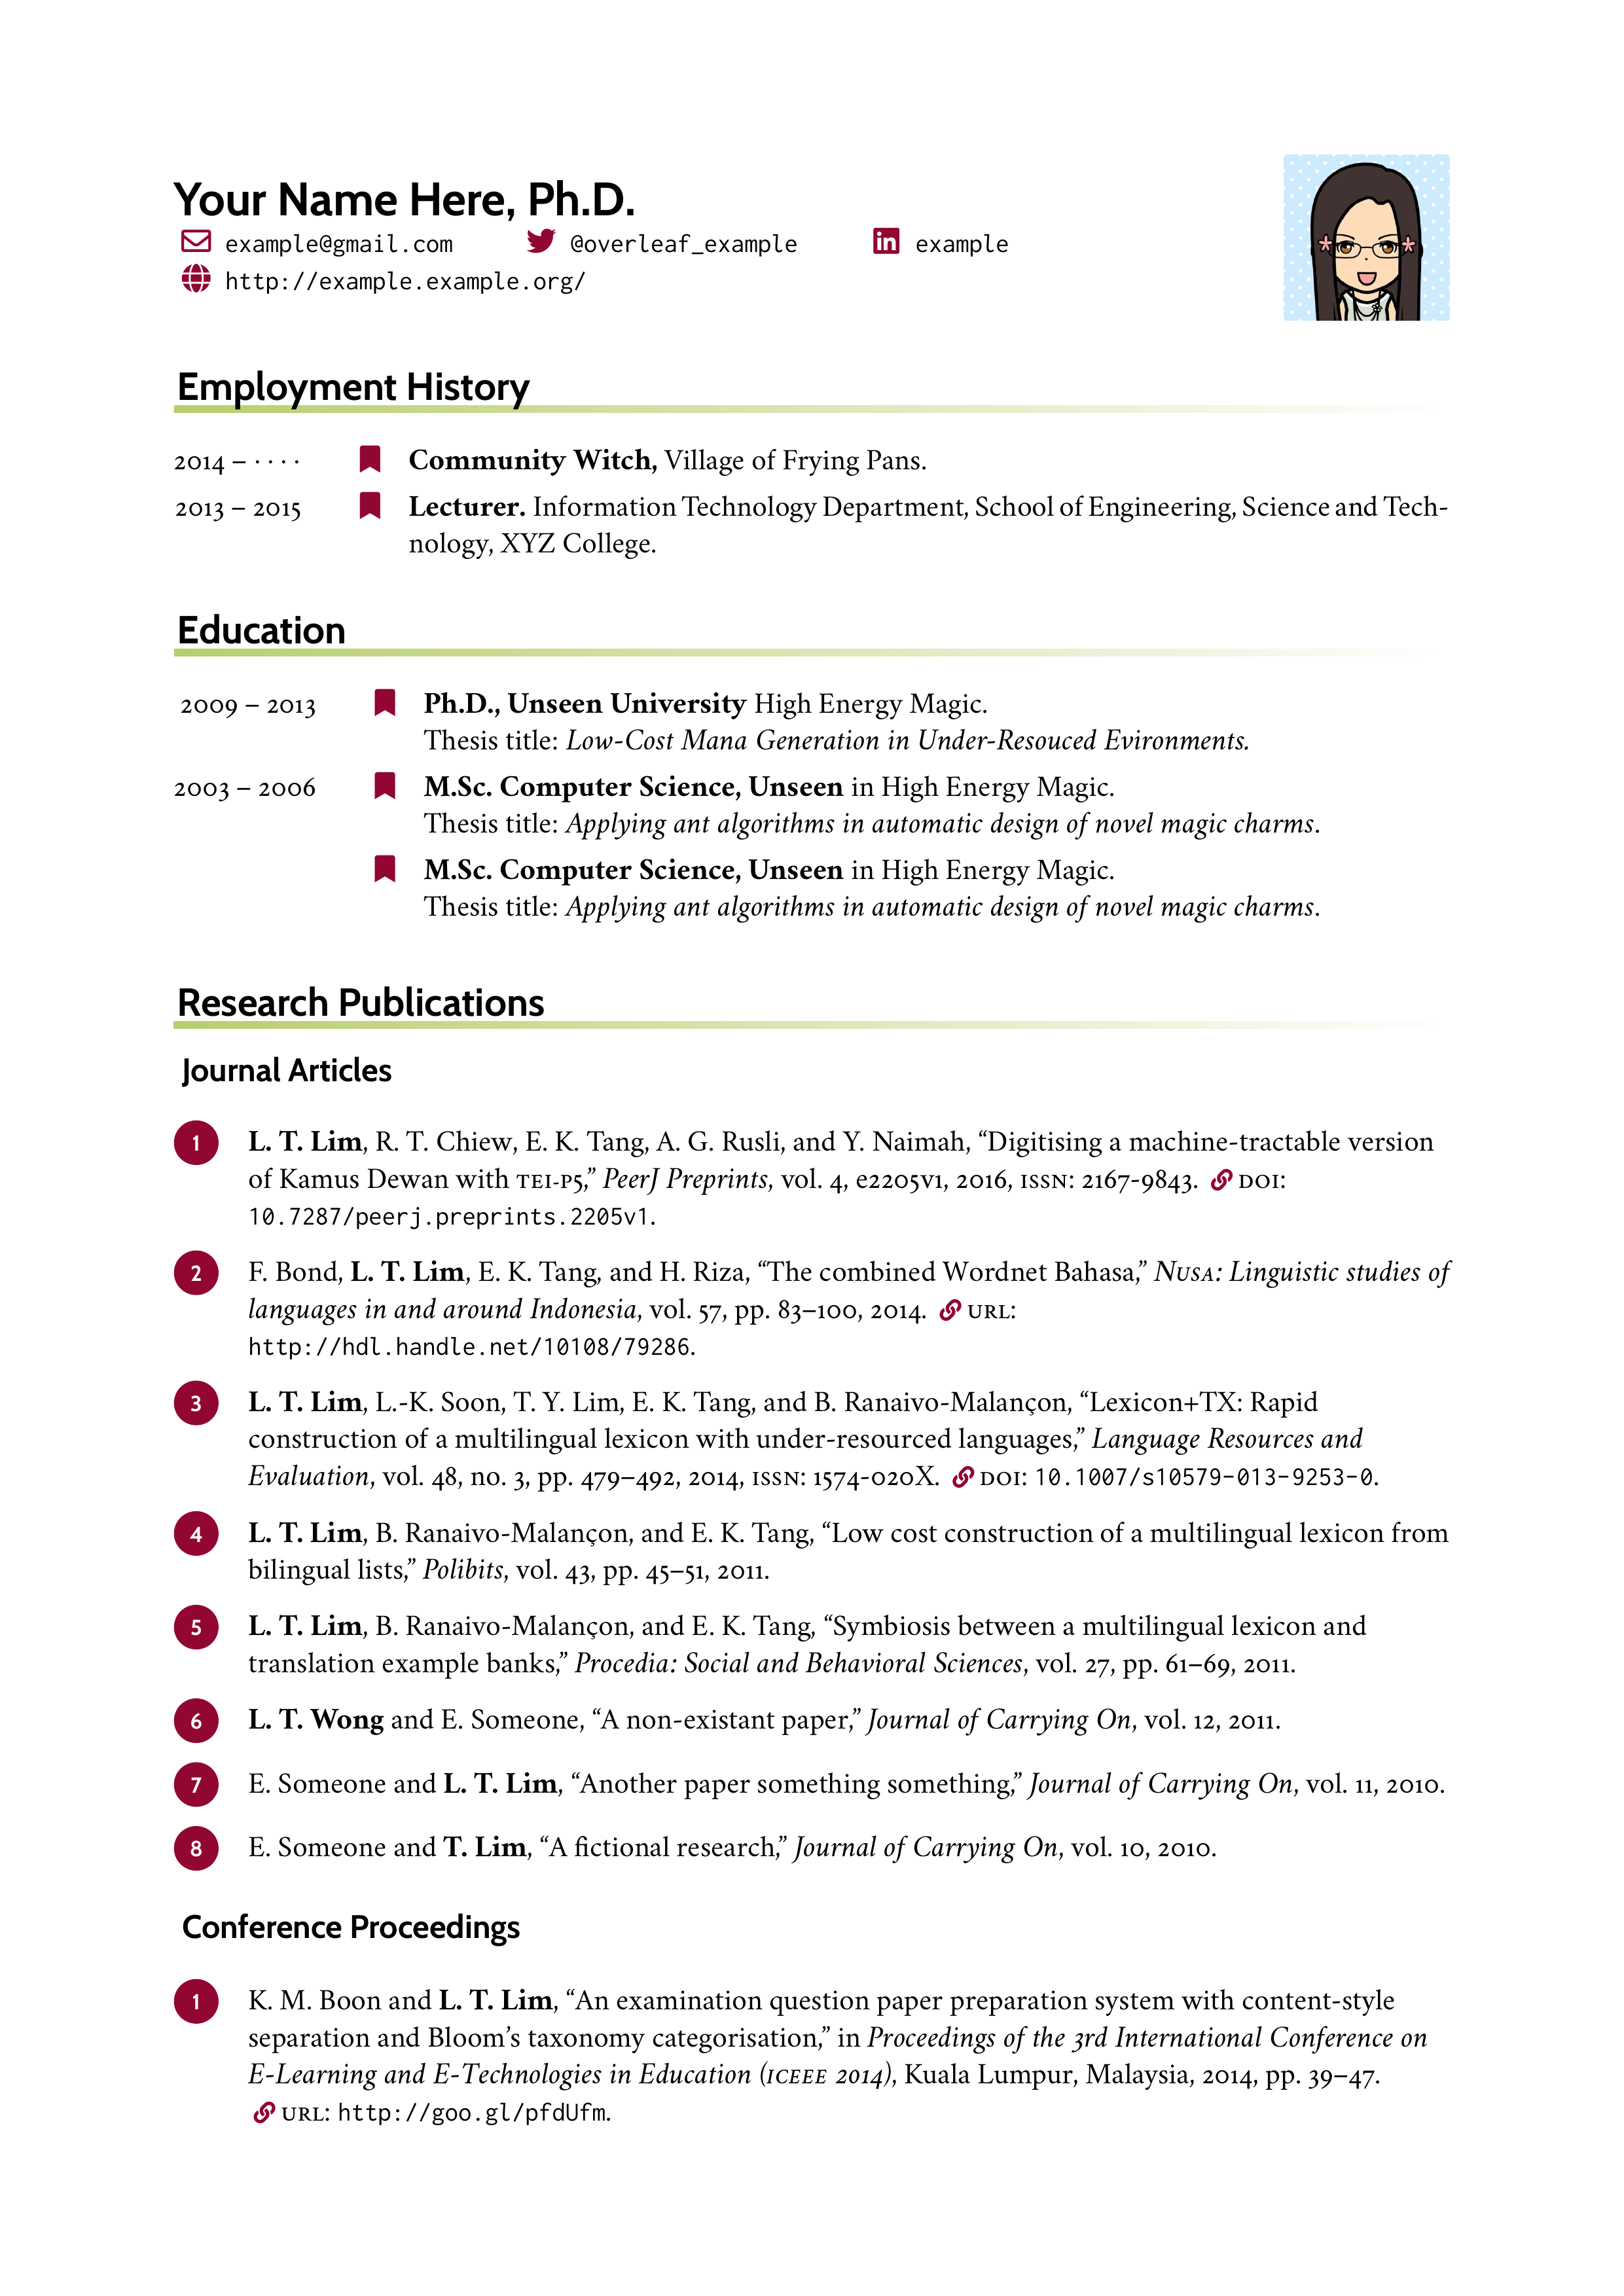
\includegraphics{images/chapitre7_CVtemp.png}

}

\caption{\label{fig-cv}Exemple de gabarit \LaTeX~de curriculum vitae
\newline \textit{Source}~: LianTze (2023).}

\end{figure}%

\begin{figure}

\centering{

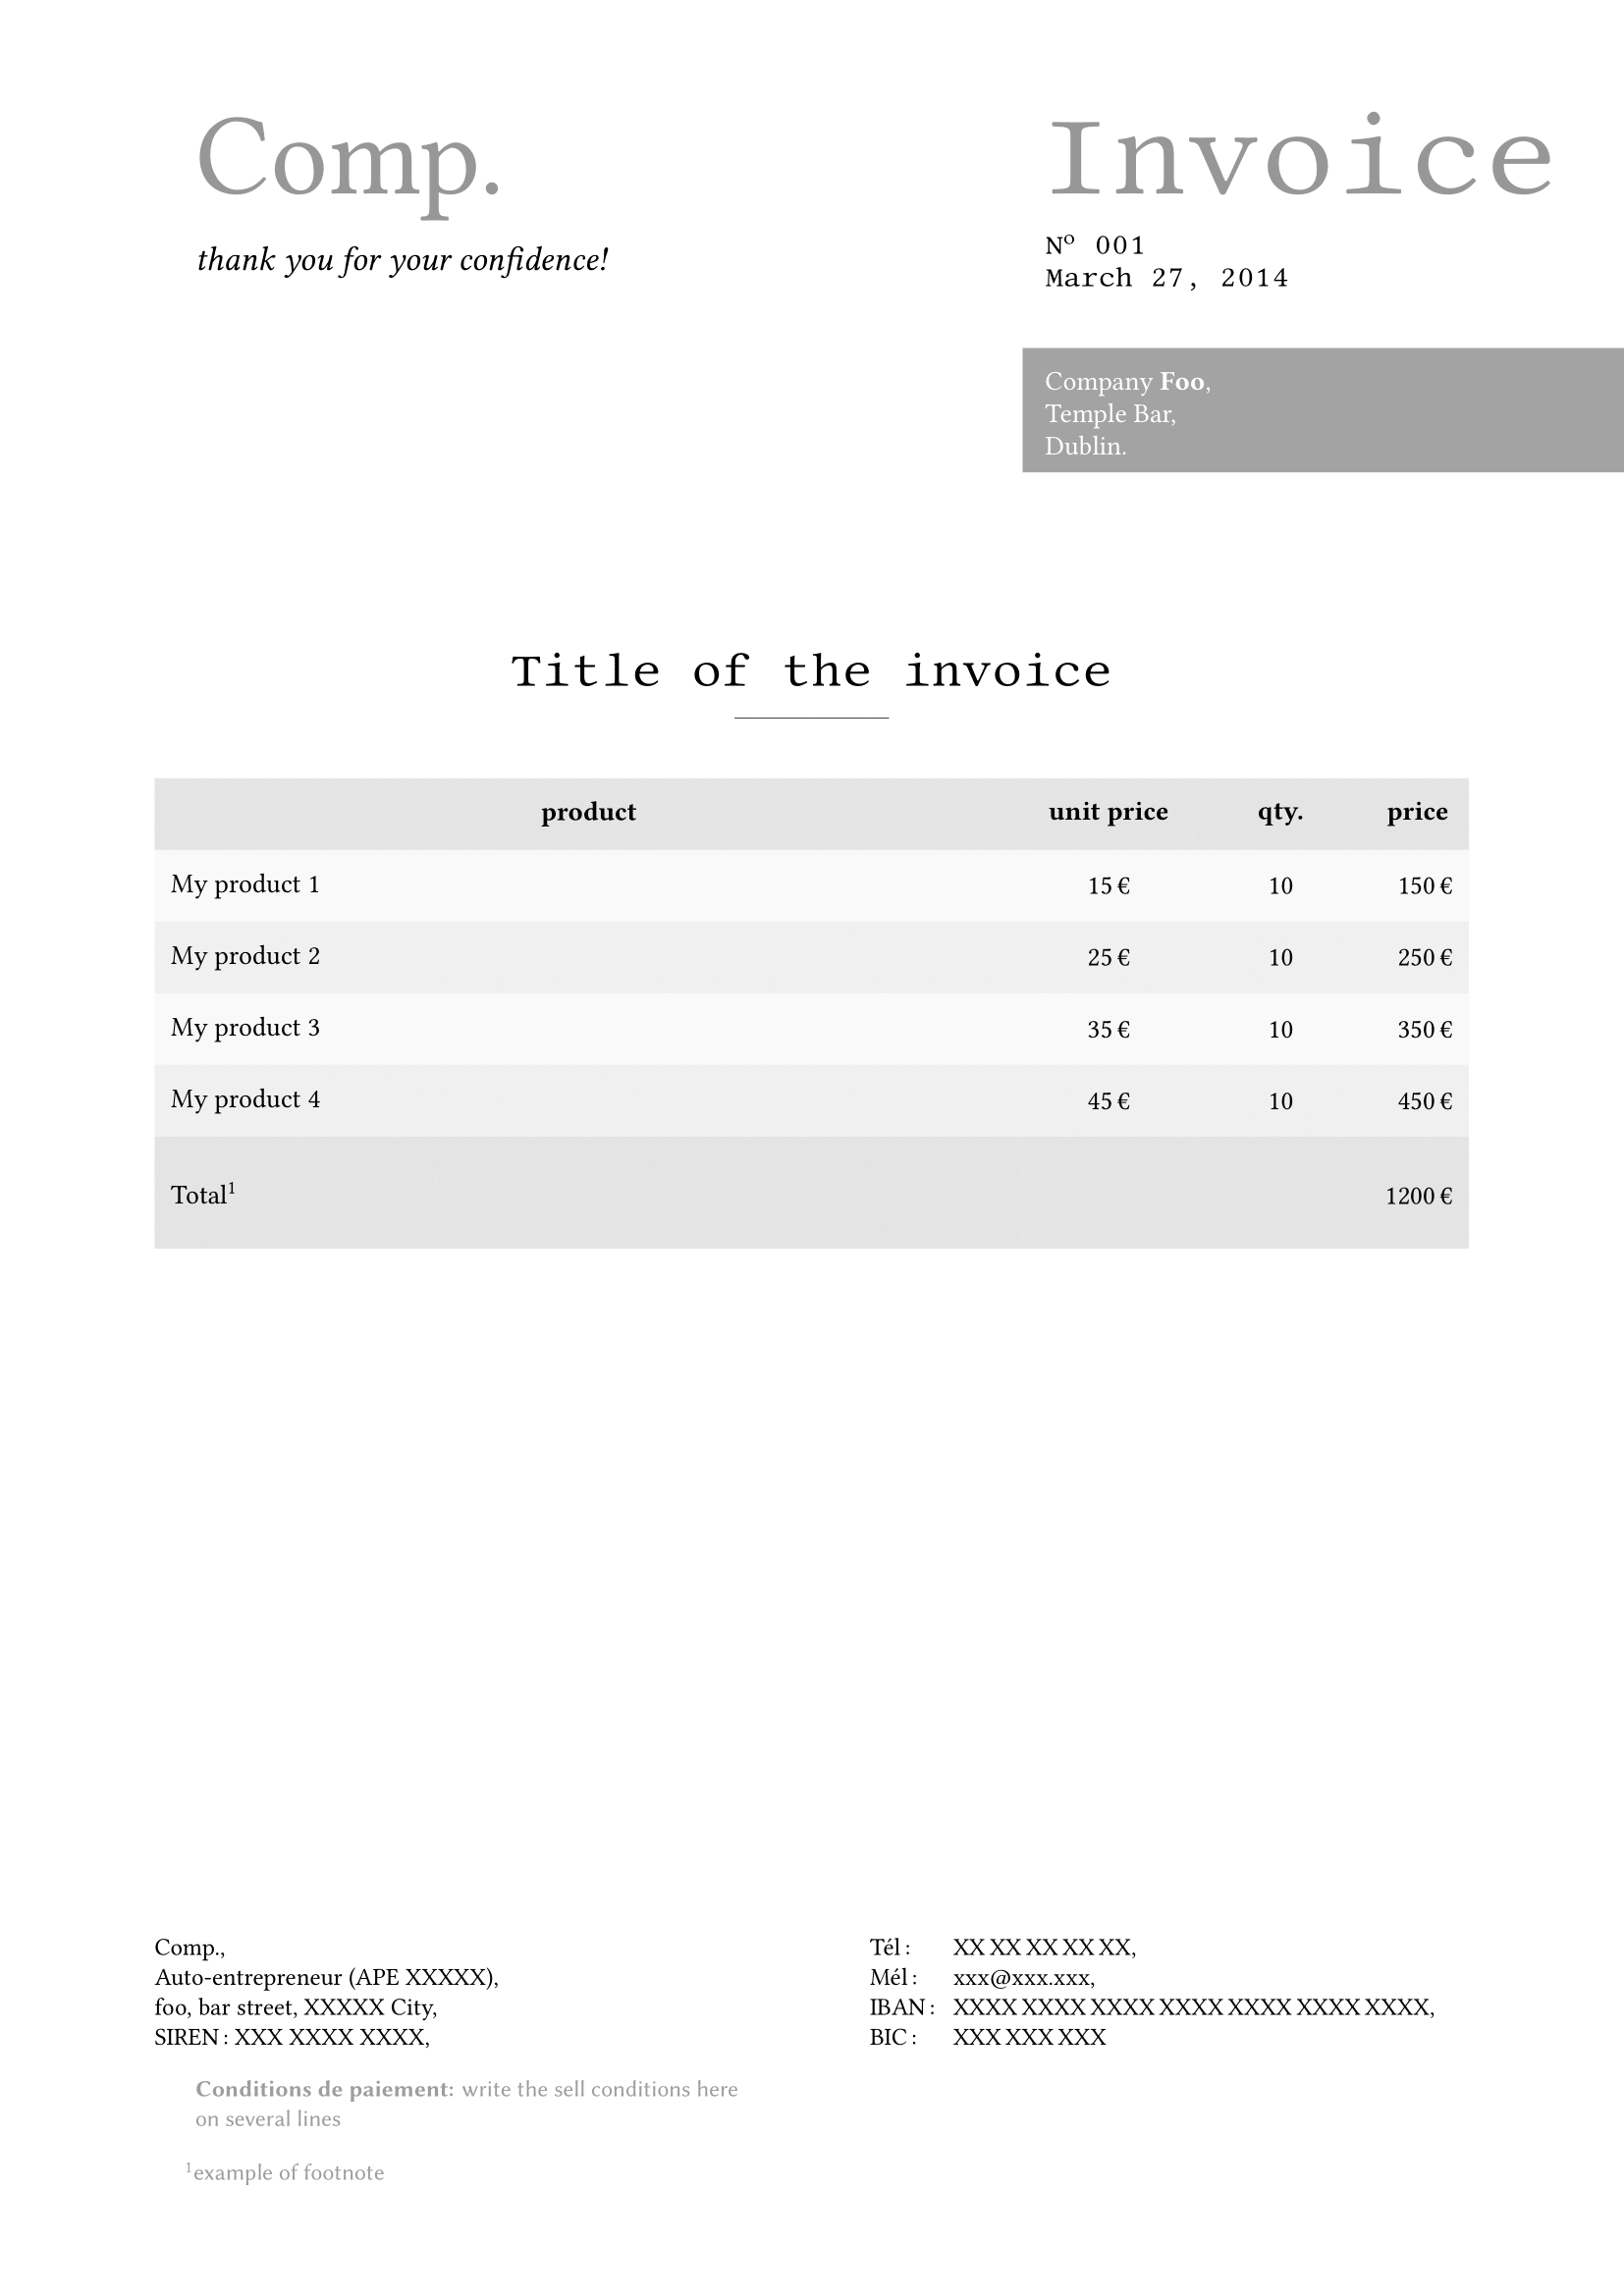
\includegraphics{images/chapitre7_TStemp.png}

}

\caption{\label{fig-invoice}Exemple de gabarit \LaTeX~de facture
\newline \textit{Source}~: Roux (2013).}

\end{figure}%

La Figure~\ref{fig-cv} et la Figure~\ref{fig-invoice} ne sont que
quelques exemples des milliers de gabarits de documents
\LaTeX~disponible en ligne. Plusieurs d'entre eux peuvent être
téléchargés à partir du site Web d'Overleaf (2023). Les utilisateurs
peuvent y naviguer et voir quel gabarit convient le mieux à leurs
besoins. Certaines manières plutôt spécifiques de formater le texte sont
présentement disponibles avec \LaTeX~ou Markdown bien que non
disponibles en Word, ce qui constitue une autre démonstration de leur
grande \emph{flexibilité} et capacité de \emph{personnalisation}. Bien
qu'il soit rare que l'on ait absolument besoin de personnaliser le texte
ainsi, ces possibilités peuvent s'avérer utiles lorsque l'on rédige un
texte qui doit se conformer en tout point à un gabarit spécifique. En
effet, certaines revues scientifiques, maisons d'édition et universités,
dans le cadre de la rédaction d'articles, de mémoires et de thèses par
exemple, imposent ce type de gabarit inflexible et parfois plutôt
capricieux.

\subsubsection{Compatibilité entre types de
documents}\label{compatibilituxe9-entre-types-de-documents}

Un autre avantage non négligeable de Markdown --- qui le distingue à cet
égard de \LaTeX~--- est la \emph{flexibilité} des formats de documents
qui peuvent être produits. En effet, Pandoc Markdown, une extension du
langage Markdown de base, permet d'intégrer dans un seul document
plusieurs langages de balisage différents tels que Markdown, \LaTeX~et
HTML. Quarto utilise Pandoc Markdown et est également habilité à
travailler avec des extraits de code \texttt{R} ou Python. Ceci permet
donc à l'utilisateur ou à l'utilisatrice de bénéficier des
fonctionnalités de différents langages dans un seul document, rendant
ainsi possible une variété de \emph{personnalisations} qui ne seraient
pas possibles autrement. Qui plus est, puisque Markdown permet de créer
des fichiers Word réguliers, PDF professionnels et HTML à partir d'un
même document, l'utilisateur peut choisir à sa convenance et à tout
moment de quelle manière sera compilé le document rédigé. Cette
possibilité de créer des documents Word est particulièrement pratique
dans le cadre de collaboration avec des chercheurs n'utilisant pas les
langages de balisage ainsi que lors de l'envoi de manuscrits à des
revues scientifiques, puisque certaines d'entre elles exigent de
recevoir ceux-ci sous forme de document Word.

\subsubsection{Popularité}\label{popularituxe9}

La popularité de certains langages de balisage dans le monde de la
recherche confère un avantage considérable à ceux qui savent les
utiliser. La maîtrise de ces langages offre aux chercheurs une
polyvalence lorsqu'ils doivent collaborer avec diverses équipes de
recherche utilisant différentes méthodes de travail. Par exemple, depuis
sa création, \LaTeX~a été adopté largement par le milieu de la
publication de travaux scientifiques (Gaudeul, 2007). À titre indicatif,
Overleaf, l'éditeur en ligne mentionné précédemment, était utilisé en
2022 par 11 millions d'utilisateurs et utilisatrices dans 189 pays
autour du globe. Plus de 2000 compagnies et 6800 universités utilisent
Overleaf pour écrire en \LaTeX~(Overleaf, 2024). La popularité des
langages de balisage en fait donc des outils utiles pour une personne
qui voudrait poursuivre une carrière en recherche académique.

\subsubsection{Gestion des embûches}\label{gestion-des-embuxfbches}

Bien que l'apprentissage de \LaTeX~et de Markdown puisse être parsemé de
nombreuses embûches, ces deux langages bénéficient d'une communauté
d'utilisateurs en ligne sur laquelle il est possible de s'appuyer afin
de résoudre tout problème rencontré, vu la popularité de ces langages.
Ces individus --- particulièrement les plus expérimentés --- sont
nombreux à partager leur expérience à leurs collègues rencontrant des
problèmes afin de contribuer à régler ceux-ci. Cette communauté est
présente sur une multitude de sites Web, bien que le point de rencontre
principal soit le forum Stack Overflow (2023), qui est également utilisé
pour régler des problèmes de programmation. Une simple recherche sur
Google d'un problème rencontré avec \LaTeX~ou Markdown offrira des liens
vers des échanges pertinents ayant eu lieu sur Stack Overflow ou encore
vers de la documentation technique. L'utilisateur peut donc filtrer les
résultats et observer les nombreuses solutions envisageables à son
problème afin de définir laquelle est la plus appropriée dans sa
situation. Il est important de noter, toutefois, que cette communauté
est nettement plus développée pour les utilisateurs de \LaTeX~que de
Markdown, puisque ce dernier langage est moins répandu que le premier.

Également, avec l'émergence de l'intelligence artificielle (IA), de
nombreux modèles d'IA génératifs commencent à émerger comme des
ressources d'aides utiles pour les chercheurs. Au moment de la rédaction
du présent chapitre, le \emph{chatbot} ChatGPT, développé par OpenAI et
basé sur le grand modèle de langage (\emph{large language model}, LLM)
GPT-4o, est une ressource d'aide en émergence en ce qui a trait aux
langages de balisage. Le corpus de données sur lequel il a été formé
inclut une grande variété de langages et de styles d'écriture, incluant
\LaTeX~et Markdown. Ainsi, il est possible de poser des questions en
langage courant à ce \emph{chatbot} lorsque des problèmes de balisage
sont rencontrés. Celui-ci fournira en réponse le texte avec les balises
adéquates pour régler le problème (voir la Figure~\ref{fig-gpt}). Cela
s'applique même pour des problèmes pour lesquels la réponse n'est pas
directement indiquée sur Stack Overflow, lorsque la logique des langages
est comprise par ces modèles basés sur l'IA. ChatGPT est toutefois plus
outillé en \LaTeX~qu'en Markdown ou en Quarto en raison de la plus
grande abondance de ressources en \LaTeX~disponibles en ligne, bien que
ses capacités soient en constante amélioration. Il arrive cependant
régulièrement que les réponses des modèles de langage comme ChatGPT soit
erronées --- tout comme certaines réponses sur Stack Overflow peuvent ne
pas être adaptées à régler un problème similaire vécu sur un autre
ordinateur, avec des paramètres différents. Il demeure donc important de
vérifier les réponses des modèles basés sur l'IA afin de ne pas avoir de
mauvaises surprises lors de la compilation du code. Ainsi, il est utile
de s'appuyer autant sur la communauté d'utilisateurs de langages de
balisage qui échange des ressources en ligne que sur les modèles de
langage basés sur l'IA.

\begin{figure}

\centering{

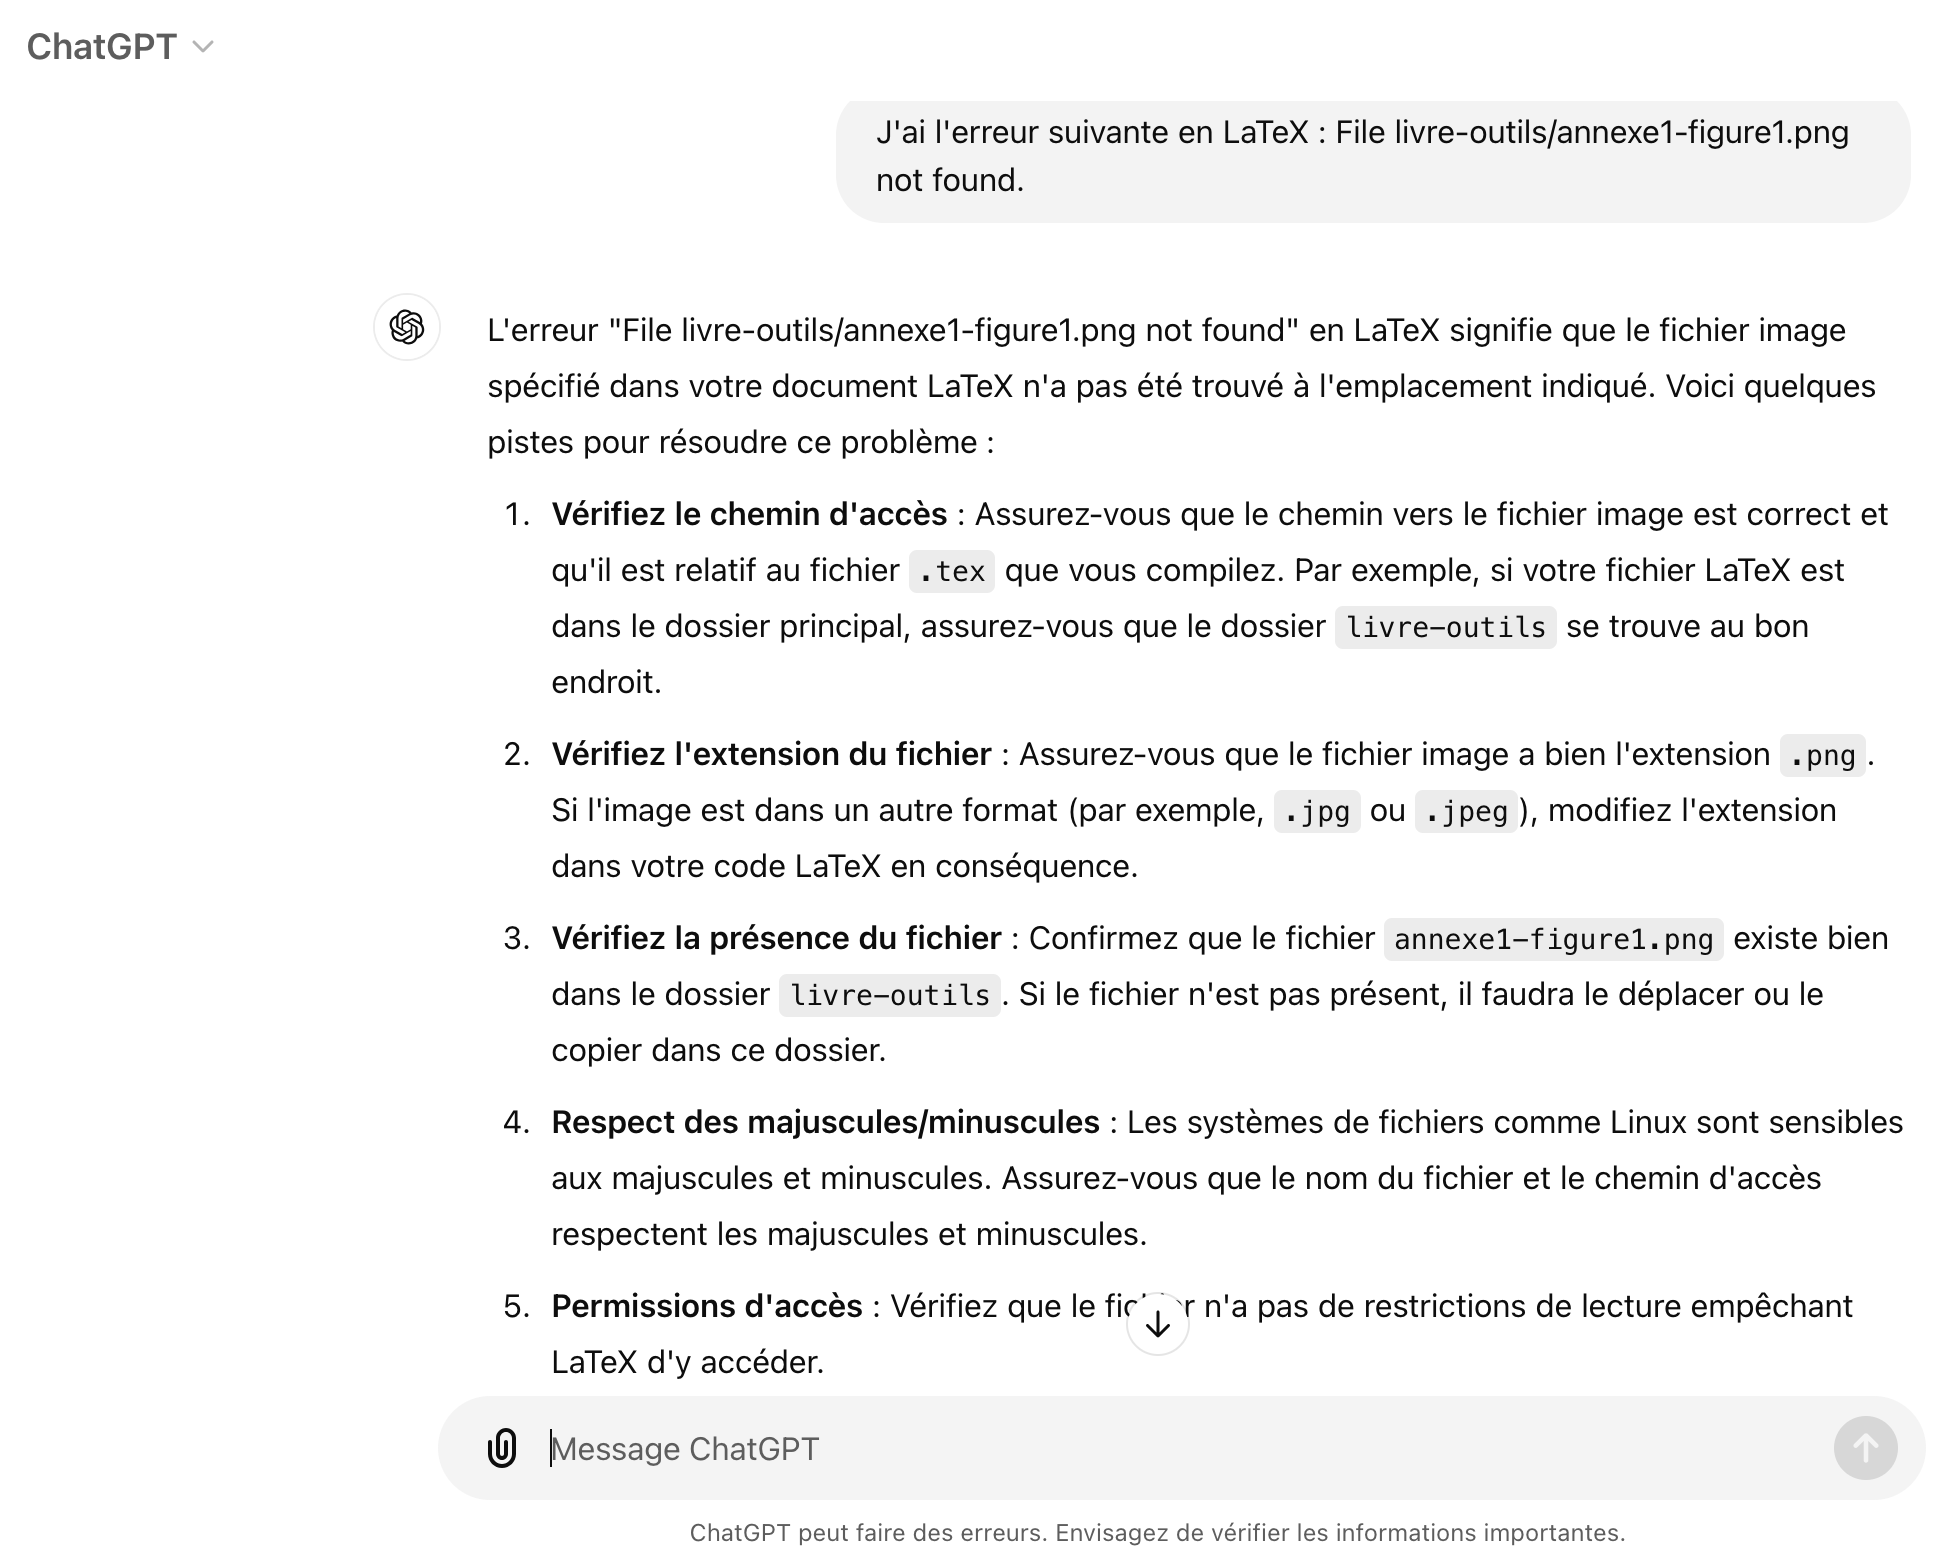
\includegraphics{images/chapitre7_gpt.png}

}

\caption{\label{fig-gpt}Exemple d'utilisation de ChatGPT pour une erreur
en code LaTeX \newline \textit{Source}~: Auteurs du présent chapitre.}

\end{figure}%

\subsubsection{Philosophie du code source ouvert et du logiciel
libre}\label{philosophie-du-code-source-ouvert-et-du-logiciel-libre}

L'utilisation des langages de balisage s'inscrit bien dans la
philosophie du logiciel libre. Le langage \LaTeX~est distribué sous la
license \LaTeX~project public license (LPPL), alors que Quarto 1.4 est
distribué sous la license du Massachusetts Institute of Technology
(MIT). Moyennant le respect de leurs licenses respectives, ces licenses
permettent ainsi aux utilisateurs de \LaTeX~et de Quarto d'utiliser ces
langages comme ils le souhaitent, de redistribuer des copies, de
modifier le fonctionnement de ces langages et d'en redistribuer des
versions améliorées. Bien que \LaTeX~et Quarto ne soient pas des
logiciels, leur license d'utilisation est cohérente avec la philosophie
du logiciel libre et permet à ces langages d'être utilisés dans de
nombreux logiciels.

D'autre part, \LaTeX~et Quarto sont deux langages à code source ouvert
(\emph{open source}). Ainsi, leur distribution est entièrement gratuite,
il n'y a rien à payer. Leur code source est disponible et les
changements à ce code doivent être indiqués. Les licences LPPL et MIT ne
discriminent pas certains groupes ou personnes, et elles ne restreignent
personne dans l'utilisation pour un domaine d'activité. Ces deux
licences ne sont pas spécifiques pour un produit, ce qui signifie que
ces deux langages peuvent être utilisés dans plusieurs logiciels et
programmes, dont certains sont payants --- Overleaf comporte ainsi une
version payante. Ces licences sont également technologiquement neutres,
rendant ainsi \LaTeX~et Quarto accessibles aux utilisateurs de tous les
systèmes d'exploitation.

\subsection{Inconvénients}\label{inconvuxe9nients}

Il existe toutefois des désavantages inhérents à l'utilisation des
langages de balisage. L'un des principaux désavantages de Markdown et de
\LaTeX~est le fait qu'ils ne comportent aucun système de suivi des
modifications lors de travaux collaboratifs. Pour réviser un travail
fait en langage de balisage, des commentaires peuvent être ajoutés sur
le fichier sortant --- nécessairement PDF pour un fichier sortant
produit avec \LaTeX. Des commentaires peuvent aussi être faits
directement dans le document \LaTeX~ou Markdown, à l'aide de balises
spécifiques. Ces commentaires n'apparaissent cependant pas dans le
fichier sortant. Le suivi des modifications en \LaTeX~et Markdown
nécessite donc souvent l'utilisation de Git et de GitHub, qui sont
abordés plus en détail dans le chapitre 3. Même avec une plateforme de
gestion des versions comme GitHub, les longs paragraphes ayant fait
l'objet de plusieurs modifications peuvent être longs à comparer par
rapport aux logiciels de traitement de texte, qui permettent de
visualiser les propositions d'ajouts et de retraits de caractères de
manière plus intuitive. Le suivi des modifications en logiciel de
traitement de texte permet également de distinguer les auteurs de
différents commentaires par leurs noms, alors que les ajouts et retraits
itératifs en GitHub peuvent rendre difficile l'identification de
l'auteur d'une modification. Pour ces raisons, et aussi pour faciliter
la mise en page par les éditeurs, certaines revues scientifiques
refusent les fichiers PDF et demandent que les soumissions soient faites
en format DOCX --- ce qui pose problème pour les utilisateurs de
\LaTeX~mais pas ceux de Markdown ou Quarto.

Les langages de balisage comportent également un autre désavantage
important dans certains cas : l'absence d'un correcteur de fautes de
français complet, en particulier pour corriger les fautes autres que
celles d'orthographe en français. Parmi les principaux endroits
permettant l'édition en langages de balisage, Visual Studio Code (VS
Code) et Overleaf comprennent tous deux une extension LanguageTool
(L\TeX pour VS Code, à ne pas confondre avec \LaTeX), qui permet la
révision orthographique et syntaxique dans plusieurs langues. VS Code
possède également une extension Antidote pour les personnes qui paient
déjà pour ce logiciel. D'autres extensions linguistiques existent
également pour VS Code, de même que pour les logiciels de traitement de
texte comme Word.

Positron, le nouvel IDE développé par Posit (les créateurs de RStudio)
et actuellement en version bêta au moment de la rédaction, représente
une option prometteuse pour l'édition de documents en langages de
balisage. Construit sur la même base technologique que VS Code, Positron
peut utiliser les mêmes extensions de vérification orthographique,
incluant potentiellement LanguageTool et d'autres correcteurs avancés.
De plus, l'équipe de développement a identifié le besoin d'offrir une
expérience d'écriture scientifique agréable dès l'installation, sans
avoir besoin d'installer des plugins (jmcphers, 2023), suggérant qu'un
système de vérification orthographique intégré pourrait être développé à
l'avenir.

Cependant, RStudio ne possède qu'un correcteur orthographique de base,
disponible en plusieurs langues. Ce correcteur ne repère pas les erreurs
de syntaxe, de grammaire ou de forme, entre autres. Ces éléments sont
pourtant essentiels pour la rédaction de textes académiques\footnote{Pour
  les utilisateurs de RStudio, il est souvent nécessaire de modifier le
  texte dans un logiciel de traitement de texte externe pour faire une
  révision linguistique complète, puis d'intégrer les corrections en
  collant le texte corrigé dans le document original en Markdown ou
  \LaTeX. Une application de bureau Grammarly peut également être
  intégrée sur RStudio. Cette application repère les erreurs de syntaxe,
  mais ne corrige que l'anglais, et certains soucis de repérage des mots
  aux bons endroits dans le texte en rendent présentement l'utilisation
  difficile.}, d'autant plus que les utilisateurs de \LaTeX ont tendance
à faire davantage de fautes d'orthographe et de grammaire lors de la
rédaction que les utilisateurs de Word (Knauff \& Nejasmic, 2014). Bien
que RStudio soit excellent pour la programmation en R et l'analyse de
données, les auteurs du présent ouvrage suggèrent fortement que les
utilisateurs des langages de balisage fassent appel à VS Code, Positron,
ou Overleaf plutôt qu'à RStudio pour l'édition de leurs documents, afin
de profiter d'extensions de correction grammaticale plus complètes comme
LanguageTool/L\TeX. Une approche hybride -- RStudio pour l'analyse de
données, Positron/VS Code/Overleaf pour la rédaction -- peut s'avérer
particulièrement efficace.

Enfin, les langages de balisage, contrairement aux logiciels de
traitement de texte, nécessitent d'être compilés, ce qui implique que
deux fichiers coexistent~: le fichier où le langage de balisage est
utilisé --- format \texttt{.tex} pour \LaTeX, \texttt{.md} pour Markdown
ou encore \texttt{.qmd} pour Quarto --- ainsi que le fichier où le texte
final balisé apparait --- généralement \texttt{.pdf}, \texttt{.docx} ou
\texttt{.html}. La compilation peut prendre un temps variable selon la
complexité du document, mais dure typiquement une quinzaine de secondes.
Le fait de devoir travailler avec deux fichiers en parallèle et de ne
pas voir immédiatement l'effet des balises sur le document final
constitue ainsi un autre désavantage des langages de balisage.

\LaTeX~comporte aussi quelques difficultés techniques particulières qui
peuvent être réglées ou diminuées en travaillant en Markdown.
Premièrement, \LaTeX~est difficile à apprendre. Certaines tâches qui
peuvent sembler simples comme l'ajout d'un tableau peuvent nécessiter de
nombreuses lignes de code. De plus, à la moindre erreur de frappe dans
l'utilisation d'une balise, le code risque de ne pas fonctionner et de
ne pas produire le document PDF souhaité. C'est ce qu'on appelle une
erreur de compilation. Markdown est un langage plus simple à apprendre,
avec des balises plus courtes et intuitives. Il occasionne donc moins
d'erreurs de compilation.

Deuxièmement, \LaTeX est peu compatible avec les logiciels de traitement
de texte comme Word. Dans un sens, pour transférer un fichier créé à
partir d'un logiciel de traitement de texte vers \LaTeX, les balises
doivent être ajoutées manuellement une par une. Dans l'autre sens, pour
transférer un document \LaTeX vers un fichier de traitement de texte, le
convertisseur Pandoc peut être utilisé, mais celui-ci ne repère pas
toutes les balises. Il est alors souvent nécessaire de faire des
aller-retour entre le fichier \LaTeX original et le fichier converti en
format DOCX pour s'assurer du succès de la conversion. Parfois, les
balises doivent même être retirées une par une et le formatage doit être
refait en utilisant les boutons fournis sur le logiciel de traitement de
texte. Une autre option consiste à copier le texte directement à partir
du fichier PDF produit par \LaTeX vers un logiciel de traitement de
texte, mais cette méthode présente aussi des défis : les fins de ligne
sont interprétées par Word, Pages ou Writer comme des retours plutôt que
des espaces, et les accents sont souvent mal copiés et doivent être
réécrits manuellement.

Markdown et Quarto évitent en grande partie ce problème en permettant
d'écrire un fichier DOCX à partir du langage de balisage. Le formatage
du fichier DOCX demeure un peu compliqué cependant et doit être fait à
partir du modèle d'un autre document DOCX formaté tel que souhaité.
Quarto facilite particulièrement cette tâche en permettant d'écrire un
texte en format Markdown et de produire un fichier DOCX à partir d'un
gabarit Word. Cependant, les fichiers DOCX ne peuvent toujours pas être
transformés en format Markdown. Pour les fichiers Word à transformer en
format Markdown, les balises plus simples en Markdown qu'en
\LaTeX rendent néanmoins la tâche plus simple.

Somme toute, Word n'est pas à antagoniser et demeure très utile pour des
tâches simples. Cependant, dans le monde académique, la production de
fichiers de qualité faisant appel à des graphiques, tableaux et blocs de
code personnalisés de qualité et automatisés est simplifiée en utilisant
des langages de balisage. Il n'est ainsi pas anodin que ces langages
soient adoptés par plusieurs dans le monde académique, surtout pour la
rédaction de manuscrits au formatage très strict comme des mémoires et
des thèses --- plusieurs universités possèdent ainsi que gabarits
\LaTeX de mémoires et de thèses. Pour ces raisons, il est avantageux
pour une personne poursuivant des études supérieures en sciences
sociales, par exemple, de passer outre la difficulté initiale
d'apprentissage des langages de balisage. L'apprentissage de ces
langages permettra de s'aligner sur les pratiques répandues dans le
milieu académique et d'améliorer davantage la qualité de la production
d'écrits scientifiques.

\section{Manuel d'instructions~: comment utiliser un langage de
balisage?}\label{manuel-dinstructions-comment-utiliser-un-langage-de-balisage}

En pratique, comment utilise-t-on Markdown, \LaTeX~et \textsc{Bib}\TeX?
D'emblée, \LaTeX~a une syntaxe particulière qui demande un certain temps
d'adaptation. Pour écrire une phrase simple comme celle-ci, la phrase
peut être écrite telle quelle. Par contre, pour mettre un \textbf{mot}
en caractères gras, il faut utiliser la balise suivante~:
\texttt{\textbackslash{}textbf\{mot\}}. Pour mettre le
\textcolor{red}{mot} en rouge, la balise est
\texttt{\textbackslash{}textcolor\{red\}\{mot\}}. Pour le mettre en
italique et en note de bas de page\footnote{\emph{mot}}, les balises
\texttt{\textbackslash{}footnote\{\textbackslash{}emph\{mot\}\}} peuvent
être utilisées. Ainsi, des balises peuvent contenir d'autres balises. En
langage \LaTeX, une balise commence toujours par une barre oblique
inversée. Par la suite, le nom de la fonction --- \emph{emph},
\emph{textbf}, \emph{textcolor}, etc. --- est appelé. Enfin,
généralement, le mot à formater est placé entre accolades
(\texttt{\{\}}).

Chaque document \LaTeX{} commence par un préambule. Celui-ci présente
des informations telles que la taille des caractères, le type de
document, le format de mise en page, la police de caractères,
l'utilisation d'en-têtes et de pieds de page, ainsi que l'utilisation de
\emph{packages} \LaTeX~permettant différentes fonctionnalités de
personnalisation du document. Il n'est pas nécessaire ni souhaitable
d'apprendre l'ensemble des fonctions et des \emph{packages} \LaTeX~qui
existent. Au contraire, il est souvent mieux pour l'utilisateur de
commencer par un gabarit de document qui convient au type de document
désiré et ensuite de rechercher en anglais sur Stack Overflow la manière
d'ajouter des éléments de formatage qui lui sont inconnus, par exemple
en recherchant \texttt{highlight\ latex\ text}.

Markdown fonctionne de manière similaire à \LaTeX, mais se démarque par
sa plus grande flexibilité et sa syntaxe beaucoup plus légère. Par
contre, il nécessite parfois l'utilisation de balises \LaTeX~afin de
réaliser certaines tâches, comme changer la couleur du texte. Tout
document Markdown débute avec un court bloc de syntaxe YAML (acronyme de
\emph{Yet Another Markup Language}) qui définit les paramètres généraux
du document. Voici un bloc YAML typique pour un document Quarto~:

\begin{verbatim}
---
title: "Baliser les sciences sociales"
subtitle: "Langages et pratiques"
date: today
author:
  - Alexandre Fortier-Chouinard^[University of Toronto]
  - Étienne Proulx^[Université Laval]
  - Maxime Blanchard^[McGill University]
format: pdf
toc: true
date-format: "MMMM D, YYYY"
bibliography: other_files/livre-outils.bib
---
\end{verbatim}

Outre le titre, le sous-titre et le nom des auteurs, on trouve aussi
dans l'en-tête YAML la présence d'une table des matières (\texttt{toc}),
la date et son format, le format du document compilé --- dans ce cas-ci,
PDF --- ainsi que le chemin d'arborescence afin d'accéder au document
\textsc{Bib}\TeX~où sont enregistrées les références utilisées. Il est
aussi possible d'y définir la taille de la police de caractères ou
encore le gabarit Word servant à définir le format d'un document DOCX à
produire. De manière particulièrement importante, l'entête YAML est
l'endroit où sont chargés les \emph{packages} \LaTeX~qui seront
utilisés. En effet, la majorité des \emph{packages} et fonctions
\LaTeX~sont utilisables dans Markdown, alors que l'inverse n'est pas
vrai. Il est donc possible de personnaliser un document Markdown en
utilisant des \emph{packages} ayant été créés pour \LaTeX.

La syntaxe à utiliser au travers du texte en Markdown est somme toute
plutôt simple. Pour mettre un ou plusieurs \textbf{mots en gras}, il
suffit de les entourer de deux astérisques
(\texttt{**mots\ en\ gras**}); pour les mettre \emph{en italique}, il
faut les encadrer d'une seule astérisque (\texttt{*en\ italique*}). Pour
définir un titre de section ou de sous-section, il suffit de mettre des
\texttt{\#} devant le titre en question. Plus on ajoute de \texttt{\#},
plus le titre sera petit et plus il sera considéré à un niveau
hiérarchique inférieur dans la structure du texte. La syntaxe Markdown
est donc plus légère que celle de \LaTeX, dans le but d'en rendre la
lecture plus simple pour les utilisateurs et utilisatrices.

Bien que des gabarits Markdown soient disponibles, ceux-ci sont plus
rares. Ils se trouvent pour la plupart sur GitHub et sont rendus
disponibles par leur créateur. Cela étant dit, leur personnalisation
peut s'avérer plutôt complexe. En somme, Markdown est particulièrement
pratique pour les documents ne nécessitant pas de respecter un gabarit
précis et requérant simplement un document d'allure simple et
professionnelle.

Pour sa part, \textsc{Bib}\TeX~a une syntaxe relativement simple.
D'emblée, les références \textsc{Bib}\TeX pour des articles et ouvrages
scientifiques sont disponibles sur Google Scholar. La
Figure~\ref{fig-ggscholar} montre comment accéder facilement à ces
références. Toutefois, pour citer des sites Web ou des articles de
médias, la référence doit être écrite à la main selon un format précis.
Une bibliographie sur \textsc{Bib}\TeX~peut ressembler à ceci~:

\begin{verbatim}
@book{darwin03,
  address = {London},
  author = {Darwin, Charles},
  publisher = {John Murray},
  title = {{On the Origin of Species by Means of Natural Selection
or the Preservation of Favoured Races in the Struggle for Life}},
  year = {1859}
}

@article{goldfarb96,
  title={The Roots of SGML: A Personal Recollection},
  author={Goldfarb, Charles F},
  journal={Technical communication},
  volume={46},
  number={1},
  pages={75},
  year={1999},
  publisher={Society for Technical Communication}
}
\end{verbatim}

\begin{figure}

\centering{

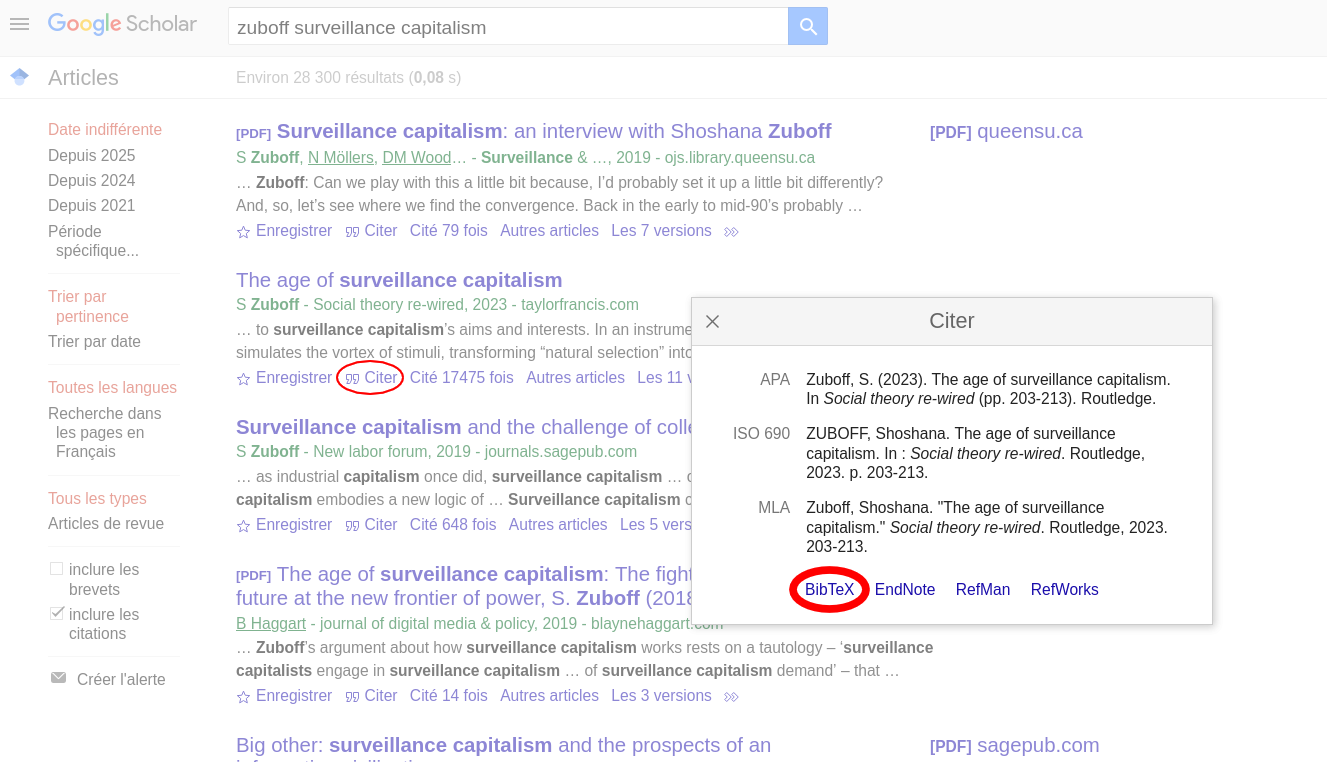
\includegraphics[width=1\textwidth,height=\textheight]{images/chapitre7_google_scholar_bibtex.png}

}

\caption{\label{fig-ggscholar}Capture d'écran d'un exemple illustrant
comment trouver le \textsc{Bib}\TeX~sur Google
Scholar.\newline \textit{Source}~: Auteurs du présent chapitre.}

\end{figure}%

Un fichier \textsc{Bib}\TeX~ne contient rien de plus qu'une série de
publications commençant chacune par la balise \texttt{@} suivie du type
d'article --- \emph{article}, \emph{book} pour un livre,
\emph{incollection} pour un chapitre de livre, \emph{inproceedings} pour
une présentation dans une conférence, \emph{unpublished} pour un article
non publié et \emph{online} pour un site Web sont parmi les plus connus
--- et des informations sur la publication mises entre accolades. La
première information entre accolades est le code de la référence, par
exemple \texttt{goldfarb96}. Dans le fichier \LaTeX, l'auteur doit
écrire \texttt{\textbackslash{}cite\{goldfarb96\}} pour voir dans le
document PDF compilé Goldfarb (1996); le lien est automatiquement
cliquable et renvoie à la notice bibliographique correspondante. L'ordre
des publications dans le document \textsc{Bib}\TeX~a peu d'importance,
puisque \LaTeX~réordonne par défaut la bibliographie en ordre
alphabétique.

\subsection{Environnements d'édition et de
compilation}\label{environnements-duxe9dition-et-de-compilation}

Contrairement à Microsoft Word et Apple Pages, il existe plusieurs
options d'environnements d'édition et de compilation spécifiques à
chaque langage. Ces environnements sont des plateformes et des logiciels
conçus pour faciliter l'édition, la mise en forme et la compilation de
documents dans des langages de balisage tels que \LaTeX~et Markdown. Ils
permettent également de rendre plus efficace et conviviale la production
de documents tout en fournissant des fonctionnalités spécifiques aux
besoins de chaque langage. Il existe une grande diversité
d'environnements d'édition et de compilation, et le choix est libre pour
la chercheuse ou le chercheur de trouver celui qui convient le mieux à
ses besoins ou aux besoins de son groupe de recherche. Les trois options
discutées ici sont parmi les plus utilisées par les chercheurs en
sciences sociales et peuvent être regroupées en deux catégories~: les
logiciels de bureau et les éditeurs en ligne. La
Figure~\ref{fig-environnements-edition} présente une vue d'ensemble des
principaux environnements d'édition disponibles pour les chercheurs en
sciences sociales, organisés selon leur type (logiciels de bureau vs
éditeurs en ligne) et les langages de balisage qu'ils supportent.

\begin{figure}

\centering{

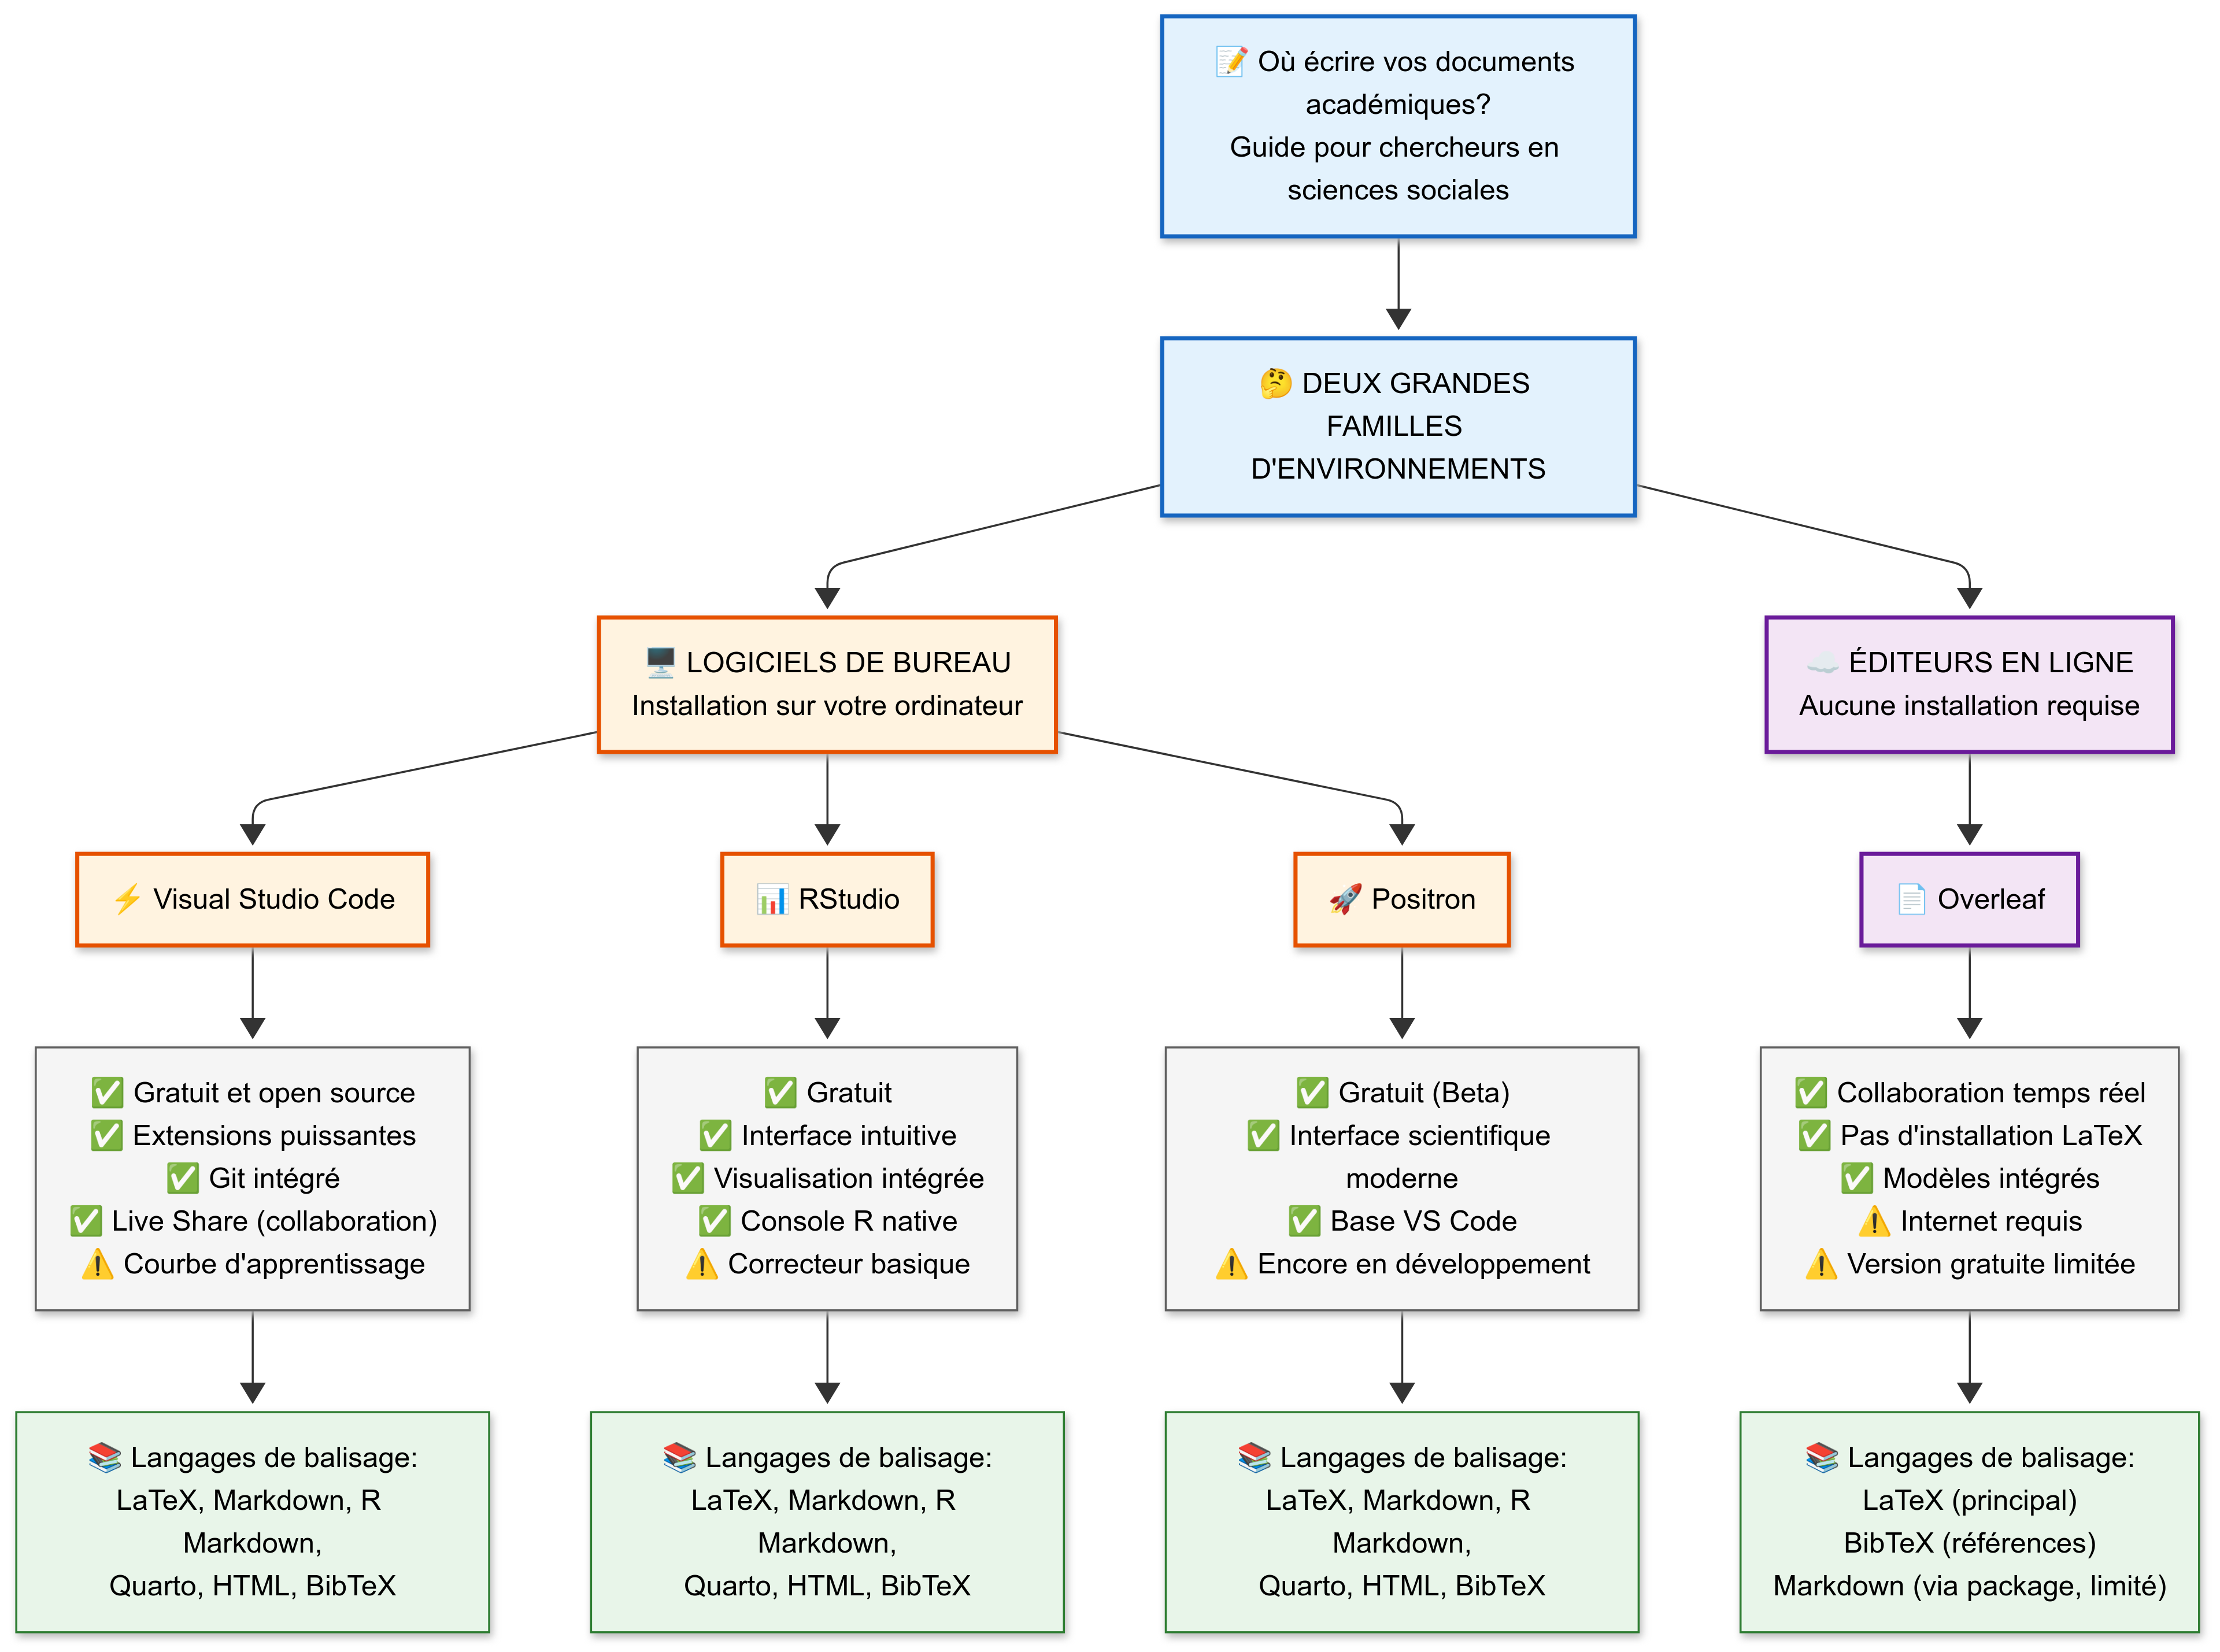
\includegraphics[width=0.9\textwidth,height=\textheight]{images/chapitre7_mermaid2.png}

}

\caption{\label{fig-environnements-edition}Vue d'ensemble des
environnements d'édition pour langages de balisage
\newline \textit{Source}~: Auteurs du présent chapitre.}

\end{figure}%

D'abord, il existe plusieurs logiciels de bureau qui offrent un
environnement d'édition et/ou de compilation pour les langages de
balisage. Ces logiciels fournissent les programmes principaux, les
extensions essentielles et des outils complémentaires de compilation et
de visualisation afin de permettre la production de documents écrits en
langages de balisage. Deux environnements régulièrement utilisés pour
travailler en langage de balisage sont le logiciels de bureau VS Code et
RStudio, également abordé dans le chapitre 2. VS Code prend en compte un
plus grand nombre de langages de programmation et est utilisé par les
programmeurs de tous domaines, tandis qu'RStudio est surtout utile pour
les chercheurs en sciences sociales qui travaillent surtout en
\texttt{R}.

Utiliser VS Code ou RStudio pour travailler en langage de balisage
permet de produire des documents avec différents langages de balisage et
programmation, ainsi que de naviguer entre eux, à partir d'une même
fenêtre. Il suffit d'installer certains \emph{packages} contenant les
fichiers nécessaires à l'utilisation des langages de balisage. Par
exemple, il est possible de produire des documents en \LaTeX~en
utilisant le code suivant dans la console pour installer le
\emph{package} nécessaire à l'utilisation de la distribution
\LaTeX~Tiny\TeX\footnote{Outre Tiny\TeX, il existe d'autres
  distributions telles que Mac\TeX~pour Mac et Mik\TeX~pour Windows
  (Just, 2013). Ces distributions se distinguent par les différents
  \emph{packages} avec lesquelles elles sont compatibles.}~:
\texttt{install.packages("tinytex")}. Pour l'écriture en langage de
balisage, il est en effet nécessaire d'installer l'une des nombreuses
distributions \LaTeX~en ligne afin de pouvoir compiler ces documents
dans un environnement local. Suivant le même principe, il est possible
de produire des documents en \texttt{R} Markdown sur RStudio en
installant le \emph{package} suivant~:
\texttt{install.packages("rmarkdown")}. Pour Quarto, le téléchargement
se fait en ligne, directement à partir du site Web de Quarto (2023).

Lorsque vient le temps de collaborer à plusieurs sur un document écrit
en Markdown ou en \LaTeX, les logiciels de bureau évoqués précédemment
nécessitent l'utilisation de GitHub et de Git. L'utilisation de ces
éditeurs peut présenter un défi supplémentaire pour les équipes de
recherche non initiées. Il existe ainsi des éditeurs en ligne qui
permettent de collaborer en temps réel sans passer par Git et GitHub, de
manière similaire à Google Docs. Le plus connu de ces éditeurs en ligne
est Overleaf, qui permet de produire des documents en langage
\LaTeX\footnote{VS Code possède également une extension, Live Share, qui
  permet de travailler en temps réel sur un même document.}.
Puisqu'Overleaf permet d'avoir accès à ses documents \LaTeX~à partir de
n'importe quel navigateur, il n'y a pas de dépendance à un logiciel
local sur un ordinateur, ce qui constitue un avantage important. La
contrepartie de cet avantage est qu'en utilisant Overleaf, l'équipe de
recherche est dépendante d'une connexion à Internet. En utilisant le
package \LaTeX~\texttt{rmarkdown}, Overleaf peut également inclure du
code Markdown. Cependant, Overleaf ne permet pas de créer des documents
en format DOCX ou HTML, ce qui constitue une limite de l'application.
Overleaf comporte un compteur de mots intégré, ce qui n'est pas le cas
des logiciels et environnements présentés plus haut.

\section{Conclusion~: pièges et
astuces}\label{conclusion-piuxe8ges-et-astuces}

Maintenant que le lecteur de ce chapitre a une meilleure idée de ce que
sont les langages de balisage et de leur utilité, la prochaine étape
consiste à expérimenter par lui-même. Le chapitre se termine donc par un
résumé des étapes à suivre pour devenir expert dans les langages de
balisage.

La première étape consiste à commencer à expérimenter dès que possible,
sans se laisser freiner par l'incompréhension. Il n'est pas nécessaire
de tout comprendre des langages de balisage pour produire un document de
qualité. Avec cet état d'esprit, il franchira les difficultés initiales
de l'apprentissage des langages de balisage plus rapidement. Avant de
commencer, il doit s'assurer d'avoir un ordinateur de bonne qualité qui
lui permet de travailler rapidement (voir l'Annexe I à ce sujet).

En deuxième lieu, il ne faut pas hésiter à utiliser les ressources
disponibles pour gagner du temps. Les \emph{cheat sheets} disponibles en
ligne, l'aide de LLMs qui connaissent les langages de balisage (par
exemple, ChatGPT) et le recours à des sites comme Stack Overflow peuvent
être très utiles. Si on ne fait pas appel à des ressources externes, il
peut être facile de devenir fâché contre soi-même ou contre
l'infrastructure informatique. Il est parfaitement normal de demander de
l'aide externe. Même les experts le font.

La troisième étape est de ne surtout pas sous-estimer l'aide de ses
pairs. Il ne faut pas hésiter à poser des questions et à demander de
l'aide à des personnes plus expérimentées pour résoudre des problèmes
que l'on ne parvient pas à résoudre avec les ressources externes.

Avant d'aborder la quatrième et dernière étape, il est important de
mentionner quelques pièges à éviter lors de la transition de débutant à
expert. Tout d'abord, faites attention aux exigences des revues
lorsqu'il soumet des articles scientifiques. Certaines demandent des
articles au format Word tandis que d'autres préfèrent les langages de
balisage. Savoir comment convertir correctement les documents est donc
un atout.

De plus, il ne faut pas se limiter à un seul langage de balisage et se
montrer polyvalent, car travailler en collaboration peut nécessiter de
s'adapter aux pratiques des partenaires. Il faut également éviter les
erreurs lors de la compilation des documents écrits en langage de
balisage en portant une attention particulière aux balises et en ne les
laissant pas s'accumuler. Une bonne façon de veiller à ce que les
erreurs ne s'accumulent pas est de compiler fréquemment les documents en
cours de production.

Un des pièges qui peut sembler évident, mais qui mérite d'être répété,
est l'attention portée à la qualité de la langue écrite. L'utilisateur
doit être à l'affût de la présence de correcteurs automatiques ou non
dans ses environnements d'édition. S'il y en a un, il faut aussi
vérifier si ce correcteur automatique est dans la bonne langue (français
canadien, anglais canadien, etc.).

Enfin, il faut éviter les conflits Git lors de la collaboration sur
GitHub en coordonnant efficacement les travaux d'équipe et en utilisant
Git de manière optimale pour tirer parti des langages de balisage. Il
est donc important de se renseigner quant aux bonnes pratiques à suivre
afin de collaborer efficacement avec Git. À cet égard, la section 3.3 du
chapitre 3 présente un guide détaillé des meilleures pratiques pour
utiliser Git et GitHub dans un contexte de recherche collaborative.

Pour conclure, la dernière étape pour devenir expert en langages de
balisage est d'être créatif. Il est recommandé d'explorer les
différentes balises et de les utiliser de manière inventive. Les
langages de balisage permettront d'effectuer des tâches que
l'utilisateur n'aurait pas pu réaliser facilement en utilisant un
logiciel de traitement de texte classique. Ils permettront de produire
des documents professionnels dans différents formats personnalisés,
produits avec des processus automatisés, avec une grande qualité
graphique.

\bookmarksetup{startatroot}

\chapter{Outils d'intelligence artificielle}\label{sec-chap8}

\begin{center}

Jozef Rivest, Laurence-Olivier Foisy, Hubert Cadieux

\end{center}

Ce chapitre vise à initier les lecteurs à ce qu'est l'intelligence
artificielle (IA), aux enjeux qu'elle engendre ainsi qu'à son potentiel
pour les sciences sociales. Dans un premier temps, et en trame de fond
de ce chapitre, les lecteurs seront appelés à développer leurs
intuitions dans leur utilisation de différents outils de l'IA. Avant
tout, au moment d'écrire ces lignes, il est important de mentionner que
l'étude de l'IA dans les sciences sociales est encore jeune. Par
conséquent, beaucoup de questions restent encore en suspend. Face à ce
constat, il est important de développer son regard critique afin
d'orienter son utilisation de l'IA. Se poser des questions et tenter de
trouver des réponses ne peut que générer des bénéfices. Ainsi, si ce
chapitre permet d'éclairer certains enjeux, ou s'il stimule davantage de
questionnement, alors il aura réussi son objectif.

Dans un deuxième temps, ce chapitre vise à présenter certains outils de
l'IA qui s'inscrivent dans les grandes étapes de la recherche. Il est
important de mentionner que ces outils évoluent à une vitesse
impressionnante. Par conséquent, certaines fonctionnalités présentées
dans ce chapitre peuvent possiblement changer dans les prochaines
années. Les lecteurs sont appelés à consulter les dernières mises à jour
de ces outils afin de connaître les derniers changements et les
nouvelles fonctionnalités. Bien qu'il soit difficile de catégoriser ces
outils de manière exclusive dans chacune de ces catégories, un certain
ordre d'utilisation est proposé. Celui-ci est surtout illustratif afin
de présenter les fonctionnalités principales. Cependant, les lecteurs
sont appelés à réfléchir à propos de l'intégration de ces outils dans
leur flux de travail en fonction de leur besoin.

La section point d'observation présentera une définition de l'IA,
l'évolution de cette dernière dans les dernières années ainsi que la
présence et l'utilisation de l'IA dans les sciences sociales. Ensuite,
la section arpentage et choix éditoriaux présentera différents outils de
l'IA qui s'insèrent bien dans les diffèrentes étapes de la recherche, de
la conception jusqu'à la publication des réusltats. Finalement, avant de
conclure le chapitre, il est intéressant de se demander ce que devient
le chercheur à l'aube de cette révolution technologique.

\section{Point d'observation:}\label{point-dobservation}

\subsection{Définition et différents types
d'IA}\label{duxe9finition-et-diffuxe9rents-types-dia}

Qu'est-ce que l'IA ? Est-ce quelque chose d'homogène, ou s'agit-il
plutôt « des intelligences artificielles »? Dans un premier temps, il
est important de préciser que l'IA est un champ d'études (Devedzic,
2022). Par conséquent, il s'agit d'un ensemble d'objets, relativement
vaste et en constante expansion, qui s'intéresse, à sa façon, à l'IA.
Pour préciser ce propos, prenons l'exemple de la science politique.
Malgré la formulation au singulier, la science politique est un grand
ensemble de différents sous-champs d'études, qui ont chacun leur propre
objet d'intérêt. La philosophie politique, les relations
internationales, la politique comparée et l'étude de l'opinion publique,
par exemple, sont tous des sous-champs qui s'intéressent, à leur façon,
au phénomène politique. Dans le même sens, et compte tenu de cette
pluralité de perspectives, il est important de noter qu'il n'y a pas de
consensus dans la définition de l'IA (König et al., 2022; Wang, 2019).
De plus, la rapidité du développement de ce champ rend le traçage de
frontières définitionnelles plutôt difficile : comment définir, d'une
manière précise et consensuelle, quelque chose qui évolue constamment
(Bertolini, 2020, pp.~15; Devedzic, 2022)?

Deux définitions de l'IA peuvent tout de même être retenues. La première
vient de John McCarthy (2007, pp.~2) : « Il s'agit de la science et de
l'ingénierie qui consistent à créer des machines
intelligentes\footnote{Intelligence étant défini de la façon suivante :
  « L'intelligence est la partie informatique de la capacité à atteindre
  des objectifs dans le monde. On trouve différents types et degrés
  d'intelligence chez l'homme, chez de nombreux animaux et chez
  certaines machines. » (McCarthy, 2007, pp.~2)}, en particulier des
programmes informatiques intelligents. Elle est liée à la tâche
similaire consistant à utiliser des ordinateurs pour comprendre
l'intelligence humaine, mais l'IA ne doit pas se limiter aux méthodes
qui sont biologiquement observables. »\footnote{Toutes les traductions
  ont été effectuées par le logiciel DeepL}. La seconde définition
provient de la compagnie IBM (2023a) : « Dans sa forme la plus simple,
l'IA est un domaine qui combine l'informatique et des ensembles de
données robustes pour permettre la résolution de problèmes. Elle englobe
également les sous-domaines de l'apprentissage automatique et de
l'apprentissage profond, qui sont souvent mentionnés en conjonction avec
l'IA. Ces disciplines sont composées d'algorithmes d'IA qui cherchent à
créer des systèmes experts qui font des prédictions ou des
classifications basées sur des données d'entrée ». Ces extraits
permettent de comprendre que l'IA consiste à reproduire artificiellement
certaines capacités cognitives humaines, afin de rendre les machines «
intelligentes » en leur donnant la capacité de résoudre des problèmes
par elles-mêmes.

Ces définitions restent toutefois à préciser, notamment dans le champ
d'application de l'IA : qu'en est-il concrètement ? Comment est-ce
utilisé ? Comment ça fonctionne ? Si l'IA se distingue en plusieurs
types, en faire la liste et identifier leurs différentes branches et
applications possibles serait fastidieux et s'écarterait de l'objectif
de ce chapitre introductif. Cependant, pour ceux désirant en savoir plus
sur le sujet, les articles de McCarthy (2007) et de Hanchen et al.
(2023), ainsi que le Cambridge Handbook of Artificial Intelligence
(König et al., 2022) sont très riches et illustratifs.

Avant toute chose, il est important de distinguer l'IA général (strong)
du précis (narrow). Le premier, et le moins populaire en nombre de
recherches et d'applications, cherche à développer une machine qui
aurait les mêmes capacités cognitives que l'humain, non seulement en
termes de résolution de problème, d'apprentissage et de planification,
mais aussi qui serait dotée d'une conscience de soi (IBM, 2023a; König
et al., 2022). Le deuxième est plus restrictif, se limitant à la
réalisation d'un ou de plusieurs objectifs spécifiques. De ces deux
visées, il y a trois principaux champs de recherche qui se penchent sur
les méthodes de fonctionnement de l'IA : l'apprentissage machine
(machine learning), les réseaux neuronaux artificiels (artificial neural
networks) ainsi que l'apprentissage profond (deep learning).

L'apprentissage machine :

\begin{singlespacing} \begin{displayquote} « [...] consiste à
programmer des ordinateurs pour optimiser un critère de performance
à l'aide de données d'exemple ou d'expériences passées. Nous avons
un modèle défini jusqu'à certains paramètres, et l'apprentissage
est l'exécution d'un programme informatique pour optimiser les
paramètres du modèle à l'aide des données d'entraînement ou de
l'expérience passée » (Alpaydin et Bach 2014, pp. 3).  \end{displayquote}
\end{singlespacing}

Le but est d'entraîner le modèle afin qu'il puisse reconnaître des
tendances, et qu'il puisse décrire et/ou faire des prédictions à partir
de ces tendances (Alpaydin \& Bach, 2014, pp.~3). Il est le champ le
plus populaire dans la recherche faite sur l'IA, notamment parce qu'il
constitue une base importante pour les autres recherches dans le domaine
(Devedzic, 2022).

Ensuite, un sous-champ de l'apprentissage machine, l'apprentissage
profond, « {[}\ldots{]} fait référence à un réseau neuronal composé de
plus de trois couches {[}\ldots{]}. L'apprentissage en profondeur
automatise une grande partie de l'extraction des caractéristiques,
éliminant ainsi une partie de l'intervention humaine manuelle nécessaire
et permettant l'utilisation d'ensembles de données plus importants. Il
peut ingérer des données non structurées dans leur forme brute et
déterminer automatiquement la hiérarchie des caractéristiques qui
distinguent les différentes catégories de données les unes des autres,
ne nécessitant pas d'intervention humaine. » (IBM, 2023a). Ainsi,
l'apprentissage profond permet une certaine forme d'automatisation des
tâches demandées à l'IA, en lui fournissant les capacités nécessaires
d'apprendre par lui-même pour corriger et améliorer son fonctionnement.
Pour ce faire, on doit développer des structures neuronales
artificielles, qui s'inspirent des neurones du cerveau humain.

C'est d'ailleurs la tâche de ceux qui s'intéressent aux réseaux
neuronaux artificiels : « Les réseaux neuronaux artificiels (RNA) sont
constitués d'une couche de nœuds, contenant une couche d'entrée, une ou
plusieurs couches cachées et une couche de sortie. Chaque nœud, ou
neurone artificiel, se connecte à un autre et possède un poids et un
seuil associés. Si la sortie d'un nœud individuel est supérieure à la
valeur seuil spécifiée, ce nœud est activé et envoie des données à la
couche suivante du réseau. Dans le cas contraire, aucune donnée n'est
transmise à la couche suivante du réseau » (IBM 2023b). Ainsi, le but
est de reproduire les structures cognitives humaines, afin de permettre
à l'IA d'accomplir des tâches plus complexes. L'une des principales
utilités de ce sous-champ est qu'il permet d'augmenter la rapidité du
classement de données ; la reconnaissance vocale ou d'image, par
exemple, ne prend que quelques minutes grâce à cela, contrairement à
plusieurs heures, lorsque fait par des humains (IBM, 2023b).

\subsection{L'évolution constante de
l'IA}\label{luxe9volution-constante-de-lia}

Plusieurs chercheurs, dont le professeur Yoshua Bengio de l'Université
de Montréal, ont lancé plusieurs avertissements sur le développement de
l'IA, notamment à cause de la rapidité de son évolution. Dans un article
paru dans The Economist, Dr.~Bengio (2023) déclare qu'il prévoyait le
développement d'une IA avec des capacités similaires à celles de
l'humain d'ici quelques décennies, peut-être un siècle. Depuis l'arrivée
de ChatGPT-4, celui-ci a revu sa prédiction pour la situer entre
quelques années et quelques décennies (Bengio, 2023). Dans les dix
dernières années seulement, les systèmes de reconnaissance d'images et
de langages en sont venus à dépasser les capacités humaines (Roser,
2022). La Figure~\ref{fig-evolution} présente cette évolution.

\begin{Shaded}
\begin{Highlighting}[]
\FunctionTok{source}\NormalTok{(}\StringTok{"chapitre\_8\_file/graphique.R"}\NormalTok{)}
\end{Highlighting}
\end{Shaded}

\begin{verbatim}
Warning: Using `size` aesthetic for lines was deprecated in ggplot2 3.4.0.
i Please use `linewidth` instead.
\end{verbatim}

\begin{Shaded}
\begin{Highlighting}[]
\NormalTok{ai\_evolution}
\end{Highlighting}
\end{Shaded}

\begin{figure}[H]

\centering{

\includegraphics{chapitre_8_files/figure-pdf/fig-evolution-1.pdf}

}

\caption{\label{fig-evolution}}

\end{figure}%

Comme on le remarque, cette évolution ne suit pas une trajectoire
linéaire. Depuis 2015, la plupart de ces technologies ont évolué de
manière quasi exponentielle. Cette progression fulgurante nous permet de
faire quelques constats pour appréhender l'évolution future. Tout
d'abord, le développement dans les capacités de l'IA permet d'accélérer
de manière exponentielle le champ dans son ensemble, ce qui rend cette
technologie exponentiellement plus puissante (Harari, 2023). Elle est
capable de se faire évoluer à une vitesse plus grande, grâce à ses
capacités de traitement de données et d'auto améliorations, que si elle
était uniquement dépendante de l'humain.

En tant que chercheur en sciences sociales, pourquoi devrait-on être
préoccupé par le développement de l'IA? Tout d'abord, il est important
de commencer à réfléchir ainsi qu'à analyser les différents impacts que
l'IA a sur nos sociétés. Les avancer dans le domaine en plus de
l'accessibilité à ces technologies, tel que Large Language Model (LLM),
en font de nouveaux objets d'étude qui génèrent beaucoup de questions.
Yuval Noah Harrari (2023), historien et philosophe, explique dans un
article que la capacité de l'IA à manipuler ainsi qu'à générer du
langage en fait un outil puissant qui a le potentiel d'avoir de profonds
impacts sur nos civilisations. Par conséquent, l'étude des effets de
l'IA sur nos sociétés devient un nouveau sujet de recherche dont tous
les champs des sciences sociales et sciences humaines ont intérêt à se
pencher. Présentement, il est anticipé que cette technologie puisse être
utilisée pour « produire et diffuser des informations erronées et
toxiques, éroder la confiance sociale et la démocratie ; surveiller,
manipuler et soumettre les citoyens, en sapant les libertés
individuelles et collectives ; ou créer des armes numériques ou
physiques puissantes qui menacent la vie humaine » (Bremmer \& Suleyman,
2023, pp.~32). Compte tenu des conséquences potentielles que ces
technologies peuvent avoir sur le monde social, tous les domaines
scientifiques ont un fort incitatif à décloisonner leur savoir et leurs
analyses, en plus de maximiser l'interdisciplinarité et la recherche
collaborative. Une compréhension plus complète de ces changements ainsi
qu'une communication de ce savoir ne pourra que générer des bénéfices
pour le monde académique, social et politique.

\subsection{L'IA en sciences sociales}\label{lia-en-sciences-sociales}

Malgré que l'utilisation de l'IA en sciences sociales soit relativement
récente, il y a déjà quelques recherches qui se sont penchées sur son
utilisation dans un contexte scientifique. Tout d'abord, la recherche de
Peterson et al. (2021), qui s'intéresse à comprendre comment les
individus prennent des décisions, utilise l'IA afin de traiter une
importante quantité de données rapidement. Leur base de données est
environ trente fois plus importante que celles des études précédentes.
De plus, ils ont programmé différentes théories afin de vérifier
laquelle correspondait le mieux aux régularités présentes dans les
données. L'utilisation de l'IA dans cette recherche est très
intéressante puisqu'elle permet de tester des théories existantes sur un
vaste ensemble de données, qui auraient pris beaucoup plus de temps si
cela avait été réalisé « manuellement ».

Ensuite, la recherche de Park et al. (2023) utilise l'IA pour créer des
« generative agents » qui interagissent entre eux reproduisant des
comportements individuels et collectifs humains. Leur objectif et d'en
faire des proxys pour étudier le comportement humain. Leur modèle prend
la forme d'une simulation interactive, similaire au jeu vidéo Sims. Bien
que ce ne soit pas encore au point, cette application de l'IA
permettrait de tester des prototypes de systèmes sociaux ainsi que des
théories (Park et al., 2023).

Similairement, la recherche de Argyle et al. (2023) utilise ChatGPT
comme proxy pour étudier l'opinion publique dans certains sous-groupes
sociaux. Leur objectif est de démontrer que ChatGPT peut être utilisé,
avec un bon niveau de confiance, pour explorer et tester des hypothèses
qui seraient coûteuses. En effet, le déploiement d'un sondage est
toujours une sorte pari; ils sont en général relativement coûteux, et il
est difficile de prévoir si les résultats obtenus seront significatifs.
ChatGPT permettrait donc de faire un prétest afin d'améliorer et de
corriger un questionnaire avant de le déployer sur des sujets humains.

Malgré ces avantages, il est important de souligner quelques limites
quant à l'utilisation de l'IA en sciences sociales. La limite la plus
importante est que l'IA ne remplace en aucun cas un être humain. Étant
des chercheurs en sciences sociales et sciences humaines, nous
dénaturerions nos disciplines si l'on se limitait à l'IA pour répondre à
nos questions. Par conséquent, un test réalisé avec l'IA ne pourra
jamais avoir le même niveau de confiance qu'une recherche réalisée avec
des humains. Il est donc important de limiter l'utilisation de l'IA à
des fins exploratoires. Une autre limite importante, mentionnée par Park
et al. (2023) dans leur recherche, est que l'IA peut être sujette à des
hallucinations. En d'autres termes, l'IA peut fabriquer des informations
de toute pièce (Weise \& Metz, 2023). Cela pose un sérieux problème
quant à la fiabilité des informations générées par l'IA. C'est pour
cette raison, notamment, que nous devons toujours rester vigilants. Les
conséquences d'attribuer une valeur scientifique à des informations qui
seraient fausses seraient graves. La science ne vise pas à construire
une compréhension fictive de la réalité. Une fausse compréhension des
interactions et des dynamiques sociales pourrait avoir des conséquences
importantes sur le bien-être de nos sociétés. Restons vigilants.

\section{Arpentage et choix éditoriaux: les différents outils de
l'IA}\label{arpentage-et-choix-uxe9ditoriaux-les-diffuxe9rents-outils-de-lia}

Cette section vise à présenter différents outils de l'IA aux lecteurs.
Ce qui est important de comprendre ici, et pour faire suite à la section
précédente, c'est que les outils de l'IA risquent d'avoir changé entre
le moment d'écrire ce chapitre et le moment où les lecteurs le liront.
Certaines fonctionnalités pourraient toujours être les mêmes, certaines
pourraient avoir été améliorées et d'autres pourraient être complètement
nouvelles. Par conséquent, l'objectif ici est de présenter certaines
utilités et fonctionnalités de l'IA, et surtout d'inciter les lecteurs à
développer leurs propres capacités réflexives quant à leur utilisation
de ces outils. Cette technologie offre de nouvelles opportunités, mais
elle apporte aussi son lot d'enjeux et de questions dont il est
important de soulever afin de développer une utilisation saine et
intègre de ces outils.

Avant de situer les outils sélectionnés pour ce chapitre, il est
important de mentionner que l'IA, et surtout l'apprentissage machine,
n'est pas nouveau dans les sciences sociales. En fait, plusieurs
méthodes utilisent des algorithmes, et ce depuis longtemps. Selon
l'article de Rahal et al. (2024), l'apprentissage machine serait utilisé
depuis bien avant 1960, même si ce n'était pas très répandu. Avant
l'arrivé des robots conversationnels et des logiciels de traduction, les
méthodes d'apprentissage machine étaient surtout confinées à l'étape de
l'analyse des données. L'arrivée des grands modèles linguistiques ainsi
que le perfectionnement des outils de traduction ont chamboulé la
conception de l'utilité de ces outils. Aujourd'hui, il est plus
difficile de catégoriser ces outils, et de les confiner dans l'avant, le
pendant ou après la recherche. À titre d'exemple, les outils de
traduction peuvent très bien s'inscrire dans chacune de ces étapes. Ils
peuvent être mobilisés pour traduire des articles et des livres lors de
la construction du devis, traduire des sources premières telles que des
articles de presse dans la partie des analyses et, finalement, assister
à la traduction l'article final en plusieurs langues. Bien qu'un tel
usage ne soit pas nécessairement idéal, notamment parce que certaines
nuances linguistiques ne sont pas totalement saisies par ces logiciels,
il convient tout de même de reconnaître la transcendance de ces outils.
Les lecteurs sont encouragés à réfléchir à cet aspect en fonction des
différents outils de l'IA, à la lumière de ce qui sera présenté dans les
prochaines sections.

Comme le premier chapitre le mentionne, ce livre ne vise pas à présenter
des méthodes, mais plutôt des outils. Ainsi, les lecteurs qui souhaitent
en savoir plus à propos des méthodes d'apprentissage machine, comme le
\emph{clustering}, les arbres décisionnels et les régressions par
pénalité, sont encouragés à consulter des plans de cours qui portent
spécifiquement sur ce sujet et des livres qui présentent ces différentes
méthodes et leur application avec certains langages de programmation.
Sur ce dernier point, le livre de (\textbf{boehmke\_andson20?}) offre
une excellente description de plusieurs de ces méthodes en plus de leur
application dans \texttt{R}.

Trois catégories d'outils seront présentées: les « \emph{Large Language
Models} » (LLM), les assistants de traduction ainsi que les assistants
de revue de littérature. La présentation de ces outils vise à suivre les
grandes étapes de la recherche: avant, pendant et après. Comme il est
souligné dans les paragraphes précédents, la catégorisation n'est pas
mutuellement exclusive. En d'autres termes, les outils présentés ici ne
se situent pas uniquement dans une étape précise. Ils les transcendent
toutes. Cependant, selon leurs fonctionnalités respectives, certains
s'insèrent mieux à certaines étapes de la production scientifique.

\subsection{Avant la recherche: trouver des écrits et organiser ses
sources}\label{avant-la-recherche-trouver-des-uxe9crits-et-organiser-ses-sources}

Dans cette section, deux principaux outils sont présentés:
\emph{ResearchRabbit} et \emph{Elicit}. Il s'agit de deux ressources en
ligne qui facilite le début d'une revue des écrits, notamment lorsque la
littérature sur un sujet ou sur une question est étrangère. Ces deux
outils sont d'ailleurs compatibles avec \emph{Zotero}, qui est présenté
au chapitre 4 de ce livre.

Tout d'abord, \emph{Elicit}, qui grâce à l'IA, propose des résumés, des
articles et des livres scientifiques à partir d'une question de
recherche préliminaire, ou à partir de concepts. L'application offre une
version gratuite qui est toutefois limitée dans le nombre de crédits
disponibles mensuellement afin de faire des recherches. Par conséquent,
si le lecteur souhaite s'en tenir à la version gratuite, il faudra
l'utiliser avec parcimonie.

\begin{figure}

\centering{

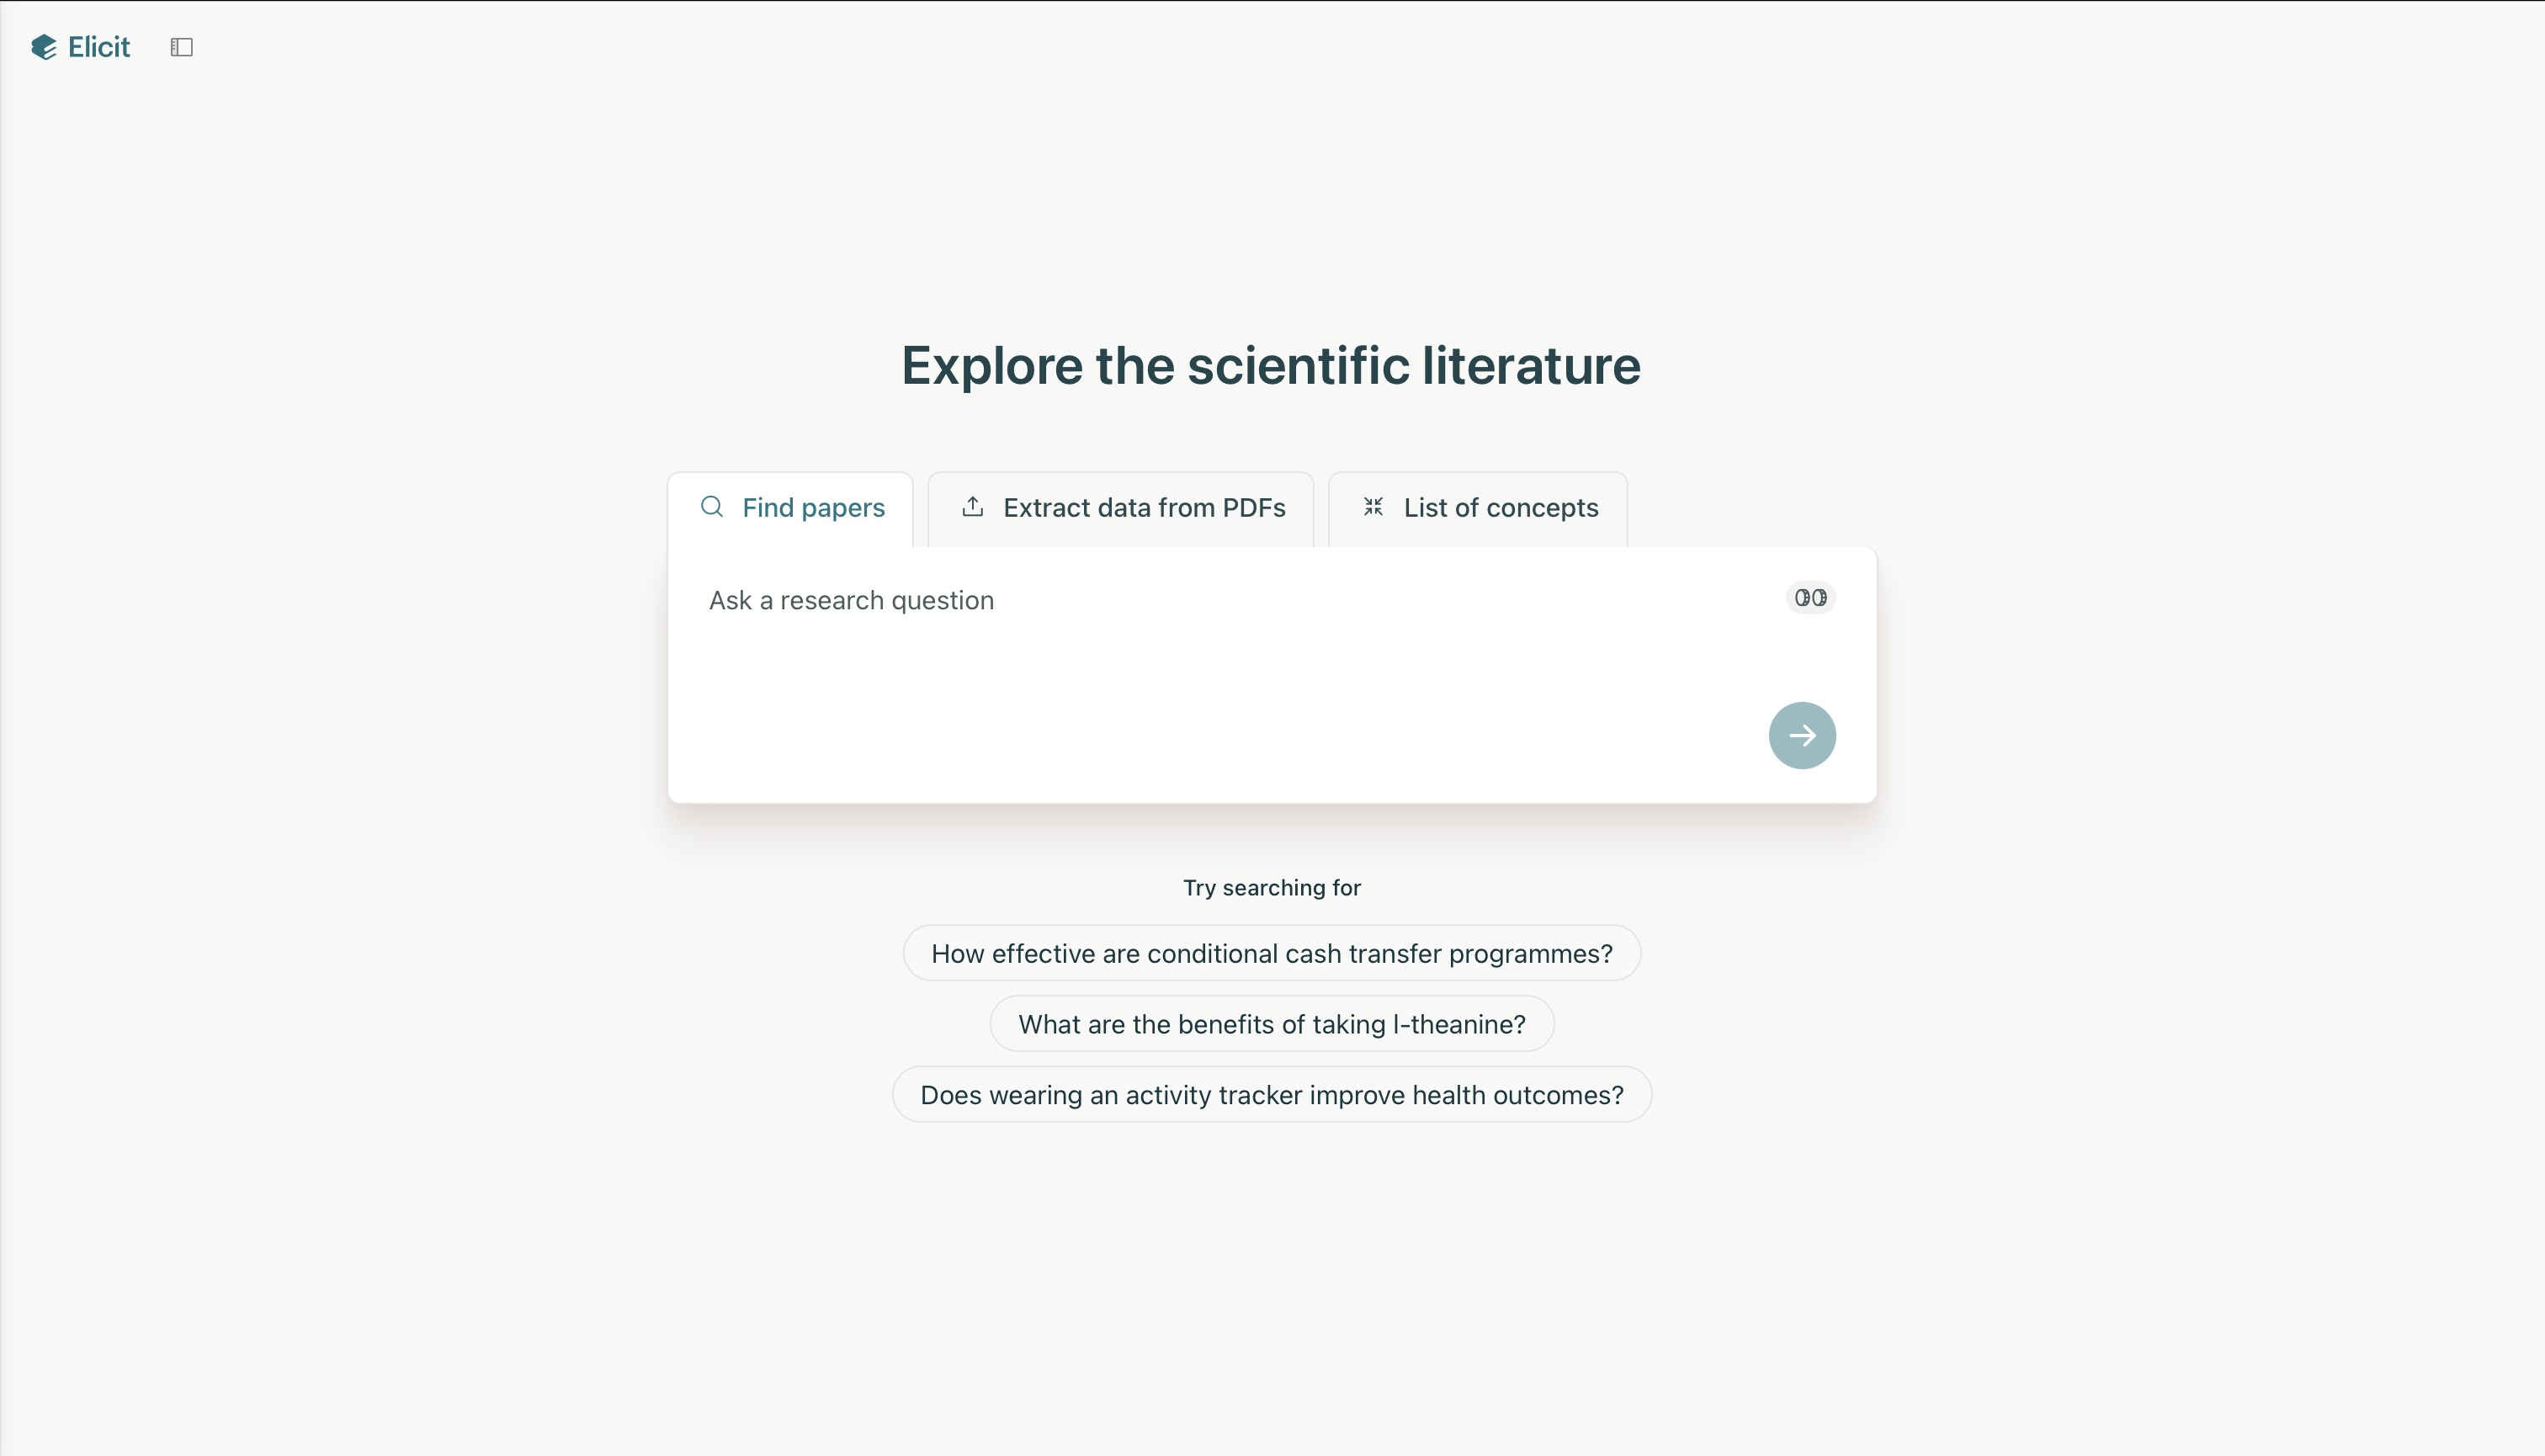
\includegraphics{images/chapitre9_image2.png}

}

\caption{\label{fig-elicit}Menu d'accueil d'Elicit}

\end{figure}%

Par exemple, disons que l'on s'intéresse à la question suivante:
qu'est-ce que la démocratie? Il peut être difficile de savoir par où
commencer face à l'impressionnant volume d'écrits sur le sujet.
\emph{Elicit} offre une solution à ce problème. La
Figure~\ref{fig-elicit} correspond au menu d'accueil du site web. Une
fois là, nous inscrivons la question qui nous intéresse dans la case «
\emph{Ask a research question} ». Les résultats générés sont représentés
dans la Figure~\ref{fig-results1} et Figure~\ref{fig-results2}

\begin{figure}

\centering{

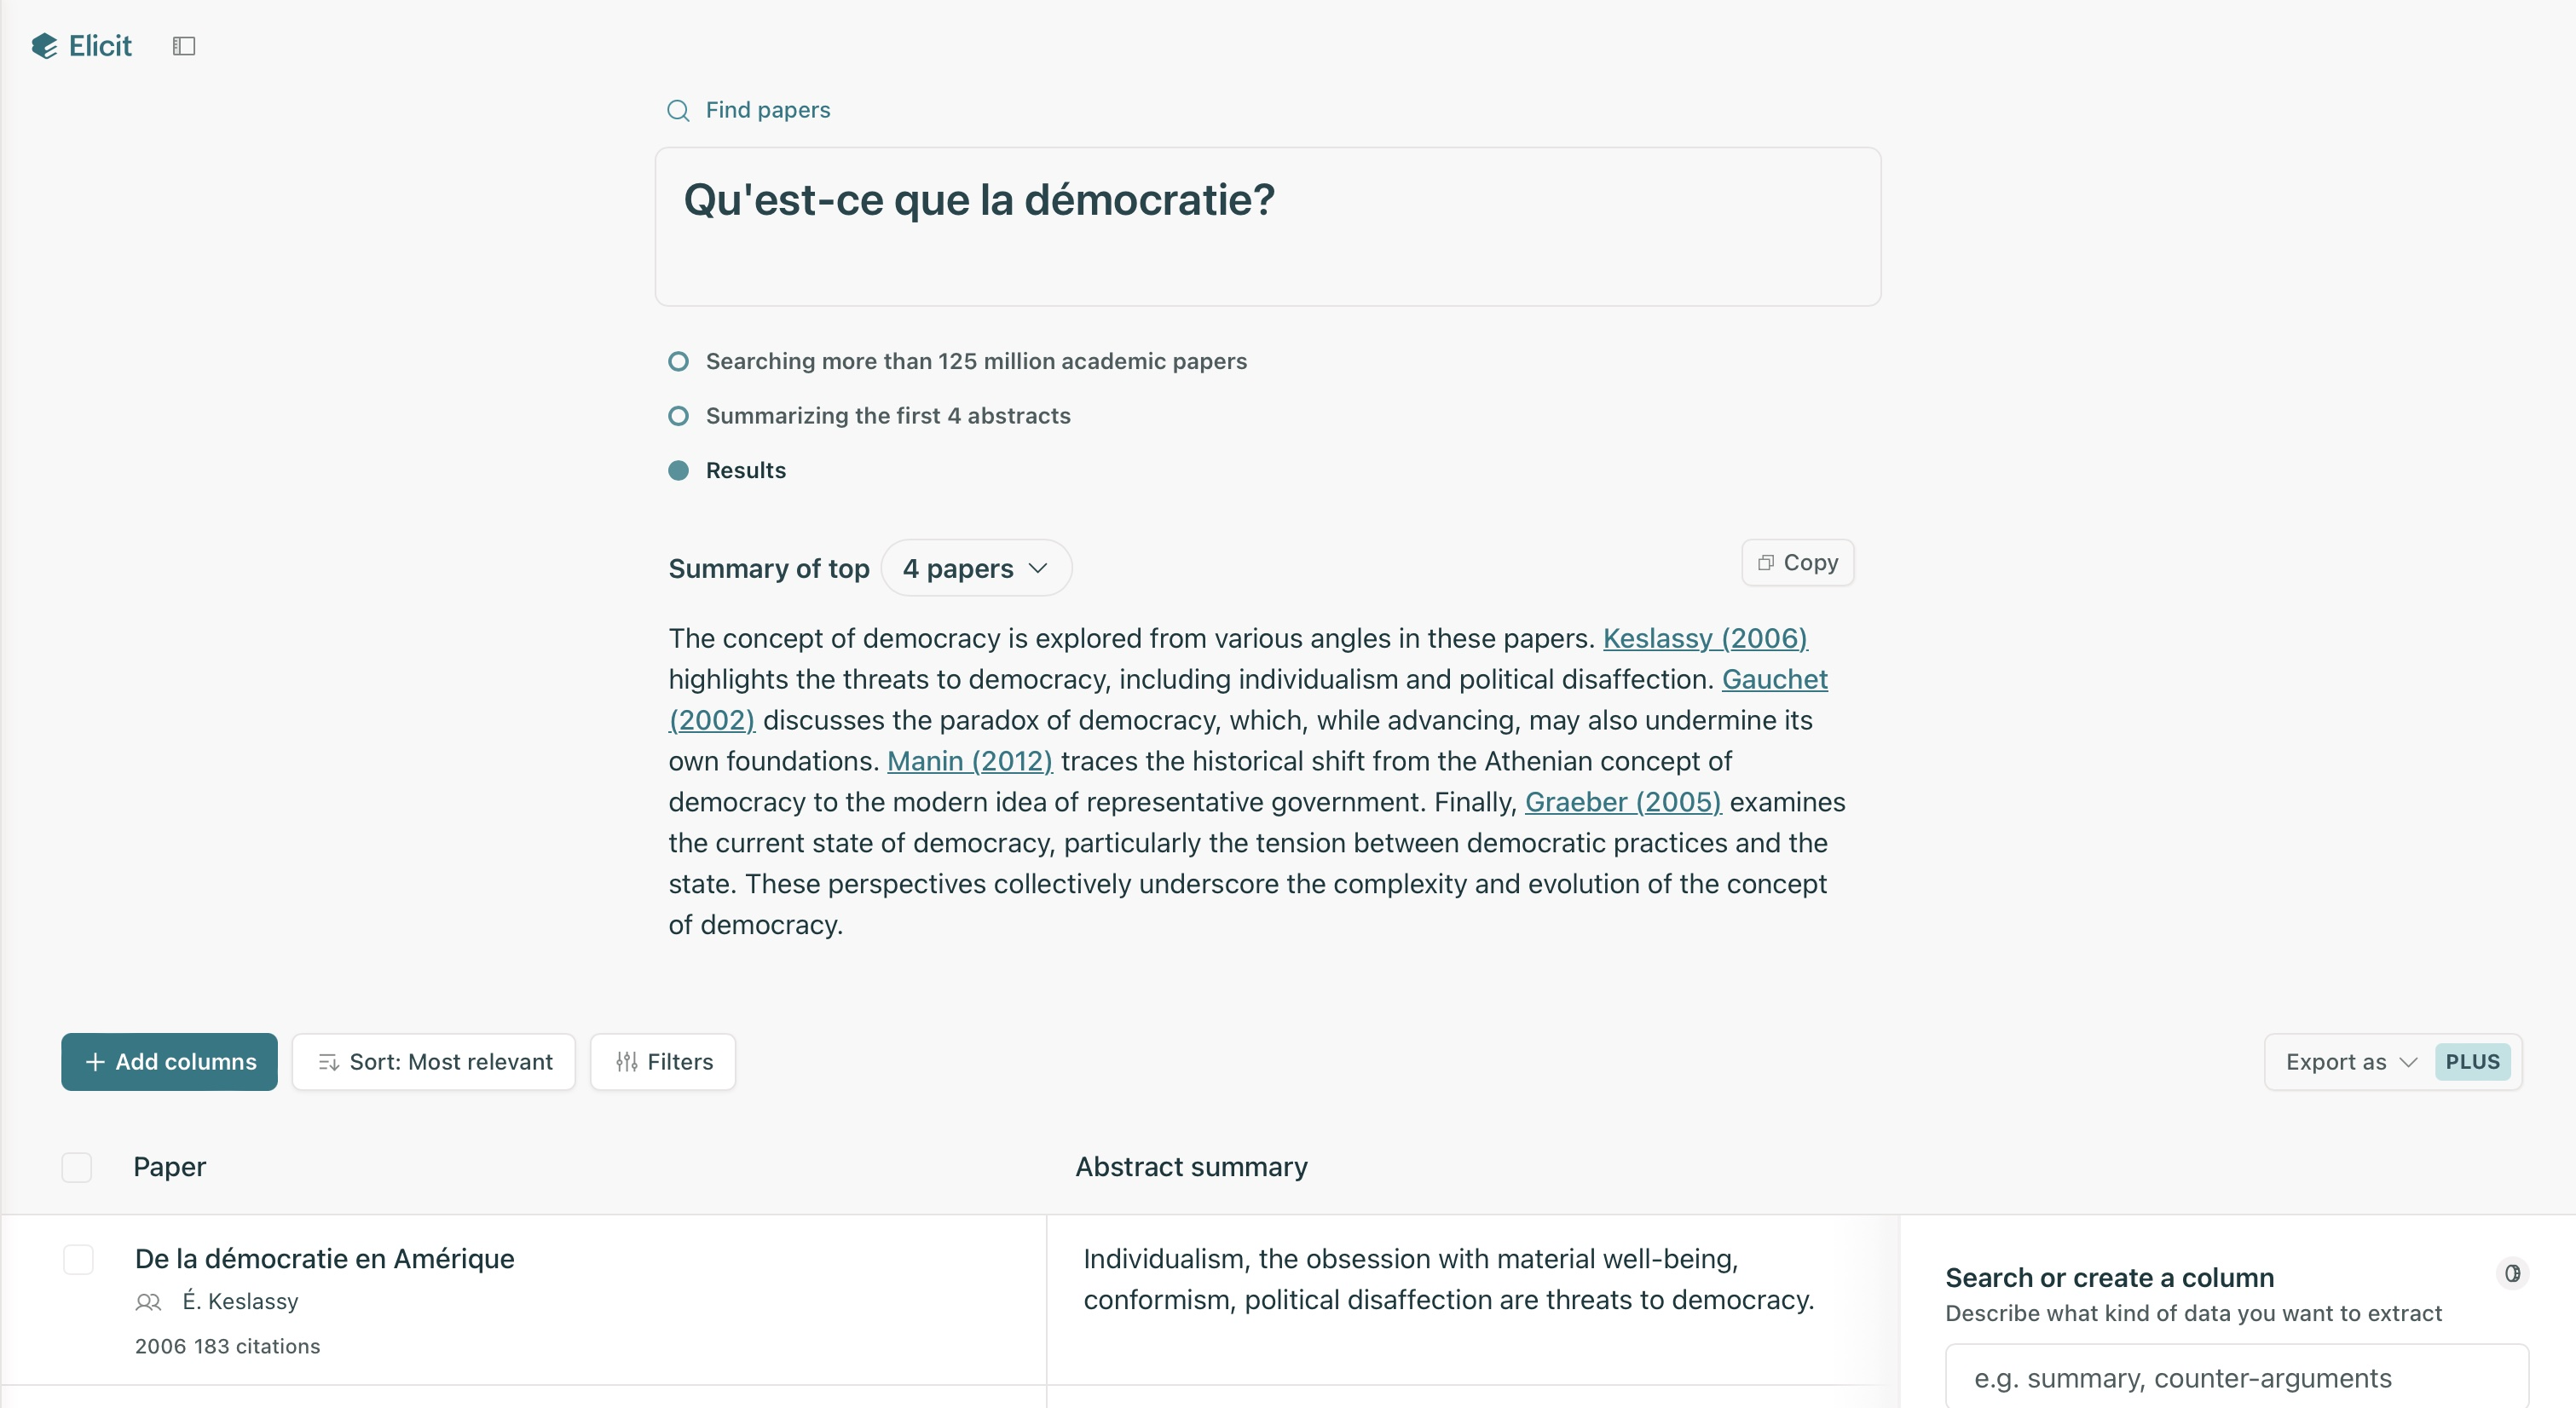
\includegraphics{images/chapitre9_image3.png}

}

\caption{\label{fig-results1}Court résumé du sujet}

\end{figure}%

\begin{figure}

\centering{

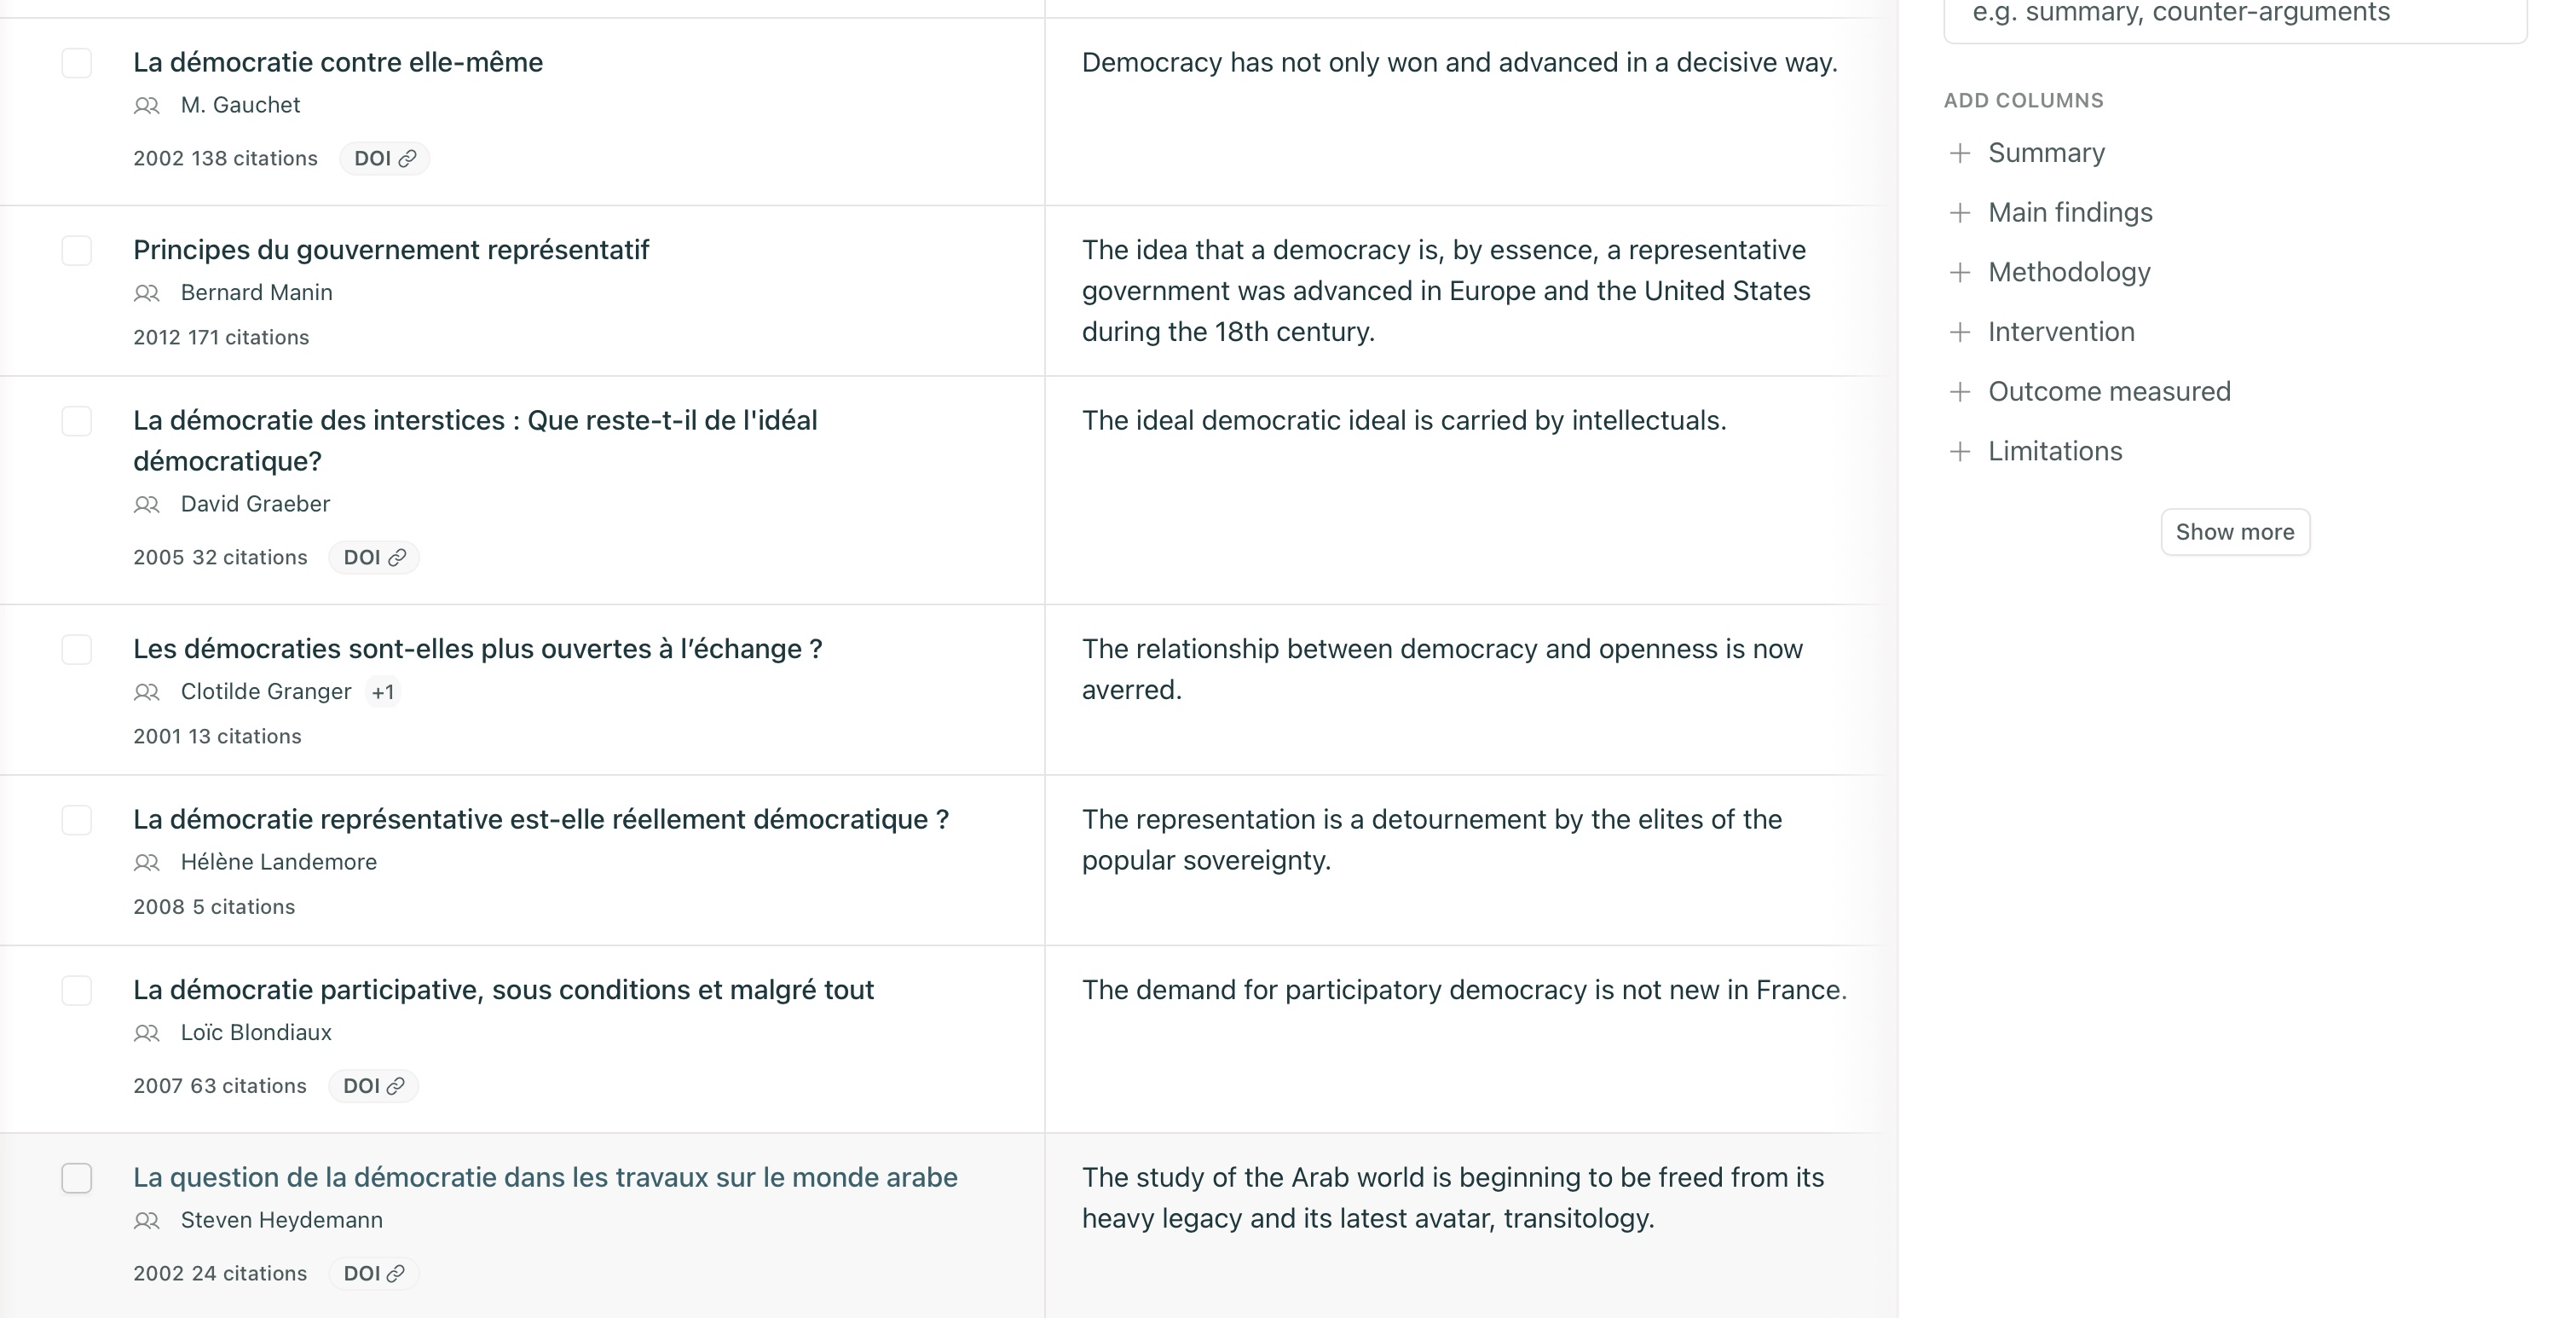
\includegraphics{images/chapitre9_image4.png}

}

\caption{\label{fig-results2}Suggestions de lectures}

\end{figure}%

Le logiciel offre donc un moyen intéressant afin de faire un premier «
filtrage » de la littérature sur un sujet, tout en fournissant un résumé
des sources suggérées à partir desquelles nous pouvons juger de sa
pertinence en fonction de nos besoins.

Cependant, il est fortement recommandé d'utiliser le résumé produit par
le logiciel, dans la Figure~\ref{fig-results1}, et ceux de chaque
suggestion, dans la Figure~\ref{fig-results2}, à titre indicatif et
uniquement pour notre propre réflexion. En d'autres termes, \textbf{ne
jamais faire un copier-coller de ces résumés afin de les inclure dans
notre travail de recherche}. Ce logiciel doit impérativement être
accompagné d'une utilisation intègre de la littérature. Une bonne
utilisation de ce logiciel devrait se limiter à trouver des articles
et/ou des livres scientifiques selon nos besoins qui seront consultés
par la suite pour rédiger notre revue des écrits et trouver des
références supplémentaires.

Un autre outil s'offre à nous afin de trouver des références
supplémentaires: \emph{ResearchRabbit}. Ce logiciel est gratuit, mais
demande de se créer un compte afin de pouvoir utiliser ses services. Une
fois que plusieurs articles et/ou chapitres de livre ont été lu, et
qu'ils ont été ajoutés dans Zotero, il est possible d'importer la
collection dans \emph{Research Rabbit}. La Figure~\ref{fig-rr1} présente
le menu principal du site web.

\begin{figure}

\centering{

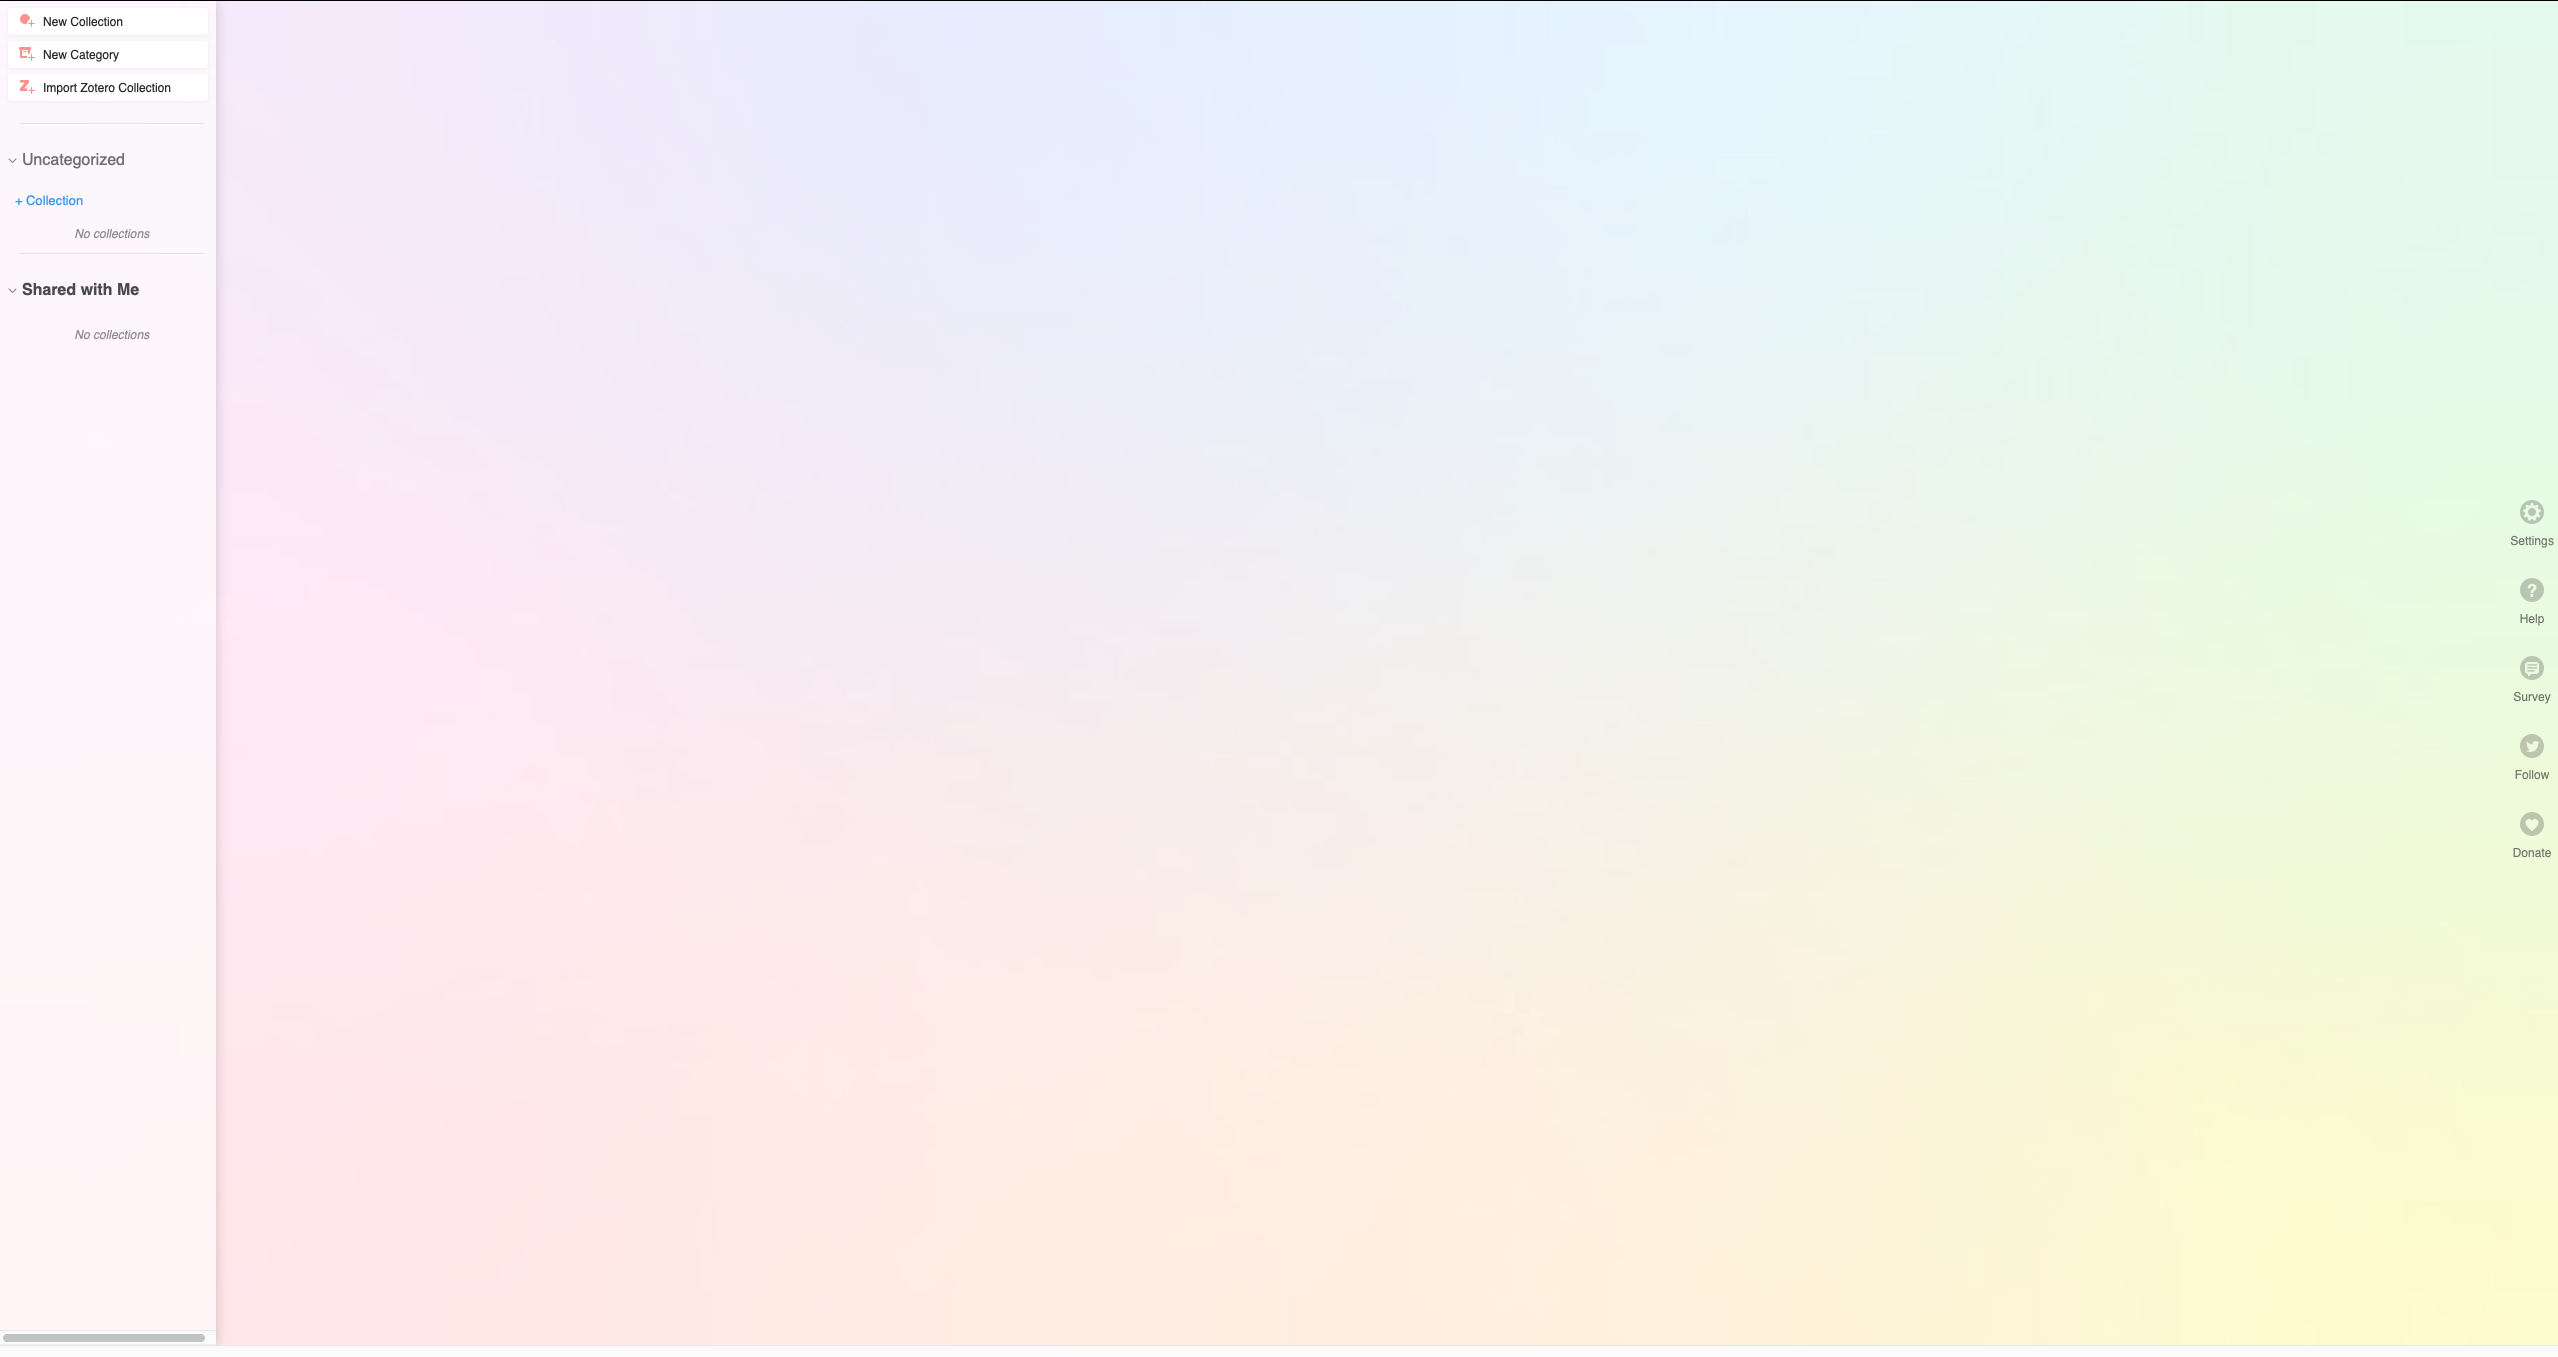
\includegraphics{images/chapitre9_RR1.png}

}

\caption{\label{fig-rr1}Menu principal}

\end{figure}%

\begin{figure}

\centering{

\includegraphics{images/chapitre9_rr2.png}

}

\caption{\label{fig-rr2}Importation manuelle de documents}

\end{figure}%

\begin{figure}

\centering{

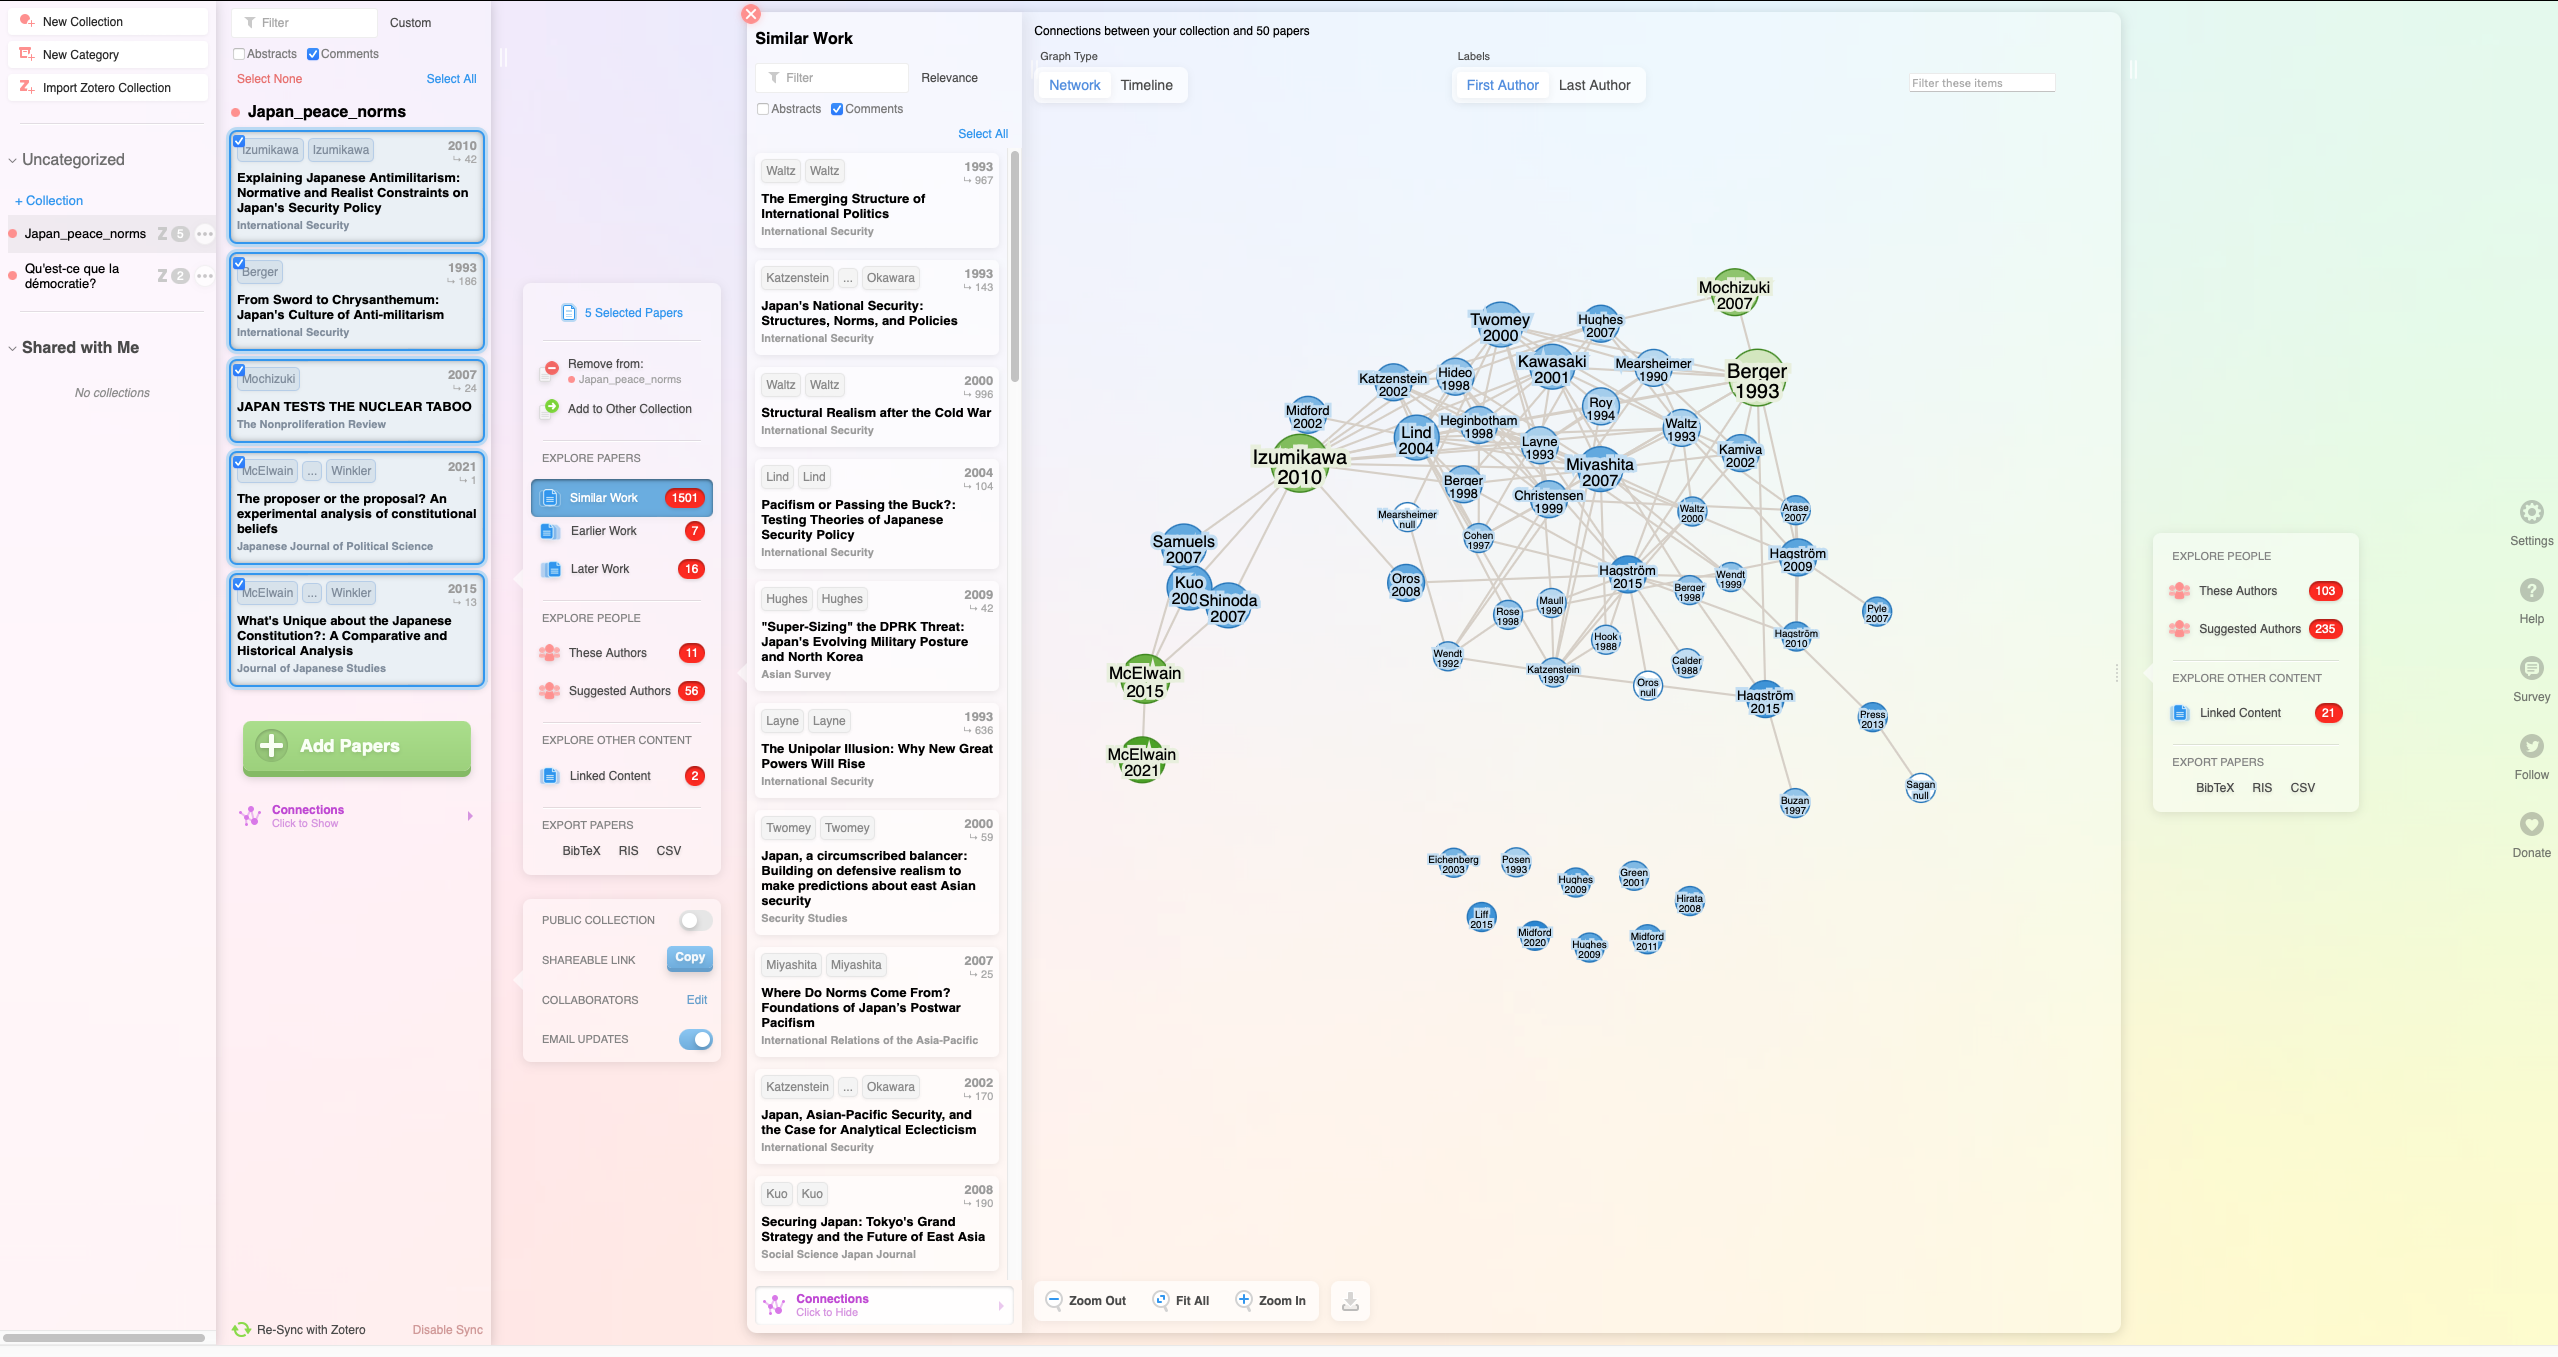
\includegraphics{images/chapitre9_RR3.png}

}

\caption{\label{fig-rr3}Présentation de la littérature similaire}

\end{figure}%

\begin{figure}

\centering{

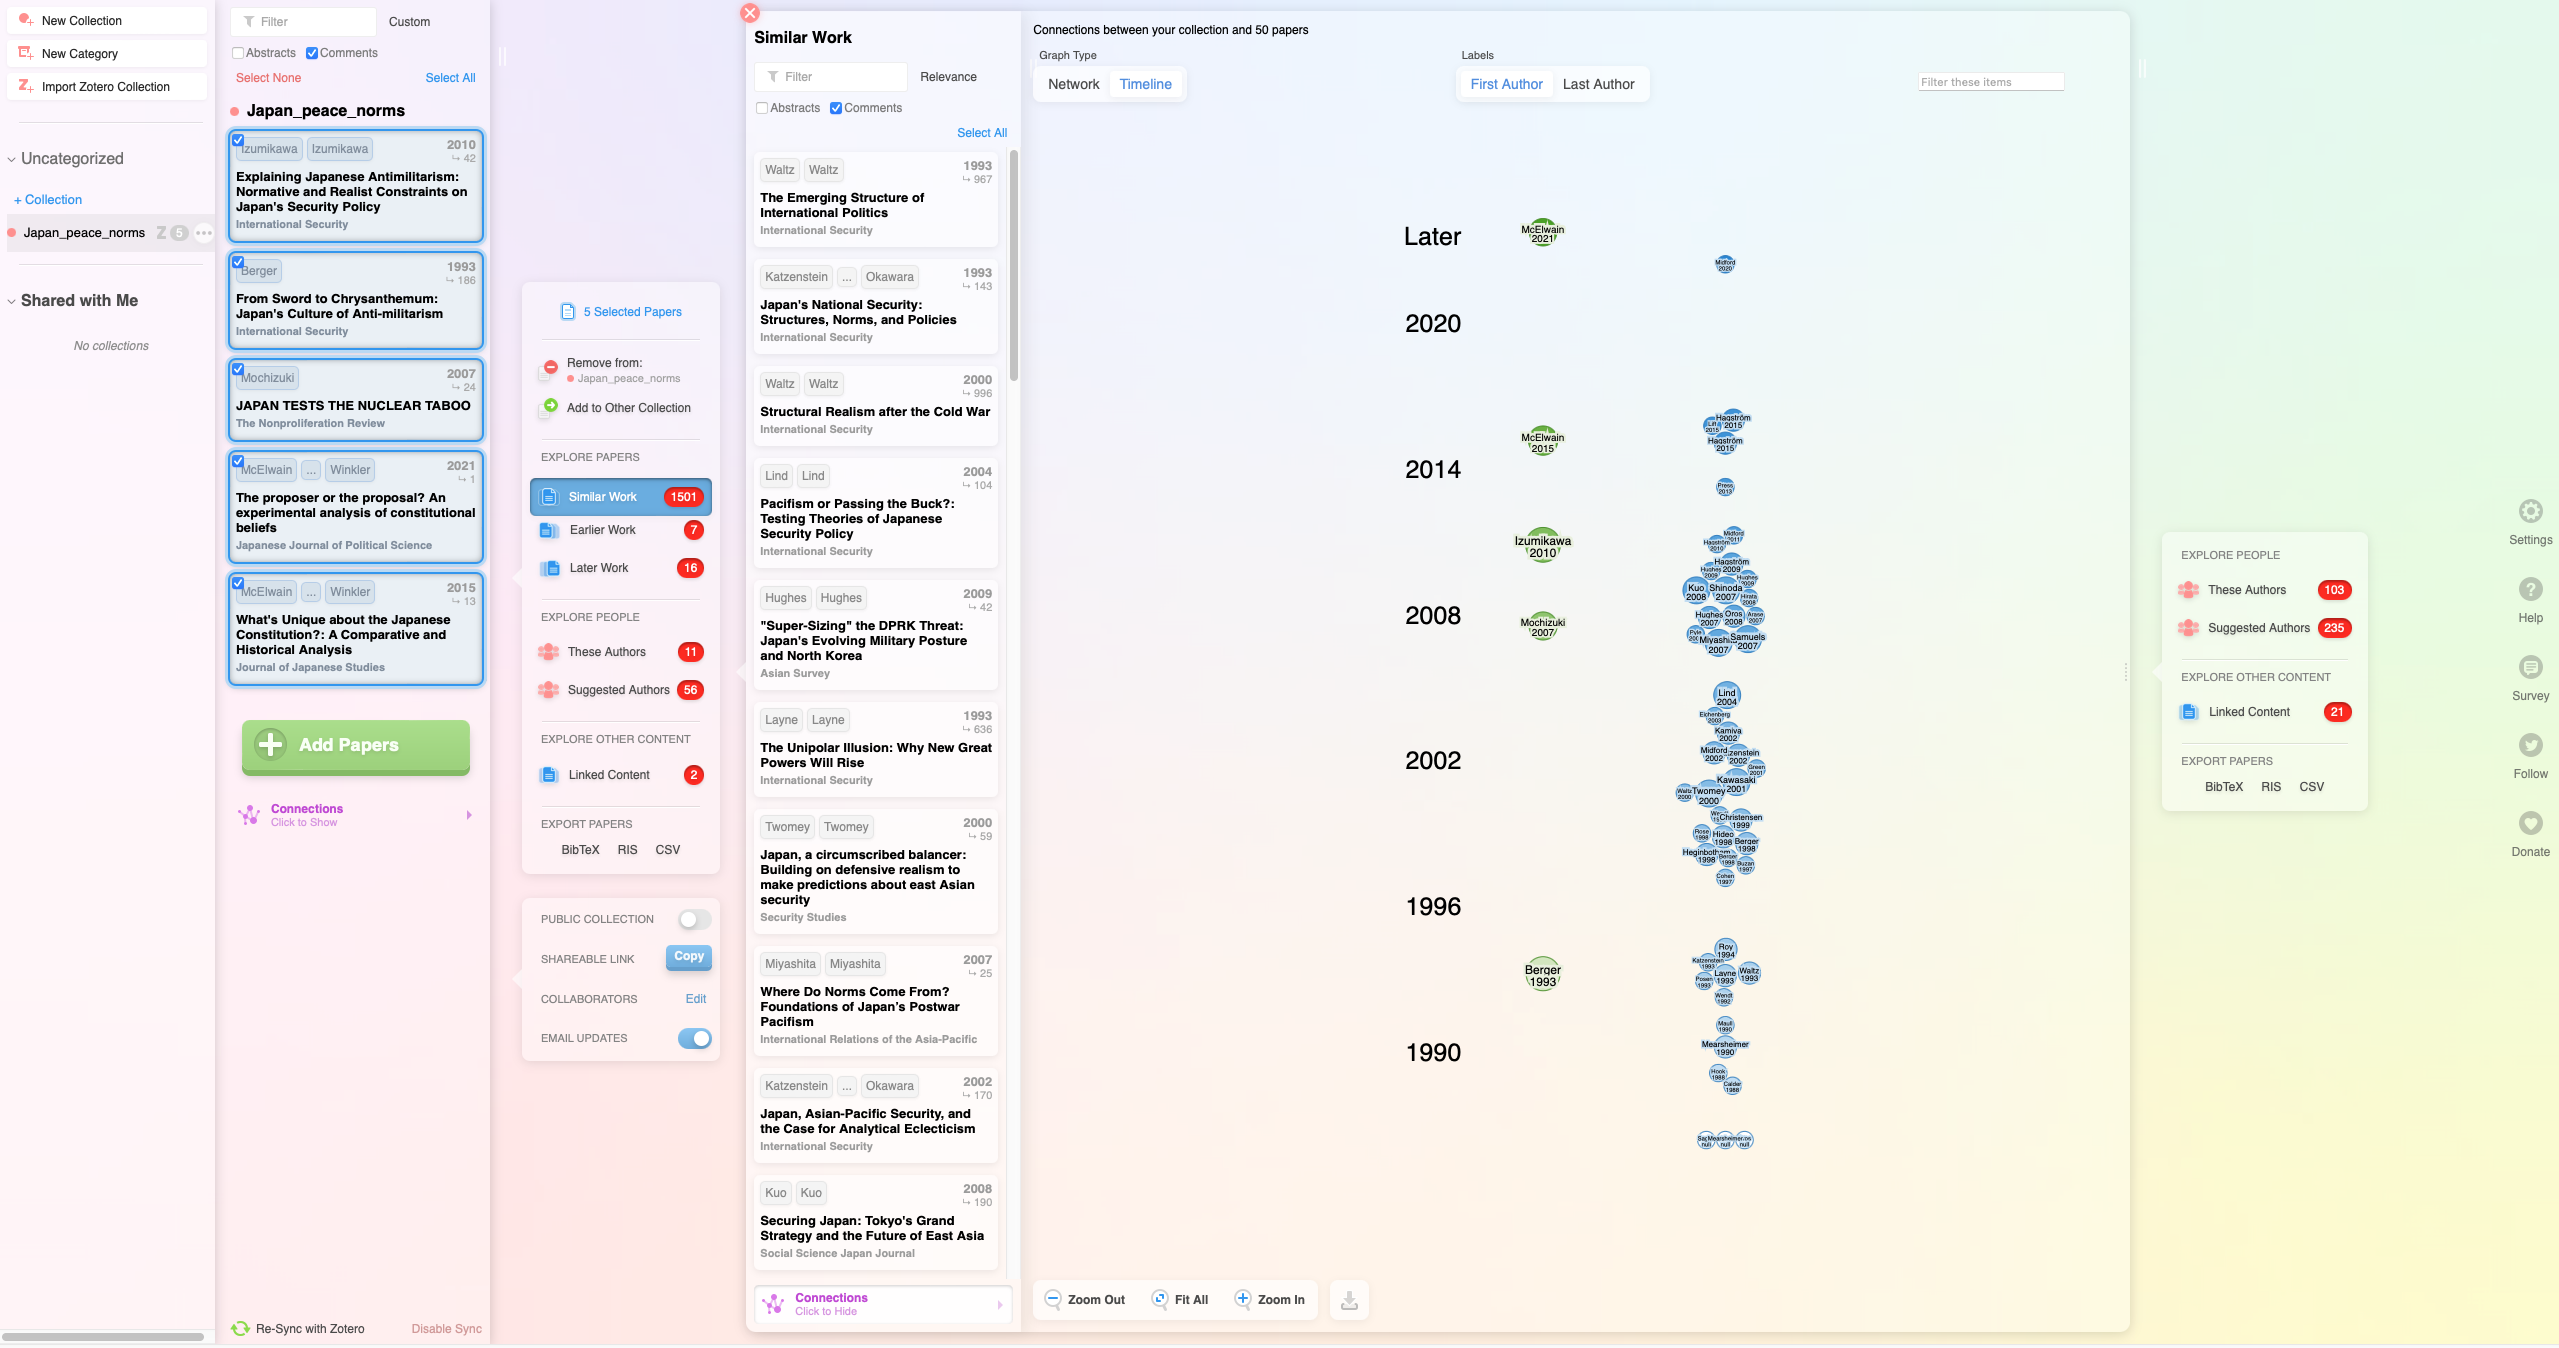
\includegraphics{images/chapitre9_rr4.png}

}

\caption{\label{fig-rr4}Vue « Timeline » des références}

\end{figure}%

Avant toute chose, \emph{Research Rabbit} doit être considéré comme un
outil qui aidera à \emph{complémenter} la revue des écrits. En d'autres
termes, afin que ce logiciel soit utile, il faut déjà avoir des articles
sous la main. \emph{Elicit} peut aider pour cette tâche, mais aussi il
est pratique de consulter des manuels de références comme des
\emph{hanbooks}\footnote{Il s'agit d'ouvrages généraux qui portent sur
  divers sujets. Les éditeurs les plus connus sont notamment
  \emph{Oxford}, \emph{SAGE} et \emph{Routledge}.} et autres ouvrages de
référence afin de se faire une idée sur le sujet qui nous intéresse en
plus de trouver des références. Au besoin, les bibliothécaires des
différents départements universitaires sont aussi d'excellente ressource
pour débuter une recherche.

Utilisons un exemple concret afin d'illustrer l'utilisation de
\emph{Research Rabbit}. Supposons que nous nous intéressons à la
question suivante : quel est le rôle des normes pacifistes sur les
processus politiques au Japon? Dans un premier temps, un survol rapide
de la littérature grâce aux ouvrages de références ainsi qu'avec Google
Scholar a permis d'identifier quelques textes qui sont jugés comme
pertinents afin de fournir une réponse à cette question. Ceux-ci sont
ensuite ajouté dans une nouvelle collection Zotero\footnote{Voir le
  Chapitre~\ref{sec-chap4} au besoin.}, qui contiendra uniquement les
ouvrages pour ce projet. Ce dernier point est important afin d'éviter
d'ajouter du « bruit » dans les suggestions de \emph{Research Rabbit}.
Une fois ces étapes faites, il est possible d'importer la collection
dans \emph{Research Rabbit}. Pour ce faire, il faut cliquer sur le
bouton \emph{Import Zotero Collection}, situé dans le coin supérieur
gauche de la Figure~\ref{fig-rr1}.

Il se peut que le logiciel ne trouve pas tous les articles qui se
trouvent dans la collection Zotero. Une solution, lorsque ce problème
arrive, est de cliquer sur le bouton vert \emph{Add Paper} situé dans la
colonne de notre collection. La Figure~\ref{fig-rr2} montre la barre de
recherche qui apparaitra, et dans laquelle il est possible d'ajouter
manuellement les articles au besoin. Une fois que les références ont été
ajoutées, \emph{Research Rabbit} pourra dresser une « cartographie » des
différentes sources qui sont en lien avec ces articles. La
Figure~\ref{fig-rr3} présente cette cartographie.

Il est possible de trouver des articles supplémentaires à l'aide de
trois fonctionnalités. La première est de consulter les \emph{Similar
Work}. Cette option est intéressante afin de visualiser tous les
articles qui sont similaires aux ouvrages qui ont été identifiés au tout
début. Les points en vert sont les sources qui font partie de ma
collection. Cependant, la visualisation offerte par cette option peut
rapidement devenir chargée. Comme la Figure~\ref{fig-rr3} l'illustre, en
fonction des cinq articles que j'ai importés dans Zotero, il y a 1 501
articles similaires. Cela complique la tâche de ciblage. Ainsi, la
deuxième option est d'utiliser \emph{Earlier Work} et \emph{Later Work},
surtout avec la vue \emph{Timeline} comme dans la Figure~\ref{fig-rr4}.
Il est toujours utile de classifier les ouvrages en fonction de leur
date de parution, notamment afin de suivre l'évolution du débat
scientifique à propos du sujet de notre recherche. Cette fonctionnalité
de \emph{Research Rabbit} facilite ainsi cette étape, en plus de
permettre de découvrir des ouvrages qui ont été publiés avant et aprés
ceux qui ont été préalablement identifié.

Une troisième option est de sélectionner une seule source à la fois, et
de consulter les deux options suivantes : \emph{All References} et
\emph{All Citations}. Elles permettent, respectivement, de visualiser
tous les articles qui sont cités dans l'article selectionné, et de
visualiser les travaux qui ont cité l'article en question. Ces options
sont donc très utiles pour passer au « peigne fin » chacun des articles
afin de dénicher des sources supplémentaires selon la méthode « boule de
neige ». Cependant, il faut faire attention dans l'utilisation de cette
méthode. Il y a un risque « d'effet tunnel », soit que la revue des
écrits qui sera faite à partir de ces sources manque de largeur et de
représentativité dans le traitement du sujet. C'est pourquoi il est
important de diversifier ces sources et d'utiliser ces deux options
d'une façon complémentaire avec plusieurs articles différents. Il est
donc utile d'ajouter au fur et à mesure les nouvelles références dans
\emph{Research Rabbit} afin de visualiser la couverture de notre revue
des écrits.

\subsection{Pendant la recherche: l'utilisation de grands modèles
linguistiques}\label{pendant-la-recherche-lutilisation-de-grands-moduxe8les-linguistiques}

pour analyser des données

L'utilisation des LLMs via l'API d'OpenAI en R représente une avancée
significative pour les chercheurs en sciences sociales, leur offrant des
outils puissants pour naviguer et analyser l'immense paysage des données
textuelles avec une précision et une efficacité accrues.

Bien qu'il soit possible de communiquer avec l'API d'OpenAI directement,
le package \texttt{openai} en R offre une interface conviviale pour
interagir avec les modèles de langage, permettant aux chercheurs de
tirer parti de ces outils avancés sans nécessiter une expertise en
informatique ou en apprentissage automatique. Le package fournit des
fonctions pour générer du texte, analyser des sentiments, extraire des
entités, et biens plus encore, facilitant l'intégration des LLMs dans le
flux de travail des recherches existantes.

OpenAi (2019) définit les grands modèles linguistiques (Large language
models ou LLMs en anglais) comme des modèles d'apprentissage automatique
de grande échelle, formés pour prédire le mot suivant dans un texte en
se basant sur les mots précédents. Ils sont entraînés sur de vastes
quantités de données textuelles, telles que des articles de journaux,
des livres, des pages Web, des courriels, des messages de médias
sociaux. Cette méthode d'entraînement simple permet aux modèles de
démontrer naturellement des compétences dans de nombreuses tâches et
domaines divers, sans nécessiter de formation spécifique à la tâche. Il
est important de noter qu'ils ne sont que des algorithmes de prédiction
textuelle et ne possèdent pas la faculté de réfléchir ou de comprendre.

L'intégration des grands modèles de langage via l'API d'OpenAI dans la
recherche en sciences sociales numériques ouvre des horizons prometteurs
pour l'analyse qualitative et quantitative des données textuelles.
L'utilisation de ces modèles en R permet aux chercheurs d'exploiter des
capacités avancées de traitement du langage naturel pour une variété
d'applications allant de la simple extraction de données à des analyses
complexes de contenu et de sentiment. Elle permet aussi de générer des
données pour l'analyse de biais algorithmiques en comparant
l'information générée par les modèles avec des données de référence
générées par des humains. Les LLMs peuvent être utilisés pour l'analyse
de sentiments, l'extraction d'entités et de relations, la génération de
résumés de texte, la simulation de dialogue, la traduction et la
localisation, et le développement d'outils personnalisés pour des
besoins spécifiques de recherche.

Voici quelques exemples d'utilisation des LLMs en sciences sociales.
Pour des cas concrets d'application, voir la section « L'IA en sciences
sociales » dans ce chapitre.

\begin{enumerate}
\def\labelenumi{\arabic{enumi}.}
\item
  Premièrement, les LLMs peuvent être utilisés pour l'analyse de
  sentiments, permettant aux chercheurs de détecter des nuances dans les
  opinions exprimées dans des corpus de données volumineux, tels que des
  commentaires sur les réseaux sociaux, des critiques de produits, ou
  des discours politiques. Cette analyse peut révéler des tendances de
  sentiment général ou être segmentée pour examiner des variations entre
  différents groupes démographiques ou chronologiques.
\item
  Deuxièmement, les LLMs offrent des capacités d'extraction d'entités et
  de relation, ce qui est crucial pour structurer des données non
  structurées comme des questions de sondage ouvertes. Les chercheurs
  peuvent extraire des personnes, des lieux, des institutions, et même
  des concepts ou des événements, liant ces entités à des thèmes
  spécifiques ou à des contextes historiques et sociopolitiques,
  enrichissant ainsi les bases de données pour des études plus poussées.
\item
  Troisièmement, la génération automatique de résumés de textes par ces
  modèles permet de condenser de grandes quantités d'informations en
  résumés concis, facilitant l'analyse préliminaire de vastes archives
  de textes, comme des articles de presse, des mémoires juridiques, ou
  des écrits académiques. Cela aide les chercheurs à identifier
  rapidement les documents pertinents sans nécessiter la lecture
  intégrale des textes.
\item
  Quatrièmement, les modèles linguistiques peuvent être utilisés pour
  générer des simulations de dialogue ou des réponses à des questions
  hypothétiques, permettant aux chercheurs en sciences sociales de
  modéliser des interactions entre différents acteurs sociaux ou
  d'explorer des scénarios hypothétiques en études de comportement sans
  la mise en place de coûteuses études de terrain.
\item
  Cinquièmement, l'intégration de LLMs aide à surmonter les barrières
  linguistiques dans la recherche globale, en offrant des capacités de
  traduction et de localisation qui permettent une analyse plus
  inclusive des textes dans différentes langues, essentielle pour les
  études comparatives internationales.
\item
  Sixièmement, les modèles de ``speech-to-text'' peuvent être utilisés
  pour transcrire automatiquement des enregistrements audio en texte,
  comme des entrevues, facilitant l'analyse de discours oraux ou de
  conversations enregistrées, et permettant aux chercheurs de travailler
  avec des données multimodales pour des études interdisciplinaires.
\item
  Septièmement, les modèles de vision algorithmiques permettent
  l'analyse de contenu visuel, en extrayant des informations à partir
  d'images ou de vidéos pour compléter des analyses textuelles, ou pour
  étudier des phénomènes visuels comme la représentation des genres dans
  les médias ou les tendances de la mode.
\item
  Enfin, les chercheurs peuvent utiliser les LLMs pour développer des
  outils personnalisés qui s'adaptent à des besoins spécifiques de
  recherche, comme l'analyse de discours ou la détection de changements
  dans le langage au fil du temps, fournissant ainsi des informations
  précieuses sur l'évolution des discours et pratiques culturelles.
\end{enumerate}

Voici un exemple simple d'utilisation de l'API d'OpenAI :

\begin{Shaded}
\begin{Highlighting}[]

\FunctionTok{library}\NormalTok{(openai)}

\NormalTok{system }\OtherTok{\textless{}{-}} \StringTok{"You are a helpful assistant"} \CommentTok{\# Donne un role au modèle.}
\NormalTok{Doit être clair et concis}

\NormalTok{prompt }\OtherTok{\textless{}{-}} \StringTok{"Quelle est la capitale du Québec?"} \CommentTok{\# Le prompt}

\NormalTok{chat\_prompt }\OtherTok{\textless{}{-}}\NormalTok{ openai}\SpecialCharTok{::}\FunctionTok{create\_chat\_completion}\NormalTok{(}
    \AttributeTok{model =} \StringTok{"gpt{-}3.5{-}turbo{-}0125"}\NormalTok{, }\AttributeTok{messages =} \FunctionTok{list}\NormalTok{(}
        \FunctionTok{list}\NormalTok{(}\StringTok{"role"} \OtherTok{=} \StringTok{"system"}\NormalTok{,}
         \StringTok{"content"} \OtherTok{=}\NormalTok{ system}
\NormalTok{        ), }\FunctionTok{list}\NormalTok{(}
        \StringTok{"role"} \OtherTok{=} \StringTok{"user"}\NormalTok{, }\StringTok{"content"} \OtherTok{=}\NormalTok{ prompt)}
\NormalTok{        )}
\NormalTok{    )}

\NormalTok{output }\OtherTok{\textless{}{-}}\NormalTok{ chat\_prompt}\SpecialCharTok{$}\NormalTok{choices}\SpecialCharTok{$}\NormalTok{message.content}

\FunctionTok{print}\NormalTok{(output)}
\end{Highlighting}
\end{Shaded}

\subsection{Après la recherche: traduire ses écrits pour la
diffusion}\label{apruxe8s-la-recherche-traduire-ses-uxe9crits-pour-la-diffusion}

L'IA a aussi permis la création de nouveaux outils de traduction
automatique (\emph{machine translation}). Pris au sens large, le concept
de traduction automatique englobe n'importe quelle tâche de traduction
qui est réalisée par un algorithme, une machine ou des ordinateurs. sans
aucune aide d'un humain (Glover, 2024; Tabsharani, 2023). Il existe
différentes approches de traduction automatique:

\begin{enumerate}
\def\labelenumi{\arabic{enumi}.}
\tightlist
\item
  Basée sur des règles (\emph{rules-based}): utilise des règles
  linguistiques et des dictionnaires pour transformer les mots et
  phrases d'une langue source en langue cible. Nécessite des experts
  pour créer et maintenir ces règles, ce qui rend le processus
  laborieux, mais efficace pour les langues à grammaire bien définie.
\item
  Statistique (\emph{statistical}): analyse de grands volumes de textes
  bilingues pour identifier des motifs et probabilités. Utilise des
  modèles statistiques plutôt que des règles linguistiques pour
  déterminer les traductions les plus probables à partir des données
  d'apprentissage. Fonctionne bien avec des données volumineuses, mais
  peut parfois produire des traductions imprécises faute de
  contextualisation. 3. Basée sur des exemples (\emph{example-based}) :
  repose sur une base de données de phrases ou de segments précédemment
  traduits pour générer des traductions, en recherchant des exemples
  similaires dans la base de données et en récupérant les traductions
  les plus pertinentes, ce qui est utile pour des domaines spécifiques
  ou des textes très répétitifs, mais peut être limité face à des usages
  linguistiques nouveaux ou créatifs. 4. Neuronale (\emph{neural}) :
  utilise des modèles d'apprentissage profond pour apprendre les schémas
  de traduction, traitant des phrases entières et leur contexte, ce qui
  améliore la qualité et la fluidité des traductions, bien qu'elle ne
  remplace pas entièrement les traducteurs humains. 5. Hybride : les
  quatres approches peuvent également être combinées.
\end{enumerate}

C'est au sein de l'approche neuronale que les avancées en intelligence
artificielle ont permis de développer de nouveaux outils de traduction
automatique. En effet, les réseaux neuronaux transformeurs
(\emph{transformer neural networks}) ont révolutionné le domaine de la
traduction automatique en traitant des phrases entières dans leur
contexte global plutôt que des mots isolés, ce qui a considérablement
amélioré la qualité et la fluidité des traductions (Glover, 2024;
Tabsharani, 2023). En tant que forme d'IA générative, ces outils
exploitent le traitement du langage naturel (\emph{natural language
processing}), l'apprentissage profond (\emph{deep learning}) et
l'auto-attention (\emph{self-attention}) pour réaliser ces avancées. Ces
outils de traduction automatique sont devenus de plus en plus populaires
et accessibles, permettant à des personnes de traduire des textes
entiers, des sites Web, des documents, en quelques secondes, sans avoir
besoin de connaître la langue cible.

Il est très utile pour les chercheurs en sciences sociales numériques de
connaître et d'utiliser les outils de traduction automatique, car ils
facilitent la recherche, la communication et la collaboration à
l'échelle internationale, particulièrement dans le contexte d'un monde
académique dominé par l'anglais. Toutefois, il est crucial de comprendre
que ces outils ne remplacent pas complètement les traducteurs humains.
Voici, d'une perspective générique, les avantages et inconvénients de
ces outils par rapport à la traduction humaine (Glover, 2024):

\begin{longtable}[]{@{}
  >{\raggedright\arraybackslash}p{(\columnwidth - 2\tabcolsep) * \real{0.4306}}
  >{\raggedright\arraybackslash}p{(\columnwidth - 2\tabcolsep) * \real{0.5694}}@{}}
\toprule\noalign{}
\begin{minipage}[b]{\linewidth}\raggedright
Avantages
\end{minipage} & \begin{minipage}[b]{\linewidth}\raggedright
Inconvénients
\end{minipage} \\
\midrule\noalign{}
\endhead
\bottomrule\noalign{}
\endlastfoot
Amélioration de la productivité : traductions rapides et de grande & \\
échelle & Données biaisées : reproduction de stéréotypes et erreurs \\
de genre & \\
à l'apprentissage non supervisé & Manque de subtilité : difficultés \\
avec les expressions idiomatiques et le jargon spécifique & \\
Réduction des coûts : minimise le besoin d'intervention humaine & \\
\end{longtable}

Difficultés avec le contexte : erreurs de cohérence et de pertinence
contextuelle \textbar{} \textbar{} Amélioration de l'accessibilité :
accessible en plusieurs langues et adapté aux besoins spéciaux
\textbar{} \textbar{}

Il existe des milliers d'outils de traduction automatique qui utilisent
l'IA d'une façon ou d'une autre. Dans les prochaines pages, nous
présenterons rapidement quelques-uns de ces outils gratuits parmi les
plus populaires actuellement en mettant en lumière leurs forces et leurs
faiblesses. Il est important de noter que ces outils sont en constante
évolution et que leur qualité peut varier en fonction de la langue, du
contexte et du type de texte à traduire. Par ailleurs, bien qu'ils ne
relèvent pas de l'intelligence artificielle, des ressources comme
\emph{TERMIUM Plus} et \emph{Interactive Terminology for Europe (IATE)}
jouent un rôle complémentaire essentiel dans le travail de
traduction\footnote{L'épistémologie est l'une des branches de la
  philosophie des sciences qui s'intéresse au savoir et à la
  connaissance. De manière générale, et très simplifié, l'une des
  questions fondamentales de l'épistémologie et de se questionner quant
  à savoir ce qu'est un savoir qui serait scientifique.}.

\subsubsection{Google Traduction}\label{google-traduction}

Très connue, l'une des forces de Google Traduction est son support d'une
large variété de langues, tant des langues globalement utilisées et des
langues plus régionales et moins utilisées. Google Traduction est basé
sur de la traduction automatique neuronale, prenant donc le sens et le
contexte d'une phrase en considération. De plus, il supporte aussi la
traduction de documents complets.

\subsubsection{DeepL}\label{deepl}

DeepL se démarque par une qualité supérieure de traduction, mais dans un
nombre de langues plus restreint que d'autres outils. Il est aussi basé
sur de la traduction automatique neuronale, ce qui lui permet de prendre
en compte le contexte et la complexité d'une structure de phrase.

\subsubsection{Mate Translate}\label{mate-translate}

Mate Translate est une extension de navigateur qui permet de traduire
des pages web entières, des phrases ou des mots en un seul clic. Il
supporte un grand nombre de langues et offre des fonctionnalités
supplémentaires telles que la prononciation des mots et des phrases
traduits. Son avantage réside vraiment dans sa facilité d'utilisation et
sa rapidité.

\subsubsection{ChatGPT}\label{chatgpt}

Évidemment, ChatGPT est un outil de traduction automatique basé sur des
modèles de langage génératif. Il est très populaire pour sa capacité à
générer du texte de manière fluide et naturelle, ce qui en fait un outil
de traduction très efficace pour les textes longs et complexes. De plus,
il est possible de raffiner la traduction en quelques itérations en
suggérant des modifications au texte traduit.

\subsubsection{Autres outils}\label{autres-outils}

Comme mentionné plus haut, il existe une panoplie d'outils de traduction
automatique qui utilisent l'IA et qui sont accessibles gratuitement.
Cependant, considérant que ces outils sont en constante évolution,
l'objectif de ce livre n'est pas d'en faire une description exhaustive,
mais plutôt de donner un aperçu des possibilités offertes par ces
outils. Parmi les autres outils populaires, on peut citer Microsoft
Translator, Pairaphrase, Amazon Translate, Smartling, Unbabel, Linguee,
Yandex.Translate, HIX Translate, etc.

\section{Quelle est la place du chercheur
maintenant?}\label{quelle-est-la-place-du-chercheur-maintenant}

Avec l'avènement de l'IA, il est tout à fait raisonnable de se demander
quelle est la place du chercheur aujourd'hui. L'avenir du chercheur
est-il en danger? Pourrait-on assister au développement des sciences
sociales sans chercheur humain derrière? Si tel est le cas, est-ce que
ça ne constituerait pas un paradoxe important? Est-ce que la machine est
mieux placée pour comprendre la réalité du monde sociale, ainsi que ses
mécanismes, que l'humain? D'une part, certains pensent que l'IA risque
de générer des « laboratoires autonomes » (Hanchen Wang, Tianfan Fu,
Yuanqi Du, Wenhao Gao, Kexin Huang, et al., 2023, pp.~55). Il n'est pas
difficile d'imaginer un monde où tout le processus scientifique, de la
conception jusqu'à la communication, serait fait par l'IA. Le chercheur
perdrait ainsi sa profession, et se limiterait à n'être qu'une partie de
l'auditoire vers qui les résultats sont présentés.

Bien que nous n'en sommes pas encore là, il est important de réfléchir
aux différents enjeux qui se posent à l'aube d'une révolution
technologique. Par exemple, étant donné que l'IA est, pour l'instant,
très opaque dans tout le processus qui le mène de l'intrant vers le
résultat, comment pourrait-on s'assurer que la machine a pris toutes les
précautions nécessaires pour respecter les différents enjeux éthiques?
A-t-elle eu le consentement libre et éclairé de tous les participants?
De plus, quel est le niveau de confiance que nous pouvons avoir envers
des résultats dont on ne connait pas le processus qui y a mené? Sur
cette dernière question, l'une des caractéristiques fondamentales de la
science est la reproductibilité des protocoles scientifiques (Bourgeois,
2021; King et al., 2021). Toutes les recherches doivent présenter, d'une
manière très précise, comment les données ont été choisies, comment
elles ont été collectées et comment elles ont été analysées. Le terme
transparence est très important, et résume l'esprit de toute
communication scientifique. Or, c'est une limite importante de l'IA en
ce moment: nous n'avons pas accès aux processus qui mènent de l'intrant
à l'extrant (Hanchen Wang, Tianfan Fu, Yuanqi Du, Wenhao Gao, Kexin
Huang, et al., 2023, pp.~56). Cette opacité nous empêche d'évaluer
correctement la validité d'un protocole scientifique qui serait réalisée
par l'IA. La conséquence logique de cette situation est de toujours
rester vigilant et de questionner constamment les informations fournies
par le robot conversationnel. L'utilisation exclusive de tels logiciels,
sans se référer à des sources scientifiques qui ont été publiées par des
revues scientifiques ou des éditeurs scientifiques, ne devrait jamais
être une option. Il n'est pas seulement question d'intégrité et
d'éthique, mais de toute la conception de ce que constitue un savoir
scientifique. L'utilisation de ChatGPT, par exemple, pour produire un
savoir quelconque met au défi nos conceptions épistémologiques. Générer
des textes entiers avec l'aide de l'IA ne devrait donc pas être
considéré.

Ainsi, l'avènement de l'IA en recherche apporte des questions et des
réflexions épistémologiques\footnote{L'épistémologie est l'une des
  branches de la philosophie des sciences qui s'intéresse au savoir et à
  la connaissance. De manière générale, et très simplifié, l'une des
  questions fondamentales de l'épistémologie et de se questionner quant
  à savoir ce qu'est un savoir qui serait scientifique.} et
méthodologiques\footnote{La méthodologie est le champ de la philosophie
  des sciences qui s'intéresse à l'étude des méthodes scientifiques ou
  techniques.} importantes. Ces questions sont cruciales et doivent être
abordées le plus rapidement possible. En tant que chercheur, nous devons
nous questionner par rapport à l'utilisation de ces nouvelles
technologies. Il faut être proactif et initier les réflexions sur la
place du chercheur maintenant.

\section{Conclusion}\label{conclusion-2}

Le but principal de ce chapitre était d'initier la discussion à propos
de la place de l'IA dans les sciences sociales. L'objectif de la
discussion était de pas encourager les lecteurs à ne pas utiliser l'IA.
Au contraire, ce sont des outils qui offrent des fonctionnalités très
utiles. Les différents outils présentés dans ce chapitre en témoigne.
Malgré cela, il est important de rappeler que l'IA possède aussi son lot
de défis et d'enjeux. Ceux-ci appelent donc à la prudence ainsi qu'à une
utilisation réfléchie de ces outils. Il y a aussi le risque d'en devenir
dépendant (Park et al., 2023). Bien qu'elle offre de nombreux avantages,
cette technologie offre beaucoup de raccourcis attirants qui pourraient
potentiellement nuire à plusieurs de nos capacités intellectuelles et
physiques (Grassini, 2023). Sur ce sujet, une récente étude de Kosmyna
et al. (2025) démontre que la rétention d'information du cerveau lors de
l'utilisation de l'IA pour accomplir des tâches complètes à notre place
est moindre que lorsque la tâche est accomplie sans l'utilisation de
l'IA. De plus, les régions du cerveau qui sont mobilisées pour accomplir
une même tâche, avec et sans l'IA, ne sont pas les mêmes. En ce sens, il
est important de trouver l'équilibre entre une utilisation qui permet de
dépasser les contraintes qui sont imposées par le temps ou par nos
capacités intellectuelles sans pour autant tout reléguer à l'IA. Il ne
faut pas perdre de vue non plus qu'il est important de développer ses
propres capacités réflexives. Se poser des questions sur notre
utilisation personnelle de ces outils constitue, dès aujourd'hui, le
fondement des chercheurs en sciences sociales numériques.

\newpage{}

\section{Annexe}\label{annexe}

\subsection{Manuel d'instruction: utilisation du package OpenAI avec
R}\label{manuel-dinstruction-utilisation-du-package-openai-avec-r}

\subsubsection{Installation et chargement du
package}\label{installation-et-chargement-du-package}

\texttt{srh\ \#\textbar{}\ eval:\ false\ install.packages("openai")\ \#\#\ au\ besoin\ library(openai)}

\subsubsection{Configuration de l'API}\label{configuration-de-lapi}

Procurez vous une clé API sur le site d'OpenAI. Soyez conscient que vous
aurez besoin d'une carte de crédit pour vous inscrire et que
l'utilisation de l'API est payante. Renseignez-vous sur les modèles
disponibles et leurs frais d'utilisation. En date de la publication du
livre, le modèle de tarification d'OpenAi est de charger un prix
spécifique par 1000 tokens. Le prix des Tokens en entrée est moins élevé
que celui des tokens en sortie.

Lorsque vous aurez votre clé API, utilisez le package usethis pour la
configurer dans votre environnement R.

\texttt{srh\ \#\textbar{}\ eval:\ false\ install.packages("usethis")\ \#\#\ au\ besoin\ usethis::edit\_r\_environ()}

Ajoutez la ligne suivante à votre fichier \texttt{.Renviron}.

\texttt{srh\ \#\textbar{}\ eval:\ false\ OPENAI\_API\_KEY=inserez-votre-cle-api-ici-sans-guillemets}

\subsubsection{Utilisation de l'API}\label{utilisation-de-lapi}

La fonction principale du package openai est create\_chat\_completion().
Elle prend en entrée le modèle que vous souhaitez utiliser ainsi que le
message que vous souhaitez envoyer au modèle en format list. Voici un
modèle d'utilisation de la fonction:

\texttt{srh\ \#\textbar{}\ eval:\ false\ chat\_prompt\ \textless{}-\ create\_chat\_completion(\ \ \ \ \ model\ =\ "gpt-3.5-turbo",\ messages\ =\ list(\ \ \ \ \ list(\ \ \ \ \ \ \ \ \ "role"\ =\ "system",\ "content"\ =\ "You\ are\ a\ helpful\ \ \ \ \ \ \ \ \ assistant."\ \ \ \ \ ),\ list(\ \ \ \ \ \ \ \ \ "role"\ =\ "user",\ "content"\ =\ "Please\ do\ the\ following:"\ \ \ \ \ \ \ )\ \ \ \ \ )\ )}

Le résultat de votre requête sera contenu dans l'objet chat\_prompt
formatté en JSON. Vous pouvez accéder aux variables de la même façon
qu'un dataframe normal. Le contenu de la réponse sera dans
\texttt{chat\_prompt\$choices\$content}.

Utiliser chatgpt de cette façon ouvre plein de possibilités. Appliquer
des instructions sur un ensemble d'observations à l'aide de boucles,
utiliser des fonctions pour générer des messages et les appliquer à
travers d'autres API, analyser des sites webs en temps réel en scraping
avec des paquets tels rvest, etc. Ce sera à vous de réfléchir aux
possibilités que vous souhaitez explorer.

\section{Notes}\label{notes}

\begin{itemize}
\item
  Il est possible d'accéder aux statistiques d'utilisation de token dans
  \texttt{chat\_prompt\$usage\$prompt\_tokens} et
  \texttt{chat\_prompt\$usage\$completion\_tokens}. Vous pouvez donc
  calculer le coût de votre requête en fonction du modèle que vous
  utilisez.
\item
  Ne pas oublier d'inclure .Renviron dans votre gitignore pour ne pas
  vous faire voler votre clé API.
\item
  Il est possible de créer des images avec la fonction
  create\_image(``Inserez votre texte ici'')
\item
  Il est possible d'effectuer du speech-to-text avec la fonction
  create\_transcription() et create\_translation()
\item
  Plus de documentation est disponible au
  https://irudnyts.github.io/openai/
\item
  Plus de fonctionalités sont disponibles en python, mais le package R
  est suffisant pour la plupart des utilisations.
\end{itemize}

\newpage{}

\subsection{Bonnes pratiques
d'utilisation}\label{bonnes-pratiques-dutilisation}

Harvard. 2023. « Guidelines for using ChatGPT and other Generative AI
tools at Harvard ».
https://provost.harvard.edu/guidelines-using-chatgpt-and-other-generative-ai-tools-harvard

MIT. 2023. « Advice and responses from faculty on ChatGTP and
A.I.-assisted writing ».
https://cmsw.mit.edu/advice-and-responses-from-faculty-on-chatgpt-and-a-i-assisted-writing/

\newpage{}

\bookmarksetup{startatroot}

\chapter{Kit de démarrage pour les sciences sociales
numériques}\label{kit-de-duxe9marrage-pour-les-sciences-sociales-numuxe9riques}

\begin{center}

Marc-Antoine Rancourt, Flavie Lachance, Justine Béchard, William Poirier

\end{center}

\section{Introduction}\label{introduction}

Alors que les chapitres précédents se sont consacrés à la présentation
théorique et pratique des sciences sociales numériques, le présent
chapitre s'efforcera à aider le lecteur à faire sens de la grande
quantité d'information que contient l'ouvrage et à commencer sa propre
démarche d'apprentissage numérique. À ce propos, le titre n'est pas
anodin. Il est possible de voir ce chapitre comme l'endroit où débuter
son apprentissage des nouveaux outils numériques présentés dans cet
ouvrage.

En plus d'aider de lecteur à installer et à utiliser plusieurs des
outils présentés précedemment, ce chapitre offre également des conseils
afin d'éviter de communs pièges lors de l'apprentissage de nouveaux
outils. Le corps du texte du présent chapitre est divisé en trois
parties en lien avec le niveau de difficulté associés à l'apprentissage
des différents outils numériques: débutant, intermédiaire et avancé. De
plus, chaque partie termine par une liste de pièges à éviter et qui est
associé au niveau d'apprentissage qui lui est propre.

\section{Débutant}\label{duxe9butant}

Cette section peut s'adresser à tous les lecteurs, mais elle vise
particulièrement ceux et celles qui débutent leurs parcours dans le
monde numérique. Elle se divisera en deux sous-sections portant chacune
sur un type d'outils nécessaires à la pratique des sciences sociales
numériques. La première partie couvre le langage de programmation R et
l'environnement de programmation qui lui est associé, RStudio. Elle
commence par présenter au lecteur comment télécharger R et RStudio
correctement. Ensuite, elle offre différentes ressources afin de pouvoir
apprendre à utiliser R et naviguer RStudio adéquatement. La seconde
section guide le lecteur dans l'installation de \LaTeX, puis présente
des ressources utiles à son utilisation.

\subsection{R et RStudio}\label{r-et-rstudio}

Le chapitre 4 du présent livre introduit le langage de programmation R,
ses avantages, ses inconvénients et son utilité. Cette partie du livre
se veut un complément à ce chapitre visant à aider le lecteur à se
familiariser avec le langage R. La première étape pour mener à bien
cette tâche est de le télécharger. R fonctionne sur une grande quantité
de plateformes, notamment sur les différentes distributions de Windows,
de macOS et de Linux. Pour le télécharger, il faut commencer par se
rendre sur le \emph{Comprehensive R Archive Network}. Il est fortement
conseillé d'utiliser ce site puisqu'il est l'endroit principal où se
trouve la plupart des choses liées à R. Il est aussi facile
d'utilisation, très bien documenté et régulièrement mis à jour. Il est
possible d'accéder le site à partir de l'adresse suivante :
https://cran.r-project.org/. Dans le haut de la page, un lien pour
chacun des trois systèmes d'exploitation principaux -- Windows, macOS et
Linux -- redirige vers la page appropriée. Il suffit de cliquer sur la
distribution présente sur l'ordinateur et l'installer.

Il existe plusieurs ressources qu'un nouvel utilisateur de R peut
consulter afin de se familiariser avec le langage de programmation.
Comme pour de nombreuses autres choses, il est possible d'apprendre en
faisant des exercises en ligne et en suivant des tutoriels. Les
tutoriels sont une manière tout autant enrichissante que divertissante
pour se familiariser avec certains outils du monde numérique, notamment
le langage R. DataCamp est un des sites les plus populaires, mais aussi
les plus complets et accessibles, à cette fin. Datacamp est une
plateforme d'apprentissage en ligne proposant des exercices interactifs
en ligne, axé principalement sur l'analyse et les données. La plateforme
est facile à utiliser et contient une grande quantité de module sur les
différents aspects du langage R. En date de 2023, selon le site de
l'entreprise, DataCamp contient plus de 140 cours interactifs portant
sur le langage R, en plus de contenir plus de 100 tutoriels variés. La
plateforme a également un forum où il est possible d'interagir avec les
autres utilisateurs et poser des questions. Un autre avantage de
Datacamp est son accessibilité. En plus des cours accessibles
gratuitement, Datacamp offre des réductions sur les abonnements pour les
étudiants et les enseignants. Il est également possible pour les
enseignants d'obtenir gratuitement un compte Datacamp Entreprise à des
fins d'utilisation éducative. D'autres plateformes dans le même genre
que DataCamp existent. Les alternatives les plus populaires sont
CodeAcademy et Coursera. Bien qu'il n'y ait rien de mal à proprement
parler à utiliser ces alternatives, nous conseillons DataCamp car cette
plateforme apparaît être la meilleure pour l'apprentissage de nouveaux
outils numériques destinés à la science des données en sciences
sociales.

En plus de ces différentes ressources en ligne, plusieurs excellent
ouvrages d'introduction au langage de programmation R sont disponibles.
Les auteurs du présent ouvrage proposent trois ouvrages aux nouveaux
utilisateurs. Le livre \emph{R For Data Science} d'Hadley Wickham et de
Garret Grolemund est un classique en la matière et est un excellent
guide sur les différents éléments à apprendre pour bien maîtriser le
langage de programmation R ainsi que son utilité en sciences sociales
computationnelles. Publié pour la première fois en 2017, il a été
réédité une seconde fois en 2023 et est disponible gratuitement en ligne
à l'adresse suivante: https://r4ds.hadley.nz/. Un second ouvrage qui
peut être utile est \emph{The Book of R: A First Course in Programming
and Statistics} de Tilman Davies. Le \emph{Book of R}, comme certains
l'appelle, est un guide complet et convivial pour les débutants en R.
Contrairement à d'autres ressources du même genre, il ne demande aucune
expérience en programmation et à peine quelques connaissances de base en
mathématiques afin de commencer à apprendre à utiliser R efficacement
pour l'analyse statistique. Finalement, le troisième ouvrage,
\emph{Beyond Spreadsheets with R: A beginner's guide to R and RStudio}
de Jonathan Caroll, montre comment prendre des données brutes et les
transformer pour les utiliser dans des calculs, des tableaux, des
graphiques, etc. Le livre a pour but d'aider le lecteur à bâtir des
bases solides afin de lui permettre d'analyser et visualiser des données
de toutes sortes à l'aide de R. Un avantage qu'a cet ouvrage sur les
autres est qu'il est également un guide d'apprentissage pour RStudio. Ce
livre, ainsi que celui de Tilman Davies, sont disponibles sur Amazon et
autres plateformes de vente de livres.

En ce qui a trait à RStudio, outre que le livre de Tilman Davies
susmentionné, il existe plusieurs ressources en ligne pouvant aider les
utilisateurs débutants. DataCamp a un long tutoriel dédié à apprendre à
utiliser l'environnement de programmation RStudio. Le site web de
RStudio a également une section sur les bases de l'environnement de
programmation. Plusieurs institutions offrent également de courts
tutoriels par le biais de pages webs ou de vidéos accessibles sur des
plateformes telles que Youtube. Autant pour R que pour RStudio, une
grande quantité de ressources d'aide sont disponibles en ligne. Des
forums tels que Stack Overflow et la section discussion de GitHub
peuvent être très utiles pour avoir une réponse rapide à une question
technique.

\subsection{Les alternatives à Word : les langages de
balisage}\label{les-alternatives-uxe0-word-les-langages-de-balisage}

Le chapitre 5 du présent ouvrage introduit les langages de balisage
\LaTeX et Markdown, leurs historiques ainsi que leurs avantages et
inconvénients. Cette partie du livre se veut un complément au chapitre 5
visant à aider le lecteur à se familiariser avec les principaux langages
de balisage utilisés en sciences sociales numériques. La première étape
pour afin d'utiliser les langages de balisage \LaTeX et Markdown est de
les télécharger. Bien que LaTeX peuvent être téléchargé à différents
endroits, celui qui est généralement considéré comme étant officiel est
le \emph{Comprehensive TEX Archive Network} (CTAN). Le CTAN est
disponible à l'adresse suivante : https://www.ctan.org/. Le CTAN est le
lieu central pour tout ce qui touche \LaTeX. CTAN compte actuellement
6483 packages, auxquels ont contribués 2946 usagers. La plupart des
packages sont gratuits et peuvent être téléchargés et utilisés
immédiatement. Les deux distributions TeX les plus couramment utilisées
sont TEX Live et MiKTeX. Bien que leurs avantages aient été relativement
différents dans le passé, en 2023, un nouvel usager ne verrait
probablement pas la différence. Les deux distributions peuvent être
téléchargées à partir du site Web du CTAN et utilisées rapidement. Elles
sont supportés sur tous les versions principales de Linux, MacOS et
Windows.

Plusieurs ressources pour \LaTeX peuvent se trouver en ligne. \emph{The
LaTeX Project} est une excellente source d'information sur le langage de
balisage LaTeX. Cette ressource est disponible à l'adresse suivante :
https://www.latex-project.org/. Elle contient une grande quantité de
documentation à l'usage de nouveaux usagers, des nouvelles sur les mises
à jours \LaTeX ainsi qu'une liste de publications portant sur \LaTeX et
son utilisation. Le site Web contient également plusieurs liens utiles
vers GitHub ainsi que des informations pertinentes sur l'historique du
langage. D'autres ressources sous formes de livres et d'articles
existent et peuvent être très utiles aux nouveaux usagers de \LaTeX. Le
livre \emph{Learning LATEX} par David Griffiths et collègues, publié en
1997, tient encore la route aujourd'hui. On peut y apprendre les bases
du langages \LaTeX qui n'ont pas changé depuis des décennies. En 2017,
un autre livre important pour les nouveaux usagers est paru. \emph{LaTeX
in 24 Hours: A Practical Guide for Scientific Writing}, écrit par Dilip
Datta, offre un aperçu de LaTeX aux académiques peu d'expérience
technique préalable. Le livre présente aux lecteurs des exercices et des
exemples simples et compréhensibles pour se familiariser rapidement avec
le langage. Une grande quantité d'autres ressources sont disponibles sur
le Web.

Comme noté au chapitre 5, Markdown est un langage de balisage servant à
ajouter des éléments de formatage à des documents en texte brut. Il n'a
pas à être téléchargé, il est natif à la plupart des systèmes
d'opérations régulièrement utilisés. Afin de commencer à l'utiliser, il
suffit d'ajouter des éléments de formatage Markdown à un fichier texte
brut à l'aide d'un éditeur de texte. Il est également possible
d'utiliser l'une des nombreuses applications Markdown pour les systèmes
d'exploitation macOS, Windows, Linux, iOS et Android. Il existe
également plusieurs applications Web spécialement conçues pour écrire en
Markdown. L'environnement de programmation RStudio, susmentionné ainsi
que présenté au chapitre 4, est un excellent endroit pour écrire en
Markdown. RStudio permet également à l'utilisateur d'écrire en RMarkdown
ainsi qu'en Quarto.

Comme \LaTeX, Markdown est un langage de balisage qui existe depuis
longtemps et dont les bases n'ont pas particulièrement changées dans les
dernières décennies. Ainsi, il existe une panoplie de ressources en
ligne aidant les nouveaux usagers à se familiariser avec le langage. Le
créateur de Markdown, John Gruber, a un site Web contenant les bases du
langage Markdown. Ce dernier peut être trouvé à l'adresse suivante :
https://daringfireball.net/projects/markdown/. Le site Web
\emph{Markdown Tutorial}, comme son nom l'indique, est un site Web open
source qui permet d'essayer Markdown dans le navigateur Web. Il est
disponible à l'adresse suivante : https://www.markdowntutorial.com/. En
format livre, le livre \emph{The Markdown Guide} par Matt Cone est une
courte mais complète introduction aux bases de Markdown. De la mise en
forme à la publication, ce livre contient une grande quantité
d'information et de ressources qui peuvent être même utiles aux usagers
avancés. Comme pour \LaTeX, une grande quantité d'autres ressources sont
facilement accessibles sur le Web.

\subsection{Pièges pour usagers
débutants}\label{piuxe8ges-pour-usagers-duxe9butants}

Beaucoup de nouvelles informations ont été présentées jusqu'à présent
dans ce livre. Il est normal de se sentir dépassé et de ne pas tout
comprendre. En fait, il aurait été surprenant qu'un lecteur qui débute
l'aventure numérique ait tout compris. L'important est de garder une
attitude propice à l'apprentissage et se rappeler que rien de ceci n'est
inatteignable. C'est au tout début du parcours que se trouve le premier
des pièges pour débutants : \textbf{croire qu'il sera trop difficile
d'apprendre, que c'est un objectif impossible à atteindre}. Même les
auteurs de ce livre ont, un jour, commencés par faire \emph{Hello
World!} dans la console de RStudio. Le premier piège est souvent lié à
un autre piège qui frappe les codeurs débutants : \textbf{la peur de
demander de l'aide}. Il faut garder à l'esprit qu'une grande quantité
des utilisateurs des outils présentés dans le présent livre sont passés
par l'incertitude du début et la crainte du jugement des autres. N'ayez
pas peur de poser vos questions, c'est comme cela qu'on apprend.

Une autre catégorie de pièges pour débutants pour les débutants concerne
la pratique des connaissances nouvellement acquises. Les pièges pour
débutants de cette catégorie sont au nombre de trois. Tout d'abord, on
retrouve \textbf{la croyance qu'il est possible d'apprendre sans
pratiquer}. Bien que cela puisse être possible pour quelques personnes
ayant une mémoire phénoménale, la réalité est qu'il sera difficile pour
le lecteur moyen de retenir l'information contenue dans ce livre et dans
les exercices sans pratiquer les nouvelles notions. Le second piège de
cette catégorie est lié à ce dernier point : DataCamp -- où il y a des
indices et du code déjà écrit -- ne forme pas à lui seul des codeurs. Il
faut faire attention à \textbf{ne pas rester pris dans une boucle
infinie de tutoriels}. Faire des tests avec des projets personnels aide
à assimiler les nouvelles connaissances en plus d'être plus intéressant.
Le troisième pièges pour débutants de cette catégorie est de \textbf{ne
pas être constant dans ses apprentissages}. Avec les exercices comme
Datacamp, il est facile d'apprendre très rapidement. Toutefois, les
apprentissages peuvent se perdre aussi rapidement qu\textquotesingle ils
ont été acquis. Il est donc important de suivre une certaine continuité
et même parfois de refaire certains exercices afin de se rafraichir la
mémoire pour s'assurer de bien comprendre les connaissances de base.

Le dernier pièges pour débutants est le suivant : \textbf{ne pas
construire des bases solides avant d'aller plus loin}. Plusieurs
nouveaux codeurs, excités par les nouveaux outils qu'ils apprennent,
oublient qu'il est primordial de bien comprendre les éléments de base de
la programmation et de la gestion de données avant de se lancer dans des
projets plus complexes. Bien qu'il ne soit pas requis de connaître la
mécanique pour conduire une automobile, il est tout de même parfois
utile -- voir nécessaire -- de comprendre comment entretenir celle-ci.

\section{Intermédiaire}\label{intermuxe9diaire}

Tout comme la section précédente, cette section peut tout à fait être
utile à tous les lecteurs. Cependent, elle vise particulièrement ceux et
celles qui ont commencé leurs parcours dans le monde numérique, mais qui
cherchent à complémenter leur parcours d'outils qui leur facilitera la
vie. Cette section se divise en deux sous-sections portant chacune sur
un type d'outils nécessaires à la pratique des sciences sociales
numériques. La première partie couvre des ressources de gestion
bibliographique. Elle commence par présenter au lecteur comment
télécharger correctement les différents outils. Ensuite, elle offre
différentes ressources afin de pouvoir apprendre les utiliser
adéquatement. La seconde section guide le lecteur l'apprentissage de la
visualisation graphique en R, puis présente des ressources utiles à sa
pratique.

\subsection{La gestion des
références}\label{la-gestion-des-ruxe9fuxe9rences}

Le chapitre 6 du présent livre porte sur la gestion des références. Il
présente deux ressources de gestion bibliographique largement utilisés :
Zotero et BibLaTex. Cette partie du livre se veut un complément au
chapitre 6. La première étape pour afin d'utiliser deux outils de
gestion des références susmentionnés est de les télécharger. En ce que
concerne Zotero, celui-ci peut être téléchargé à partir du site Web
officiel de l'outil à l'adresse suivante :
https://www.zotero.org/download/. Le site Web de Zotero contient une
grande quantité de documentation pouvant aidant les différents niveaux
d'utilisateurs. Ladite documentation aide notamment à apprendre à créer
des bibliographies, comment travailler en collaboration et les
différents \emph{plug-ins} et \emph{add-ons} qui peuvent être utilisés.
Parmi ceux-ci, on retrouve notamment \emph{Better BibTex} -- présenté au
chapitre 6 -- qui aide grandement la gestion de données bibliographiques
pour ceux utilisant Zotero et un langage de balisage tel que \LaTeX ou
Markdown. \emph{Better BibTex} peut être téléchargé à l'adresse suivante
: https://retorque.re/zotero-better-bibtex/installation/. Le site Web de
\emph{Better BibTex} contient également une foule de documentation
aisant l'utilisation de l'outil.

La littérature académique sur les différents outils aidant à la gestion
des données bibliographiques indiquent que beaucoup des professionnels
de différents milieux utilisent Zotero. Il est aussi possible de
constater que plusieurs préfèrent Zotero à d'autres options connues
telles que EndNotes, RefWorks et Mendeley. Behera et Meher (2022) notent
13 avantages de Zotero sur sa compétition. Parmi ceux-ci, on retrouve
notamment la capacité de Zotero à supporter une grande quantité de
formats d'écriture, son caractère \emph{open source} et gratuit, son
dévelopement constant par de nombreux chercheurs assurant sa qualité, en
plus de son utilité pour le travail collaboratif. Ivey et Crum (2018)
comparent les quatre options les plus populaires pour la gestion des
données bibliographiques : Zotero, EndNotes, RefWorks et Mendeley. Ils
notent pour leur part que Zotero était l'outil le plus précis pour la
capture et la transformation de données Web en notices bibliographiques.
Selon eux, Zotero créerait les notices bibilographiques les plus
exactes. Parmi les options populaires grautuites Zotero et Mendeley,
Gilmour et CobusKuo (2011) concluent que Zotero est la meilleure. Les
auteurs notent notamment la précision des bibliographiques extractées et
le peu d'erreurs produites par l'outil. Winslow et al.~(2016) montrent,
pour leur part, que Zotero peut aussi être utilisé à des fins
pédagogiques. L'outil peut aider les chercheurs avec la littérature sur
un sujet en plus d'avoir un impact concret sur les pratiques
scientifiques.

Pour sa part, BibLaTeX n'a pas besoin d'être téléchargé puisque c'est un
package qui vient avec essentiellement toutes les principales
distributions TeX. Il ne suffit que d'utiliser la commande
\texttt{\textbackslash{}usepackage\{biblatex\}} pour y avoir accès.
C'est une des trois alternatives populaires afin de citer avec LaTeX,
les autres étant \emph{natbib} et \emph{bibtex}. Biblatex est
généralement considéré comme étant l'option \LaTeX moderne pour traiter
les données bibliographiques. Plusieurs apprécient grandement son
interface simple et flexible. BibLaTeX supporte aussi mieux des langages
autres que l'anglais en comparaison avec les deux autres options.

Le susmentionné CTAN contient une grande quantité de documentation
portant sur BibLaTeX à l'adresse suivante :
https://www.ctan.org/pkg/biblatex. De plus, Philip Kime, Moritz Wemheuer
et Philipp Lehman ont mis en ligne un excellent guide intitulé « The
biblatex Package » portant sur le package. Les auteurs ont compilé en
357 pages toutes les possiblités du package avec des exemples précis. Le
document contient un guide pour les usagers de plus de 100 pages, en
plus d'un historique des versions du package depuis 2012. Le document
est à jour pour l'année 2023, et il est constamment mis à jour par les
auteurs.

\subsection{Visualisation graphique en
R}\label{visualisation-graphique-en-r}

Le chapitre 7 du présent ouvrage porte sur la visualisation graphique en
R, les différentes options pour visualiser des données et une discussion
concrète de la manière de faire avec \emph{base R}, \emph{lattice} et
\emph{gpglot2}. Pour plusieurs raisons présentées aux chapitre 7,
\emph{ggplot2} est présentement considéré comme étant la meilleure
alternative de visualisation graphique avec R en sciences sociales
numériques. Comme BibLaTeX, \emph{ggplot2} n'a pas besoin d'être
directement téléchargé à partir du Web. Il peut être téléchargé seul
avec la fonction R \emph{install.packages} ou avec le super-package
\emph{tidyverse}. Il ne suffit que le l'appeler avec la fonction
\emph{library} pour y avoir accès une fois que cela est fait.

Outre le contenu du chapitre 7, une grande quantité de ressources est
disponible en ligne afin de guider les utilisateurs de R dans leurs
démarches de visualisation graphique. Youtube, StackOverflow et les
autres sites Webs contenant des tutoriels ou de l'aide à la
programmation sont remplis de guides pouvant être utiles. Toutefois,
nous considérons que certaines ressources sont plus utiles que d'autres
afin de bien comprendre les bases de \emph{ggplot2}. Le susmentionné
livre \emph{R For Data Science} d'Hadley Wickham et de Garret Grolemund
contient une importante section sur la création de graphiques avec
\emph{ggplot2} en R. Cette section du livre contient également des
exercices pour le lecteur. Hadley Wickham a beaucoup travaillé sur ce
sujet. Il a écrit plusieurs livres et articles sur le langage de
programmation R et la visualisation graphique. Parmi lesdits écrits,
l'article de Wickham (2010) est une ressource édifiante pour le
compréhension de la \emph{grammar of graphics}, à la base du projet
\emph{ggplot}. Wickham et collègues ont également écrit \emph{ggplot2:
Elegant Graphics for Data Analysis (3e)} qui porte également sur la
philosophie derrière la création et l'utilisation de \emph{ggplot2}.
D'autres ouvrages, plus pratiques, ont été publié sur la visualisation
graphique en R avec \emph{ggplot2}. C'est notamment le cas du livre de
Robert Kabacoff sur l'apprentissage de la visualisation graphique avec
\emph{ggplot2} « Modern Data Visualization with R ». Il est disponible
en ligne à l'adresse suivante : https://rkabacoff.github.io/datavis/. Il
couvre une grande quantité d'analyses statistiques possibles à faire en
R et les meilleures manières de les présenter visuellement. Chaque type
de graphique est accompagné de plusieurs exemples et d'une base de
données. Finalement, DataCamp, la plateforme d'apprentissage mentionnée
précédemment dans le présent chapitre, contient plusieurs tutoriels
permettant à de nouveaux utilisateurs de se pratiquer avec
\emph{ggplot2}. DataCamp contient trois cours complets, pour 12 heures
de tutoriels, sur la visualisation en R avec \emph{ggplot2}, allant du
niveau de débutant jusqu'au niveau avancé.

\subsection{Pièges pour usagers intermédiaires
:}\label{piuxe8ges-pour-usagers-intermuxe9diaires}

À la suite des différents exercices et lectures complètés dans le cadre
de cette familiarisation aux sciences sociales numériques, le lecteur
doit s'assurer d'éviter certains pièges qui se dressent sur le chemin
des chercheurs de niveau intermédiaire. Le premier d'entre eux est
\textbf{vouloir apprendre plusieurs langages et n'en maîtriser aucun}.
Plusieurs chercheurs, lorsqu'ils commencent à maîtriser de nouveaux
outils, s'emballent et souhaitent en apprendre davantage. C'est une
bonne chose, mais il faut faire attention à ne pas apprendre que
quelques éléments de plusieurs langages de programmation, et plutôt en
maîtriser un. Comme le dit un diction populaire, « qui trop embrasse mal
étreint ».

Un second pièges pour usagers intermédiaires auquel de jeunes chercheurs
sont la proie est \textbf{coder en n'utilisant pas un style et une
planification cohérente et constante}. En n'adoptant pas un style
standard -- ou en n'utilisant pas le plus souvent le même style -- il
peut devenir difficle pour les autres et pour soi-même de se retrouver
dans le code. Cela peut causer d'importants problèmes de compréhension
ou des problèmes techniques. Il est rare qu'un même code ne serve qu'une
seule fois. Il est donc de viser à ce que le code qu'on produit soit
compréhensible, transférable et -- idéalement -- optimisé. Un autre
pièges pour usagers intermédiaires s'inscrivant dans la lignée du
précédent est \textbf{écrire du code mais ne pas le commenter}.
Commenter son code contribue grandement à la transférabilité et la
pérennité de son travail. Bien que la fonction d'une section de code
peut sembler évidente pour son créateur le jour où elle est produite,
elle ne le sera pas nécessairement pour d'autres ou pour lui-même dans
le futur.

Le troisième pièges pour usagers intermédiaires concerne l'utilisation
des packages R. De nombreux packages r sont disponibles sur Internet.
Dans certaines situations, l'utilisation de ceux-ci peut représenter un
gain de temps et résoudre certains problèmes spécifiques. Toutefois,
pour des tâches relativement simples, utiliser un package r risque
d'ajouter une complexité inutile. En effet, comprendre un package R et
l'adapter en fonction de son projet peut être long et laborieux. Il est
donc souvent beaucoup plus efficace d'écrire son propre code plutôt que
d'utiliser un package R.

Le dernier piège se dressant sur le chemin d'un chercheur de niveau
intermédiaire est de \textbf{croire qu'il a suffisamment de
connaissances et ne pas sortir de sa zone de confort}. L'apprentissage
de techniques plus complexes demande de sortir de sa zone de confort et
de se confronter à l'inconnu. Cela demande également d'accepter qu'on ne
connait pas tout et qu'il y aura des échecs et des frustrations. C'est
ainsi qu'un chercheur intermédiaire peut dépasser ses limites et devenir
un chercheur de niveau avancé.

\section{Avancé}\label{avancuxe9}

\subsection{Le travail collaboratif}\label{le-travail-collaboratif}

Le chapitre 8 du présent ouvrage présente principalement trois types
d'outils complémentaires pour le travail collaboratif : les outils de
communications, les outils de gestion de versions et les outils
d'entreposage de données. Cette section est complémentaire au chapitre 8
qui présente les différents outils et leurs plusieurs avantages et
inconvénients. Elle vous présentera des façons d'en apprendre plus sur
ces trois types d'outils et de commencer à les utiliser.

L'outil de communication priorisé par les auteurs du chapitre 8 est
Slack, une plateforme de communication utilisée dans le monde
professionnel et académique où se trouvent différents salons de
conversations et qui possède une tonne de fonctionnalités telles que les
appels de groupes et le partage de documents. Gofine et Clark (2017)
notent que Slack est un outil spécialement utile pour la communiaction,
la planification et le partage de document en milieu académique. En ce
qui concerne la documentation existente, le site Web de Slack contient
plusieurs pages portant sur les différentes options de l'application
ainsi que des liens vers des vidéos réalisées par leur équipe afin
d'aider les utilisateurs à utiliser l'outil de manière efficace. La
chaîne Youtube de la compagnie contient plusieurs vidéos aidant les
nouveaux usagers à naviguer l'application. Du côté livre, le court
ouvrage de Jonathan Miller \emph{Getting Started with Slack: A Quick
Start Guide for Everyone}, disponible sur le Web en format Kindle, est
une bonne introduction à l'utilisation de Slack. L'auteur présente
différentes techniques afin d'optimiser les communications d'équipe et
les bonnes pratiques en terme d'utilisation de l'outil.

En ce qui a trait aux outils de gestion de versions, Git est le logiciel
priorisé. Git est souvent utilisé à partir de GitHub, la plateforme Web
principale pour l'outil. Le chapitre 8 présente Git et GitHub ensemble
puisqu'ils sont utilisés de manière complémentaire par de nombreux
usagers. Pour beaucoup d'utilisateurs, Git est la façon dont ils
intéragissent avec le site Web GitHub, où se trouve leur données, à
partir de la ligne de commande de leur ordinateur. D'autres téléchargent
directement leurs fichiers à partir du Web et utilisent Git à partir de
l'interface GitHub. Bien que certains utilisent Git mais pas GitHub,
nous pensons que pour commencer, il est souhaiter d'utiliser les deux
outils ensemble. Outre le contenu du chapitre 8, afin de commencer à
utiliser Git et GitHub, il est possible de consulter le site Web de
GitHub, qui contient beaucoup de documentation, et sur lequel il faut
d'ailleurs se créer un compte. Plus d'une dizaine de livres sur Git et
GitHub sont accessibles sur le Web. Après les avoir consulté, aucun
d'entre eux ne semblent particulièrement pertinent à recommander ici.
Rien ne semble battre l'abondance de ressources disponible sur le site
de GitHub. Il contient même plusieurs dizaines de tutoriels afin d'en
apprendre davantage sur les différentes commandes Git et les façons
d'utiliser GitHub. Il est possible de trouver cela à l'adresse suivante
: https://skills.github.com/. Consulter les différentes pages de
documentation sur GitHub et commencer à utiliser l'outil semble être la
meilleure manière d'apprendre.

Finalement, pour ce qui concerne les outils d'entreposage de données,
les options proposées au chapitre 8 sont les plateformes Dropbox et
Amazon Web Services (AWS). Commencer à utiliser Dropbox est assez
intuitif. C'est similaire à l'arborescence de fichier d'un ordinateur
commun, mais en ligne. Et puisque Dropbox peut être téléchargé et
installé comme d'autres applications sur les différentes versions de
Windows, de MacOS et de Linux, il est possible de synchroniser un
dossier Dropbox en local avec son Dropbox en ligne. La seule chose qu'il
faut pour utiliser Dropbox, c'est de se créer un compte. Il existe des
forfaits payants pour avoir accès a plus d'espace de stockage, mais à la
base, c'est gratuit. L'application peut être téléchargé sur le site Web
de Dropbox. En ce qui concerne AWS, il existe plusieurs solutions et
autant de forfaits qui y sont associés. Le site de AWS a énormément de
documentation sur les différents services offerts et les fonctionalités
de l'outil. Ils ont leur guide d'apprentissage et plus de 100 tutoriels.
Leur documentation est très complète et il y a peu de raisons de
recommander un des quelques livres en ligne qui existent et qui sont
essentiellement des copiés-collés de leur site Web. AWS a aussi un
chatbot qui peut répondre à vos question en temps réel et il apparaît
assez efficace.

\subsection{Outils d'intelligence
artificielle}\label{outils-dintelligence-artificielle}

Le chapitre 9 porte sur les différents outils liés à l'utilisation de
l'intelligence artificielle. Plus spécifiquement, il présente le site
d'OpenAI, qui contient notamment le fameux ChatGPT. Une grande quantité
de publications, autant académiques que non académiques, sont parues
dans les dernières années sur les différentes facettes de l'intelligence
artificielle. La présente section fait état de quelques ressources
utiles choisies pour leur pertinence et leur utilité dans
l'apprentissage des outils d'intelligence artificielle d'OpenAI.

Le site Web de la compagnie OpenAI contient une grande quantité
d'information sur l'utilisation de leurs différents outils. Leur site
Web contient notamment un index des différents articles portant sur
leurs produits. Il est possible de consulter ledit index à l'adresse
suivante : https://openai.com/research. Tous les ouvrages disponibles ne
sont pas nécessairement publiés dans des journaux revues par les pairs.
Il faut faire attention avec les sources qu'on utilise qui sont
disponibles gratuitement en ligne et dont les auteurs n'ont
potentiellement pas eu à rendre de compte à des pairs avant leur
publication.

L'ouvrage \emph{ChatGPT for Higher Education and Professional
Development: A Guide to Conversational AI} de Stephen Atlas est
intéressant puisqu'il discute des différents mythes entourant ChatGPT
avant de se lancer dans comment l'utiliser à différentes fins. Il offre
une vision édifiante de son utilisation dans le monde universitaire et
répond à de nombreuses questions fréquemment posées. Le livre de Sinan
Ozdemir intitulé \emph{Quick Start Guide to Large Language Models:
Strategies and Best Practices for Using ChatGPT and Other LLMs} est
aussi considéré comme un bon outil pour apprendre comment fonctionne
ChatGPT. Il offre aux lecteurs une grande quantité d'information utiles
et touche également notamment aux meilleures pratiques à utiliser lors
de l'utilisation d'outils tels que ChatGPT. Il présente également se qui
se trouve derrière de tels outils et comment en tirer le plus possible.
Enfin, plusieurs publications récentes traitent de trucs et astuces afin
de bien commencer à utiliser. C'est notamment le cas de Lubiana et
al.~(2023) qui présente 10 choses à considérer lors de l'utilisation des
récentes versions de ChatGPT, et de Patton et al.~(2023) qui écrivent
sur les opportunités et les défis de ChatGPT en sciences sociales
numériques.

\subsection{Pièges pour usagers
avancés}\label{piuxe8ges-pour-usagers-avancuxe9s}

L'un des pièges importants à éviter lorsque le chercheur se retrouve à
un niveau avancé est la peur de partager son code. Ceci est spécialement
vrai pour ceux pour qui l'apprentissage c'est fait en silo. Estimant
leur code comme étant une propriété intellectuelle, plusieurs chercheurs
développent cette réticence et refusent de partager le fruit de leur
labeur. Toutefois, partager son code comporte de nombreux avantages, non
seulement pour les autres membres de la communauté, mais également pour
le chercheur lui-même. D'un côté, cela permet de recevoir des
rétroactions de la part d'autres chercheurs et développeurs. Cette
collaboration peut donc grandement contribuer à l'amélioration de son
code. De plus, partager son code représente une opportunité
d'apprentissage pour les autres membres de la communauté qui peuvent
s'en inspirer pour développer leurs compétences ou même le réutiliser
dans leur propre projet. Cette transparence et cette collaboration sont
donc avantageuses pour tous les partis.

Le deuxième piège pour usagers avancés duquel le chercheur avancé doit
se méfier est de laisser le parfait devenir l'ennemi du bien. Certains
chercheurs ont parfois tendance à être perfectionnistes et à perdre du
temps et de l'énergie sur des détails mineurs qui n'ont, en fin de
compte, aucune retombée majeure sur la qualité globale du projet, comme
chercher à optimiser son code de manière excessive. Se soucier de la
qualité de son travail est essentiel, mais le chercheur avancé doit
également apprendre à savoir quand s'arrêter.

Après avoir consacré de nombreuses heures et travaillé d'arrache-pied
pour acquérir des connaissances avancées en codage, le chercheur a de
quoi être fière. Toutefois, il doit se méfier de l'ultime pièges pour
usagers avancés : manquer d'empathie et de compréhension envers les
nouveaux utilisateurs. Certains chercheurs de niveau avancé peuvent
oublier qu'ils ont déjà été, eux aussi, des débutants. Il faut éviter de
prendre pour acquis certaines connaissances de base qui peuvent sembler
très simple pour un chercheur avancé, mais très complexe pour un
débutant. Soutenir les nouveaux utilisateurs dans leur apprentissage
avec patients et empathie permet une meilleure transmission des
connaissances.

\section{Conclusion}\label{conclusion-3}

Le but du présent chapitre était d'offrir des informations
additionnelles aux chapitres précédents dans le but de faciliter
l'apprentissage des différents outils de travail en sciences sociales
numériques présentés. Nous avons ici mis l'accent sur deux choses afin
d'aider le lecteur. Premièrement, nous avons offert plusieurs ressources
à consulter afin d'accéder et d'apprendre à utiliser les outils mis de
l'avant. Les différents outils ont été classé selon la difficulté perçue
et relative de leur apprentissage. Nous avons classé les outils ainsi
puisque c'est généralement l'ordre dans laquelle les practiciens des
sciences sociales numériques les apprennent. Afin de faciliter
l'expérience d'apprentissage des lecteurs, nous avons pré-sélectionné
certaines lectures considérées pertinentes dans le but d'éviter aux
lecteurs une surchage d'information. Nous avons choisi des ressources
qui sont facilement accessibles en ligne et qui sont gratuites pour la
plupart.

Ensuite, à la fin de chaque section, nous avons présenté les différents
pièges associés aux divers niveaux d'apprentissage. Notre expérience
indique que plusieurs comportements et attitudes sont liés à certains
stades d'apprentissage. Évidemment, certains peuvent survenir plus tôt
ou tard que d'autres. L'important est d'être au courant des mauvais plis
qu'il est possible d'adopter et de les adresser en amont. Plusieurs des
pièges susmentionnés suivent de nombreux profesionnels pendant longtemps
et compliquent leur travail individuel et collaboratif. Un practicien
des sciences sociales numériques avertit en vaut deux.

\bookmarksetup{startatroot}

\chapter{L'ordinateur}\label{lordinateur}

Cet appendice s'adresse à un public de nouveaux initiés en informatique.
Son objectif est de convaincre les chercheurs de l'importance de se
munir d'ordinateurs qui leur sont adéquats. En effet, un élément lie
l'entièreté des outils présentés dans ce livre : l'ordinateur.
L'ordinateur est la plateforme principale qui réunit tous les outils
numériques nécessaires aux chercheurs. Que ce soit pour la collecte de
données, le traitement de ces données, la visualisation, la rédaction ou
la communication, l'ordinateur est l'outil principal. Il est donc
crucial de bien le connaître, de le maintenir propre et organisé et de
l'utiliser efficacement. Apprécier l'ordinateur sur lequel vous
travaillez est un excellent moyen de rester motivé et productif.

Beaucoup d'étudiants acquièrent des ordinateurs sans effectuer de
recherche préalable. Ils se retrouvent alors avec un appareil qui ne
correspond pas à leurs besoins. Il est donc primordial de bien choisir
son ordinateur. Pour cela, il est essentiel de connaître les différents
composants d'un ordinateur et de comprendre leur fonction. Cette annexe
présentera un bref aperçu de la mémoire (RAM), du processeur (CPU) et de
l'espace de stockage (HDD ou SSD).

\section{Les composants d'un
ordinateur}\label{les-composants-dun-ordinateur}

\subsection{La mémoire vive (RAM)}\label{la-muxe9moire-vive-ram}

La mémoire vive (RAM) est une composante essentielle de l'ordinateur.
Elle permet de stocker temporairement les données nécessaires au
fonctionnement de l'ordinateur. Plus la mémoire vive est importante,
plus l'ordinateur peut stocker de données simultanément, ce qui permet
non seulement d'accélérer son fonctionnement mais aussi de pouvoir
manipuler des fichiers plus volumineux. Si l'ordinateur n'a pas assez de
mémoire vive, il devra stocker des données sur le disque dur, ce qui est
beaucoup plus lent. Lorsque vous chargez des objets dans R, ils sont
envoyés dans la mémoire vive. Si vous gérez de grandes quantités de
données, il est suggéréé d'avoir une mémoire vive conséquente pour
effectuer des opérations rapidement.

Il est recommandé de choisir un ordinateur doté d'une quantité de
mémoire vive suffisante pour vos tâches. Certaines tâches apparemment
anodines nécessitent beaucoup de mémoire vive. Par exemple, avoir de
nombreux onglets ouverts dans votre navigateur internet peut consommer
beaucoup de mémoire vive. Si vous avez l'habitude de garder vos onglets
ouverts, soyez conscient que cela peut ralentir votre ordinateur.

Sur Windows, vous pouvez voir la quantité de mémoire vive utilisée en
appuyant sur Ctrl + Alt + Suppr pour ouvrir le gestionnaire des tâches.
Sur MacOS et Linux, vous pouvez utiliser le logiciel htop, disponible à
l'adresse https://htop.dev/downloads.html, dans le terminal.

Lors de la rédaction de cette annexe, ChatGPT recommandait d'avoir au
moins 16 Go de mémoire vive pour un ordinateur de recherche et au
minimum 8 Go.

\subsection{Le processeur (CPU)}\label{le-processeur-cpu}

Le processeur (CPU) est le cerveau de l'ordinateur. Il est responsable
de l'exécution des programmes et des calculs. Plus le processeur est
puissant, plus l'ordinateur peut effectuer des calculs rapidement. Cela
est particulièrement le cas pour les chercheurs qui réalisent des
calculs complexes. Si le processeur n'est pas suffisamment puissant, les
calculs prendront beaucoup de temps à s'exécuter.

Par exemple, l'analyse textuelle de grands corpus, comme l'examen de
discours ou de publications sur les médias sociaux en sciences sociales
numériques, nécessite un processeur capable de gérer de vastes quantités
de données textuelles. De même, l'entraînement de modèles de machine
learning, qui est crucial pour développer des prédictions ou des
classifications basées sur des données historiques, bénéficie grandement
d'un processeur rapide. Les chercheurs en sciences sociales travaillent
également souvent avec de grandes bases de données démographiques ou
économiques, et l'exécution de boucles sur ces ensembles de données pour
des analyses statistiques ou économétriques peut être très gourmande en
ressources.

Un bon processeur permettra d'effectuer ces tâches rapidement. La
puissance d'un processeur se mesure en gigahertz (GHz). Plus le
processeur a une fréquence élevée en gigahertz, plus il est puissant. Il
est aussi pertinent de considérer le nombre de cœurs du processeur. Les
cœurs d'un processeur sont des unités de calcul indépendantes. Plus un
processeur a de cœurs, plus il peut réaliser de tâches simultanément. Il
est intéressant de savoir qu'il est possible de paralléliser des tâches
sur plusieurs cœurs de processeur, ce qui permet d'accélérer leur
exécution. Toutefois, tous les logiciels ne parallélisent pas les tâches
automatiquement. En R, vous devez télécharger des packages spécifiques
pour paralléliser vos tâches. La parallélisation peut réduire le temps
de calcul de plusieurs ordres de grandeur. Il est stratégique de choisir
un processeur puissant pour réaliser des tâches complexes. Encore une
fois, il est possible d'utiliser htop pour observer l'utilisation des
cœurs de votre processeur.

Les deux principaux fabricants de processeurs sont Intel et AMD. Lors de
la rédaction de cette annexe, les deux manufacturiers offraient des
processeurs de qualité. Il est également important de considérer les
processeurs Apple avec leur architecture propre, connue sous le nom
d'Apple Silicon, qui utilisent une architecture ARM différente des
architectures x86 d'Intel et AMD. Ces processeurs, tels que le M1 et M2,
sont efficaces pour les applications d'analyse de données grâce à leur
efficacité énergétique et leur intégration étroite avec le matériel et
le logiciel macOS. Toutefois, la sélection du processeur peut varier
selon les préférences personnelles, les exigences spécifiques des tâches
à accomplir, et le budget. Chaque type possède ses avantages.

Pour les processeurs Intel, ceux de la série i7 sont les plus puissants.
Les processeurs de la série i5 sont également de bonne qualité. Les
processeurs de la série i3 sont moins puissants. Pour les processeurs
AMD, ceux de la série Ryzen sont de bonne qualité, tandis que ceux de la
série Athlon sont moins puissants. Idéalement, il serait recommandé
d'avoir un processeur i7 ou Ryzen pour un ordinateur de recherche mais
n'importe quel processeur intel ou AMD pas trop vieux peut convenir.

\subsection{L'espace de stockage (HDD ou
SSD)}\label{lespace-de-stockage-hdd-ou-ssd}

L'espace de stockage est un autre composant clé de l'ordinateur. Il
permet de stocker les données de manière permanente. Il existe deux
types de stockage : le disque dur (HDD) et le disque à état solide
(SSD). Le disque dur est un disque magnétique qui stocke les données sur
des plateaux. Il est moins cher que le disque à état solide, mais
également plus lent. Si votre ordinateur est équipé d'un disque dur,
envisagez de le remplacer par un SSD pour améliorer significativement la
vitesse d'opération de votre ordinateur.

Le SSD, quant à lui, est un disque électronique qui stocke les données
sur des puces. Plus coûteux que le disque dur, il offre cependant une
vitesse nettement supérieure. Il est donc recommandé de choisir un
disque à état solide pour stocker vos données, ce qui permettra à
l'ordinateur de démarrer plus rapidement et d'ouvrir les programmes plus
vite. De plus, le disque à état solide est plus fiable que le disque
dur, car il n'a pas de pièces mobiles, réduisant ainsi les risques de
panne.

Il est primordial de disposer d'un espace de stockage suffisant pour
conserver vos données. Lors de la rédaction de cette annexe, ChatGPT
recommendait d'avoir au moins 256 Go d'espace de stockage pour un
ordinateur de recherche. Il peut être tentant d'acheter des ordinateurs
avec un espace de stockage limité pour économiser de l'argent.
Cependant, il est important de se rappeler que l'espace de stockage est
essentielle et que les fabricants intègrent souvent le disque dur à la
carte mère, rendant impossible l'ajout ultérieur de stockage
supplémentaire. Il est donc primordial de choisir un ordinateur avec un
espace de stockage adéquat dès l'achat.

\section{Acheter un ordinateur}\label{acheter-un-ordinateur}

Il est judicieux de bien choisir son ordinateur. Pour cela, il est
recommandé de faire des recherches préalables. MacOS est un choix
populaire parmi les chercheurs, car il est stable et fiable. Tous les
logiciels recommandés dans ce livre sont disponibles sur MacOS. Les
ordinateurs proposés par Apple sont d'excellente qualité et ont
généralement une longue durée de vie, ce qui en fait un bon
investissement. Cependant, bien qu'offrant un excellent rapport
qualité-prix, les ordinateurs Apple se situent dans une gamme de prix
élevée. Si vous disposez d'un budget plus limité, il est possible de se
tourner vers les ordinateurs d'occasion. Ces derniers sont souvent moins
chers que les modèles neufs et peuvent également offrir un excellent
rapport qualité-prix.

Plusieurs entreprises se débarrassent régulièrement de leur parc
informatique, qui est ensuite racheté par des compagnies spécialisées
dans la remise à neuf et la revente de ces équipements. Ces ordinateurs
sont souvent de bonne qualité et proposent un excellent rapport
qualité-prix. Il est possible de trouver des ordinateurs d'occasion de
qualité sur des sites comme eBay ou Kijiji. Lors de la rédaction de
cette annexe, il était possible de trouver un Thinkpad T480 avec 16 Go
de mémoire vive, un SSD de 256 Go et un processeur i7 d'Intel pour
environ 250-300 dollars canadiens.

\bookmarksetup{startatroot}

\chapter*{References}\label{references}
\addcontentsline{toc}{chapter}{References}

\markboth{References}{References}

\phantomsection\label{refs}
\begin{CSLReferences}{1}{0}
\bibitem[\citeproctext]{ref-allaire22}
Allaire, J. J. (2022). \emph{Reproducible {Publications} with {Julia}
and {Quarto}}.
\url{https://jjallaire.github.io/quarto-juliacon-2022/\#/title-slide}

\bibitem[\citeproctext]{ref-alpaydin_bach14}
Alpaydin, E., \& Bach, F. (2014). \emph{Introduction to {Machine
Learning}} (3e éd.). MIT Press.
\url{https://ebookcentral.proquest.com/lib/umontreal-ebooks/detail.action?docID=3339851}

\bibitem[\citeproctext]{ref-arel-bundock22a}
Arel-Bundock, V. (2022). \emph{Modelsummary: {Data} and {Model
Summaries} in {R}}. \url{https://modelsummary.com/}

\bibitem[\citeproctext]{ref-argyle_etal23}
Argyle, L. P., Busby, E. C., Fulda, N., Gubler, J. R., Rytting, C., \&
Wingate, D. (2023). Out of {One}, {Many}: {Using Language Models} Ot
{Simulate Human Samples}. \emph{Political Analysis}, \emph{31}(3),
337‑351. \url{https://doi.org/10.1017/pan.2023.2}

\bibitem[\citeproctext]{ref-arloing_etal16}
Arloing, T., Dubois, Y., Ducasse, S., \& Cassou, D. (2016). Pillar: {A
Versatile} and {Extensible Lightweight Markup Language}.
\emph{Proceedings of the 11th Edition of the {International Workshop} on
{Smalltalk Technologies}}, 1‑5.
\url{https://doi.org/10.1145/2991041.2991066}

\bibitem[\citeproctext]{ref-ballhausen19}
Ballhausen, M. (2019). Free and {Open Source Software Licenses
Explained}. \emph{Computer}, \emph{52}(6), 82‑86.
\url{https://doi.org/10.1109/MC.2019.2907766}

\bibitem[\citeproctext]{ref-bengio23}
Bengio, Y. (2023, juillet 21). One of the "Godfathers of {AI}" Airs His
Concerns. \emph{The Economist}.
\url{https://www.economist.com/by-invitation/2023/07/21/one-of-the-godfathers-of-ai-airs-his-concerns}

\bibitem[\citeproctext]{ref-beraud07}
Béraud, C. (2007). \emph{Le Logiciel Libre, Une Cause Nationale, Une
Opportunité Pour Le {Québec}} (p. 20). FACIL.
\url{https://facil.qc.ca/files/2008-11-06_Assnat_0.pdf}

\bibitem[\citeproctext]{ref-bertolini20}
Bertolini, A. (2020). \emph{Artificial {Intelligence} and {Civil
Liability}} {[}Policy Department for Citizen\textquotesingle s Rights
and Constitutional Affairs{]}. European Union.
\url{https://www.europarl.europa.eu/RegData/etudes/STUD/2020/621926/IPOL_STU(2020)621926_EN.pdf}

\bibitem[\citeproctext]{ref-bessen02}
Bessen, J. (2002). What {Good Is Free Software}? In R. W. Hahn (Éd.),
\emph{Government {Policy} toward {Open Source Software}} (p. 12‑33).
Brookings Institution Press.
\url{https://www.jstor.org/stable/10.7864/j.ctvbd8kmv.5}

\bibitem[\citeproctext]{ref-bourgeois21}
Bourgeois, I. (2021). Qu'est-Ce Que La Recherche Sociale? In
\emph{Recherche Sociale. {De} La Problématique à La Collecte Des
Données} (7e éd., p. 1‑14). Presses de l'Université du Québec.

\bibitem[\citeproctext]{ref-brady_collier10}
Brady, H. E., \& Collier, D. (Éds.). (2010). \emph{Rethinking {Social
Inquiry}. {Diverse Tools}, {Shared Standards}} (2ᵉ éd.). Rowman \&
Littlefield Publishers.

\bibitem[\citeproctext]{ref-bremmer_suleyman23}
Bremmer, I., \& Suleyman, M. (2023). The {AI Power Paradox}.
\emph{Foreign Affairs}, \emph{102}(5), 26‑43.

\bibitem[\citeproctext]{ref-broca13}
Broca, S. (2013). \emph{Utopie Du Lociel Libre. {Du} Bricolage
Informatique à La Réinvention Sociale.} Le passage clandestin.

\bibitem[\citeproctext]{ref-burrows_savage14}
Burrows, R., \& Savage, M. (2014). After the Crisis? {Big Data} and the
Methodological Challenges of Empirical Sociology. \emph{Big Data \&
Society}, \emph{1}(1), 2053951714540280.
\url{https://doi.org/10.1177/2053951714540280}

\bibitem[\citeproctext]{ref-chakravorty_etal22}
Chakravorty, N., Sharma, C. S., Molla, K. A., \& Pattanaik, J. K.
(2022). Open {Science}: {Challenges}, {Possible Solutions} and the {Way
Forward}. \emph{Proceedings of the Indian National Science Academy},
\emph{88}(3), 456‑471. \url{https://doi.org/10.1007/s43538-022-00104-2}

\bibitem[\citeproctext]{ref-chiware_skelly23}
Chiware, E. R. T., \& Skelly, L. (2023). Overcoming {Challenges} to
{Open Research Practices} -- {A Perspective From} the {Global South}: {A
Commentary} on {«~({Why}) {Are Open Research Practices} the {Future} for
the {Study} of {Language Learning}?~»} \emph{Language Learning}.

\bibitem[\citeproctext]{ref-connelly_etal16}
Connelly, R., Playford, C. J., Gayle, V., \& Dibben, C. (2016). The Role
of Administrative Data in the Big Data Revolution in Social Science
Research. \emph{Social science research}, \emph{59}, 1‑12.
\url{https://doi.org/10.1016/j.ssresearch.2016.04.015}

\bibitem[\citeproctext]{ref-couture14}
Couture, S. (2014). \emph{Les logiciels libres, un an plus tard}.
Institut de recherche et d'informations socioéconomiques.
\url{https://iris-recherche.qc.ca/blogue/secteur-public-et-communautaire/les-logiciels-libres-un-an-plus-tard/}

\bibitem[\citeproctext]{ref-couture20}
Couture, S. (2020). Free and {Open Source Software}. In \emph{The
{Handbook} of {Peer Production}} (p. 153‑168). John Wiley \& Sons, Ltd.
\url{https://doi.org/10.1002/9781119537151.ch12}

\bibitem[\citeproctext]{ref-devedzic22}
Devedzic, V. (2022). Identity of {AI}. \emph{Discover Artificial
Intelligence}, \emph{2}(23).
\url{https://doi.org/10.1007/s44163-022-00038-0}

\bibitem[\citeproctext]{ref-encyclopaediabritannica23a}
Encyclopaedia Britannica. (2023). \emph{{LaTeX}}.
\url{https://www.britannica.com/technology/LaTeX-computer-programming-language}

\bibitem[\citeproctext]{ref-evans_mathur18}
Evans, J. R., \& Mathur, A. (2018). The Value of Online Surveys: {A}
Look Back and a Look Ahead. \emph{Internet research}, \emph{28}(4),
854‑887. \url{https://doi.org/10.1108/IntR-03-2018-0089}

\bibitem[\citeproctext]{ref-fortunato_galassi21}
Fortunato, L., \& Galassi, M. (2021). The Case for Free and Open Source
Software in Research and Scholarship. \emph{Philosophical Transactions
of the Royal Society A: Mathematical, Physical and Engineering
Sciences}, \emph{379}(2197), 20200079.
\url{https://doi.org/10.1098/rsta.2020.0079}

\bibitem[\citeproctext]{ref-friendly_etal16}
Friendly, M., Sigal, M., \& Harnanansingh, D. (2016). The {Milestones
Project}: {A Database} for the {History} of {Data Visualization}. In
\emph{Visible {Numbers}}. Routledge.

\bibitem[\citeproctext]{ref-gaudeul07}
Gaudeul, A. (2007). Do {Open Source Developers Respond} to
{Competition}? {The LATEX Case Study}. \emph{Review of Network
Economics}, \emph{6}(2). \url{https://doi.org/10.2202/1446-9022.1119}

\bibitem[\citeproctext]{ref-glover24}
Glover, E. (2024, février 13). \emph{Machine {Translation}: {How It
Works} and {Tools} to {Choose From}}.
\url{https://builtin.com/artificial-intelligence/machine-translation}

\bibitem[\citeproctext]{ref-goldfarb96}
Goldfarb, C. F. (1996). \emph{The {Roots} of {SGML} -- {A Personal
Recollection}}. \url{http://www.sgmlsource.com/history/roots.htm}

\bibitem[\citeproctext]{ref-grassini23}
Grassini, S. (2023). Shaping the {Future} of {Education}: {Exploring}
the {Potential} and {Consequences} of {AI} and {ChatGPT} in {Educational
Settings}. \emph{Education Science}, \emph{13}(7).
\url{https://doi.org/10.3390/educsci13070692}

\bibitem[\citeproctext]{ref-gratzer08}
Grätzer, G. (2008). A Gentle Learning Curve for {LaTeX}. \emph{PracTeX
Journal}.

\bibitem[\citeproctext]{ref-greussing_etal20}
Greussing, E., Kuballa, S., Taddicken, M., Schulze, M., Mielke, C., \&
Haux, R. (2020). Drivers and {Obstacles} of {Open Access Publishing}. {A
Qualitative Investigation} of {Individual} and {Institutional Factors}.
\emph{Frontiers in Communication}, \emph{5}, 587465.
\url{https://doi.org/10.3389/fcomm.2020.587465}

\bibitem[\citeproctext]{ref-hameed23a}
Hameed, S. (2023). \emph{{HTML History} \textbar{} {Explained}}. Linux
Hint. \url{https://linuxhint.com/html-history/}

\bibitem[\citeproctext]{ref-hanchenwangtianfanfuyuanqiduwenhaogaokexinhuang_etal23}
Hanchen Wang, Tianfan Fu, Yuanqi Du, Wenhao Gao, Kexin Huang, Ziming
Liu, Payal Chandak, Shengchao Liu, Peter Van Katwyk, Andreea Deac, Anima
Anandkumar, Karianne Bergen, Carla P. Gomes, Shirley Ho, Pushmeet Kohli,
Joan Lasenby, Jure Leskovec, Tie-Yan Liu, Arjun Manrai, Debora Marks,
Bharath Ramsundar, Le Song, Jimeng Sun, Jian Tang, Petar Veličković, Max
Welling, Linfeng Zhang, Connor W. Coley, \& Yoshua Bengio, \& Marinka
Zitnik. (2023). Scientific Discovery in the Age of Artificial
Intelligence. \emph{Nature}, \emph{620}, 47‑60.
\url{https://www.nature.com/articles/s41586-023-06221-2}

\bibitem[\citeproctext]{ref-harari23}
Harari, Y. N. (2023, avril 28). Yuval {Noah Harari} Argues That {AI} Has
Hacked the Operating System of Human Civilisation. \emph{The Economist}.
\url{https://www.economist.com/by-invitation/2023/04/28/yuval-noah-harari-argues-that-ai-has-hacked-the-operating-system-of-human-civilisation}

\bibitem[\citeproctext]{ref-hazzan02}
Hazzan, O. (2002). Reducing Abstraction Level When Learning
Computability Theory Concepts. \emph{Proceedings of the 7th Annual
Conference on {Innovation} and Technology in Computer Science
Education}, 156‑160. \url{https://doi.org/10.1145/544414.544461}

\bibitem[\citeproctext]{ref-hughes13}
Hughes, J. (2013). Cameos, Supporting Roles and Stars: Citation and
Reflection in the Context of Initial Teacher Education.
\emph{Educational Research}, \emph{55}(1), 16‑30.
\url{https://doi.org/10.1080/00131881.2013.767023}

\bibitem[\citeproctext]{ref-ibm23}
IBM. (2023a). \emph{What Are {Neural Networks}? \textbar{} {IBM}}.
\url{https://www.ibm.com/topics/neural-networks}

\bibitem[\citeproctext]{ref-ibm23a}
IBM. (2023b). \emph{What Is {Artificial Intelligence} ({AI}) ?
\textbar{} {IBM}}. IBM.
\url{https://www.ibm.com/topics/artificial-intelligence}

\bibitem[\citeproctext]{ref-janssen17}
Janssen, M. A. (2017). The {Practice} of {Archiving Model Code} of
{Agent-Based Models}. \emph{Journal of Artificial Societies and Social
Simulation}, \emph{20}(1), 2.

\bibitem[\citeproctext]{ref-janssen_etal20}
Janssen, M. A., Pritchard, C., \& Lee, A. (2020). On Code Sharing and
Model Documentation of Published Individual and Agent-Based Models.
\emph{Environmental Modelling \& Software}, \emph{134}, 104873.
\url{https://doi.org/10.1016/j.envsoft.2020.104873}

\bibitem[\citeproctext]{ref-jmcphers23}
jmcphers. (2023). \emph{Spell Check for Source Editor, Notebooks, Etc. ·
{Issue} \#1485 · Posit-Dev/Positron}. GitHub.
\url{https://github.com/posit-dev/positron/issues/1485}

\bibitem[\citeproctext]{ref-just13}
Just, J. (2013, mars 25). \emph{Les Distributions - {Groupe} Francophone
Des {Utilisateurs} de {TeX}, {LaTeX} et Logiciels Compagnons}.
\url{https://www.gutenberg-asso.fr/Les-distributions}

\bibitem[\citeproctext]{ref-king_etal21}
King, G., Keohane, R. O., \& Verba, S. (2021). \emph{Designing {Social
Inquiry}. {Scientific Inference} in {Qualitative Research}.} (Nouvelle
édition). Princeton University Press.

\bibitem[\citeproctext]{ref-knauff_nejasmic14}
Knauff, M., \& Nejasmic, J. (2014). An {Efficiency Comparison} of
{Document Preparation Systems Used} in {Academic Research} and
{Development}. \emph{PLoS ONE}, \emph{9}(12), e115069.
\url{https://doi.org/10.1371/journal.pone.0115069}

\bibitem[\citeproctext]{ref-knuth84}
Knuth, D. E. (1984). Literate {Programming}. \emph{The Computer
Journal}, \emph{27}(2), 97‑111.
\url{https://doi.org/10.1093/comjnl/27.2.97}

\bibitem[\citeproctext]{ref-konig_etal22}
König, P. D., Krafft, T. D., Schulz, W., \& Zweig, K. A. (2022). Essence
of {AI}. {What Is AI}? In and M. Cannarsa Cristina Poncibò (Éd.),
\emph{The {Cambridge Handbook} of {Artificial Intelligence}} (p. 18‑34).
Cambridge University Press.
\url{https://doi.org/10.1017/9781009072168.005}

\bibitem[\citeproctext]{ref-kosmyna_etal25}
Kosmyna, N., Hauptmann, E., Yuan, Y. T., Situ, J., Liao, X.-H.,
Beresnitzky, A. V., Braunstein, I., \& Maes, P. (2025, juin 10).
\emph{Your {Brain} on {ChatGPT}: {Accumulation} of {Cognitive Debt} When
{Using} an {AI Assistant} for {Essay Writing Task}}.
\url{https://doi.org/10.48550/arXiv.2506.08872}

\bibitem[\citeproctext]{ref-kostoff_cummings13}
Kostoff, R. N., \& Cummings, R. M. (2013). Highly Cited Literature of
High-Speed Compressible Flow Research. \emph{Aerospace Science and
Technology}, \emph{26}(1), 216‑234.
\url{https://doi.org/10.1016/j.ast.2012.04.006}

\bibitem[\citeproctext]{ref-krahmer_etal23}
Krähmer, D., Schächtele, L., \& Schneck, A. (2023). Care to Share?
{Experimental} Evidence on Code Sharing Behavior in the Social Sciences.
\emph{PLOS ONE}, \emph{18}(8), e0289380.
\url{https://doi.org/10.1371/journal.pone.0289380}

\bibitem[\citeproctext]{ref-kramer_etal14}
Kramer, A. D. I., Guillory, J. E., \& Hancock, J. T. (2014).
Experimental Evidence of Massive-Scale Emotional Contagion through
Social Networks. \emph{Proceedings of the National Academy of Sciences},
\emph{111}(24), 8788‑8790. \url{https://doi.org/10.1073/pnas.1320040111}

\bibitem[\citeproctext]{ref-kramer07}
Kramer, J. (2007). Is Abstraction the Key to Computing? \emph{Commun.
ACM}, \emph{50}(4), 36‑42. \url{https://doi.org/10.1145/1232743.1232745}

\bibitem[\citeproctext]{ref-liantze23}
LianTze, L. (2023). \emph{{ModèleCV}}.
\url{https://www.overleaf.com/latex/templates/a-customised-curve-cv/mvmbhkwsnmwv}

\bibitem[\citeproctext]{ref-manovich11}
Manovich, L. (2011). Trending: {The} Promises and the Challenges of Big
Social Data. \emph{Debates in the digital humanities}, \emph{2}(1),
460‑475.
\url{http://manovich.net/content/old/03-articles/64-article-2011/64-article-2011.pdf}

\bibitem[\citeproctext]{ref-markdownguide23a}
Markdown Guide. (2023). \emph{Getting {Started}}.
\url{https://www.markdownguide.org/getting-started/}

\bibitem[\citeproctext]{ref-marres17}
Marres, N. (2017). \emph{Digital {Sociology}. {The Reinvention} of
{Social Research}.} Polity.

\bibitem[\citeproctext]{ref-mccarthy07}
McCarthy, J. (2007). \emph{{WHAT IS ARTIFICIAL INTELLIGENCE}?}

\bibitem[\citeproctext]{ref-muenchen11}
Muenchen, R. A. (2011). \emph{R for {SAS} and {SPSS} Users} (2nd ed).
Springer.

\bibitem[\citeproctext]{ref-nayak_ka19}
Nayak, M., \& KA, N. (2019). Strengths and Weakness of Online Surveys.
24, 31--38. \emph{DOI}, \emph{10}, 0837‑2405053138.

\bibitem[\citeproctext]{ref-neumanns19}
Neumanns, C. (2019, avril 16). \emph{We Need a New Document Markup
Language --- Here Is Why}. freeCodeCamp.org.
\url{https://www.freecodecamp.org/news/we-need-a-new-document-markup-language-c22e0ec44e15/}

\bibitem[\citeproctext]{ref-odeny_bosurgi22}
Odeny, B., \& Bosurgi, R. (2022). Time to End Parachute Science.
\emph{PLOS MEDICINE}.

\bibitem[\citeproctext]{ref-opensourceinitiative06}
Open Source Initiative. (2006, juillet 7). \emph{The {Open Source
Definition}}. Open Source Initiative. \url{https://opensource.org/osd/}

\bibitem[\citeproctext]{ref-openai19}
OpenAi. (2019). \emph{Better Language Models and Their Implications}
{[}Research Publication{]}. OpenAi Research.
\url{https://openai.com/research/better-language-models}

\bibitem[\citeproctext]{ref-overleaf23}
Overleaf. (2023). \emph{Modèles}.
\url{https://fr.overleaf.com/latex/templates}

\bibitem[\citeproctext]{ref-Wow}
Overleaf. (2024). \emph{Wow! {Ten} Million Users!}
\url{https://www.overleaf.com/blog/wow-ten-million-users}

\bibitem[\citeproctext]{ref-ozgur_etal17}
Ozgur, C., Colliau, T., Rogers, G., Hughes, Z., \& Myer-Tyson, E.
"Bennie". (2017). {MatLab} vs. {Python} vs. {R}. \emph{Journal of Data
Science}, \emph{15}(3), 355‑371.
\url{https://doi.org/10.6339/JDS.201707_15(3).0001}

\bibitem[\citeproctext]{ref-Pandoc}
\emph{Pandoc - Index}. (s.~d.). Consulté 31 mai 2025, à
l\textquotesingle adresse \url{https://pandoc.org/}

\bibitem[\citeproctext]{ref-park_etal23}
Park, J. S., O'Brien, J. C., Cai, C. J., Morris, M. R., Liang, P., \&
Bernstein, M. S. (2023). Generative {Agents}: {Interactive Simulacra} of
{Human Behavior}. \emph{arXiv}.
\url{https://doi.org/10.48550/arXiv.2304.03442}

\bibitem[\citeproctext]{ref-paura_arhipova12}
Paura, L., \& Arhipova, I. (2012). Advantages and {Disadvantages} of
{Professional} and {Free Software} for {Teaching Statistics}.
\emph{Information Technology and Management Science}, \emph{15}(1).
\url{https://doi.org/10.2478/v10313-012-0001-z}

\bibitem[\citeproctext]{ref-peterson_etal21}
Peterson, J. C., Bourgin, D. D., Agrawal, M., Reichman, D., \&
Griffiths, T. L. (2021). Using {Large-Scale Experiments} and {Machine
Learning} to {Discover Theories} of {Human Decision-Making}.
\emph{Science}, \emph{372}(6547), 1209‑1214.
\url{https://doi.org/10.1126/science.abe2629}

\bibitem[\citeproctext]{ref-przeworski_teune70}
Przeworski, A., \& Teune, H. (1970). \emph{The Logic of Comparative
Social Inquiry}. John Wiley \& Sons, Ltd.

\bibitem[\citeproctext]{ref-quangtrungluu23}
Quang Trung Luu. (2023, octobre 20). \emph{{LaTeX} vs. {Word}: {Main
Differences}}.
\url{https://www.baeldung.com/cs/latex-vs-word-main-differences}

\bibitem[\citeproctext]{ref-quarto23a}
Quarto. (2023). \emph{Get {Started}}.
\url{https://quarto.org/docs/get-started/}

\bibitem[\citeproctext]{ref-racz_markovic18}
Racz, A., \& Marković, S. (2018). {«~{Worth}(Less) Papers~»} -- Are
Journal Impact Factor and Number of Citations Suitable Indicators to
Evaluate Quality of Scientists? \emph{Nova Prisutnost}, \emph{XVI}(2),
369‑388. \url{https://doi.org/10.31192/np.16.2.10}

\bibitem[\citeproctext]{ref-rahal_etal24}
Rahal, C., Verhagen, M., \& Kirk, D. (2024). The Rise of Machine
Learning in the Academic Social Sciences. \emph{AI \& SOCIETY},
\emph{39}(2), 799‑801. \url{https://doi.org/10.1007/s00146-022-01540-w}

\bibitem[\citeproctext]{ref-roser22}
Roser, M. (2022, décembre 6). \emph{The {Brief History} of {Artificial
Intelligence}: {The World Has Changed Fast} -- {What Might Be Next}?}
Our World in Data. \url{https://ourworldindata.org/brief-history-of-ai}

\bibitem[\citeproctext]{ref-roux13}
Roux, E. (2013). \emph{Yet {Another Invoice Template}}. Overleaf.
\url{https://www.overleaf.com/latex/templates/yet-another-invoice-template/ykjwmwqqjhgh}

\bibitem[\citeproctext]{ref-santillan-anguiano_gonzalez-machado23}
Santillán-Anguiano, E. I., \& González-Machado, E. C. (2023). Advantages
of a {Free Software Culture} for {Qualitative Researchers} in the
{Social Sciences}. \emph{International Journal of Qualitative Research},
\emph{3}(1), 97‑103.
\url{https://www.ojs.literacyinstitute.org/index.php/ijqr/article/view/841}

\bibitem[\citeproctext]{ref-schroeder14}
Schroeder, R. (2014). Big {Data} and the Brave New World of Social Media
Research. \emph{Big Data \& Society}, \emph{1}(2), 2053951714563194.
\url{https://doi.org/10.1177/2053951714563194}

\bibitem[\citeproctext]{ref-serwadda_etal18}
Serwadda, D., Ndebele, P., Grabowski, M. K., Bajunirwe, F., \& Wanyenze,
R. K. (2018). Open Data Sharing and the {Global South}---{Who} Benefits?
\emph{Science}, \emph{359}(6376), 642‑643.
\url{https://doi.org/10.1126/science.aap8395}

\bibitem[\citeproctext]{ref-sievert20}
Sievert, C. (2020). \emph{Interactive {Web-Based Data Visualization}
with {R}, Plotly, and Shiny}. CRC Press.
\url{https://books.google.com?id=7zPNDwAAQBAJ}

\bibitem[\citeproctext]{ref-smith02}
Smith, B. L. (2002). The {Future} of {Software}: {Enabling} the
{Marketplace} to {Decide}. In R. W. Hahn (Éd.), \emph{Government
{Policy} toward {Open Source Software}} (p. 69‑86). Brookings
Institution Press.
\url{https://www.jstor.org/stable/10.7864/j.ctvbd8kmv.8}

\bibitem[\citeproctext]{ref-stackoverflow23}
Stack Overflow. (2023). \emph{Stack {Overflow}}.
\url{https://stackoverflow.com/}

\bibitem[\citeproctext]{ref-stallman86}
Stallman, R. (1986). \emph{{GNU}'s {Bulletin}}.
\url{https://www.gnu.org/bulletins/bull1.txt}

\bibitem[\citeproctext]{ref-stallman22}
Stallman, R. (2022). \emph{En Quoi l'open Source Perd de Vue l'éthique
Du Logiciel Libre - {Projet GNU} - {Free Software Foundation}}. Système
d'exploitation GNU.
\url{https://www.gnu.org/philosophy/open-source-misses-the-point.html}

\bibitem[\citeproctext]{ref-systemedexploitationgnu23}
Système d'exploitation GNU. (2023). \emph{Catégories de Logiciels Libres
et Non Libres - {Projet GNU} - {Free Software Foundation}}. Système
d'exploitation GNU.
\url{https://www.gnu.org/philosophy/categories.html\#}

\bibitem[\citeproctext]{ref-tabsharani23}
Tabsharani, F. (2023, août). \emph{What Is {Machine Translation}?
{Definition} from {TechTarget}}. Enterprise AI.
\url{https://www.techtarget.com/searchenterpriseai/definition/machine-translation}

\bibitem[\citeproctext]{ref-tippmann15}
Tippmann, S. (2015). Programming Tools: {Adventures} with {R}.
\emph{Nature}, \emph{517}(7532), 109‑110.
\url{https://doi.org/10.1038/517109a}

\bibitem[\citeproctext]{ref-wang19}
Wang, P. (2019). On {Defining Artificial Intelligence}. \emph{Journal of
Artificial General Intelligence}, \emph{10}(2), 1‑37.
\url{https://doi.org/10.2478/jagi-2019-0002}

\bibitem[\citeproctext]{ref-weise_metz23}
Weise, K., \& Metz, C. (2023, mai 9). When {A}.{I}. {Chatbots
Hallucinate}. \emph{The New York Times}.
\url{https://www.nytimes.com/2023/05/01/business/ai-chatbots-hallucination.html}

\bibitem[\citeproctext]{ref-wickham09}
Wickham, H. (2009). \emph{Ggplot2: {Elegant Graphics} for {Data
Analysis}}. Springer New York.
\url{https://doi.org/10.1007/978-0-387-98141-3}

\bibitem[\citeproctext]{ref-wickham_etal19}
Wickham, H., Averick, M., Bryan, J., Chang, W., McGowan, L., François,
R., Grolemund, G., Hayes, A., Henry, L., Hester, J., Kuhn, M., Pedersen,
T., Miller, E., Bache, S., Müller, K., Ooms, J., Robinson, D., Seidel,
D., Spinu, V., \ldots{} Yutani, H. (2019). Welcome to the {Tidyverse}.
\emph{Journal of Open Source Software}, \emph{4}(43), 1686.
\url{https://doi.org/10.21105/joss.01686}

\bibitem[\citeproctext]{ref-wickham_etal23}
Wickham, H., Çetinkaya-Rundel, M., \& Grolemund, G. (2023). \emph{R for
Data Science: Import, Tidy, Transform, Visualize, and Model Data}
(Second edition). O'Reilly.

\bibitem[\citeproctext]{ref-williams_etal10}
Williams, S., Stallman, R. M., \& Masutti, C. (2010). \emph{Richard
Stallman et la révolution du logiciel libre - Une biographie autorisée}.
Eyrolles.
\url{https://iso.framadvd.org/standard/content2011/ubuntu/Data/Documents/pdf/framabooks/framabook6_stallman_v1_gnu-fdl.pdf}

\bibitem[\citeproctext]{ref-worldwidewebconsortium98}
World Wide Web Consortium. (1998). \emph{Extensible {Markup Language}
({XML}) 1.0}. \url{https://www.w3.org/TR/1998/REC-xml-19980210.html}

\bibitem[\citeproctext]{ref-xie23a}
Xie, Y. (2023). \emph{Markdown}.
\url{https://github.com/rstudio/markdown}

\bibitem[\citeproctext]{ref-yu_munoz-justicia22}
Yu, J., \& Muñoz-Justicia, J. (2022). Free and {Low-Cost Twitter
Research Software Tools} for {Social Science}. \emph{Social Science
Computer Review}, \emph{40}(1), 124‑149.
\url{https://doi.org/10.1177/0894439320904318}

\bibitem[\citeproctext]{ref-zaid_etal17}
Zaid, Y. H., Shamsudin, S., \& Habil, H. (2017). Exploring {Citations}
in {Chemical Engineering Literature Review}. \emph{LSP International
Journal}, \emph{4}(1, 1). \url{https://doi.org/10.11113/lspi.v4n1.46}

\end{CSLReferences}




\end{document}
